\documentclass[a4paper,12pt]{article}
\usepackage[a4paper, top=3cm, bottom=3cm, left=3cm, right=3cm]{geometry}

\usepackage{float}

\usepackage[style=alphabetic,sorting=nyt]{biblatex}
% setting the path to the bib file
\addbibresource{sources.bib}

\usepackage{csquotes}
\usepackage{amsfonts}
\usepackage{amsmath}
\usepackage{amssymb}

\usepackage{graphicx}
\usepackage{xcolor}

\usepackage{pdfpages}
\usepackage{tocloft}
\setcounter{tocdepth}{3}

\usepackage{tikz}
\usepackage{pgfplots}

\usepackage{hyperref}
\hypersetup{
  colorlinks=false,
  linkcolor=blue,
  filecolor=magenta,
  urlcolor=blue,
}
\usepackage[english]{babel}
\usepackage{lastpage}
\usepackage{fancyhdr}
\pagestyle{fancy}
\fancyhf{}
\renewcommand{\headrulewidth}{0pt}
\rfoot{Page \thepage\ of \pageref{LastPage}}

\setlength{\parskip}{1em}
\setlength{\parindent}{0px}

\title{A unifying framework for quanitifying the data propogation bottlenecks of graph representation learning methods}

\author{
  \color{red}  Mustafa Hekmat Al-Abdelamir\\
  \color{red}  Joshua Victor Niemelä\\
}
\date{\today}

\begin{document}



\maketitle

\tableofcontents

\section{Introduction}

Topological Deep Learning (TDL) is gaining traction as a novel approach~\cite{papamarkou_position:_2024} for Graph Representation Learning (GRL).
Leveraging topology, TDL has shown promising results in alleviating various limitations of Graph Neural Networks (GNNs)~\cite{horn_topological_2022}.

Two often-cited related\cite{giraldo_trade-off_2023} shortcomings in GNNs are over-smoothing and over-squashing.
Over-smoothing occurs when individual node features become washed out and too similar after multiple graph convolutions~\cite{li_deeper_2018}.
In message-passing, nodes send fixed-size messages to their neighbours, said neighbours aggregate the messages, update their features, then send out new messages and so on.
This process inevitably leads to information loss, as an increasingly large amount of information is compressed into fixed-size vectors.
This is known as over-smoothing~\cite{alon_bottleneck_2021}.

Still, perhaps because of the young nature of the field, there is limited theoretical foundation for quantifying these possible advantages.
This poses a problem in making quantitative comparisons between various architectures for GRL.
In this paper, we attempt to lay the foundations for various metrics to provide insights on over-squashing and over-smoothing and how they relate to the model's ability to learn.
To verify and support our theoretical foundations, we also run benchmarks against other approaches used for learning on graph data~\cite{horn_topological_2022}

\section{Data}
We will be using the QM9 dataset~\cite{blum}\cite{rupp} as real-world data to benchmark our models against
other models from the cited papers and to test the metrics we will develop.

We will also be creating and using synthetic datasets as this will give us more control over the data and allow us to create specific topological features and properties that we can then use to test the metrics and models.

\section{Methods}
\begin{itemize}
	\item  We will be using PyTorch Geometric to build our models and to replicate models cited in other papers as a comparison and empirical exploration of GRL.
	\item Docker will be used to containerise our experiments and replications to ensure reproducibility as well as make it easier to run experiments on different machines.
\end{itemize}

\section{Learning Objectives}


\begin{enumerate}
	\item Gain a solid understanding of the theoretical foundations of GNNs.
	\item Investigate the over-squashing problem in GNNs and how it affects the ability of the model to learn long-range dependencies~\cite{alon_bottleneck_2021}.
	\item Gain insights and understanding about TDL, how topology is leveraged for learning, and how it relates to the aforementioned bottlenecks~\cite{horn_topological_2022}.
	\item Construct generalisable metrics to quantify various geometric and topological properties of GNNs and the datasets they are trained on.
	\item Construct a model, for instance, a transformer or CCNN~\cite{tdlbook}, that can learn topological features in data and benchmark against non-topological approaches.
\end{enumerate}


\section{Three-node GCN}
\subsection{Introduction}

\subsection{}
To dip our toes into Graph Neural Netowrks and eventually the over-squashing problem,
we started out with a simple GCN model with one layer and one input channel (each node has only one feature).
Since the GCN aggregates all node connections, including self-connections with the same coeffecient, the GCN layer has exactly one parameter.
The update and aggregate function with normalisation enabled is described in eq \ref{GCN_AGG_W_NORM}. The trainable parameter is \(\Theta\).
\begin{equation}
  \mathbf{x}_i' = \Theta \sum_{j \in \mathcal{N}(v) \cup \{i\}} \frac{e_{j,i}}{\sqrt{\hat{d}_j \hat{d}_i}} \mathbf{x}_j
  \label{GCN_AGG_W_NORM}
\end{equation}

The formula without normalisation in \ref{GCN_AGG} is identical, albeit without the diagonal degree matrix term.
\begin{equation} \label{GCN_AGG}
  \mathbf{x}_i' = \Theta \sum_{j \in \mathcal{N}(v) \cup \{i\}} e_{j,i} \mathbf{x}_j
\end{equation}

Our dataset / problem is a graph of three nodes, with two children pointing into the root node. The root node is set to 0 (\(x_{1}=0\)) and the children have some random integer, the target is the sum of the entire graph. The readout is only done by reading the root node values.
\begin{figure}[H]
  \centering
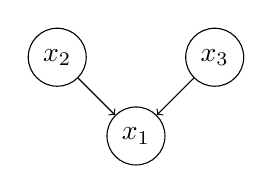
\begin{tikzpicture}
  % Define the nodes
  \node[circle, draw] (0) at (0, 0) {\(x_{1}\)};
  \node[circle, draw] (1) at (-1, 1) {\(x_2\)};
  \node[circle, draw] (2) at (1, 1) {\(x_3\)};

  % Draw the arrows
  \draw[->] (1) -- (0);
  \draw[->] (2) -- (0);
\end{tikzpicture}
\label{fig:three_node_graph}
\caption{The three-node graph}
\end{figure}

Algebraically, this problem is solved by
\begin{equation}
x_{1}' = x_{2}+x_{3} \label{three_node_analytical_view}
\end{equation}


We first compute what the learnable parameter should be with, and without normalisation, and then we try to train the model and verify that we get the expected weights. The motivation behind this is to construct the simplest possible GNN problem and to solve it both by hand and computationally to understand how the GCN model works and how it learns.

Our edge weights are fixed to 1, which means all edges have equal weighting, \(e_{j, i}=1\) in eq \ref{GCN_AGG}. Since we only do one graph convolution towards the root, we can disregard the updates for the two children nodes and only look at the update that affects the root, which means we can set \(i=1\) as well in eq \ref{GCN_AGG}.

This leaves us with a linear function with one parameter as can be seen in eq \ref{three_node_solution}.
\begin{align} \label{three_node_solution}
  \mathbf{x}_1' &= \Theta \sum_{j \in \mathcal{N}(v) \cup \{1\}} \mathbf{x}_j,\ \Theta \in \mathbb{R}\\
   &= \Theta (x_{1} + x_{2} + x_{3}) \quad \text{note that } x_{1} = 0\\
                &= \Theta (x_{2} + x_{3}) \implies \Theta = 1
\end{align}

Next, we do the same for the normalised example, \(\hat{d}_{i}\) is the number of neighbours of node \(i\) plus one. This means, we have \(\hat{d}_{2} = \hat{d}_{3} = 1\) and \(\hat{d}_{1}=3\).
\begin{align}
  \mathbf{x}_1' &= \Theta \sum_{j \in \mathcal{N}(v) \cup \{i\}} \frac{1}{\sqrt{\hat{d}_j \hat{d}_i}} \mathbf{x}_j\\
  &= \Theta  \left( \frac{1}{\sqrt{\hat{d}_2 \hat{d}_1}} \mathbf{x}_2 +  \frac{1}{\sqrt{\hat{d}_3 \hat{d}_1}} \mathbf{x}_3 \right)\\
  &= \Theta  \left( \frac{1}{\sqrt{1 \cdot 3}} \mathbf{x}_2 +  \frac{1}{\sqrt{1 \cdot 3}} \mathbf{x}_3 \right)\\
  &= \frac{\Theta}{\sqrt{3}}  \left(  \mathbf{x}_2 +   \mathbf{x}_3 \right) \implies \theta = \sqrt{3} \approx 1.732\\
\end{align}

SHOW RESULTS HERE (
Homework for Mustafa)

Next, we tried a classification problem, which also turned out to be slightly more complex. We reused the same graph. But this time we want to classify if \(x_{1} = x_{2}+x_{3}\) is true or not for the given graph. \(x_2, x_3\) are integers sampled from a uniform distribution in the range \([0, 10[\). Half of the generated graphs will have the property that \(x_{1} = x_{2}+x_{3}\) and the other half \(x_1\) is a random integer in the range \([0, 20[\). We mark the target class after generation to account for the case that that \(x_1\) is the sum of \(x_2\) and \(x_3\) also in the random case. [CALCULATE THE EXACT DISTRIBUTION OF THE CLASSES]

We tried with the same GCN model, here we got an accuracy of 48.5\%. Since this is close to the actual distribution of the classes, we can conclude that the model has not managed to learn the objective function.

The motivation of our following experiments is that we want the aggregator to find the difference between the children nodes and the root node. Hence we want to add the neighbours to the root but subtract the root node itself. Hence the self loop needs a separate weight parameter.

Hence we tried using a SAGE model, this is the same as the GCN model but with
an additional weight parameter for the self-loop, we also gave it a bias parameter. We got an accuracy of 53\%. % aber why do we give it a bias parameter?
This is not much better than the GCN model.

The models fail to learn since we have no non-linearity in the model. We need some behaviour
that allows the model to learn that the further away from 0 the difference is,
the more likely it is that the children nodes don't sum to the root node.
Therefore, we want a function that maps 0 to 1 and values further away from 0 to 0. 
For this, we simply chose the gaussian function \(e^{-x^2}\) which we
appended to the readout of the model. With this we get perfect results with an
accuracy of 100\%. On the downside, this model is very likely to not converge to an optimal solution: SHOW PLOT.

We then used the function \(1-x^{2}\) which we composed with the readout. This was also able to get perfect accuracy but it was much more stable and only in rare cases it would result in a suboptimal solution of >95\%.
accuracy of 100\%.

Even still we notice that our model is really unstable, most of the time, it never converges on a solution. Since it only has two parameters, we can actually plot the loss function in 3D and analytically investigate the issue. As can be seen on figure \ref{fig:loss_surface}, there are two local minima, in the quadrant where the model parameters are both negative and positive. 

\begin{figure}[H]
  \centering
  %% Creator: Matplotlib, PGF backend
%%
%% To include the figure in your LaTeX document, write
%%   \input{<filename>.pgf}
%%
%% Make sure the required packages are loaded in your preamble
%%   \usepackage{pgf}
%%
%% Also ensure that all the required font packages are loaded; for instance,
%% the lmodern package is sometimes necessary when using math font.
%%   \usepackage{lmodern}
%%
%% Figures using additional raster images can only be included by \input if
%% they are in the same directory as the main LaTeX file. For loading figures
%% from other directories you can use the `import` package
%%   \usepackage{import}
%%
%% and then include the figures with
%%   \import{<path to file>}{<filename>.pgf}
%%
%% Matplotlib used the following preamble
%%   \def\mathdefault#1{#1}
%%   \everymath=\expandafter{\the\everymath\displaystyle}
%%   
%%   \ifdefined\pdftexversion\else  % non-pdftex case.
%%     \usepackage{fontspec}
%%     \setmainfont{DejaVuSerif.ttf}[Path=\detokenize{/home/mustafah/.cache/pypoetry/virtualenvs/bachelor-project-92C-YcGL-py3.12/lib/python3.12/site-packages/matplotlib/mpl-data/fonts/ttf/}]
%%     \setsansfont{DejaVuSans.ttf}[Path=\detokenize{/home/mustafah/.cache/pypoetry/virtualenvs/bachelor-project-92C-YcGL-py3.12/lib/python3.12/site-packages/matplotlib/mpl-data/fonts/ttf/}]
%%     \setmonofont{DejaVuSansMono.ttf}[Path=\detokenize{/home/mustafah/.cache/pypoetry/virtualenvs/bachelor-project-92C-YcGL-py3.12/lib/python3.12/site-packages/matplotlib/mpl-data/fonts/ttf/}]
%%   \fi
%%   \makeatletter\@ifpackageloaded{underscore}{}{\usepackage[strings]{underscore}}\makeatother
%%
\begingroup%
\makeatletter%
\begin{pgfpicture}%
\pgfpathrectangle{\pgfpointorigin}{\pgfqpoint{6.400000in}{4.800000in}}%
\pgfusepath{use as bounding box, clip}%
\begin{pgfscope}%
\pgfsetbuttcap%
\pgfsetmiterjoin%
\definecolor{currentfill}{rgb}{1.000000,1.000000,1.000000}%
\pgfsetfillcolor{currentfill}%
\pgfsetlinewidth{0.000000pt}%
\definecolor{currentstroke}{rgb}{1.000000,1.000000,1.000000}%
\pgfsetstrokecolor{currentstroke}%
\pgfsetdash{}{0pt}%
\pgfpathmoveto{\pgfqpoint{0.000000in}{0.000000in}}%
\pgfpathlineto{\pgfqpoint{6.400000in}{0.000000in}}%
\pgfpathlineto{\pgfqpoint{6.400000in}{4.800000in}}%
\pgfpathlineto{\pgfqpoint{0.000000in}{4.800000in}}%
\pgfpathlineto{\pgfqpoint{0.000000in}{0.000000in}}%
\pgfpathclose%
\pgfusepath{fill}%
\end{pgfscope}%
\begin{pgfscope}%
\pgfsetbuttcap%
\pgfsetmiterjoin%
\definecolor{currentfill}{rgb}{1.000000,1.000000,1.000000}%
\pgfsetfillcolor{currentfill}%
\pgfsetlinewidth{0.000000pt}%
\definecolor{currentstroke}{rgb}{0.000000,0.000000,0.000000}%
\pgfsetstrokecolor{currentstroke}%
\pgfsetstrokeopacity{0.000000}%
\pgfsetdash{}{0pt}%
\pgfpathmoveto{\pgfqpoint{1.432000in}{0.528000in}}%
\pgfpathlineto{\pgfqpoint{5.128000in}{0.528000in}}%
\pgfpathlineto{\pgfqpoint{5.128000in}{4.224000in}}%
\pgfpathlineto{\pgfqpoint{1.432000in}{4.224000in}}%
\pgfpathlineto{\pgfqpoint{1.432000in}{0.528000in}}%
\pgfpathclose%
\pgfusepath{fill}%
\end{pgfscope}%
\begin{pgfscope}%
\pgfsetbuttcap%
\pgfsetmiterjoin%
\definecolor{currentfill}{rgb}{0.950000,0.950000,0.950000}%
\pgfsetfillcolor{currentfill}%
\pgfsetfillopacity{0.500000}%
\pgfsetlinewidth{1.003750pt}%
\definecolor{currentstroke}{rgb}{0.950000,0.950000,0.950000}%
\pgfsetstrokecolor{currentstroke}%
\pgfsetstrokeopacity{0.500000}%
\pgfsetdash{}{0pt}%
\pgfpathmoveto{\pgfqpoint{1.711073in}{1.439315in}}%
\pgfpathlineto{\pgfqpoint{2.931613in}{2.462396in}}%
\pgfpathlineto{\pgfqpoint{2.914647in}{3.937861in}}%
\pgfpathlineto{\pgfqpoint{1.635698in}{3.004542in}}%
\pgfusepath{stroke,fill}%
\end{pgfscope}%
\begin{pgfscope}%
\pgfsetbuttcap%
\pgfsetmiterjoin%
\definecolor{currentfill}{rgb}{0.900000,0.900000,0.900000}%
\pgfsetfillcolor{currentfill}%
\pgfsetfillopacity{0.500000}%
\pgfsetlinewidth{1.003750pt}%
\definecolor{currentstroke}{rgb}{0.900000,0.900000,0.900000}%
\pgfsetstrokecolor{currentstroke}%
\pgfsetstrokeopacity{0.500000}%
\pgfsetdash{}{0pt}%
\pgfpathmoveto{\pgfqpoint{2.931613in}{2.462396in}}%
\pgfpathlineto{\pgfqpoint{4.890144in}{1.893128in}}%
\pgfpathlineto{\pgfqpoint{4.960038in}{3.419414in}}%
\pgfpathlineto{\pgfqpoint{2.914647in}{3.937861in}}%
\pgfusepath{stroke,fill}%
\end{pgfscope}%
\begin{pgfscope}%
\pgfsetbuttcap%
\pgfsetmiterjoin%
\definecolor{currentfill}{rgb}{0.925000,0.925000,0.925000}%
\pgfsetfillcolor{currentfill}%
\pgfsetfillopacity{0.500000}%
\pgfsetlinewidth{1.003750pt}%
\definecolor{currentstroke}{rgb}{0.925000,0.925000,0.925000}%
\pgfsetstrokecolor{currentstroke}%
\pgfsetstrokeopacity{0.500000}%
\pgfsetdash{}{0pt}%
\pgfpathmoveto{\pgfqpoint{1.711073in}{1.439315in}}%
\pgfpathlineto{\pgfqpoint{3.787212in}{0.761248in}}%
\pgfpathlineto{\pgfqpoint{4.890144in}{1.893128in}}%
\pgfpathlineto{\pgfqpoint{2.931613in}{2.462396in}}%
\pgfusepath{stroke,fill}%
\end{pgfscope}%
\begin{pgfscope}%
\pgfsetbuttcap%
\pgfsetroundjoin%
\pgfsetlinewidth{0.803000pt}%
\definecolor{currentstroke}{rgb}{0.690196,0.690196,0.690196}%
\pgfsetstrokecolor{currentstroke}%
\pgfsetdash{}{0pt}%
\pgfpathmoveto{\pgfqpoint{1.836815in}{1.398248in}}%
\pgfpathlineto{\pgfqpoint{3.050725in}{2.427775in}}%
\pgfpathlineto{\pgfqpoint{3.038795in}{3.906393in}}%
\pgfusepath{stroke}%
\end{pgfscope}%
\begin{pgfscope}%
\pgfsetbuttcap%
\pgfsetroundjoin%
\pgfsetlinewidth{0.803000pt}%
\definecolor{currentstroke}{rgb}{0.690196,0.690196,0.690196}%
\pgfsetstrokecolor{currentstroke}%
\pgfsetdash{}{0pt}%
\pgfpathmoveto{\pgfqpoint{2.274263in}{1.255377in}}%
\pgfpathlineto{\pgfqpoint{3.464611in}{2.307474in}}%
\pgfpathlineto{\pgfqpoint{3.470428in}{3.796987in}}%
\pgfusepath{stroke}%
\end{pgfscope}%
\begin{pgfscope}%
\pgfsetbuttcap%
\pgfsetroundjoin%
\pgfsetlinewidth{0.803000pt}%
\definecolor{currentstroke}{rgb}{0.690196,0.690196,0.690196}%
\pgfsetstrokecolor{currentstroke}%
\pgfsetdash{}{0pt}%
\pgfpathmoveto{\pgfqpoint{2.721776in}{1.109220in}}%
\pgfpathlineto{\pgfqpoint{3.887223in}{2.184638in}}%
\pgfpathlineto{\pgfqpoint{3.911558in}{3.685173in}}%
\pgfusepath{stroke}%
\end{pgfscope}%
\begin{pgfscope}%
\pgfsetbuttcap%
\pgfsetroundjoin%
\pgfsetlinewidth{0.803000pt}%
\definecolor{currentstroke}{rgb}{0.690196,0.690196,0.690196}%
\pgfsetstrokecolor{currentstroke}%
\pgfsetdash{}{0pt}%
\pgfpathmoveto{\pgfqpoint{3.179705in}{0.959660in}}%
\pgfpathlineto{\pgfqpoint{4.318839in}{2.059184in}}%
\pgfpathlineto{\pgfqpoint{4.362503in}{3.570872in}}%
\pgfusepath{stroke}%
\end{pgfscope}%
\begin{pgfscope}%
\pgfsetbuttcap%
\pgfsetroundjoin%
\pgfsetlinewidth{0.803000pt}%
\definecolor{currentstroke}{rgb}{0.690196,0.690196,0.690196}%
\pgfsetstrokecolor{currentstroke}%
\pgfsetdash{}{0pt}%
\pgfpathmoveto{\pgfqpoint{3.648418in}{0.806579in}}%
\pgfpathlineto{\pgfqpoint{4.759751in}{1.931029in}}%
\pgfpathlineto{\pgfqpoint{4.823592in}{3.453999in}}%
\pgfusepath{stroke}%
\end{pgfscope}%
\begin{pgfscope}%
\pgfsetbuttcap%
\pgfsetroundjoin%
\pgfsetlinewidth{0.803000pt}%
\definecolor{currentstroke}{rgb}{0.690196,0.690196,0.690196}%
\pgfsetstrokecolor{currentstroke}%
\pgfsetdash{}{0pt}%
\pgfpathmoveto{\pgfqpoint{1.724140in}{3.069084in}}%
\pgfpathlineto{\pgfqpoint{1.795179in}{1.509814in}}%
\pgfpathlineto{\pgfqpoint{3.863526in}{0.839566in}}%
\pgfusepath{stroke}%
\end{pgfscope}%
\begin{pgfscope}%
\pgfsetbuttcap%
\pgfsetroundjoin%
\pgfsetlinewidth{0.803000pt}%
\definecolor{currentstroke}{rgb}{0.690196,0.690196,0.690196}%
\pgfsetstrokecolor{currentstroke}%
\pgfsetdash{}{0pt}%
\pgfpathmoveto{\pgfqpoint{2.019617in}{3.284710in}}%
\pgfpathlineto{\pgfqpoint{2.076487in}{1.745612in}}%
\pgfpathlineto{\pgfqpoint{4.118438in}{1.101167in}}%
\pgfusepath{stroke}%
\end{pgfscope}%
\begin{pgfscope}%
\pgfsetbuttcap%
\pgfsetroundjoin%
\pgfsetlinewidth{0.803000pt}%
\definecolor{currentstroke}{rgb}{0.690196,0.690196,0.690196}%
\pgfsetstrokecolor{currentstroke}%
\pgfsetdash{}{0pt}%
\pgfpathmoveto{\pgfqpoint{2.303622in}{3.491963in}}%
\pgfpathlineto{\pgfqpoint{2.347337in}{1.972644in}}%
\pgfpathlineto{\pgfqpoint{4.363383in}{1.352541in}}%
\pgfusepath{stroke}%
\end{pgfscope}%
\begin{pgfscope}%
\pgfsetbuttcap%
\pgfsetroundjoin%
\pgfsetlinewidth{0.803000pt}%
\definecolor{currentstroke}{rgb}{0.690196,0.690196,0.690196}%
\pgfsetstrokecolor{currentstroke}%
\pgfsetdash{}{0pt}%
\pgfpathmoveto{\pgfqpoint{2.576810in}{3.691323in}}%
\pgfpathlineto{\pgfqpoint{2.608303in}{2.191391in}}%
\pgfpathlineto{\pgfqpoint{4.598935in}{1.594276in}}%
\pgfusepath{stroke}%
\end{pgfscope}%
\begin{pgfscope}%
\pgfsetbuttcap%
\pgfsetroundjoin%
\pgfsetlinewidth{0.803000pt}%
\definecolor{currentstroke}{rgb}{0.690196,0.690196,0.690196}%
\pgfsetstrokecolor{currentstroke}%
\pgfsetdash{}{0pt}%
\pgfpathmoveto{\pgfqpoint{2.839787in}{3.883232in}}%
\pgfpathlineto{\pgfqpoint{2.859916in}{2.402298in}}%
\pgfpathlineto{\pgfqpoint{4.825625in}{1.826915in}}%
\pgfusepath{stroke}%
\end{pgfscope}%
\begin{pgfscope}%
\pgfsetbuttcap%
\pgfsetroundjoin%
\pgfsetlinewidth{0.803000pt}%
\definecolor{currentstroke}{rgb}{0.690196,0.690196,0.690196}%
\pgfsetstrokecolor{currentstroke}%
\pgfsetdash{}{0pt}%
\pgfpathmoveto{\pgfqpoint{4.890695in}{1.905158in}}%
\pgfpathlineto{\pgfqpoint{2.931479in}{2.474050in}}%
\pgfpathlineto{\pgfqpoint{1.710480in}{1.451632in}}%
\pgfusepath{stroke}%
\end{pgfscope}%
\begin{pgfscope}%
\pgfsetbuttcap%
\pgfsetroundjoin%
\pgfsetlinewidth{0.803000pt}%
\definecolor{currentstroke}{rgb}{0.690196,0.690196,0.690196}%
\pgfsetstrokecolor{currentstroke}%
\pgfsetdash{}{0pt}%
\pgfpathmoveto{\pgfqpoint{4.901070in}{2.131721in}}%
\pgfpathlineto{\pgfqpoint{2.928956in}{2.693455in}}%
\pgfpathlineto{\pgfqpoint{1.699307in}{1.683647in}}%
\pgfusepath{stroke}%
\end{pgfscope}%
\begin{pgfscope}%
\pgfsetbuttcap%
\pgfsetroundjoin%
\pgfsetlinewidth{0.803000pt}%
\definecolor{currentstroke}{rgb}{0.690196,0.690196,0.690196}%
\pgfsetstrokecolor{currentstroke}%
\pgfsetdash{}{0pt}%
\pgfpathmoveto{\pgfqpoint{4.911584in}{2.361315in}}%
\pgfpathlineto{\pgfqpoint{2.926401in}{2.915656in}}%
\pgfpathlineto{\pgfqpoint{1.687979in}{1.918886in}}%
\pgfusepath{stroke}%
\end{pgfscope}%
\begin{pgfscope}%
\pgfsetbuttcap%
\pgfsetroundjoin%
\pgfsetlinewidth{0.803000pt}%
\definecolor{currentstroke}{rgb}{0.690196,0.690196,0.690196}%
\pgfsetstrokecolor{currentstroke}%
\pgfsetdash{}{0pt}%
\pgfpathmoveto{\pgfqpoint{4.922240in}{2.594003in}}%
\pgfpathlineto{\pgfqpoint{2.923813in}{3.140707in}}%
\pgfpathlineto{\pgfqpoint{1.676492in}{2.157416in}}%
\pgfusepath{stroke}%
\end{pgfscope}%
\begin{pgfscope}%
\pgfsetbuttcap%
\pgfsetroundjoin%
\pgfsetlinewidth{0.803000pt}%
\definecolor{currentstroke}{rgb}{0.690196,0.690196,0.690196}%
\pgfsetstrokecolor{currentstroke}%
\pgfsetdash{}{0pt}%
\pgfpathmoveto{\pgfqpoint{4.933040in}{2.829847in}}%
\pgfpathlineto{\pgfqpoint{2.921192in}{3.368663in}}%
\pgfpathlineto{\pgfqpoint{1.664844in}{2.399308in}}%
\pgfusepath{stroke}%
\end{pgfscope}%
\begin{pgfscope}%
\pgfsetbuttcap%
\pgfsetroundjoin%
\pgfsetlinewidth{0.803000pt}%
\definecolor{currentstroke}{rgb}{0.690196,0.690196,0.690196}%
\pgfsetstrokecolor{currentstroke}%
\pgfsetdash{}{0pt}%
\pgfpathmoveto{\pgfqpoint{4.943987in}{3.068913in}}%
\pgfpathlineto{\pgfqpoint{2.918537in}{3.599581in}}%
\pgfpathlineto{\pgfqpoint{1.653030in}{2.644631in}}%
\pgfusepath{stroke}%
\end{pgfscope}%
\begin{pgfscope}%
\pgfsetbuttcap%
\pgfsetroundjoin%
\pgfsetlinewidth{0.803000pt}%
\definecolor{currentstroke}{rgb}{0.690196,0.690196,0.690196}%
\pgfsetstrokecolor{currentstroke}%
\pgfsetdash{}{0pt}%
\pgfpathmoveto{\pgfqpoint{4.955085in}{3.311266in}}%
\pgfpathlineto{\pgfqpoint{2.915847in}{3.833519in}}%
\pgfpathlineto{\pgfqpoint{1.641047in}{2.893461in}}%
\pgfusepath{stroke}%
\end{pgfscope}%
\begin{pgfscope}%
\pgfsetrectcap%
\pgfsetroundjoin%
\pgfsetlinewidth{0.803000pt}%
\definecolor{currentstroke}{rgb}{0.000000,0.000000,0.000000}%
\pgfsetstrokecolor{currentstroke}%
\pgfsetdash{}{0pt}%
\pgfpathmoveto{\pgfqpoint{1.711073in}{1.439315in}}%
\pgfpathlineto{\pgfqpoint{3.787212in}{0.761248in}}%
\pgfusepath{stroke}%
\end{pgfscope}%
\begin{pgfscope}%
\pgfsetrectcap%
\pgfsetroundjoin%
\pgfsetlinewidth{0.803000pt}%
\definecolor{currentstroke}{rgb}{0.000000,0.000000,0.000000}%
\pgfsetstrokecolor{currentstroke}%
\pgfsetdash{}{0pt}%
\pgfpathmoveto{\pgfqpoint{1.847386in}{1.407213in}}%
\pgfpathlineto{\pgfqpoint{1.815629in}{1.380279in}}%
\pgfusepath{stroke}%
\end{pgfscope}%
\begin{pgfscope}%
\definecolor{textcolor}{rgb}{0.000000,0.000000,0.000000}%
\pgfsetstrokecolor{textcolor}%
\pgfsetfillcolor{textcolor}%
\pgftext[x=1.732245in,y=1.180044in,,top]{\color{textcolor}{\sffamily\fontsize{10.000000}{12.000000}\selectfont\catcode`\^=\active\def^{\ifmmode\sp\else\^{}\fi}\catcode`\%=\active\def%{\%}\ensuremath{-}1.0}}%
\end{pgfscope}%
\begin{pgfscope}%
\pgfsetrectcap%
\pgfsetroundjoin%
\pgfsetlinewidth{0.803000pt}%
\definecolor{currentstroke}{rgb}{0.000000,0.000000,0.000000}%
\pgfsetstrokecolor{currentstroke}%
\pgfsetdash{}{0pt}%
\pgfpathmoveto{\pgfqpoint{2.284638in}{1.264547in}}%
\pgfpathlineto{\pgfqpoint{2.253468in}{1.236997in}}%
\pgfusepath{stroke}%
\end{pgfscope}%
\begin{pgfscope}%
\definecolor{textcolor}{rgb}{0.000000,0.000000,0.000000}%
\pgfsetstrokecolor{textcolor}%
\pgfsetfillcolor{textcolor}%
\pgftext[x=2.170144in,y=1.034145in,,top]{\color{textcolor}{\sffamily\fontsize{10.000000}{12.000000}\selectfont\catcode`\^=\active\def^{\ifmmode\sp\else\^{}\fi}\catcode`\%=\active\def%{\%}\ensuremath{-}0.5}}%
\end{pgfscope}%
\begin{pgfscope}%
\pgfsetrectcap%
\pgfsetroundjoin%
\pgfsetlinewidth{0.803000pt}%
\definecolor{currentstroke}{rgb}{0.000000,0.000000,0.000000}%
\pgfsetstrokecolor{currentstroke}%
\pgfsetdash{}{0pt}%
\pgfpathmoveto{\pgfqpoint{2.731944in}{1.118602in}}%
\pgfpathlineto{\pgfqpoint{2.701396in}{1.090414in}}%
\pgfusepath{stroke}%
\end{pgfscope}%
\begin{pgfscope}%
\definecolor{textcolor}{rgb}{0.000000,0.000000,0.000000}%
\pgfsetstrokecolor{textcolor}%
\pgfsetfillcolor{textcolor}%
\pgftext[x=2.618157in,y=0.884877in,,top]{\color{textcolor}{\sffamily\fontsize{10.000000}{12.000000}\selectfont\catcode`\^=\active\def^{\ifmmode\sp\else\^{}\fi}\catcode`\%=\active\def%{\%}0.0}}%
\end{pgfscope}%
\begin{pgfscope}%
\pgfsetrectcap%
\pgfsetroundjoin%
\pgfsetlinewidth{0.803000pt}%
\definecolor{currentstroke}{rgb}{0.000000,0.000000,0.000000}%
\pgfsetstrokecolor{currentstroke}%
\pgfsetdash{}{0pt}%
\pgfpathmoveto{\pgfqpoint{3.189653in}{0.969262in}}%
\pgfpathlineto{\pgfqpoint{3.159765in}{0.940414in}}%
\pgfusepath{stroke}%
\end{pgfscope}%
\begin{pgfscope}%
\definecolor{textcolor}{rgb}{0.000000,0.000000,0.000000}%
\pgfsetstrokecolor{textcolor}%
\pgfsetfillcolor{textcolor}%
\pgftext[x=3.076637in,y=0.732121in,,top]{\color{textcolor}{\sffamily\fontsize{10.000000}{12.000000}\selectfont\catcode`\^=\active\def^{\ifmmode\sp\else\^{}\fi}\catcode`\%=\active\def%{\%}0.5}}%
\end{pgfscope}%
\begin{pgfscope}%
\pgfsetrectcap%
\pgfsetroundjoin%
\pgfsetlinewidth{0.803000pt}%
\definecolor{currentstroke}{rgb}{0.000000,0.000000,0.000000}%
\pgfsetstrokecolor{currentstroke}%
\pgfsetdash{}{0pt}%
\pgfpathmoveto{\pgfqpoint{3.658132in}{0.816408in}}%
\pgfpathlineto{\pgfqpoint{3.628945in}{0.786876in}}%
\pgfusepath{stroke}%
\end{pgfscope}%
\begin{pgfscope}%
\definecolor{textcolor}{rgb}{0.000000,0.000000,0.000000}%
\pgfsetstrokecolor{textcolor}%
\pgfsetfillcolor{textcolor}%
\pgftext[x=3.545956in,y=0.575754in,,top]{\color{textcolor}{\sffamily\fontsize{10.000000}{12.000000}\selectfont\catcode`\^=\active\def^{\ifmmode\sp\else\^{}\fi}\catcode`\%=\active\def%{\%}1.0}}%
\end{pgfscope}%
\begin{pgfscope}%
\definecolor{textcolor}{rgb}{0.000000,0.000000,0.000000}%
\pgfsetstrokecolor{textcolor}%
\pgfsetfillcolor{textcolor}%
\pgftext[x=2.495506in,y=0.619330in,,]{\color{textcolor}{\sffamily\fontsize{10.000000}{12.000000}\selectfont\catcode`\^=\active\def^{\ifmmode\sp\else\^{}\fi}\catcode`\%=\active\def%{\%}w1}}%
\end{pgfscope}%
\begin{pgfscope}%
\pgfsetrectcap%
\pgfsetroundjoin%
\pgfsetlinewidth{0.803000pt}%
\definecolor{currentstroke}{rgb}{0.000000,0.000000,0.000000}%
\pgfsetstrokecolor{currentstroke}%
\pgfsetdash{}{0pt}%
\pgfpathmoveto{\pgfqpoint{4.890144in}{1.893128in}}%
\pgfpathlineto{\pgfqpoint{3.787212in}{0.761248in}}%
\pgfusepath{stroke}%
\end{pgfscope}%
\begin{pgfscope}%
\pgfsetrectcap%
\pgfsetroundjoin%
\pgfsetlinewidth{0.803000pt}%
\definecolor{currentstroke}{rgb}{0.000000,0.000000,0.000000}%
\pgfsetstrokecolor{currentstroke}%
\pgfsetdash{}{0pt}%
\pgfpathmoveto{\pgfqpoint{3.846096in}{0.845214in}}%
\pgfpathlineto{\pgfqpoint{3.898432in}{0.828255in}}%
\pgfusepath{stroke}%
\end{pgfscope}%
\begin{pgfscope}%
\definecolor{textcolor}{rgb}{0.000000,0.000000,0.000000}%
\pgfsetstrokecolor{textcolor}%
\pgfsetfillcolor{textcolor}%
\pgftext[x=4.042424in,y=0.653131in,,top]{\color{textcolor}{\sffamily\fontsize{10.000000}{12.000000}\selectfont\catcode`\^=\active\def^{\ifmmode\sp\else\^{}\fi}\catcode`\%=\active\def%{\%}\ensuremath{-}1.0}}%
\end{pgfscope}%
\begin{pgfscope}%
\pgfsetrectcap%
\pgfsetroundjoin%
\pgfsetlinewidth{0.803000pt}%
\definecolor{currentstroke}{rgb}{0.000000,0.000000,0.000000}%
\pgfsetstrokecolor{currentstroke}%
\pgfsetdash{}{0pt}%
\pgfpathmoveto{\pgfqpoint{4.101247in}{1.106592in}}%
\pgfpathlineto{\pgfqpoint{4.152862in}{1.090303in}}%
\pgfusepath{stroke}%
\end{pgfscope}%
\begin{pgfscope}%
\definecolor{textcolor}{rgb}{0.000000,0.000000,0.000000}%
\pgfsetstrokecolor{textcolor}%
\pgfsetfillcolor{textcolor}%
\pgftext[x=4.293916in,y=0.918605in,,top]{\color{textcolor}{\sffamily\fontsize{10.000000}{12.000000}\selectfont\catcode`\^=\active\def^{\ifmmode\sp\else\^{}\fi}\catcode`\%=\active\def%{\%}\ensuremath{-}0.5}}%
\end{pgfscope}%
\begin{pgfscope}%
\pgfsetrectcap%
\pgfsetroundjoin%
\pgfsetlinewidth{0.803000pt}%
\definecolor{currentstroke}{rgb}{0.000000,0.000000,0.000000}%
\pgfsetstrokecolor{currentstroke}%
\pgfsetdash{}{0pt}%
\pgfpathmoveto{\pgfqpoint{4.346427in}{1.357756in}}%
\pgfpathlineto{\pgfqpoint{4.397336in}{1.342097in}}%
\pgfusepath{stroke}%
\end{pgfscope}%
\begin{pgfscope}%
\definecolor{textcolor}{rgb}{0.000000,0.000000,0.000000}%
\pgfsetstrokecolor{textcolor}%
\pgfsetfillcolor{textcolor}%
\pgftext[x=4.535570in,y=1.173695in,,top]{\color{textcolor}{\sffamily\fontsize{10.000000}{12.000000}\selectfont\catcode`\^=\active\def^{\ifmmode\sp\else\^{}\fi}\catcode`\%=\active\def%{\%}0.0}}%
\end{pgfscope}%
\begin{pgfscope}%
\pgfsetrectcap%
\pgfsetroundjoin%
\pgfsetlinewidth{0.803000pt}%
\definecolor{currentstroke}{rgb}{0.000000,0.000000,0.000000}%
\pgfsetstrokecolor{currentstroke}%
\pgfsetdash{}{0pt}%
\pgfpathmoveto{\pgfqpoint{4.582209in}{1.599293in}}%
\pgfpathlineto{\pgfqpoint{4.632428in}{1.584229in}}%
\pgfusepath{stroke}%
\end{pgfscope}%
\begin{pgfscope}%
\definecolor{textcolor}{rgb}{0.000000,0.000000,0.000000}%
\pgfsetstrokecolor{textcolor}%
\pgfsetfillcolor{textcolor}%
\pgftext[x=4.767952in,y=1.418997in,,top]{\color{textcolor}{\sffamily\fontsize{10.000000}{12.000000}\selectfont\catcode`\^=\active\def^{\ifmmode\sp\else\^{}\fi}\catcode`\%=\active\def%{\%}0.5}}%
\end{pgfscope}%
\begin{pgfscope}%
\pgfsetrectcap%
\pgfsetroundjoin%
\pgfsetlinewidth{0.803000pt}%
\definecolor{currentstroke}{rgb}{0.000000,0.000000,0.000000}%
\pgfsetstrokecolor{currentstroke}%
\pgfsetdash{}{0pt}%
\pgfpathmoveto{\pgfqpoint{4.809123in}{1.831745in}}%
\pgfpathlineto{\pgfqpoint{4.858668in}{1.817243in}}%
\pgfusepath{stroke}%
\end{pgfscope}%
\begin{pgfscope}%
\definecolor{textcolor}{rgb}{0.000000,0.000000,0.000000}%
\pgfsetstrokecolor{textcolor}%
\pgfsetfillcolor{textcolor}%
\pgftext[x=4.991585in,y=1.655064in,,top]{\color{textcolor}{\sffamily\fontsize{10.000000}{12.000000}\selectfont\catcode`\^=\active\def^{\ifmmode\sp\else\^{}\fi}\catcode`\%=\active\def%{\%}1.0}}%
\end{pgfscope}%
\begin{pgfscope}%
\definecolor{textcolor}{rgb}{0.000000,0.000000,0.000000}%
\pgfsetstrokecolor{textcolor}%
\pgfsetfillcolor{textcolor}%
\pgftext[x=4.737955in,y=0.963482in,,]{\color{textcolor}{\sffamily\fontsize{10.000000}{12.000000}\selectfont\catcode`\^=\active\def^{\ifmmode\sp\else\^{}\fi}\catcode`\%=\active\def%{\%}w2}}%
\end{pgfscope}%
\begin{pgfscope}%
\pgfsetrectcap%
\pgfsetroundjoin%
\pgfsetlinewidth{0.803000pt}%
\definecolor{currentstroke}{rgb}{0.000000,0.000000,0.000000}%
\pgfsetstrokecolor{currentstroke}%
\pgfsetdash{}{0pt}%
\pgfpathmoveto{\pgfqpoint{4.890144in}{1.893128in}}%
\pgfpathlineto{\pgfqpoint{4.960038in}{3.419414in}}%
\pgfusepath{stroke}%
\end{pgfscope}%
\begin{pgfscope}%
\pgfsetrectcap%
\pgfsetroundjoin%
\pgfsetlinewidth{0.803000pt}%
\definecolor{currentstroke}{rgb}{0.000000,0.000000,0.000000}%
\pgfsetstrokecolor{currentstroke}%
\pgfsetdash{}{0pt}%
\pgfpathmoveto{\pgfqpoint{4.874252in}{1.909933in}}%
\pgfpathlineto{\pgfqpoint{4.923621in}{1.895598in}}%
\pgfusepath{stroke}%
\end{pgfscope}%
\begin{pgfscope}%
\definecolor{textcolor}{rgb}{0.000000,0.000000,0.000000}%
\pgfsetstrokecolor{textcolor}%
\pgfsetfillcolor{textcolor}%
\pgftext[x=5.144236in,y=1.941316in,,top]{\color{textcolor}{\sffamily\fontsize{10.000000}{12.000000}\selectfont\catcode`\^=\active\def^{\ifmmode\sp\else\^{}\fi}\catcode`\%=\active\def%{\%}0}}%
\end{pgfscope}%
\begin{pgfscope}%
\pgfsetrectcap%
\pgfsetroundjoin%
\pgfsetlinewidth{0.803000pt}%
\definecolor{currentstroke}{rgb}{0.000000,0.000000,0.000000}%
\pgfsetstrokecolor{currentstroke}%
\pgfsetdash{}{0pt}%
\pgfpathmoveto{\pgfqpoint{4.884513in}{2.136437in}}%
\pgfpathlineto{\pgfqpoint{4.934224in}{2.122277in}}%
\pgfusepath{stroke}%
\end{pgfscope}%
\begin{pgfscope}%
\definecolor{textcolor}{rgb}{0.000000,0.000000,0.000000}%
\pgfsetstrokecolor{textcolor}%
\pgfsetfillcolor{textcolor}%
\pgftext[x=5.156260in,y=2.167433in,,top]{\color{textcolor}{\sffamily\fontsize{10.000000}{12.000000}\selectfont\catcode`\^=\active\def^{\ifmmode\sp\else\^{}\fi}\catcode`\%=\active\def%{\%}10000}}%
\end{pgfscope}%
\begin{pgfscope}%
\pgfsetrectcap%
\pgfsetroundjoin%
\pgfsetlinewidth{0.803000pt}%
\definecolor{currentstroke}{rgb}{0.000000,0.000000,0.000000}%
\pgfsetstrokecolor{currentstroke}%
\pgfsetdash{}{0pt}%
\pgfpathmoveto{\pgfqpoint{4.894912in}{2.365970in}}%
\pgfpathlineto{\pgfqpoint{4.944968in}{2.351993in}}%
\pgfusepath{stroke}%
\end{pgfscope}%
\begin{pgfscope}%
\definecolor{textcolor}{rgb}{0.000000,0.000000,0.000000}%
\pgfsetstrokecolor{textcolor}%
\pgfsetfillcolor{textcolor}%
\pgftext[x=5.168445in,y=2.396568in,,top]{\color{textcolor}{\sffamily\fontsize{10.000000}{12.000000}\selectfont\catcode`\^=\active\def^{\ifmmode\sp\else\^{}\fi}\catcode`\%=\active\def%{\%}20000}}%
\end{pgfscope}%
\begin{pgfscope}%
\pgfsetrectcap%
\pgfsetroundjoin%
\pgfsetlinewidth{0.803000pt}%
\definecolor{currentstroke}{rgb}{0.000000,0.000000,0.000000}%
\pgfsetstrokecolor{currentstroke}%
\pgfsetdash{}{0pt}%
\pgfpathmoveto{\pgfqpoint{4.905451in}{2.598596in}}%
\pgfpathlineto{\pgfqpoint{4.955857in}{2.584806in}}%
\pgfusepath{stroke}%
\end{pgfscope}%
\begin{pgfscope}%
\definecolor{textcolor}{rgb}{0.000000,0.000000,0.000000}%
\pgfsetstrokecolor{textcolor}%
\pgfsetfillcolor{textcolor}%
\pgftext[x=5.180793in,y=2.628781in,,top]{\color{textcolor}{\sffamily\fontsize{10.000000}{12.000000}\selectfont\catcode`\^=\active\def^{\ifmmode\sp\else\^{}\fi}\catcode`\%=\active\def%{\%}30000}}%
\end{pgfscope}%
\begin{pgfscope}%
\pgfsetrectcap%
\pgfsetroundjoin%
\pgfsetlinewidth{0.803000pt}%
\definecolor{currentstroke}{rgb}{0.000000,0.000000,0.000000}%
\pgfsetstrokecolor{currentstroke}%
\pgfsetdash{}{0pt}%
\pgfpathmoveto{\pgfqpoint{4.916133in}{2.834375in}}%
\pgfpathlineto{\pgfqpoint{4.966894in}{2.820780in}}%
\pgfusepath{stroke}%
\end{pgfscope}%
\begin{pgfscope}%
\definecolor{textcolor}{rgb}{0.000000,0.000000,0.000000}%
\pgfsetstrokecolor{textcolor}%
\pgfsetfillcolor{textcolor}%
\pgftext[x=5.193308in,y=2.864134in,,top]{\color{textcolor}{\sffamily\fontsize{10.000000}{12.000000}\selectfont\catcode`\^=\active\def^{\ifmmode\sp\else\^{}\fi}\catcode`\%=\active\def%{\%}40000}}%
\end{pgfscope}%
\begin{pgfscope}%
\pgfsetrectcap%
\pgfsetroundjoin%
\pgfsetlinewidth{0.803000pt}%
\definecolor{currentstroke}{rgb}{0.000000,0.000000,0.000000}%
\pgfsetstrokecolor{currentstroke}%
\pgfsetdash{}{0pt}%
\pgfpathmoveto{\pgfqpoint{4.926960in}{3.073374in}}%
\pgfpathlineto{\pgfqpoint{4.978082in}{3.059980in}}%
\pgfusepath{stroke}%
\end{pgfscope}%
\begin{pgfscope}%
\definecolor{textcolor}{rgb}{0.000000,0.000000,0.000000}%
\pgfsetstrokecolor{textcolor}%
\pgfsetfillcolor{textcolor}%
\pgftext[x=5.205993in,y=3.102691in,,top]{\color{textcolor}{\sffamily\fontsize{10.000000}{12.000000}\selectfont\catcode`\^=\active\def^{\ifmmode\sp\else\^{}\fi}\catcode`\%=\active\def%{\%}50000}}%
\end{pgfscope}%
\begin{pgfscope}%
\pgfsetrectcap%
\pgfsetroundjoin%
\pgfsetlinewidth{0.803000pt}%
\definecolor{currentstroke}{rgb}{0.000000,0.000000,0.000000}%
\pgfsetstrokecolor{currentstroke}%
\pgfsetdash{}{0pt}%
\pgfpathmoveto{\pgfqpoint{4.937937in}{3.315658in}}%
\pgfpathlineto{\pgfqpoint{4.989424in}{3.302472in}}%
\pgfusepath{stroke}%
\end{pgfscope}%
\begin{pgfscope}%
\definecolor{textcolor}{rgb}{0.000000,0.000000,0.000000}%
\pgfsetstrokecolor{textcolor}%
\pgfsetfillcolor{textcolor}%
\pgftext[x=5.218852in,y=3.344519in,,top]{\color{textcolor}{\sffamily\fontsize{10.000000}{12.000000}\selectfont\catcode`\^=\active\def^{\ifmmode\sp\else\^{}\fi}\catcode`\%=\active\def%{\%}60000}}%
\end{pgfscope}%
\begin{pgfscope}%
\definecolor{textcolor}{rgb}{0.000000,0.000000,0.000000}%
\pgfsetstrokecolor{textcolor}%
\pgfsetfillcolor{textcolor}%
\pgftext[x=5.485100in,y=2.714682in,,]{\color{textcolor}{\sffamily\fontsize{10.000000}{12.000000}\selectfont\catcode`\^=\active\def^{\ifmmode\sp\else\^{}\fi}\catcode`\%=\active\def%{\%}Loss}}%
\end{pgfscope}%
\begin{pgfscope}%
\pgfpathrectangle{\pgfqpoint{1.432000in}{0.528000in}}{\pgfqpoint{3.696000in}{3.696000in}}%
\pgfusepath{clip}%
\pgfsetbuttcap%
\pgfsetroundjoin%
\definecolor{currentfill}{rgb}{0.267004,0.004874,0.329415}%
\pgfsetfillcolor{currentfill}%
\pgfsetlinewidth{0.000000pt}%
\definecolor{currentstroke}{rgb}{0.000000,0.000000,0.000000}%
\pgfsetstrokecolor{currentstroke}%
\pgfsetdash{}{0pt}%
\pgfpathmoveto{\pgfqpoint{2.927159in}{2.353550in}}%
\pgfpathlineto{\pgfqpoint{3.014186in}{2.326334in}}%
\pgfpathlineto{\pgfqpoint{3.065928in}{2.371709in}}%
\pgfpathlineto{\pgfqpoint{2.979147in}{2.395796in}}%
\pgfpathlineto{\pgfqpoint{2.927159in}{2.353550in}}%
\pgfpathclose%
\pgfusepath{fill}%
\end{pgfscope}%
\begin{pgfscope}%
\pgfpathrectangle{\pgfqpoint{1.432000in}{0.528000in}}{\pgfqpoint{3.696000in}{3.696000in}}%
\pgfusepath{clip}%
\pgfsetbuttcap%
\pgfsetroundjoin%
\definecolor{currentfill}{rgb}{0.267004,0.004874,0.329415}%
\pgfsetfillcolor{currentfill}%
\pgfsetlinewidth{0.000000pt}%
\definecolor{currentstroke}{rgb}{0.000000,0.000000,0.000000}%
\pgfsetstrokecolor{currentstroke}%
\pgfsetdash{}{0pt}%
\pgfpathmoveto{\pgfqpoint{3.014186in}{2.326334in}}%
\pgfpathlineto{\pgfqpoint{3.101569in}{2.301964in}}%
\pgfpathlineto{\pgfqpoint{3.153059in}{2.355065in}}%
\pgfpathlineto{\pgfqpoint{3.065928in}{2.371709in}}%
\pgfpathlineto{\pgfqpoint{3.014186in}{2.326334in}}%
\pgfpathclose%
\pgfusepath{fill}%
\end{pgfscope}%
\begin{pgfscope}%
\pgfpathrectangle{\pgfqpoint{1.432000in}{0.528000in}}{\pgfqpoint{3.696000in}{3.696000in}}%
\pgfusepath{clip}%
\pgfsetbuttcap%
\pgfsetroundjoin%
\definecolor{currentfill}{rgb}{0.267004,0.004874,0.329415}%
\pgfsetfillcolor{currentfill}%
\pgfsetlinewidth{0.000000pt}%
\definecolor{currentstroke}{rgb}{0.000000,0.000000,0.000000}%
\pgfsetstrokecolor{currentstroke}%
\pgfsetdash{}{0pt}%
\pgfpathmoveto{\pgfqpoint{2.874675in}{2.318084in}}%
\pgfpathlineto{\pgfqpoint{2.962020in}{2.283614in}}%
\pgfpathlineto{\pgfqpoint{3.014186in}{2.326334in}}%
\pgfpathlineto{\pgfqpoint{2.927159in}{2.353550in}}%
\pgfpathlineto{\pgfqpoint{2.874675in}{2.318084in}}%
\pgfpathclose%
\pgfusepath{fill}%
\end{pgfscope}%
\begin{pgfscope}%
\pgfpathrectangle{\pgfqpoint{1.432000in}{0.528000in}}{\pgfqpoint{3.696000in}{3.696000in}}%
\pgfusepath{clip}%
\pgfsetbuttcap%
\pgfsetroundjoin%
\definecolor{currentfill}{rgb}{0.269944,0.014625,0.341379}%
\pgfsetfillcolor{currentfill}%
\pgfsetlinewidth{0.000000pt}%
\definecolor{currentstroke}{rgb}{0.000000,0.000000,0.000000}%
\pgfsetstrokecolor{currentstroke}%
\pgfsetdash{}{0pt}%
\pgfpathmoveto{\pgfqpoint{3.101569in}{2.301964in}}%
\pgfpathlineto{\pgfqpoint{3.189313in}{2.285233in}}%
\pgfpathlineto{\pgfqpoint{3.240593in}{2.347827in}}%
\pgfpathlineto{\pgfqpoint{3.153059in}{2.355065in}}%
\pgfpathlineto{\pgfqpoint{3.101569in}{2.301964in}}%
\pgfpathclose%
\pgfusepath{fill}%
\end{pgfscope}%
\begin{pgfscope}%
\pgfpathrectangle{\pgfqpoint{1.432000in}{0.528000in}}{\pgfqpoint{3.696000in}{3.696000in}}%
\pgfusepath{clip}%
\pgfsetbuttcap%
\pgfsetroundjoin%
\definecolor{currentfill}{rgb}{0.267004,0.004874,0.329415}%
\pgfsetfillcolor{currentfill}%
\pgfsetlinewidth{0.000000pt}%
\definecolor{currentstroke}{rgb}{0.000000,0.000000,0.000000}%
\pgfsetstrokecolor{currentstroke}%
\pgfsetdash{}{0pt}%
\pgfpathmoveto{\pgfqpoint{2.962020in}{2.283614in}}%
\pgfpathlineto{\pgfqpoint{3.049649in}{2.256039in}}%
\pgfpathlineto{\pgfqpoint{3.101569in}{2.301964in}}%
\pgfpathlineto{\pgfqpoint{3.014186in}{2.326334in}}%
\pgfpathlineto{\pgfqpoint{2.962020in}{2.283614in}}%
\pgfpathclose%
\pgfusepath{fill}%
\end{pgfscope}%
\begin{pgfscope}%
\pgfpathrectangle{\pgfqpoint{1.432000in}{0.528000in}}{\pgfqpoint{3.696000in}{3.696000in}}%
\pgfusepath{clip}%
\pgfsetbuttcap%
\pgfsetroundjoin%
\definecolor{currentfill}{rgb}{0.274952,0.037752,0.364543}%
\pgfsetfillcolor{currentfill}%
\pgfsetlinewidth{0.000000pt}%
\definecolor{currentstroke}{rgb}{0.000000,0.000000,0.000000}%
\pgfsetstrokecolor{currentstroke}%
\pgfsetdash{}{0pt}%
\pgfpathmoveto{\pgfqpoint{3.189313in}{2.285233in}}%
\pgfpathlineto{\pgfqpoint{3.277477in}{2.277831in}}%
\pgfpathlineto{\pgfqpoint{3.328607in}{2.348989in}}%
\pgfpathlineto{\pgfqpoint{3.240593in}{2.347827in}}%
\pgfpathlineto{\pgfqpoint{3.189313in}{2.285233in}}%
\pgfpathclose%
\pgfusepath{fill}%
\end{pgfscope}%
\begin{pgfscope}%
\pgfpathrectangle{\pgfqpoint{1.432000in}{0.528000in}}{\pgfqpoint{3.696000in}{3.696000in}}%
\pgfusepath{clip}%
\pgfsetbuttcap%
\pgfsetroundjoin%
\definecolor{currentfill}{rgb}{0.269944,0.014625,0.341379}%
\pgfsetfillcolor{currentfill}%
\pgfsetlinewidth{0.000000pt}%
\definecolor{currentstroke}{rgb}{0.000000,0.000000,0.000000}%
\pgfsetstrokecolor{currentstroke}%
\pgfsetdash{}{0pt}%
\pgfpathmoveto{\pgfqpoint{2.821628in}{2.291430in}}%
\pgfpathlineto{\pgfqpoint{2.909362in}{2.247619in}}%
\pgfpathlineto{\pgfqpoint{2.962020in}{2.283614in}}%
\pgfpathlineto{\pgfqpoint{2.874675in}{2.318084in}}%
\pgfpathlineto{\pgfqpoint{2.821628in}{2.291430in}}%
\pgfpathclose%
\pgfusepath{fill}%
\end{pgfscope}%
\begin{pgfscope}%
\pgfpathrectangle{\pgfqpoint{1.432000in}{0.528000in}}{\pgfqpoint{3.696000in}{3.696000in}}%
\pgfusepath{clip}%
\pgfsetbuttcap%
\pgfsetroundjoin%
\definecolor{currentfill}{rgb}{0.267004,0.004874,0.329415}%
\pgfsetfillcolor{currentfill}%
\pgfsetlinewidth{0.000000pt}%
\definecolor{currentstroke}{rgb}{0.000000,0.000000,0.000000}%
\pgfsetstrokecolor{currentstroke}%
\pgfsetdash{}{0pt}%
\pgfpathmoveto{\pgfqpoint{3.049649in}{2.256039in}}%
\pgfpathlineto{\pgfqpoint{3.137642in}{2.231396in}}%
\pgfpathlineto{\pgfqpoint{3.189313in}{2.285233in}}%
\pgfpathlineto{\pgfqpoint{3.101569in}{2.301964in}}%
\pgfpathlineto{\pgfqpoint{3.049649in}{2.256039in}}%
\pgfpathclose%
\pgfusepath{fill}%
\end{pgfscope}%
\begin{pgfscope}%
\pgfpathrectangle{\pgfqpoint{1.432000in}{0.528000in}}{\pgfqpoint{3.696000in}{3.696000in}}%
\pgfusepath{clip}%
\pgfsetbuttcap%
\pgfsetroundjoin%
\definecolor{currentfill}{rgb}{0.267004,0.004874,0.329415}%
\pgfsetfillcolor{currentfill}%
\pgfsetlinewidth{0.000000pt}%
\definecolor{currentstroke}{rgb}{0.000000,0.000000,0.000000}%
\pgfsetstrokecolor{currentstroke}%
\pgfsetdash{}{0pt}%
\pgfpathmoveto{\pgfqpoint{2.909362in}{2.247619in}}%
\pgfpathlineto{\pgfqpoint{2.997305in}{2.212824in}}%
\pgfpathlineto{\pgfqpoint{3.049649in}{2.256039in}}%
\pgfpathlineto{\pgfqpoint{2.962020in}{2.283614in}}%
\pgfpathlineto{\pgfqpoint{2.909362in}{2.247619in}}%
\pgfpathclose%
\pgfusepath{fill}%
\end{pgfscope}%
\begin{pgfscope}%
\pgfpathrectangle{\pgfqpoint{1.432000in}{0.528000in}}{\pgfqpoint{3.696000in}{3.696000in}}%
\pgfusepath{clip}%
\pgfsetbuttcap%
\pgfsetroundjoin%
\definecolor{currentfill}{rgb}{0.279566,0.067836,0.391917}%
\pgfsetfillcolor{currentfill}%
\pgfsetlinewidth{0.000000pt}%
\definecolor{currentstroke}{rgb}{0.000000,0.000000,0.000000}%
\pgfsetstrokecolor{currentstroke}%
\pgfsetdash{}{0pt}%
\pgfpathmoveto{\pgfqpoint{3.277477in}{2.277831in}}%
\pgfpathlineto{\pgfqpoint{3.366137in}{2.278737in}}%
\pgfpathlineto{\pgfqpoint{3.417167in}{2.358055in}}%
\pgfpathlineto{\pgfqpoint{3.328607in}{2.348989in}}%
\pgfpathlineto{\pgfqpoint{3.277477in}{2.277831in}}%
\pgfpathclose%
\pgfusepath{fill}%
\end{pgfscope}%
\begin{pgfscope}%
\pgfpathrectangle{\pgfqpoint{1.432000in}{0.528000in}}{\pgfqpoint{3.696000in}{3.696000in}}%
\pgfusepath{clip}%
\pgfsetbuttcap%
\pgfsetroundjoin%
\definecolor{currentfill}{rgb}{0.269944,0.014625,0.341379}%
\pgfsetfillcolor{currentfill}%
\pgfsetlinewidth{0.000000pt}%
\definecolor{currentstroke}{rgb}{0.000000,0.000000,0.000000}%
\pgfsetstrokecolor{currentstroke}%
\pgfsetdash{}{0pt}%
\pgfpathmoveto{\pgfqpoint{3.137642in}{2.231396in}}%
\pgfpathlineto{\pgfqpoint{3.226008in}{2.214604in}}%
\pgfpathlineto{\pgfqpoint{3.277477in}{2.277831in}}%
\pgfpathlineto{\pgfqpoint{3.189313in}{2.285233in}}%
\pgfpathlineto{\pgfqpoint{3.137642in}{2.231396in}}%
\pgfpathclose%
\pgfusepath{fill}%
\end{pgfscope}%
\begin{pgfscope}%
\pgfpathrectangle{\pgfqpoint{1.432000in}{0.528000in}}{\pgfqpoint{3.696000in}{3.696000in}}%
\pgfusepath{clip}%
\pgfsetbuttcap%
\pgfsetroundjoin%
\definecolor{currentfill}{rgb}{0.267004,0.004874,0.329415}%
\pgfsetfillcolor{currentfill}%
\pgfsetlinewidth{0.000000pt}%
\definecolor{currentstroke}{rgb}{0.000000,0.000000,0.000000}%
\pgfsetstrokecolor{currentstroke}%
\pgfsetdash{}{0pt}%
\pgfpathmoveto{\pgfqpoint{2.997305in}{2.212824in}}%
\pgfpathlineto{\pgfqpoint{3.085544in}{2.184902in}}%
\pgfpathlineto{\pgfqpoint{3.137642in}{2.231396in}}%
\pgfpathlineto{\pgfqpoint{3.049649in}{2.256039in}}%
\pgfpathlineto{\pgfqpoint{2.997305in}{2.212824in}}%
\pgfpathclose%
\pgfusepath{fill}%
\end{pgfscope}%
\begin{pgfscope}%
\pgfpathrectangle{\pgfqpoint{1.432000in}{0.528000in}}{\pgfqpoint{3.696000in}{3.696000in}}%
\pgfusepath{clip}%
\pgfsetbuttcap%
\pgfsetroundjoin%
\definecolor{currentfill}{rgb}{0.274952,0.037752,0.364543}%
\pgfsetfillcolor{currentfill}%
\pgfsetlinewidth{0.000000pt}%
\definecolor{currentstroke}{rgb}{0.000000,0.000000,0.000000}%
\pgfsetstrokecolor{currentstroke}%
\pgfsetdash{}{0pt}%
\pgfpathmoveto{\pgfqpoint{2.767976in}{2.273210in}}%
\pgfpathlineto{\pgfqpoint{2.856140in}{2.220782in}}%
\pgfpathlineto{\pgfqpoint{2.909362in}{2.247619in}}%
\pgfpathlineto{\pgfqpoint{2.821628in}{2.291430in}}%
\pgfpathlineto{\pgfqpoint{2.767976in}{2.273210in}}%
\pgfpathclose%
\pgfusepath{fill}%
\end{pgfscope}%
\begin{pgfscope}%
\pgfpathrectangle{\pgfqpoint{1.432000in}{0.528000in}}{\pgfqpoint{3.696000in}{3.696000in}}%
\pgfusepath{clip}%
\pgfsetbuttcap%
\pgfsetroundjoin%
\definecolor{currentfill}{rgb}{0.274952,0.037752,0.364543}%
\pgfsetfillcolor{currentfill}%
\pgfsetlinewidth{0.000000pt}%
\definecolor{currentstroke}{rgb}{0.000000,0.000000,0.000000}%
\pgfsetstrokecolor{currentstroke}%
\pgfsetdash{}{0pt}%
\pgfpathmoveto{\pgfqpoint{3.226008in}{2.214604in}}%
\pgfpathlineto{\pgfqpoint{3.314812in}{2.207050in}}%
\pgfpathlineto{\pgfqpoint{3.366137in}{2.278737in}}%
\pgfpathlineto{\pgfqpoint{3.277477in}{2.277831in}}%
\pgfpathlineto{\pgfqpoint{3.226008in}{2.214604in}}%
\pgfpathclose%
\pgfusepath{fill}%
\end{pgfscope}%
\begin{pgfscope}%
\pgfpathrectangle{\pgfqpoint{1.432000in}{0.528000in}}{\pgfqpoint{3.696000in}{3.696000in}}%
\pgfusepath{clip}%
\pgfsetbuttcap%
\pgfsetroundjoin%
\definecolor{currentfill}{rgb}{0.282910,0.105393,0.426902}%
\pgfsetfillcolor{currentfill}%
\pgfsetlinewidth{0.000000pt}%
\definecolor{currentstroke}{rgb}{0.000000,0.000000,0.000000}%
\pgfsetstrokecolor{currentstroke}%
\pgfsetdash{}{0pt}%
\pgfpathmoveto{\pgfqpoint{3.366137in}{2.278737in}}%
\pgfpathlineto{\pgfqpoint{3.455360in}{2.287686in}}%
\pgfpathlineto{\pgfqpoint{3.506340in}{2.374842in}}%
\pgfpathlineto{\pgfqpoint{3.417167in}{2.358055in}}%
\pgfpathlineto{\pgfqpoint{3.366137in}{2.278737in}}%
\pgfpathclose%
\pgfusepath{fill}%
\end{pgfscope}%
\begin{pgfscope}%
\pgfpathrectangle{\pgfqpoint{1.432000in}{0.528000in}}{\pgfqpoint{3.696000in}{3.696000in}}%
\pgfusepath{clip}%
\pgfsetbuttcap%
\pgfsetroundjoin%
\definecolor{currentfill}{rgb}{0.269944,0.014625,0.341379}%
\pgfsetfillcolor{currentfill}%
\pgfsetlinewidth{0.000000pt}%
\definecolor{currentstroke}{rgb}{0.000000,0.000000,0.000000}%
\pgfsetstrokecolor{currentstroke}%
\pgfsetdash{}{0pt}%
\pgfpathmoveto{\pgfqpoint{2.856140in}{2.220782in}}%
\pgfpathlineto{\pgfqpoint{2.944470in}{2.176403in}}%
\pgfpathlineto{\pgfqpoint{2.997305in}{2.212824in}}%
\pgfpathlineto{\pgfqpoint{2.909362in}{2.247619in}}%
\pgfpathlineto{\pgfqpoint{2.856140in}{2.220782in}}%
\pgfpathclose%
\pgfusepath{fill}%
\end{pgfscope}%
\begin{pgfscope}%
\pgfpathrectangle{\pgfqpoint{1.432000in}{0.528000in}}{\pgfqpoint{3.696000in}{3.696000in}}%
\pgfusepath{clip}%
\pgfsetbuttcap%
\pgfsetroundjoin%
\definecolor{currentfill}{rgb}{0.267004,0.004874,0.329415}%
\pgfsetfillcolor{currentfill}%
\pgfsetlinewidth{0.000000pt}%
\definecolor{currentstroke}{rgb}{0.000000,0.000000,0.000000}%
\pgfsetstrokecolor{currentstroke}%
\pgfsetdash{}{0pt}%
\pgfpathmoveto{\pgfqpoint{3.085544in}{2.184902in}}%
\pgfpathlineto{\pgfqpoint{3.174154in}{2.160007in}}%
\pgfpathlineto{\pgfqpoint{3.226008in}{2.214604in}}%
\pgfpathlineto{\pgfqpoint{3.137642in}{2.231396in}}%
\pgfpathlineto{\pgfqpoint{3.085544in}{2.184902in}}%
\pgfpathclose%
\pgfusepath{fill}%
\end{pgfscope}%
\begin{pgfscope}%
\pgfpathrectangle{\pgfqpoint{1.432000in}{0.528000in}}{\pgfqpoint{3.696000in}{3.696000in}}%
\pgfusepath{clip}%
\pgfsetbuttcap%
\pgfsetroundjoin%
\definecolor{currentfill}{rgb}{0.267004,0.004874,0.329415}%
\pgfsetfillcolor{currentfill}%
\pgfsetlinewidth{0.000000pt}%
\definecolor{currentstroke}{rgb}{0.000000,0.000000,0.000000}%
\pgfsetstrokecolor{currentstroke}%
\pgfsetdash{}{0pt}%
\pgfpathmoveto{\pgfqpoint{2.944470in}{2.176403in}}%
\pgfpathlineto{\pgfqpoint{3.033020in}{2.141168in}}%
\pgfpathlineto{\pgfqpoint{3.085544in}{2.184902in}}%
\pgfpathlineto{\pgfqpoint{2.997305in}{2.212824in}}%
\pgfpathlineto{\pgfqpoint{2.944470in}{2.176403in}}%
\pgfpathclose%
\pgfusepath{fill}%
\end{pgfscope}%
\begin{pgfscope}%
\pgfpathrectangle{\pgfqpoint{1.432000in}{0.528000in}}{\pgfqpoint{3.696000in}{3.696000in}}%
\pgfusepath{clip}%
\pgfsetbuttcap%
\pgfsetroundjoin%
\definecolor{currentfill}{rgb}{0.279566,0.067836,0.391917}%
\pgfsetfillcolor{currentfill}%
\pgfsetlinewidth{0.000000pt}%
\definecolor{currentstroke}{rgb}{0.000000,0.000000,0.000000}%
\pgfsetstrokecolor{currentstroke}%
\pgfsetdash{}{0pt}%
\pgfpathmoveto{\pgfqpoint{3.314812in}{2.207050in}}%
\pgfpathlineto{\pgfqpoint{3.404127in}{2.207786in}}%
\pgfpathlineto{\pgfqpoint{3.455360in}{2.287686in}}%
\pgfpathlineto{\pgfqpoint{3.366137in}{2.278737in}}%
\pgfpathlineto{\pgfqpoint{3.314812in}{2.207050in}}%
\pgfpathclose%
\pgfusepath{fill}%
\end{pgfscope}%
\begin{pgfscope}%
\pgfpathrectangle{\pgfqpoint{1.432000in}{0.528000in}}{\pgfqpoint{3.696000in}{3.696000in}}%
\pgfusepath{clip}%
\pgfsetbuttcap%
\pgfsetroundjoin%
\definecolor{currentfill}{rgb}{0.269944,0.014625,0.341379}%
\pgfsetfillcolor{currentfill}%
\pgfsetlinewidth{0.000000pt}%
\definecolor{currentstroke}{rgb}{0.000000,0.000000,0.000000}%
\pgfsetstrokecolor{currentstroke}%
\pgfsetdash{}{0pt}%
\pgfpathmoveto{\pgfqpoint{3.174154in}{2.160007in}}%
\pgfpathlineto{\pgfqpoint{3.263152in}{2.143153in}}%
\pgfpathlineto{\pgfqpoint{3.314812in}{2.207050in}}%
\pgfpathlineto{\pgfqpoint{3.226008in}{2.214604in}}%
\pgfpathlineto{\pgfqpoint{3.174154in}{2.160007in}}%
\pgfpathclose%
\pgfusepath{fill}%
\end{pgfscope}%
\begin{pgfscope}%
\pgfpathrectangle{\pgfqpoint{1.432000in}{0.528000in}}{\pgfqpoint{3.696000in}{3.696000in}}%
\pgfusepath{clip}%
\pgfsetbuttcap%
\pgfsetroundjoin%
\definecolor{currentfill}{rgb}{0.279566,0.067836,0.391917}%
\pgfsetfillcolor{currentfill}%
\pgfsetlinewidth{0.000000pt}%
\definecolor{currentstroke}{rgb}{0.000000,0.000000,0.000000}%
\pgfsetstrokecolor{currentstroke}%
\pgfsetdash{}{0pt}%
\pgfpathmoveto{\pgfqpoint{2.713681in}{2.262867in}}%
\pgfpathlineto{\pgfqpoint{2.802320in}{2.202118in}}%
\pgfpathlineto{\pgfqpoint{2.856140in}{2.220782in}}%
\pgfpathlineto{\pgfqpoint{2.767976in}{2.273210in}}%
\pgfpathlineto{\pgfqpoint{2.713681in}{2.262867in}}%
\pgfpathclose%
\pgfusepath{fill}%
\end{pgfscope}%
\begin{pgfscope}%
\pgfpathrectangle{\pgfqpoint{1.432000in}{0.528000in}}{\pgfqpoint{3.696000in}{3.696000in}}%
\pgfusepath{clip}%
\pgfsetbuttcap%
\pgfsetroundjoin%
\definecolor{currentfill}{rgb}{0.281887,0.150881,0.465405}%
\pgfsetfillcolor{currentfill}%
\pgfsetlinewidth{0.000000pt}%
\definecolor{currentstroke}{rgb}{0.000000,0.000000,0.000000}%
\pgfsetstrokecolor{currentstroke}%
\pgfsetdash{}{0pt}%
\pgfpathmoveto{\pgfqpoint{3.455360in}{2.287686in}}%
\pgfpathlineto{\pgfqpoint{3.545209in}{2.303821in}}%
\pgfpathlineto{\pgfqpoint{3.596188in}{2.398984in}}%
\pgfpathlineto{\pgfqpoint{3.506340in}{2.374842in}}%
\pgfpathlineto{\pgfqpoint{3.455360in}{2.287686in}}%
\pgfpathclose%
\pgfusepath{fill}%
\end{pgfscope}%
\begin{pgfscope}%
\pgfpathrectangle{\pgfqpoint{1.432000in}{0.528000in}}{\pgfqpoint{3.696000in}{3.696000in}}%
\pgfusepath{clip}%
\pgfsetbuttcap%
\pgfsetroundjoin%
\definecolor{currentfill}{rgb}{0.267004,0.004874,0.329415}%
\pgfsetfillcolor{currentfill}%
\pgfsetlinewidth{0.000000pt}%
\definecolor{currentstroke}{rgb}{0.000000,0.000000,0.000000}%
\pgfsetstrokecolor{currentstroke}%
\pgfsetdash{}{0pt}%
\pgfpathmoveto{\pgfqpoint{3.033020in}{2.141168in}}%
\pgfpathlineto{\pgfqpoint{3.121878in}{2.112914in}}%
\pgfpathlineto{\pgfqpoint{3.174154in}{2.160007in}}%
\pgfpathlineto{\pgfqpoint{3.085544in}{2.184902in}}%
\pgfpathlineto{\pgfqpoint{3.033020in}{2.141168in}}%
\pgfpathclose%
\pgfusepath{fill}%
\end{pgfscope}%
\begin{pgfscope}%
\pgfpathrectangle{\pgfqpoint{1.432000in}{0.528000in}}{\pgfqpoint{3.696000in}{3.696000in}}%
\pgfusepath{clip}%
\pgfsetbuttcap%
\pgfsetroundjoin%
\definecolor{currentfill}{rgb}{0.274952,0.037752,0.364543}%
\pgfsetfillcolor{currentfill}%
\pgfsetlinewidth{0.000000pt}%
\definecolor{currentstroke}{rgb}{0.000000,0.000000,0.000000}%
\pgfsetstrokecolor{currentstroke}%
\pgfsetdash{}{0pt}%
\pgfpathmoveto{\pgfqpoint{2.802320in}{2.202118in}}%
\pgfpathlineto{\pgfqpoint{2.891076in}{2.149184in}}%
\pgfpathlineto{\pgfqpoint{2.944470in}{2.176403in}}%
\pgfpathlineto{\pgfqpoint{2.856140in}{2.220782in}}%
\pgfpathlineto{\pgfqpoint{2.802320in}{2.202118in}}%
\pgfpathclose%
\pgfusepath{fill}%
\end{pgfscope}%
\begin{pgfscope}%
\pgfpathrectangle{\pgfqpoint{1.432000in}{0.528000in}}{\pgfqpoint{3.696000in}{3.696000in}}%
\pgfusepath{clip}%
\pgfsetbuttcap%
\pgfsetroundjoin%
\definecolor{currentfill}{rgb}{0.274952,0.037752,0.364543}%
\pgfsetfillcolor{currentfill}%
\pgfsetlinewidth{0.000000pt}%
\definecolor{currentstroke}{rgb}{0.000000,0.000000,0.000000}%
\pgfsetstrokecolor{currentstroke}%
\pgfsetdash{}{0pt}%
\pgfpathmoveto{\pgfqpoint{3.263152in}{2.143153in}}%
\pgfpathlineto{\pgfqpoint{3.352605in}{2.135364in}}%
\pgfpathlineto{\pgfqpoint{3.404127in}{2.207786in}}%
\pgfpathlineto{\pgfqpoint{3.314812in}{2.207050in}}%
\pgfpathlineto{\pgfqpoint{3.263152in}{2.143153in}}%
\pgfpathclose%
\pgfusepath{fill}%
\end{pgfscope}%
\begin{pgfscope}%
\pgfpathrectangle{\pgfqpoint{1.432000in}{0.528000in}}{\pgfqpoint{3.696000in}{3.696000in}}%
\pgfusepath{clip}%
\pgfsetbuttcap%
\pgfsetroundjoin%
\definecolor{currentfill}{rgb}{0.282910,0.105393,0.426902}%
\pgfsetfillcolor{currentfill}%
\pgfsetlinewidth{0.000000pt}%
\definecolor{currentstroke}{rgb}{0.000000,0.000000,0.000000}%
\pgfsetstrokecolor{currentstroke}%
\pgfsetdash{}{0pt}%
\pgfpathmoveto{\pgfqpoint{3.404127in}{2.207786in}}%
\pgfpathlineto{\pgfqpoint{3.494020in}{2.216074in}}%
\pgfpathlineto{\pgfqpoint{3.545209in}{2.303821in}}%
\pgfpathlineto{\pgfqpoint{3.455360in}{2.287686in}}%
\pgfpathlineto{\pgfqpoint{3.404127in}{2.207786in}}%
\pgfpathclose%
\pgfusepath{fill}%
\end{pgfscope}%
\begin{pgfscope}%
\pgfpathrectangle{\pgfqpoint{1.432000in}{0.528000in}}{\pgfqpoint{3.696000in}{3.696000in}}%
\pgfusepath{clip}%
\pgfsetbuttcap%
\pgfsetroundjoin%
\definecolor{currentfill}{rgb}{0.269944,0.014625,0.341379}%
\pgfsetfillcolor{currentfill}%
\pgfsetlinewidth{0.000000pt}%
\definecolor{currentstroke}{rgb}{0.000000,0.000000,0.000000}%
\pgfsetstrokecolor{currentstroke}%
\pgfsetdash{}{0pt}%
\pgfpathmoveto{\pgfqpoint{2.891076in}{2.149184in}}%
\pgfpathlineto{\pgfqpoint{2.980007in}{2.104436in}}%
\pgfpathlineto{\pgfqpoint{3.033020in}{2.141168in}}%
\pgfpathlineto{\pgfqpoint{2.944470in}{2.176403in}}%
\pgfpathlineto{\pgfqpoint{2.891076in}{2.149184in}}%
\pgfpathclose%
\pgfusepath{fill}%
\end{pgfscope}%
\begin{pgfscope}%
\pgfpathrectangle{\pgfqpoint{1.432000in}{0.528000in}}{\pgfqpoint{3.696000in}{3.696000in}}%
\pgfusepath{clip}%
\pgfsetbuttcap%
\pgfsetroundjoin%
\definecolor{currentfill}{rgb}{0.267004,0.004874,0.329415}%
\pgfsetfillcolor{currentfill}%
\pgfsetlinewidth{0.000000pt}%
\definecolor{currentstroke}{rgb}{0.000000,0.000000,0.000000}%
\pgfsetstrokecolor{currentstroke}%
\pgfsetdash{}{0pt}%
\pgfpathmoveto{\pgfqpoint{3.121878in}{2.112914in}}%
\pgfpathlineto{\pgfqpoint{3.211115in}{2.087804in}}%
\pgfpathlineto{\pgfqpoint{3.263152in}{2.143153in}}%
\pgfpathlineto{\pgfqpoint{3.174154in}{2.160007in}}%
\pgfpathlineto{\pgfqpoint{3.121878in}{2.112914in}}%
\pgfpathclose%
\pgfusepath{fill}%
\end{pgfscope}%
\begin{pgfscope}%
\pgfpathrectangle{\pgfqpoint{1.432000in}{0.528000in}}{\pgfqpoint{3.696000in}{3.696000in}}%
\pgfusepath{clip}%
\pgfsetbuttcap%
\pgfsetroundjoin%
\definecolor{currentfill}{rgb}{0.274128,0.199721,0.498911}%
\pgfsetfillcolor{currentfill}%
\pgfsetlinewidth{0.000000pt}%
\definecolor{currentstroke}{rgb}{0.000000,0.000000,0.000000}%
\pgfsetstrokecolor{currentstroke}%
\pgfsetdash{}{0pt}%
\pgfpathmoveto{\pgfqpoint{3.545209in}{2.303821in}}%
\pgfpathlineto{\pgfqpoint{3.635754in}{2.328191in}}%
\pgfpathlineto{\pgfqpoint{3.686786in}{2.431744in}}%
\pgfpathlineto{\pgfqpoint{3.596188in}{2.398984in}}%
\pgfpathlineto{\pgfqpoint{3.545209in}{2.303821in}}%
\pgfpathclose%
\pgfusepath{fill}%
\end{pgfscope}%
\begin{pgfscope}%
\pgfpathrectangle{\pgfqpoint{1.432000in}{0.528000in}}{\pgfqpoint{3.696000in}{3.696000in}}%
\pgfusepath{clip}%
\pgfsetbuttcap%
\pgfsetroundjoin%
\definecolor{currentfill}{rgb}{0.282910,0.105393,0.426902}%
\pgfsetfillcolor{currentfill}%
\pgfsetlinewidth{0.000000pt}%
\definecolor{currentstroke}{rgb}{0.000000,0.000000,0.000000}%
\pgfsetstrokecolor{currentstroke}%
\pgfsetdash{}{0pt}%
\pgfpathmoveto{\pgfqpoint{2.658704in}{2.260019in}}%
\pgfpathlineto{\pgfqpoint{2.747864in}{2.191058in}}%
\pgfpathlineto{\pgfqpoint{2.802320in}{2.202118in}}%
\pgfpathlineto{\pgfqpoint{2.713681in}{2.262867in}}%
\pgfpathlineto{\pgfqpoint{2.658704in}{2.260019in}}%
\pgfpathclose%
\pgfusepath{fill}%
\end{pgfscope}%
\begin{pgfscope}%
\pgfpathrectangle{\pgfqpoint{1.432000in}{0.528000in}}{\pgfqpoint{3.696000in}{3.696000in}}%
\pgfusepath{clip}%
\pgfsetbuttcap%
\pgfsetroundjoin%
\definecolor{currentfill}{rgb}{0.267004,0.004874,0.329415}%
\pgfsetfillcolor{currentfill}%
\pgfsetlinewidth{0.000000pt}%
\definecolor{currentstroke}{rgb}{0.000000,0.000000,0.000000}%
\pgfsetstrokecolor{currentstroke}%
\pgfsetdash{}{0pt}%
\pgfpathmoveto{\pgfqpoint{2.980007in}{2.104436in}}%
\pgfpathlineto{\pgfqpoint{3.069175in}{2.068653in}}%
\pgfpathlineto{\pgfqpoint{3.121878in}{2.112914in}}%
\pgfpathlineto{\pgfqpoint{3.033020in}{2.141168in}}%
\pgfpathlineto{\pgfqpoint{2.980007in}{2.104436in}}%
\pgfpathclose%
\pgfusepath{fill}%
\end{pgfscope}%
\begin{pgfscope}%
\pgfpathrectangle{\pgfqpoint{1.432000in}{0.528000in}}{\pgfqpoint{3.696000in}{3.696000in}}%
\pgfusepath{clip}%
\pgfsetbuttcap%
\pgfsetroundjoin%
\definecolor{currentfill}{rgb}{0.279566,0.067836,0.391917}%
\pgfsetfillcolor{currentfill}%
\pgfsetlinewidth{0.000000pt}%
\definecolor{currentstroke}{rgb}{0.000000,0.000000,0.000000}%
\pgfsetstrokecolor{currentstroke}%
\pgfsetdash{}{0pt}%
\pgfpathmoveto{\pgfqpoint{3.352605in}{2.135364in}}%
\pgfpathlineto{\pgfqpoint{3.442585in}{2.135772in}}%
\pgfpathlineto{\pgfqpoint{3.494020in}{2.216074in}}%
\pgfpathlineto{\pgfqpoint{3.404127in}{2.207786in}}%
\pgfpathlineto{\pgfqpoint{3.352605in}{2.135364in}}%
\pgfpathclose%
\pgfusepath{fill}%
\end{pgfscope}%
\begin{pgfscope}%
\pgfpathrectangle{\pgfqpoint{1.432000in}{0.528000in}}{\pgfqpoint{3.696000in}{3.696000in}}%
\pgfusepath{clip}%
\pgfsetbuttcap%
\pgfsetroundjoin%
\definecolor{currentfill}{rgb}{0.269944,0.014625,0.341379}%
\pgfsetfillcolor{currentfill}%
\pgfsetlinewidth{0.000000pt}%
\definecolor{currentstroke}{rgb}{0.000000,0.000000,0.000000}%
\pgfsetstrokecolor{currentstroke}%
\pgfsetdash{}{0pt}%
\pgfpathmoveto{\pgfqpoint{3.211115in}{2.087804in}}%
\pgfpathlineto{\pgfqpoint{3.300754in}{2.070845in}}%
\pgfpathlineto{\pgfqpoint{3.352605in}{2.135364in}}%
\pgfpathlineto{\pgfqpoint{3.263152in}{2.143153in}}%
\pgfpathlineto{\pgfqpoint{3.211115in}{2.087804in}}%
\pgfpathclose%
\pgfusepath{fill}%
\end{pgfscope}%
\begin{pgfscope}%
\pgfpathrectangle{\pgfqpoint{1.432000in}{0.528000in}}{\pgfqpoint{3.696000in}{3.696000in}}%
\pgfusepath{clip}%
\pgfsetbuttcap%
\pgfsetroundjoin%
\definecolor{currentfill}{rgb}{0.279566,0.067836,0.391917}%
\pgfsetfillcolor{currentfill}%
\pgfsetlinewidth{0.000000pt}%
\definecolor{currentstroke}{rgb}{0.000000,0.000000,0.000000}%
\pgfsetstrokecolor{currentstroke}%
\pgfsetdash{}{0pt}%
\pgfpathmoveto{\pgfqpoint{2.747864in}{2.191058in}}%
\pgfpathlineto{\pgfqpoint{2.837088in}{2.130026in}}%
\pgfpathlineto{\pgfqpoint{2.891076in}{2.149184in}}%
\pgfpathlineto{\pgfqpoint{2.802320in}{2.202118in}}%
\pgfpathlineto{\pgfqpoint{2.747864in}{2.191058in}}%
\pgfpathclose%
\pgfusepath{fill}%
\end{pgfscope}%
\begin{pgfscope}%
\pgfpathrectangle{\pgfqpoint{1.432000in}{0.528000in}}{\pgfqpoint{3.696000in}{3.696000in}}%
\pgfusepath{clip}%
\pgfsetbuttcap%
\pgfsetroundjoin%
\definecolor{currentfill}{rgb}{0.281887,0.150881,0.465405}%
\pgfsetfillcolor{currentfill}%
\pgfsetlinewidth{0.000000pt}%
\definecolor{currentstroke}{rgb}{0.000000,0.000000,0.000000}%
\pgfsetstrokecolor{currentstroke}%
\pgfsetdash{}{0pt}%
\pgfpathmoveto{\pgfqpoint{3.494020in}{2.216074in}}%
\pgfpathlineto{\pgfqpoint{3.584557in}{2.232131in}}%
\pgfpathlineto{\pgfqpoint{3.635754in}{2.328191in}}%
\pgfpathlineto{\pgfqpoint{3.545209in}{2.303821in}}%
\pgfpathlineto{\pgfqpoint{3.494020in}{2.216074in}}%
\pgfpathclose%
\pgfusepath{fill}%
\end{pgfscope}%
\begin{pgfscope}%
\pgfpathrectangle{\pgfqpoint{1.432000in}{0.528000in}}{\pgfqpoint{3.696000in}{3.696000in}}%
\pgfusepath{clip}%
\pgfsetbuttcap%
\pgfsetroundjoin%
\definecolor{currentfill}{rgb}{0.267004,0.004874,0.329415}%
\pgfsetfillcolor{currentfill}%
\pgfsetlinewidth{0.000000pt}%
\definecolor{currentstroke}{rgb}{0.000000,0.000000,0.000000}%
\pgfsetstrokecolor{currentstroke}%
\pgfsetdash{}{0pt}%
\pgfpathmoveto{\pgfqpoint{3.069175in}{2.068653in}}%
\pgfpathlineto{\pgfqpoint{3.158660in}{2.040070in}}%
\pgfpathlineto{\pgfqpoint{3.211115in}{2.087804in}}%
\pgfpathlineto{\pgfqpoint{3.121878in}{2.112914in}}%
\pgfpathlineto{\pgfqpoint{3.069175in}{2.068653in}}%
\pgfpathclose%
\pgfusepath{fill}%
\end{pgfscope}%
\begin{pgfscope}%
\pgfpathrectangle{\pgfqpoint{1.432000in}{0.528000in}}{\pgfqpoint{3.696000in}{3.696000in}}%
\pgfusepath{clip}%
\pgfsetbuttcap%
\pgfsetroundjoin%
\definecolor{currentfill}{rgb}{0.274952,0.037752,0.364543}%
\pgfsetfillcolor{currentfill}%
\pgfsetlinewidth{0.000000pt}%
\definecolor{currentstroke}{rgb}{0.000000,0.000000,0.000000}%
\pgfsetstrokecolor{currentstroke}%
\pgfsetdash{}{0pt}%
\pgfpathmoveto{\pgfqpoint{2.837088in}{2.130026in}}%
\pgfpathlineto{\pgfqpoint{2.926442in}{2.076755in}}%
\pgfpathlineto{\pgfqpoint{2.980007in}{2.104436in}}%
\pgfpathlineto{\pgfqpoint{2.891076in}{2.149184in}}%
\pgfpathlineto{\pgfqpoint{2.837088in}{2.130026in}}%
\pgfpathclose%
\pgfusepath{fill}%
\end{pgfscope}%
\begin{pgfscope}%
\pgfpathrectangle{\pgfqpoint{1.432000in}{0.528000in}}{\pgfqpoint{3.696000in}{3.696000in}}%
\pgfusepath{clip}%
\pgfsetbuttcap%
\pgfsetroundjoin%
\definecolor{currentfill}{rgb}{0.257322,0.256130,0.526563}%
\pgfsetfillcolor{currentfill}%
\pgfsetlinewidth{0.000000pt}%
\definecolor{currentstroke}{rgb}{0.000000,0.000000,0.000000}%
\pgfsetstrokecolor{currentstroke}%
\pgfsetdash{}{0pt}%
\pgfpathmoveto{\pgfqpoint{3.635754in}{2.328191in}}%
\pgfpathlineto{\pgfqpoint{3.727067in}{2.360772in}}%
\pgfpathlineto{\pgfqpoint{3.778202in}{2.472620in}}%
\pgfpathlineto{\pgfqpoint{3.686786in}{2.431744in}}%
\pgfpathlineto{\pgfqpoint{3.635754in}{2.328191in}}%
\pgfpathclose%
\pgfusepath{fill}%
\end{pgfscope}%
\begin{pgfscope}%
\pgfpathrectangle{\pgfqpoint{1.432000in}{0.528000in}}{\pgfqpoint{3.696000in}{3.696000in}}%
\pgfusepath{clip}%
\pgfsetbuttcap%
\pgfsetroundjoin%
\definecolor{currentfill}{rgb}{0.274952,0.037752,0.364543}%
\pgfsetfillcolor{currentfill}%
\pgfsetlinewidth{0.000000pt}%
\definecolor{currentstroke}{rgb}{0.000000,0.000000,0.000000}%
\pgfsetstrokecolor{currentstroke}%
\pgfsetdash{}{0pt}%
\pgfpathmoveto{\pgfqpoint{3.300754in}{2.070845in}}%
\pgfpathlineto{\pgfqpoint{3.390865in}{2.062894in}}%
\pgfpathlineto{\pgfqpoint{3.442585in}{2.135772in}}%
\pgfpathlineto{\pgfqpoint{3.352605in}{2.135364in}}%
\pgfpathlineto{\pgfqpoint{3.300754in}{2.070845in}}%
\pgfpathclose%
\pgfusepath{fill}%
\end{pgfscope}%
\begin{pgfscope}%
\pgfpathrectangle{\pgfqpoint{1.432000in}{0.528000in}}{\pgfqpoint{3.696000in}{3.696000in}}%
\pgfusepath{clip}%
\pgfsetbuttcap%
\pgfsetroundjoin%
\definecolor{currentfill}{rgb}{0.282910,0.105393,0.426902}%
\pgfsetfillcolor{currentfill}%
\pgfsetlinewidth{0.000000pt}%
\definecolor{currentstroke}{rgb}{0.000000,0.000000,0.000000}%
\pgfsetstrokecolor{currentstroke}%
\pgfsetdash{}{0pt}%
\pgfpathmoveto{\pgfqpoint{3.442585in}{2.135772in}}%
\pgfpathlineto{\pgfqpoint{3.533157in}{2.143584in}}%
\pgfpathlineto{\pgfqpoint{3.584557in}{2.232131in}}%
\pgfpathlineto{\pgfqpoint{3.494020in}{2.216074in}}%
\pgfpathlineto{\pgfqpoint{3.442585in}{2.135772in}}%
\pgfpathclose%
\pgfusepath{fill}%
\end{pgfscope}%
\begin{pgfscope}%
\pgfpathrectangle{\pgfqpoint{1.432000in}{0.528000in}}{\pgfqpoint{3.696000in}{3.696000in}}%
\pgfusepath{clip}%
\pgfsetbuttcap%
\pgfsetroundjoin%
\definecolor{currentfill}{rgb}{0.269944,0.014625,0.341379}%
\pgfsetfillcolor{currentfill}%
\pgfsetlinewidth{0.000000pt}%
\definecolor{currentstroke}{rgb}{0.000000,0.000000,0.000000}%
\pgfsetstrokecolor{currentstroke}%
\pgfsetdash{}{0pt}%
\pgfpathmoveto{\pgfqpoint{2.926442in}{2.076755in}}%
\pgfpathlineto{\pgfqpoint{3.015984in}{2.031627in}}%
\pgfpathlineto{\pgfqpoint{3.069175in}{2.068653in}}%
\pgfpathlineto{\pgfqpoint{2.980007in}{2.104436in}}%
\pgfpathlineto{\pgfqpoint{2.926442in}{2.076755in}}%
\pgfpathclose%
\pgfusepath{fill}%
\end{pgfscope}%
\begin{pgfscope}%
\pgfpathrectangle{\pgfqpoint{1.432000in}{0.528000in}}{\pgfqpoint{3.696000in}{3.696000in}}%
\pgfusepath{clip}%
\pgfsetbuttcap%
\pgfsetroundjoin%
\definecolor{currentfill}{rgb}{0.267004,0.004874,0.329415}%
\pgfsetfillcolor{currentfill}%
\pgfsetlinewidth{0.000000pt}%
\definecolor{currentstroke}{rgb}{0.000000,0.000000,0.000000}%
\pgfsetstrokecolor{currentstroke}%
\pgfsetdash{}{0pt}%
\pgfpathmoveto{\pgfqpoint{3.158660in}{2.040070in}}%
\pgfpathlineto{\pgfqpoint{3.248532in}{2.014793in}}%
\pgfpathlineto{\pgfqpoint{3.300754in}{2.070845in}}%
\pgfpathlineto{\pgfqpoint{3.211115in}{2.087804in}}%
\pgfpathlineto{\pgfqpoint{3.158660in}{2.040070in}}%
\pgfpathclose%
\pgfusepath{fill}%
\end{pgfscope}%
\begin{pgfscope}%
\pgfpathrectangle{\pgfqpoint{1.432000in}{0.528000in}}{\pgfqpoint{3.696000in}{3.696000in}}%
\pgfusepath{clip}%
\pgfsetbuttcap%
\pgfsetroundjoin%
\definecolor{currentfill}{rgb}{0.281887,0.150881,0.465405}%
\pgfsetfillcolor{currentfill}%
\pgfsetlinewidth{0.000000pt}%
\definecolor{currentstroke}{rgb}{0.000000,0.000000,0.000000}%
\pgfsetstrokecolor{currentstroke}%
\pgfsetdash{}{0pt}%
\pgfpathmoveto{\pgfqpoint{2.603013in}{2.264179in}}%
\pgfpathlineto{\pgfqpoint{2.692735in}{2.187249in}}%
\pgfpathlineto{\pgfqpoint{2.747864in}{2.191058in}}%
\pgfpathlineto{\pgfqpoint{2.658704in}{2.260019in}}%
\pgfpathlineto{\pgfqpoint{2.603013in}{2.264179in}}%
\pgfpathclose%
\pgfusepath{fill}%
\end{pgfscope}%
\begin{pgfscope}%
\pgfpathrectangle{\pgfqpoint{1.432000in}{0.528000in}}{\pgfqpoint{3.696000in}{3.696000in}}%
\pgfusepath{clip}%
\pgfsetbuttcap%
\pgfsetroundjoin%
\definecolor{currentfill}{rgb}{0.274128,0.199721,0.498911}%
\pgfsetfillcolor{currentfill}%
\pgfsetlinewidth{0.000000pt}%
\definecolor{currentstroke}{rgb}{0.000000,0.000000,0.000000}%
\pgfsetstrokecolor{currentstroke}%
\pgfsetdash{}{0pt}%
\pgfpathmoveto{\pgfqpoint{3.584557in}{2.232131in}}%
\pgfpathlineto{\pgfqpoint{3.675808in}{2.256415in}}%
\pgfpathlineto{\pgfqpoint{3.727067in}{2.360772in}}%
\pgfpathlineto{\pgfqpoint{3.635754in}{2.328191in}}%
\pgfpathlineto{\pgfqpoint{3.584557in}{2.232131in}}%
\pgfpathclose%
\pgfusepath{fill}%
\end{pgfscope}%
\begin{pgfscope}%
\pgfpathrectangle{\pgfqpoint{1.432000in}{0.528000in}}{\pgfqpoint{3.696000in}{3.696000in}}%
\pgfusepath{clip}%
\pgfsetbuttcap%
\pgfsetroundjoin%
\definecolor{currentfill}{rgb}{0.282910,0.105393,0.426902}%
\pgfsetfillcolor{currentfill}%
\pgfsetlinewidth{0.000000pt}%
\definecolor{currentstroke}{rgb}{0.000000,0.000000,0.000000}%
\pgfsetstrokecolor{currentstroke}%
\pgfsetdash{}{0pt}%
\pgfpathmoveto{\pgfqpoint{2.692735in}{2.187249in}}%
\pgfpathlineto{\pgfqpoint{2.782474in}{2.118155in}}%
\pgfpathlineto{\pgfqpoint{2.837088in}{2.130026in}}%
\pgfpathlineto{\pgfqpoint{2.747864in}{2.191058in}}%
\pgfpathlineto{\pgfqpoint{2.692735in}{2.187249in}}%
\pgfpathclose%
\pgfusepath{fill}%
\end{pgfscope}%
\begin{pgfscope}%
\pgfpathrectangle{\pgfqpoint{1.432000in}{0.528000in}}{\pgfqpoint{3.696000in}{3.696000in}}%
\pgfusepath{clip}%
\pgfsetbuttcap%
\pgfsetroundjoin%
\definecolor{currentfill}{rgb}{0.267004,0.004874,0.329415}%
\pgfsetfillcolor{currentfill}%
\pgfsetlinewidth{0.000000pt}%
\definecolor{currentstroke}{rgb}{0.000000,0.000000,0.000000}%
\pgfsetstrokecolor{currentstroke}%
\pgfsetdash{}{0pt}%
\pgfpathmoveto{\pgfqpoint{3.015984in}{2.031627in}}%
\pgfpathlineto{\pgfqpoint{3.105776in}{1.995312in}}%
\pgfpathlineto{\pgfqpoint{3.158660in}{2.040070in}}%
\pgfpathlineto{\pgfqpoint{3.069175in}{2.068653in}}%
\pgfpathlineto{\pgfqpoint{3.015984in}{2.031627in}}%
\pgfpathclose%
\pgfusepath{fill}%
\end{pgfscope}%
\begin{pgfscope}%
\pgfpathrectangle{\pgfqpoint{1.432000in}{0.528000in}}{\pgfqpoint{3.696000in}{3.696000in}}%
\pgfusepath{clip}%
\pgfsetbuttcap%
\pgfsetroundjoin%
\definecolor{currentfill}{rgb}{0.279566,0.067836,0.391917}%
\pgfsetfillcolor{currentfill}%
\pgfsetlinewidth{0.000000pt}%
\definecolor{currentstroke}{rgb}{0.000000,0.000000,0.000000}%
\pgfsetstrokecolor{currentstroke}%
\pgfsetdash{}{0pt}%
\pgfpathmoveto{\pgfqpoint{3.390865in}{2.062894in}}%
\pgfpathlineto{\pgfqpoint{3.481517in}{2.062589in}}%
\pgfpathlineto{\pgfqpoint{3.533157in}{2.143584in}}%
\pgfpathlineto{\pgfqpoint{3.442585in}{2.135772in}}%
\pgfpathlineto{\pgfqpoint{3.390865in}{2.062894in}}%
\pgfpathclose%
\pgfusepath{fill}%
\end{pgfscope}%
\begin{pgfscope}%
\pgfpathrectangle{\pgfqpoint{1.432000in}{0.528000in}}{\pgfqpoint{3.696000in}{3.696000in}}%
\pgfusepath{clip}%
\pgfsetbuttcap%
\pgfsetroundjoin%
\definecolor{currentfill}{rgb}{0.231674,0.318106,0.544834}%
\pgfsetfillcolor{currentfill}%
\pgfsetlinewidth{0.000000pt}%
\definecolor{currentstroke}{rgb}{0.000000,0.000000,0.000000}%
\pgfsetstrokecolor{currentstroke}%
\pgfsetdash{}{0pt}%
\pgfpathmoveto{\pgfqpoint{3.727067in}{2.360772in}}%
\pgfpathlineto{\pgfqpoint{3.819200in}{2.400345in}}%
\pgfpathlineto{\pgfqpoint{3.870492in}{2.520648in}}%
\pgfpathlineto{\pgfqpoint{3.778202in}{2.472620in}}%
\pgfpathlineto{\pgfqpoint{3.727067in}{2.360772in}}%
\pgfpathclose%
\pgfusepath{fill}%
\end{pgfscope}%
\begin{pgfscope}%
\pgfpathrectangle{\pgfqpoint{1.432000in}{0.528000in}}{\pgfqpoint{3.696000in}{3.696000in}}%
\pgfusepath{clip}%
\pgfsetbuttcap%
\pgfsetroundjoin%
\definecolor{currentfill}{rgb}{0.269944,0.014625,0.341379}%
\pgfsetfillcolor{currentfill}%
\pgfsetlinewidth{0.000000pt}%
\definecolor{currentstroke}{rgb}{0.000000,0.000000,0.000000}%
\pgfsetstrokecolor{currentstroke}%
\pgfsetdash{}{0pt}%
\pgfpathmoveto{\pgfqpoint{3.248532in}{2.014793in}}%
\pgfpathlineto{\pgfqpoint{3.338822in}{1.997680in}}%
\pgfpathlineto{\pgfqpoint{3.390865in}{2.062894in}}%
\pgfpathlineto{\pgfqpoint{3.300754in}{2.070845in}}%
\pgfpathlineto{\pgfqpoint{3.248532in}{2.014793in}}%
\pgfpathclose%
\pgfusepath{fill}%
\end{pgfscope}%
\begin{pgfscope}%
\pgfpathrectangle{\pgfqpoint{1.432000in}{0.528000in}}{\pgfqpoint{3.696000in}{3.696000in}}%
\pgfusepath{clip}%
\pgfsetbuttcap%
\pgfsetroundjoin%
\definecolor{currentfill}{rgb}{0.279566,0.067836,0.391917}%
\pgfsetfillcolor{currentfill}%
\pgfsetlinewidth{0.000000pt}%
\definecolor{currentstroke}{rgb}{0.000000,0.000000,0.000000}%
\pgfsetstrokecolor{currentstroke}%
\pgfsetdash{}{0pt}%
\pgfpathmoveto{\pgfqpoint{2.782474in}{2.118155in}}%
\pgfpathlineto{\pgfqpoint{2.872290in}{2.056832in}}%
\pgfpathlineto{\pgfqpoint{2.926442in}{2.076755in}}%
\pgfpathlineto{\pgfqpoint{2.837088in}{2.130026in}}%
\pgfpathlineto{\pgfqpoint{2.782474in}{2.118155in}}%
\pgfpathclose%
\pgfusepath{fill}%
\end{pgfscope}%
\begin{pgfscope}%
\pgfpathrectangle{\pgfqpoint{1.432000in}{0.528000in}}{\pgfqpoint{3.696000in}{3.696000in}}%
\pgfusepath{clip}%
\pgfsetbuttcap%
\pgfsetroundjoin%
\definecolor{currentfill}{rgb}{0.281887,0.150881,0.465405}%
\pgfsetfillcolor{currentfill}%
\pgfsetlinewidth{0.000000pt}%
\definecolor{currentstroke}{rgb}{0.000000,0.000000,0.000000}%
\pgfsetstrokecolor{currentstroke}%
\pgfsetdash{}{0pt}%
\pgfpathmoveto{\pgfqpoint{3.533157in}{2.143584in}}%
\pgfpathlineto{\pgfqpoint{3.624391in}{2.159554in}}%
\pgfpathlineto{\pgfqpoint{3.675808in}{2.256415in}}%
\pgfpathlineto{\pgfqpoint{3.584557in}{2.232131in}}%
\pgfpathlineto{\pgfqpoint{3.533157in}{2.143584in}}%
\pgfpathclose%
\pgfusepath{fill}%
\end{pgfscope}%
\begin{pgfscope}%
\pgfpathrectangle{\pgfqpoint{1.432000in}{0.528000in}}{\pgfqpoint{3.696000in}{3.696000in}}%
\pgfusepath{clip}%
\pgfsetbuttcap%
\pgfsetroundjoin%
\definecolor{currentfill}{rgb}{0.267004,0.004874,0.329415}%
\pgfsetfillcolor{currentfill}%
\pgfsetlinewidth{0.000000pt}%
\definecolor{currentstroke}{rgb}{0.000000,0.000000,0.000000}%
\pgfsetstrokecolor{currentstroke}%
\pgfsetdash{}{0pt}%
\pgfpathmoveto{\pgfqpoint{3.105776in}{1.995312in}}%
\pgfpathlineto{\pgfqpoint{3.195897in}{1.966379in}}%
\pgfpathlineto{\pgfqpoint{3.248532in}{2.014793in}}%
\pgfpathlineto{\pgfqpoint{3.158660in}{2.040070in}}%
\pgfpathlineto{\pgfqpoint{3.105776in}{1.995312in}}%
\pgfpathclose%
\pgfusepath{fill}%
\end{pgfscope}%
\begin{pgfscope}%
\pgfpathrectangle{\pgfqpoint{1.432000in}{0.528000in}}{\pgfqpoint{3.696000in}{3.696000in}}%
\pgfusepath{clip}%
\pgfsetbuttcap%
\pgfsetroundjoin%
\definecolor{currentfill}{rgb}{0.274952,0.037752,0.364543}%
\pgfsetfillcolor{currentfill}%
\pgfsetlinewidth{0.000000pt}%
\definecolor{currentstroke}{rgb}{0.000000,0.000000,0.000000}%
\pgfsetstrokecolor{currentstroke}%
\pgfsetdash{}{0pt}%
\pgfpathmoveto{\pgfqpoint{2.872290in}{2.056832in}}%
\pgfpathlineto{\pgfqpoint{2.962247in}{2.003380in}}%
\pgfpathlineto{\pgfqpoint{3.015984in}{2.031627in}}%
\pgfpathlineto{\pgfqpoint{2.926442in}{2.076755in}}%
\pgfpathlineto{\pgfqpoint{2.872290in}{2.056832in}}%
\pgfpathclose%
\pgfusepath{fill}%
\end{pgfscope}%
\begin{pgfscope}%
\pgfpathrectangle{\pgfqpoint{1.432000in}{0.528000in}}{\pgfqpoint{3.696000in}{3.696000in}}%
\pgfusepath{clip}%
\pgfsetbuttcap%
\pgfsetroundjoin%
\definecolor{currentfill}{rgb}{0.257322,0.256130,0.526563}%
\pgfsetfillcolor{currentfill}%
\pgfsetlinewidth{0.000000pt}%
\definecolor{currentstroke}{rgb}{0.000000,0.000000,0.000000}%
\pgfsetstrokecolor{currentstroke}%
\pgfsetdash{}{0pt}%
\pgfpathmoveto{\pgfqpoint{3.675808in}{2.256415in}}%
\pgfpathlineto{\pgfqpoint{3.767829in}{2.287587in}}%
\pgfpathlineto{\pgfqpoint{3.819200in}{2.400345in}}%
\pgfpathlineto{\pgfqpoint{3.727067in}{2.360772in}}%
\pgfpathlineto{\pgfqpoint{3.675808in}{2.256415in}}%
\pgfpathclose%
\pgfusepath{fill}%
\end{pgfscope}%
\begin{pgfscope}%
\pgfpathrectangle{\pgfqpoint{1.432000in}{0.528000in}}{\pgfqpoint{3.696000in}{3.696000in}}%
\pgfusepath{clip}%
\pgfsetbuttcap%
\pgfsetroundjoin%
\definecolor{currentfill}{rgb}{0.274952,0.037752,0.364543}%
\pgfsetfillcolor{currentfill}%
\pgfsetlinewidth{0.000000pt}%
\definecolor{currentstroke}{rgb}{0.000000,0.000000,0.000000}%
\pgfsetstrokecolor{currentstroke}%
\pgfsetdash{}{0pt}%
\pgfpathmoveto{\pgfqpoint{3.338822in}{1.997680in}}%
\pgfpathlineto{\pgfqpoint{3.429600in}{1.989243in}}%
\pgfpathlineto{\pgfqpoint{3.481517in}{2.062589in}}%
\pgfpathlineto{\pgfqpoint{3.390865in}{2.062894in}}%
\pgfpathlineto{\pgfqpoint{3.338822in}{1.997680in}}%
\pgfpathclose%
\pgfusepath{fill}%
\end{pgfscope}%
\begin{pgfscope}%
\pgfpathrectangle{\pgfqpoint{1.432000in}{0.528000in}}{\pgfqpoint{3.696000in}{3.696000in}}%
\pgfusepath{clip}%
\pgfsetbuttcap%
\pgfsetroundjoin%
\definecolor{currentfill}{rgb}{0.282910,0.105393,0.426902}%
\pgfsetfillcolor{currentfill}%
\pgfsetlinewidth{0.000000pt}%
\definecolor{currentstroke}{rgb}{0.000000,0.000000,0.000000}%
\pgfsetstrokecolor{currentstroke}%
\pgfsetdash{}{0pt}%
\pgfpathmoveto{\pgfqpoint{3.481517in}{2.062589in}}%
\pgfpathlineto{\pgfqpoint{3.572779in}{2.070216in}}%
\pgfpathlineto{\pgfqpoint{3.624391in}{2.159554in}}%
\pgfpathlineto{\pgfqpoint{3.533157in}{2.143584in}}%
\pgfpathlineto{\pgfqpoint{3.481517in}{2.062589in}}%
\pgfpathclose%
\pgfusepath{fill}%
\end{pgfscope}%
\begin{pgfscope}%
\pgfpathrectangle{\pgfqpoint{1.432000in}{0.528000in}}{\pgfqpoint{3.696000in}{3.696000in}}%
\pgfusepath{clip}%
\pgfsetbuttcap%
\pgfsetroundjoin%
\definecolor{currentfill}{rgb}{0.274128,0.199721,0.498911}%
\pgfsetfillcolor{currentfill}%
\pgfsetlinewidth{0.000000pt}%
\definecolor{currentstroke}{rgb}{0.000000,0.000000,0.000000}%
\pgfsetstrokecolor{currentstroke}%
\pgfsetdash{}{0pt}%
\pgfpathmoveto{\pgfqpoint{2.546555in}{2.275680in}}%
\pgfpathlineto{\pgfqpoint{2.636897in}{2.190314in}}%
\pgfpathlineto{\pgfqpoint{2.692735in}{2.187249in}}%
\pgfpathlineto{\pgfqpoint{2.603013in}{2.264179in}}%
\pgfpathlineto{\pgfqpoint{2.546555in}{2.275680in}}%
\pgfpathclose%
\pgfusepath{fill}%
\end{pgfscope}%
\begin{pgfscope}%
\pgfpathrectangle{\pgfqpoint{1.432000in}{0.528000in}}{\pgfqpoint{3.696000in}{3.696000in}}%
\pgfusepath{clip}%
\pgfsetbuttcap%
\pgfsetroundjoin%
\definecolor{currentfill}{rgb}{0.269944,0.014625,0.341379}%
\pgfsetfillcolor{currentfill}%
\pgfsetlinewidth{0.000000pt}%
\definecolor{currentstroke}{rgb}{0.000000,0.000000,0.000000}%
\pgfsetstrokecolor{currentstroke}%
\pgfsetdash{}{0pt}%
\pgfpathmoveto{\pgfqpoint{2.962247in}{2.003380in}}%
\pgfpathlineto{\pgfqpoint{3.052407in}{1.957941in}}%
\pgfpathlineto{\pgfqpoint{3.105776in}{1.995312in}}%
\pgfpathlineto{\pgfqpoint{3.015984in}{2.031627in}}%
\pgfpathlineto{\pgfqpoint{2.962247in}{2.003380in}}%
\pgfpathclose%
\pgfusepath{fill}%
\end{pgfscope}%
\begin{pgfscope}%
\pgfpathrectangle{\pgfqpoint{1.432000in}{0.528000in}}{\pgfqpoint{3.696000in}{3.696000in}}%
\pgfusepath{clip}%
\pgfsetbuttcap%
\pgfsetroundjoin%
\definecolor{currentfill}{rgb}{0.267004,0.004874,0.329415}%
\pgfsetfillcolor{currentfill}%
\pgfsetlinewidth{0.000000pt}%
\definecolor{currentstroke}{rgb}{0.000000,0.000000,0.000000}%
\pgfsetstrokecolor{currentstroke}%
\pgfsetdash{}{0pt}%
\pgfpathmoveto{\pgfqpoint{3.195897in}{1.966379in}}%
\pgfpathlineto{\pgfqpoint{3.286414in}{1.940963in}}%
\pgfpathlineto{\pgfqpoint{3.338822in}{1.997680in}}%
\pgfpathlineto{\pgfqpoint{3.248532in}{2.014793in}}%
\pgfpathlineto{\pgfqpoint{3.195897in}{1.966379in}}%
\pgfpathclose%
\pgfusepath{fill}%
\end{pgfscope}%
\begin{pgfscope}%
\pgfpathrectangle{\pgfqpoint{1.432000in}{0.528000in}}{\pgfqpoint{3.696000in}{3.696000in}}%
\pgfusepath{clip}%
\pgfsetbuttcap%
\pgfsetroundjoin%
\definecolor{currentfill}{rgb}{0.281887,0.150881,0.465405}%
\pgfsetfillcolor{currentfill}%
\pgfsetlinewidth{0.000000pt}%
\definecolor{currentstroke}{rgb}{0.000000,0.000000,0.000000}%
\pgfsetstrokecolor{currentstroke}%
\pgfsetdash{}{0pt}%
\pgfpathmoveto{\pgfqpoint{2.636897in}{2.190314in}}%
\pgfpathlineto{\pgfqpoint{2.727200in}{2.112887in}}%
\pgfpathlineto{\pgfqpoint{2.782474in}{2.118155in}}%
\pgfpathlineto{\pgfqpoint{2.692735in}{2.187249in}}%
\pgfpathlineto{\pgfqpoint{2.636897in}{2.190314in}}%
\pgfpathclose%
\pgfusepath{fill}%
\end{pgfscope}%
\begin{pgfscope}%
\pgfpathrectangle{\pgfqpoint{1.432000in}{0.528000in}}{\pgfqpoint{3.696000in}{3.696000in}}%
\pgfusepath{clip}%
\pgfsetbuttcap%
\pgfsetroundjoin%
\definecolor{currentfill}{rgb}{0.274128,0.199721,0.498911}%
\pgfsetfillcolor{currentfill}%
\pgfsetlinewidth{0.000000pt}%
\definecolor{currentstroke}{rgb}{0.000000,0.000000,0.000000}%
\pgfsetstrokecolor{currentstroke}%
\pgfsetdash{}{0pt}%
\pgfpathmoveto{\pgfqpoint{3.624391in}{2.159554in}}%
\pgfpathlineto{\pgfqpoint{3.716344in}{2.182354in}}%
\pgfpathlineto{\pgfqpoint{3.767829in}{2.287587in}}%
\pgfpathlineto{\pgfqpoint{3.675808in}{2.256415in}}%
\pgfpathlineto{\pgfqpoint{3.624391in}{2.159554in}}%
\pgfpathclose%
\pgfusepath{fill}%
\end{pgfscope}%
\begin{pgfscope}%
\pgfpathrectangle{\pgfqpoint{1.432000in}{0.528000in}}{\pgfqpoint{3.696000in}{3.696000in}}%
\pgfusepath{clip}%
\pgfsetbuttcap%
\pgfsetroundjoin%
\definecolor{currentfill}{rgb}{0.204903,0.375746,0.553533}%
\pgfsetfillcolor{currentfill}%
\pgfsetlinewidth{0.000000pt}%
\definecolor{currentstroke}{rgb}{0.000000,0.000000,0.000000}%
\pgfsetstrokecolor{currentstroke}%
\pgfsetdash{}{0pt}%
\pgfpathmoveto{\pgfqpoint{3.819200in}{2.400345in}}%
\pgfpathlineto{\pgfqpoint{3.912223in}{2.447261in}}%
\pgfpathlineto{\pgfqpoint{3.963723in}{2.576014in}}%
\pgfpathlineto{\pgfqpoint{3.870492in}{2.520648in}}%
\pgfpathlineto{\pgfqpoint{3.819200in}{2.400345in}}%
\pgfpathclose%
\pgfusepath{fill}%
\end{pgfscope}%
\begin{pgfscope}%
\pgfpathrectangle{\pgfqpoint{1.432000in}{0.528000in}}{\pgfqpoint{3.696000in}{3.696000in}}%
\pgfusepath{clip}%
\pgfsetbuttcap%
\pgfsetroundjoin%
\definecolor{currentfill}{rgb}{0.282910,0.105393,0.426902}%
\pgfsetfillcolor{currentfill}%
\pgfsetlinewidth{0.000000pt}%
\definecolor{currentstroke}{rgb}{0.000000,0.000000,0.000000}%
\pgfsetstrokecolor{currentstroke}%
\pgfsetdash{}{0pt}%
\pgfpathmoveto{\pgfqpoint{2.727200in}{2.112887in}}%
\pgfpathlineto{\pgfqpoint{2.817527in}{2.043420in}}%
\pgfpathlineto{\pgfqpoint{2.872290in}{2.056832in}}%
\pgfpathlineto{\pgfqpoint{2.782474in}{2.118155in}}%
\pgfpathlineto{\pgfqpoint{2.727200in}{2.112887in}}%
\pgfpathclose%
\pgfusepath{fill}%
\end{pgfscope}%
\begin{pgfscope}%
\pgfpathrectangle{\pgfqpoint{1.432000in}{0.528000in}}{\pgfqpoint{3.696000in}{3.696000in}}%
\pgfusepath{clip}%
\pgfsetbuttcap%
\pgfsetroundjoin%
\definecolor{currentfill}{rgb}{0.267004,0.004874,0.329415}%
\pgfsetfillcolor{currentfill}%
\pgfsetlinewidth{0.000000pt}%
\definecolor{currentstroke}{rgb}{0.000000,0.000000,0.000000}%
\pgfsetstrokecolor{currentstroke}%
\pgfsetdash{}{0pt}%
\pgfpathmoveto{\pgfqpoint{3.052407in}{1.957941in}}%
\pgfpathlineto{\pgfqpoint{3.142833in}{1.921187in}}%
\pgfpathlineto{\pgfqpoint{3.195897in}{1.966379in}}%
\pgfpathlineto{\pgfqpoint{3.105776in}{1.995312in}}%
\pgfpathlineto{\pgfqpoint{3.052407in}{1.957941in}}%
\pgfpathclose%
\pgfusepath{fill}%
\end{pgfscope}%
\begin{pgfscope}%
\pgfpathrectangle{\pgfqpoint{1.432000in}{0.528000in}}{\pgfqpoint{3.696000in}{3.696000in}}%
\pgfusepath{clip}%
\pgfsetbuttcap%
\pgfsetroundjoin%
\definecolor{currentfill}{rgb}{0.279566,0.067836,0.391917}%
\pgfsetfillcolor{currentfill}%
\pgfsetlinewidth{0.000000pt}%
\definecolor{currentstroke}{rgb}{0.000000,0.000000,0.000000}%
\pgfsetstrokecolor{currentstroke}%
\pgfsetdash{}{0pt}%
\pgfpathmoveto{\pgfqpoint{3.429600in}{1.989243in}}%
\pgfpathlineto{\pgfqpoint{3.520934in}{1.988464in}}%
\pgfpathlineto{\pgfqpoint{3.572779in}{2.070216in}}%
\pgfpathlineto{\pgfqpoint{3.481517in}{2.062589in}}%
\pgfpathlineto{\pgfqpoint{3.429600in}{1.989243in}}%
\pgfpathclose%
\pgfusepath{fill}%
\end{pgfscope}%
\begin{pgfscope}%
\pgfpathrectangle{\pgfqpoint{1.432000in}{0.528000in}}{\pgfqpoint{3.696000in}{3.696000in}}%
\pgfusepath{clip}%
\pgfsetbuttcap%
\pgfsetroundjoin%
\definecolor{currentfill}{rgb}{0.233603,0.313828,0.543914}%
\pgfsetfillcolor{currentfill}%
\pgfsetlinewidth{0.000000pt}%
\definecolor{currentstroke}{rgb}{0.000000,0.000000,0.000000}%
\pgfsetstrokecolor{currentstroke}%
\pgfsetdash{}{0pt}%
\pgfpathmoveto{\pgfqpoint{3.767829in}{2.287587in}}%
\pgfpathlineto{\pgfqpoint{3.860689in}{2.326119in}}%
\pgfpathlineto{\pgfqpoint{3.912223in}{2.447261in}}%
\pgfpathlineto{\pgfqpoint{3.819200in}{2.400345in}}%
\pgfpathlineto{\pgfqpoint{3.767829in}{2.287587in}}%
\pgfpathclose%
\pgfusepath{fill}%
\end{pgfscope}%
\begin{pgfscope}%
\pgfpathrectangle{\pgfqpoint{1.432000in}{0.528000in}}{\pgfqpoint{3.696000in}{3.696000in}}%
\pgfusepath{clip}%
\pgfsetbuttcap%
\pgfsetroundjoin%
\definecolor{currentfill}{rgb}{0.269944,0.014625,0.341379}%
\pgfsetfillcolor{currentfill}%
\pgfsetlinewidth{0.000000pt}%
\definecolor{currentstroke}{rgb}{0.000000,0.000000,0.000000}%
\pgfsetstrokecolor{currentstroke}%
\pgfsetdash{}{0pt}%
\pgfpathmoveto{\pgfqpoint{3.286414in}{1.940963in}}%
\pgfpathlineto{\pgfqpoint{3.377365in}{1.923647in}}%
\pgfpathlineto{\pgfqpoint{3.429600in}{1.989243in}}%
\pgfpathlineto{\pgfqpoint{3.338822in}{1.997680in}}%
\pgfpathlineto{\pgfqpoint{3.286414in}{1.940963in}}%
\pgfpathclose%
\pgfusepath{fill}%
\end{pgfscope}%
\begin{pgfscope}%
\pgfpathrectangle{\pgfqpoint{1.432000in}{0.528000in}}{\pgfqpoint{3.696000in}{3.696000in}}%
\pgfusepath{clip}%
\pgfsetbuttcap%
\pgfsetroundjoin%
\definecolor{currentfill}{rgb}{0.279566,0.067836,0.391917}%
\pgfsetfillcolor{currentfill}%
\pgfsetlinewidth{0.000000pt}%
\definecolor{currentstroke}{rgb}{0.000000,0.000000,0.000000}%
\pgfsetstrokecolor{currentstroke}%
\pgfsetdash{}{0pt}%
\pgfpathmoveto{\pgfqpoint{2.817527in}{2.043420in}}%
\pgfpathlineto{\pgfqpoint{2.907941in}{1.981942in}}%
\pgfpathlineto{\pgfqpoint{2.962247in}{2.003380in}}%
\pgfpathlineto{\pgfqpoint{2.872290in}{2.056832in}}%
\pgfpathlineto{\pgfqpoint{2.817527in}{2.043420in}}%
\pgfpathclose%
\pgfusepath{fill}%
\end{pgfscope}%
\begin{pgfscope}%
\pgfpathrectangle{\pgfqpoint{1.432000in}{0.528000in}}{\pgfqpoint{3.696000in}{3.696000in}}%
\pgfusepath{clip}%
\pgfsetbuttcap%
\pgfsetroundjoin%
\definecolor{currentfill}{rgb}{0.281887,0.150881,0.465405}%
\pgfsetfillcolor{currentfill}%
\pgfsetlinewidth{0.000000pt}%
\definecolor{currentstroke}{rgb}{0.000000,0.000000,0.000000}%
\pgfsetstrokecolor{currentstroke}%
\pgfsetdash{}{0pt}%
\pgfpathmoveto{\pgfqpoint{3.572779in}{2.070216in}}%
\pgfpathlineto{\pgfqpoint{3.664708in}{2.084649in}}%
\pgfpathlineto{\pgfqpoint{3.716344in}{2.182354in}}%
\pgfpathlineto{\pgfqpoint{3.624391in}{2.159554in}}%
\pgfpathlineto{\pgfqpoint{3.572779in}{2.070216in}}%
\pgfpathclose%
\pgfusepath{fill}%
\end{pgfscope}%
\begin{pgfscope}%
\pgfpathrectangle{\pgfqpoint{1.432000in}{0.528000in}}{\pgfqpoint{3.696000in}{3.696000in}}%
\pgfusepath{clip}%
\pgfsetbuttcap%
\pgfsetroundjoin%
\definecolor{currentfill}{rgb}{0.267004,0.004874,0.329415}%
\pgfsetfillcolor{currentfill}%
\pgfsetlinewidth{0.000000pt}%
\definecolor{currentstroke}{rgb}{0.000000,0.000000,0.000000}%
\pgfsetstrokecolor{currentstroke}%
\pgfsetdash{}{0pt}%
\pgfpathmoveto{\pgfqpoint{3.142833in}{1.921187in}}%
\pgfpathlineto{\pgfqpoint{3.233599in}{1.891873in}}%
\pgfpathlineto{\pgfqpoint{3.286414in}{1.940963in}}%
\pgfpathlineto{\pgfqpoint{3.195897in}{1.966379in}}%
\pgfpathlineto{\pgfqpoint{3.142833in}{1.921187in}}%
\pgfpathclose%
\pgfusepath{fill}%
\end{pgfscope}%
\begin{pgfscope}%
\pgfpathrectangle{\pgfqpoint{1.432000in}{0.528000in}}{\pgfqpoint{3.696000in}{3.696000in}}%
\pgfusepath{clip}%
\pgfsetbuttcap%
\pgfsetroundjoin%
\definecolor{currentfill}{rgb}{0.274952,0.037752,0.364543}%
\pgfsetfillcolor{currentfill}%
\pgfsetlinewidth{0.000000pt}%
\definecolor{currentstroke}{rgb}{0.000000,0.000000,0.000000}%
\pgfsetstrokecolor{currentstroke}%
\pgfsetdash{}{0pt}%
\pgfpathmoveto{\pgfqpoint{2.907941in}{1.981942in}}%
\pgfpathlineto{\pgfqpoint{2.998506in}{1.928491in}}%
\pgfpathlineto{\pgfqpoint{3.052407in}{1.957941in}}%
\pgfpathlineto{\pgfqpoint{2.962247in}{2.003380in}}%
\pgfpathlineto{\pgfqpoint{2.907941in}{1.981942in}}%
\pgfpathclose%
\pgfusepath{fill}%
\end{pgfscope}%
\begin{pgfscope}%
\pgfpathrectangle{\pgfqpoint{1.432000in}{0.528000in}}{\pgfqpoint{3.696000in}{3.696000in}}%
\pgfusepath{clip}%
\pgfsetbuttcap%
\pgfsetroundjoin%
\definecolor{currentfill}{rgb}{0.257322,0.256130,0.526563}%
\pgfsetfillcolor{currentfill}%
\pgfsetlinewidth{0.000000pt}%
\definecolor{currentstroke}{rgb}{0.000000,0.000000,0.000000}%
\pgfsetstrokecolor{currentstroke}%
\pgfsetdash{}{0pt}%
\pgfpathmoveto{\pgfqpoint{3.716344in}{2.182354in}}%
\pgfpathlineto{\pgfqpoint{3.809085in}{2.212554in}}%
\pgfpathlineto{\pgfqpoint{3.860689in}{2.326119in}}%
\pgfpathlineto{\pgfqpoint{3.767829in}{2.287587in}}%
\pgfpathlineto{\pgfqpoint{3.716344in}{2.182354in}}%
\pgfpathclose%
\pgfusepath{fill}%
\end{pgfscope}%
\begin{pgfscope}%
\pgfpathrectangle{\pgfqpoint{1.432000in}{0.528000in}}{\pgfqpoint{3.696000in}{3.696000in}}%
\pgfusepath{clip}%
\pgfsetbuttcap%
\pgfsetroundjoin%
\definecolor{currentfill}{rgb}{0.257322,0.256130,0.526563}%
\pgfsetfillcolor{currentfill}%
\pgfsetlinewidth{0.000000pt}%
\definecolor{currentstroke}{rgb}{0.000000,0.000000,0.000000}%
\pgfsetstrokecolor{currentstroke}%
\pgfsetdash{}{0pt}%
\pgfpathmoveto{\pgfqpoint{2.489234in}{2.296616in}}%
\pgfpathlineto{\pgfqpoint{2.580258in}{2.202506in}}%
\pgfpathlineto{\pgfqpoint{2.636897in}{2.190314in}}%
\pgfpathlineto{\pgfqpoint{2.546555in}{2.275680in}}%
\pgfpathlineto{\pgfqpoint{2.489234in}{2.296616in}}%
\pgfpathclose%
\pgfusepath{fill}%
\end{pgfscope}%
\begin{pgfscope}%
\pgfpathrectangle{\pgfqpoint{1.432000in}{0.528000in}}{\pgfqpoint{3.696000in}{3.696000in}}%
\pgfusepath{clip}%
\pgfsetbuttcap%
\pgfsetroundjoin%
\definecolor{currentfill}{rgb}{0.175841,0.441290,0.557685}%
\pgfsetfillcolor{currentfill}%
\pgfsetlinewidth{0.000000pt}%
\definecolor{currentstroke}{rgb}{0.000000,0.000000,0.000000}%
\pgfsetstrokecolor{currentstroke}%
\pgfsetdash{}{0pt}%
\pgfpathmoveto{\pgfqpoint{3.912223in}{2.447261in}}%
\pgfpathlineto{\pgfqpoint{4.006247in}{2.503796in}}%
\pgfpathlineto{\pgfqpoint{4.058012in}{2.641113in}}%
\pgfpathlineto{\pgfqpoint{3.963723in}{2.576014in}}%
\pgfpathlineto{\pgfqpoint{3.912223in}{2.447261in}}%
\pgfpathclose%
\pgfusepath{fill}%
\end{pgfscope}%
\begin{pgfscope}%
\pgfpathrectangle{\pgfqpoint{1.432000in}{0.528000in}}{\pgfqpoint{3.696000in}{3.696000in}}%
\pgfusepath{clip}%
\pgfsetbuttcap%
\pgfsetroundjoin%
\definecolor{currentfill}{rgb}{0.274952,0.037752,0.364543}%
\pgfsetfillcolor{currentfill}%
\pgfsetlinewidth{0.000000pt}%
\definecolor{currentstroke}{rgb}{0.000000,0.000000,0.000000}%
\pgfsetstrokecolor{currentstroke}%
\pgfsetdash{}{0pt}%
\pgfpathmoveto{\pgfqpoint{3.377365in}{1.923647in}}%
\pgfpathlineto{\pgfqpoint{3.468818in}{1.914410in}}%
\pgfpathlineto{\pgfqpoint{3.520934in}{1.988464in}}%
\pgfpathlineto{\pgfqpoint{3.429600in}{1.989243in}}%
\pgfpathlineto{\pgfqpoint{3.377365in}{1.923647in}}%
\pgfpathclose%
\pgfusepath{fill}%
\end{pgfscope}%
\begin{pgfscope}%
\pgfpathrectangle{\pgfqpoint{1.432000in}{0.528000in}}{\pgfqpoint{3.696000in}{3.696000in}}%
\pgfusepath{clip}%
\pgfsetbuttcap%
\pgfsetroundjoin%
\definecolor{currentfill}{rgb}{0.282910,0.105393,0.426902}%
\pgfsetfillcolor{currentfill}%
\pgfsetlinewidth{0.000000pt}%
\definecolor{currentstroke}{rgb}{0.000000,0.000000,0.000000}%
\pgfsetstrokecolor{currentstroke}%
\pgfsetdash{}{0pt}%
\pgfpathmoveto{\pgfqpoint{3.520934in}{1.988464in}}%
\pgfpathlineto{\pgfqpoint{3.612884in}{1.994506in}}%
\pgfpathlineto{\pgfqpoint{3.664708in}{2.084649in}}%
\pgfpathlineto{\pgfqpoint{3.572779in}{2.070216in}}%
\pgfpathlineto{\pgfqpoint{3.520934in}{1.988464in}}%
\pgfpathclose%
\pgfusepath{fill}%
\end{pgfscope}%
\begin{pgfscope}%
\pgfpathrectangle{\pgfqpoint{1.432000in}{0.528000in}}{\pgfqpoint{3.696000in}{3.696000in}}%
\pgfusepath{clip}%
\pgfsetbuttcap%
\pgfsetroundjoin%
\definecolor{currentfill}{rgb}{0.274128,0.199721,0.498911}%
\pgfsetfillcolor{currentfill}%
\pgfsetlinewidth{0.000000pt}%
\definecolor{currentstroke}{rgb}{0.000000,0.000000,0.000000}%
\pgfsetstrokecolor{currentstroke}%
\pgfsetdash{}{0pt}%
\pgfpathmoveto{\pgfqpoint{2.580258in}{2.202506in}}%
\pgfpathlineto{\pgfqpoint{2.671187in}{2.116352in}}%
\pgfpathlineto{\pgfqpoint{2.727200in}{2.112887in}}%
\pgfpathlineto{\pgfqpoint{2.636897in}{2.190314in}}%
\pgfpathlineto{\pgfqpoint{2.580258in}{2.202506in}}%
\pgfpathclose%
\pgfusepath{fill}%
\end{pgfscope}%
\begin{pgfscope}%
\pgfpathrectangle{\pgfqpoint{1.432000in}{0.528000in}}{\pgfqpoint{3.696000in}{3.696000in}}%
\pgfusepath{clip}%
\pgfsetbuttcap%
\pgfsetroundjoin%
\definecolor{currentfill}{rgb}{0.269944,0.014625,0.341379}%
\pgfsetfillcolor{currentfill}%
\pgfsetlinewidth{0.000000pt}%
\definecolor{currentstroke}{rgb}{0.000000,0.000000,0.000000}%
\pgfsetstrokecolor{currentstroke}%
\pgfsetdash{}{0pt}%
\pgfpathmoveto{\pgfqpoint{2.998506in}{1.928491in}}%
\pgfpathlineto{\pgfqpoint{3.089288in}{1.883154in}}%
\pgfpathlineto{\pgfqpoint{3.142833in}{1.921187in}}%
\pgfpathlineto{\pgfqpoint{3.052407in}{1.957941in}}%
\pgfpathlineto{\pgfqpoint{2.998506in}{1.928491in}}%
\pgfpathclose%
\pgfusepath{fill}%
\end{pgfscope}%
\begin{pgfscope}%
\pgfpathrectangle{\pgfqpoint{1.432000in}{0.528000in}}{\pgfqpoint{3.696000in}{3.696000in}}%
\pgfusepath{clip}%
\pgfsetbuttcap%
\pgfsetroundjoin%
\definecolor{currentfill}{rgb}{0.267004,0.004874,0.329415}%
\pgfsetfillcolor{currentfill}%
\pgfsetlinewidth{0.000000pt}%
\definecolor{currentstroke}{rgb}{0.000000,0.000000,0.000000}%
\pgfsetstrokecolor{currentstroke}%
\pgfsetdash{}{0pt}%
\pgfpathmoveto{\pgfqpoint{3.233599in}{1.891873in}}%
\pgfpathlineto{\pgfqpoint{3.324771in}{1.866327in}}%
\pgfpathlineto{\pgfqpoint{3.377365in}{1.923647in}}%
\pgfpathlineto{\pgfqpoint{3.286414in}{1.940963in}}%
\pgfpathlineto{\pgfqpoint{3.233599in}{1.891873in}}%
\pgfpathclose%
\pgfusepath{fill}%
\end{pgfscope}%
\begin{pgfscope}%
\pgfpathrectangle{\pgfqpoint{1.432000in}{0.528000in}}{\pgfqpoint{3.696000in}{3.696000in}}%
\pgfusepath{clip}%
\pgfsetbuttcap%
\pgfsetroundjoin%
\definecolor{currentfill}{rgb}{0.274128,0.199721,0.498911}%
\pgfsetfillcolor{currentfill}%
\pgfsetlinewidth{0.000000pt}%
\definecolor{currentstroke}{rgb}{0.000000,0.000000,0.000000}%
\pgfsetstrokecolor{currentstroke}%
\pgfsetdash{}{0pt}%
\pgfpathmoveto{\pgfqpoint{3.664708in}{2.084649in}}%
\pgfpathlineto{\pgfqpoint{3.757374in}{2.106551in}}%
\pgfpathlineto{\pgfqpoint{3.809085in}{2.212554in}}%
\pgfpathlineto{\pgfqpoint{3.716344in}{2.182354in}}%
\pgfpathlineto{\pgfqpoint{3.664708in}{2.084649in}}%
\pgfpathclose%
\pgfusepath{fill}%
\end{pgfscope}%
\begin{pgfscope}%
\pgfpathrectangle{\pgfqpoint{1.432000in}{0.528000in}}{\pgfqpoint{3.696000in}{3.696000in}}%
\pgfusepath{clip}%
\pgfsetbuttcap%
\pgfsetroundjoin%
\definecolor{currentfill}{rgb}{0.281887,0.150881,0.465405}%
\pgfsetfillcolor{currentfill}%
\pgfsetlinewidth{0.000000pt}%
\definecolor{currentstroke}{rgb}{0.000000,0.000000,0.000000}%
\pgfsetstrokecolor{currentstroke}%
\pgfsetdash{}{0pt}%
\pgfpathmoveto{\pgfqpoint{2.671187in}{2.116352in}}%
\pgfpathlineto{\pgfqpoint{2.762085in}{2.038141in}}%
\pgfpathlineto{\pgfqpoint{2.817527in}{2.043420in}}%
\pgfpathlineto{\pgfqpoint{2.727200in}{2.112887in}}%
\pgfpathlineto{\pgfqpoint{2.671187in}{2.116352in}}%
\pgfpathclose%
\pgfusepath{fill}%
\end{pgfscope}%
\begin{pgfscope}%
\pgfpathrectangle{\pgfqpoint{1.432000in}{0.528000in}}{\pgfqpoint{3.696000in}{3.696000in}}%
\pgfusepath{clip}%
\pgfsetbuttcap%
\pgfsetroundjoin%
\definecolor{currentfill}{rgb}{0.204903,0.375746,0.553533}%
\pgfsetfillcolor{currentfill}%
\pgfsetlinewidth{0.000000pt}%
\definecolor{currentstroke}{rgb}{0.000000,0.000000,0.000000}%
\pgfsetstrokecolor{currentstroke}%
\pgfsetdash{}{0pt}%
\pgfpathmoveto{\pgfqpoint{3.860689in}{2.326119in}}%
\pgfpathlineto{\pgfqpoint{3.954492in}{2.374172in}}%
\pgfpathlineto{\pgfqpoint{4.006247in}{2.503796in}}%
\pgfpathlineto{\pgfqpoint{3.912223in}{2.447261in}}%
\pgfpathlineto{\pgfqpoint{3.860689in}{2.326119in}}%
\pgfpathclose%
\pgfusepath{fill}%
\end{pgfscope}%
\begin{pgfscope}%
\pgfpathrectangle{\pgfqpoint{1.432000in}{0.528000in}}{\pgfqpoint{3.696000in}{3.696000in}}%
\pgfusepath{clip}%
\pgfsetbuttcap%
\pgfsetroundjoin%
\definecolor{currentfill}{rgb}{0.282910,0.105393,0.426902}%
\pgfsetfillcolor{currentfill}%
\pgfsetlinewidth{0.000000pt}%
\definecolor{currentstroke}{rgb}{0.000000,0.000000,0.000000}%
\pgfsetstrokecolor{currentstroke}%
\pgfsetdash{}{0pt}%
\pgfpathmoveto{\pgfqpoint{2.762085in}{2.038141in}}%
\pgfpathlineto{\pgfqpoint{2.853015in}{1.967899in}}%
\pgfpathlineto{\pgfqpoint{2.907941in}{1.981942in}}%
\pgfpathlineto{\pgfqpoint{2.817527in}{2.043420in}}%
\pgfpathlineto{\pgfqpoint{2.762085in}{2.038141in}}%
\pgfpathclose%
\pgfusepath{fill}%
\end{pgfscope}%
\begin{pgfscope}%
\pgfpathrectangle{\pgfqpoint{1.432000in}{0.528000in}}{\pgfqpoint{3.696000in}{3.696000in}}%
\pgfusepath{clip}%
\pgfsetbuttcap%
\pgfsetroundjoin%
\definecolor{currentfill}{rgb}{0.267004,0.004874,0.329415}%
\pgfsetfillcolor{currentfill}%
\pgfsetlinewidth{0.000000pt}%
\definecolor{currentstroke}{rgb}{0.000000,0.000000,0.000000}%
\pgfsetstrokecolor{currentstroke}%
\pgfsetdash{}{0pt}%
\pgfpathmoveto{\pgfqpoint{3.089288in}{1.883154in}}%
\pgfpathlineto{\pgfqpoint{3.180353in}{1.846259in}}%
\pgfpathlineto{\pgfqpoint{3.233599in}{1.891873in}}%
\pgfpathlineto{\pgfqpoint{3.142833in}{1.921187in}}%
\pgfpathlineto{\pgfqpoint{3.089288in}{1.883154in}}%
\pgfpathclose%
\pgfusepath{fill}%
\end{pgfscope}%
\begin{pgfscope}%
\pgfpathrectangle{\pgfqpoint{1.432000in}{0.528000in}}{\pgfqpoint{3.696000in}{3.696000in}}%
\pgfusepath{clip}%
\pgfsetbuttcap%
\pgfsetroundjoin%
\definecolor{currentfill}{rgb}{0.279566,0.067836,0.391917}%
\pgfsetfillcolor{currentfill}%
\pgfsetlinewidth{0.000000pt}%
\definecolor{currentstroke}{rgb}{0.000000,0.000000,0.000000}%
\pgfsetstrokecolor{currentstroke}%
\pgfsetdash{}{0pt}%
\pgfpathmoveto{\pgfqpoint{3.468818in}{1.914410in}}%
\pgfpathlineto{\pgfqpoint{3.560835in}{1.912019in}}%
\pgfpathlineto{\pgfqpoint{3.612884in}{1.994506in}}%
\pgfpathlineto{\pgfqpoint{3.520934in}{1.988464in}}%
\pgfpathlineto{\pgfqpoint{3.468818in}{1.914410in}}%
\pgfpathclose%
\pgfusepath{fill}%
\end{pgfscope}%
\begin{pgfscope}%
\pgfpathrectangle{\pgfqpoint{1.432000in}{0.528000in}}{\pgfqpoint{3.696000in}{3.696000in}}%
\pgfusepath{clip}%
\pgfsetbuttcap%
\pgfsetroundjoin%
\definecolor{currentfill}{rgb}{0.233603,0.313828,0.543914}%
\pgfsetfillcolor{currentfill}%
\pgfsetlinewidth{0.000000pt}%
\definecolor{currentstroke}{rgb}{0.000000,0.000000,0.000000}%
\pgfsetstrokecolor{currentstroke}%
\pgfsetdash{}{0pt}%
\pgfpathmoveto{\pgfqpoint{3.809085in}{2.212554in}}%
\pgfpathlineto{\pgfqpoint{3.902713in}{2.252195in}}%
\pgfpathlineto{\pgfqpoint{3.954492in}{2.374172in}}%
\pgfpathlineto{\pgfqpoint{3.860689in}{2.326119in}}%
\pgfpathlineto{\pgfqpoint{3.809085in}{2.212554in}}%
\pgfpathclose%
\pgfusepath{fill}%
\end{pgfscope}%
\begin{pgfscope}%
\pgfpathrectangle{\pgfqpoint{1.432000in}{0.528000in}}{\pgfqpoint{3.696000in}{3.696000in}}%
\pgfusepath{clip}%
\pgfsetbuttcap%
\pgfsetroundjoin%
\definecolor{currentfill}{rgb}{0.269944,0.014625,0.341379}%
\pgfsetfillcolor{currentfill}%
\pgfsetlinewidth{0.000000pt}%
\definecolor{currentstroke}{rgb}{0.000000,0.000000,0.000000}%
\pgfsetstrokecolor{currentstroke}%
\pgfsetdash{}{0pt}%
\pgfpathmoveto{\pgfqpoint{3.324771in}{1.866327in}}%
\pgfpathlineto{\pgfqpoint{3.416391in}{1.848310in}}%
\pgfpathlineto{\pgfqpoint{3.468818in}{1.914410in}}%
\pgfpathlineto{\pgfqpoint{3.377365in}{1.923647in}}%
\pgfpathlineto{\pgfqpoint{3.324771in}{1.866327in}}%
\pgfpathclose%
\pgfusepath{fill}%
\end{pgfscope}%
\begin{pgfscope}%
\pgfpathrectangle{\pgfqpoint{1.432000in}{0.528000in}}{\pgfqpoint{3.696000in}{3.696000in}}%
\pgfusepath{clip}%
\pgfsetbuttcap%
\pgfsetroundjoin%
\definecolor{currentfill}{rgb}{0.279566,0.067836,0.391917}%
\pgfsetfillcolor{currentfill}%
\pgfsetlinewidth{0.000000pt}%
\definecolor{currentstroke}{rgb}{0.000000,0.000000,0.000000}%
\pgfsetstrokecolor{currentstroke}%
\pgfsetdash{}{0pt}%
\pgfpathmoveto{\pgfqpoint{2.853015in}{1.967899in}}%
\pgfpathlineto{\pgfqpoint{2.944041in}{1.905725in}}%
\pgfpathlineto{\pgfqpoint{2.998506in}{1.928491in}}%
\pgfpathlineto{\pgfqpoint{2.907941in}{1.981942in}}%
\pgfpathlineto{\pgfqpoint{2.853015in}{1.967899in}}%
\pgfpathclose%
\pgfusepath{fill}%
\end{pgfscope}%
\begin{pgfscope}%
\pgfpathrectangle{\pgfqpoint{1.432000in}{0.528000in}}{\pgfqpoint{3.696000in}{3.696000in}}%
\pgfusepath{clip}%
\pgfsetbuttcap%
\pgfsetroundjoin%
\definecolor{currentfill}{rgb}{0.281887,0.150881,0.465405}%
\pgfsetfillcolor{currentfill}%
\pgfsetlinewidth{0.000000pt}%
\definecolor{currentstroke}{rgb}{0.000000,0.000000,0.000000}%
\pgfsetstrokecolor{currentstroke}%
\pgfsetdash{}{0pt}%
\pgfpathmoveto{\pgfqpoint{3.612884in}{1.994506in}}%
\pgfpathlineto{\pgfqpoint{3.705520in}{2.008115in}}%
\pgfpathlineto{\pgfqpoint{3.757374in}{2.106551in}}%
\pgfpathlineto{\pgfqpoint{3.664708in}{2.084649in}}%
\pgfpathlineto{\pgfqpoint{3.612884in}{1.994506in}}%
\pgfpathclose%
\pgfusepath{fill}%
\end{pgfscope}%
\begin{pgfscope}%
\pgfpathrectangle{\pgfqpoint{1.432000in}{0.528000in}}{\pgfqpoint{3.696000in}{3.696000in}}%
\pgfusepath{clip}%
\pgfsetbuttcap%
\pgfsetroundjoin%
\definecolor{currentfill}{rgb}{0.149039,0.508051,0.557250}%
\pgfsetfillcolor{currentfill}%
\pgfsetlinewidth{0.000000pt}%
\definecolor{currentstroke}{rgb}{0.000000,0.000000,0.000000}%
\pgfsetstrokecolor{currentstroke}%
\pgfsetdash{}{0pt}%
\pgfpathmoveto{\pgfqpoint{4.006247in}{2.503796in}}%
\pgfpathlineto{\pgfqpoint{4.101347in}{2.569570in}}%
\pgfpathlineto{\pgfqpoint{4.153436in}{2.715610in}}%
\pgfpathlineto{\pgfqpoint{4.058012in}{2.641113in}}%
\pgfpathlineto{\pgfqpoint{4.006247in}{2.503796in}}%
\pgfpathclose%
\pgfusepath{fill}%
\end{pgfscope}%
\begin{pgfscope}%
\pgfpathrectangle{\pgfqpoint{1.432000in}{0.528000in}}{\pgfqpoint{3.696000in}{3.696000in}}%
\pgfusepath{clip}%
\pgfsetbuttcap%
\pgfsetroundjoin%
\definecolor{currentfill}{rgb}{0.267004,0.004874,0.329415}%
\pgfsetfillcolor{currentfill}%
\pgfsetlinewidth{0.000000pt}%
\definecolor{currentstroke}{rgb}{0.000000,0.000000,0.000000}%
\pgfsetstrokecolor{currentstroke}%
\pgfsetdash{}{0pt}%
\pgfpathmoveto{\pgfqpoint{3.180353in}{1.846259in}}%
\pgfpathlineto{\pgfqpoint{3.271774in}{1.816645in}}%
\pgfpathlineto{\pgfqpoint{3.324771in}{1.866327in}}%
\pgfpathlineto{\pgfqpoint{3.233599in}{1.891873in}}%
\pgfpathlineto{\pgfqpoint{3.180353in}{1.846259in}}%
\pgfpathclose%
\pgfusepath{fill}%
\end{pgfscope}%
\begin{pgfscope}%
\pgfpathrectangle{\pgfqpoint{1.432000in}{0.528000in}}{\pgfqpoint{3.696000in}{3.696000in}}%
\pgfusepath{clip}%
\pgfsetbuttcap%
\pgfsetroundjoin%
\definecolor{currentfill}{rgb}{0.274952,0.037752,0.364543}%
\pgfsetfillcolor{currentfill}%
\pgfsetlinewidth{0.000000pt}%
\definecolor{currentstroke}{rgb}{0.000000,0.000000,0.000000}%
\pgfsetstrokecolor{currentstroke}%
\pgfsetdash{}{0pt}%
\pgfpathmoveto{\pgfqpoint{2.944041in}{1.905725in}}%
\pgfpathlineto{\pgfqpoint{3.035226in}{1.851840in}}%
\pgfpathlineto{\pgfqpoint{3.089288in}{1.883154in}}%
\pgfpathlineto{\pgfqpoint{2.998506in}{1.928491in}}%
\pgfpathlineto{\pgfqpoint{2.944041in}{1.905725in}}%
\pgfpathclose%
\pgfusepath{fill}%
\end{pgfscope}%
\begin{pgfscope}%
\pgfpathrectangle{\pgfqpoint{1.432000in}{0.528000in}}{\pgfqpoint{3.696000in}{3.696000in}}%
\pgfusepath{clip}%
\pgfsetbuttcap%
\pgfsetroundjoin%
\definecolor{currentfill}{rgb}{0.258965,0.251537,0.524736}%
\pgfsetfillcolor{currentfill}%
\pgfsetlinewidth{0.000000pt}%
\definecolor{currentstroke}{rgb}{0.000000,0.000000,0.000000}%
\pgfsetstrokecolor{currentstroke}%
\pgfsetdash{}{0pt}%
\pgfpathmoveto{\pgfqpoint{3.757374in}{2.106551in}}%
\pgfpathlineto{\pgfqpoint{3.850871in}{2.137828in}}%
\pgfpathlineto{\pgfqpoint{3.902713in}{2.252195in}}%
\pgfpathlineto{\pgfqpoint{3.809085in}{2.212554in}}%
\pgfpathlineto{\pgfqpoint{3.757374in}{2.106551in}}%
\pgfpathclose%
\pgfusepath{fill}%
\end{pgfscope}%
\begin{pgfscope}%
\pgfpathrectangle{\pgfqpoint{1.432000in}{0.528000in}}{\pgfqpoint{3.696000in}{3.696000in}}%
\pgfusepath{clip}%
\pgfsetbuttcap%
\pgfsetroundjoin%
\definecolor{currentfill}{rgb}{0.233603,0.313828,0.543914}%
\pgfsetfillcolor{currentfill}%
\pgfsetlinewidth{0.000000pt}%
\definecolor{currentstroke}{rgb}{0.000000,0.000000,0.000000}%
\pgfsetstrokecolor{currentstroke}%
\pgfsetdash{}{0pt}%
\pgfpathmoveto{\pgfqpoint{2.431044in}{2.325024in}}%
\pgfpathlineto{\pgfqpoint{2.522798in}{2.222261in}}%
\pgfpathlineto{\pgfqpoint{2.580258in}{2.202506in}}%
\pgfpathlineto{\pgfqpoint{2.489234in}{2.296616in}}%
\pgfpathlineto{\pgfqpoint{2.431044in}{2.325024in}}%
\pgfpathclose%
\pgfusepath{fill}%
\end{pgfscope}%
\begin{pgfscope}%
\pgfpathrectangle{\pgfqpoint{1.432000in}{0.528000in}}{\pgfqpoint{3.696000in}{3.696000in}}%
\pgfusepath{clip}%
\pgfsetbuttcap%
\pgfsetroundjoin%
\definecolor{currentfill}{rgb}{0.257322,0.256130,0.526563}%
\pgfsetfillcolor{currentfill}%
\pgfsetlinewidth{0.000000pt}%
\definecolor{currentstroke}{rgb}{0.000000,0.000000,0.000000}%
\pgfsetstrokecolor{currentstroke}%
\pgfsetdash{}{0pt}%
\pgfpathmoveto{\pgfqpoint{2.522798in}{2.222261in}}%
\pgfpathlineto{\pgfqpoint{2.614401in}{2.127527in}}%
\pgfpathlineto{\pgfqpoint{2.671187in}{2.116352in}}%
\pgfpathlineto{\pgfqpoint{2.580258in}{2.202506in}}%
\pgfpathlineto{\pgfqpoint{2.522798in}{2.222261in}}%
\pgfpathclose%
\pgfusepath{fill}%
\end{pgfscope}%
\begin{pgfscope}%
\pgfpathrectangle{\pgfqpoint{1.432000in}{0.528000in}}{\pgfqpoint{3.696000in}{3.696000in}}%
\pgfusepath{clip}%
\pgfsetbuttcap%
\pgfsetroundjoin%
\definecolor{currentfill}{rgb}{0.175841,0.441290,0.557685}%
\pgfsetfillcolor{currentfill}%
\pgfsetlinewidth{0.000000pt}%
\definecolor{currentstroke}{rgb}{0.000000,0.000000,0.000000}%
\pgfsetstrokecolor{currentstroke}%
\pgfsetdash{}{0pt}%
\pgfpathmoveto{\pgfqpoint{3.954492in}{2.374172in}}%
\pgfpathlineto{\pgfqpoint{4.049315in}{2.431318in}}%
\pgfpathlineto{\pgfqpoint{4.101347in}{2.569570in}}%
\pgfpathlineto{\pgfqpoint{4.006247in}{2.503796in}}%
\pgfpathlineto{\pgfqpoint{3.954492in}{2.374172in}}%
\pgfpathclose%
\pgfusepath{fill}%
\end{pgfscope}%
\begin{pgfscope}%
\pgfpathrectangle{\pgfqpoint{1.432000in}{0.528000in}}{\pgfqpoint{3.696000in}{3.696000in}}%
\pgfusepath{clip}%
\pgfsetbuttcap%
\pgfsetroundjoin%
\definecolor{currentfill}{rgb}{0.274952,0.037752,0.364543}%
\pgfsetfillcolor{currentfill}%
\pgfsetlinewidth{0.000000pt}%
\definecolor{currentstroke}{rgb}{0.000000,0.000000,0.000000}%
\pgfsetstrokecolor{currentstroke}%
\pgfsetdash{}{0pt}%
\pgfpathmoveto{\pgfqpoint{3.416391in}{1.848310in}}%
\pgfpathlineto{\pgfqpoint{3.508522in}{1.837366in}}%
\pgfpathlineto{\pgfqpoint{3.560835in}{1.912019in}}%
\pgfpathlineto{\pgfqpoint{3.468818in}{1.914410in}}%
\pgfpathlineto{\pgfqpoint{3.416391in}{1.848310in}}%
\pgfpathclose%
\pgfusepath{fill}%
\end{pgfscope}%
\begin{pgfscope}%
\pgfpathrectangle{\pgfqpoint{1.432000in}{0.528000in}}{\pgfqpoint{3.696000in}{3.696000in}}%
\pgfusepath{clip}%
\pgfsetbuttcap%
\pgfsetroundjoin%
\definecolor{currentfill}{rgb}{0.282910,0.105393,0.426902}%
\pgfsetfillcolor{currentfill}%
\pgfsetlinewidth{0.000000pt}%
\definecolor{currentstroke}{rgb}{0.000000,0.000000,0.000000}%
\pgfsetstrokecolor{currentstroke}%
\pgfsetdash{}{0pt}%
\pgfpathmoveto{\pgfqpoint{3.560835in}{1.912019in}}%
\pgfpathlineto{\pgfqpoint{3.653485in}{1.917303in}}%
\pgfpathlineto{\pgfqpoint{3.705520in}{2.008115in}}%
\pgfpathlineto{\pgfqpoint{3.612884in}{1.994506in}}%
\pgfpathlineto{\pgfqpoint{3.560835in}{1.912019in}}%
\pgfpathclose%
\pgfusepath{fill}%
\end{pgfscope}%
\begin{pgfscope}%
\pgfpathrectangle{\pgfqpoint{1.432000in}{0.528000in}}{\pgfqpoint{3.696000in}{3.696000in}}%
\pgfusepath{clip}%
\pgfsetbuttcap%
\pgfsetroundjoin%
\definecolor{currentfill}{rgb}{0.274128,0.199721,0.498911}%
\pgfsetfillcolor{currentfill}%
\pgfsetlinewidth{0.000000pt}%
\definecolor{currentstroke}{rgb}{0.000000,0.000000,0.000000}%
\pgfsetstrokecolor{currentstroke}%
\pgfsetdash{}{0pt}%
\pgfpathmoveto{\pgfqpoint{2.614401in}{2.127527in}}%
\pgfpathlineto{\pgfqpoint{2.705919in}{2.040781in}}%
\pgfpathlineto{\pgfqpoint{2.762085in}{2.038141in}}%
\pgfpathlineto{\pgfqpoint{2.671187in}{2.116352in}}%
\pgfpathlineto{\pgfqpoint{2.614401in}{2.127527in}}%
\pgfpathclose%
\pgfusepath{fill}%
\end{pgfscope}%
\begin{pgfscope}%
\pgfpathrectangle{\pgfqpoint{1.432000in}{0.528000in}}{\pgfqpoint{3.696000in}{3.696000in}}%
\pgfusepath{clip}%
\pgfsetbuttcap%
\pgfsetroundjoin%
\definecolor{currentfill}{rgb}{0.269944,0.014625,0.341379}%
\pgfsetfillcolor{currentfill}%
\pgfsetlinewidth{0.000000pt}%
\definecolor{currentstroke}{rgb}{0.000000,0.000000,0.000000}%
\pgfsetstrokecolor{currentstroke}%
\pgfsetdash{}{0pt}%
\pgfpathmoveto{\pgfqpoint{3.035226in}{1.851840in}}%
\pgfpathlineto{\pgfqpoint{3.126638in}{1.806568in}}%
\pgfpathlineto{\pgfqpoint{3.180353in}{1.846259in}}%
\pgfpathlineto{\pgfqpoint{3.089288in}{1.883154in}}%
\pgfpathlineto{\pgfqpoint{3.035226in}{1.851840in}}%
\pgfpathclose%
\pgfusepath{fill}%
\end{pgfscope}%
\begin{pgfscope}%
\pgfpathrectangle{\pgfqpoint{1.432000in}{0.528000in}}{\pgfqpoint{3.696000in}{3.696000in}}%
\pgfusepath{clip}%
\pgfsetbuttcap%
\pgfsetroundjoin%
\definecolor{currentfill}{rgb}{0.267004,0.004874,0.329415}%
\pgfsetfillcolor{currentfill}%
\pgfsetlinewidth{0.000000pt}%
\definecolor{currentstroke}{rgb}{0.000000,0.000000,0.000000}%
\pgfsetstrokecolor{currentstroke}%
\pgfsetdash{}{0pt}%
\pgfpathmoveto{\pgfqpoint{3.271774in}{1.816645in}}%
\pgfpathlineto{\pgfqpoint{3.363611in}{1.790723in}}%
\pgfpathlineto{\pgfqpoint{3.416391in}{1.848310in}}%
\pgfpathlineto{\pgfqpoint{3.324771in}{1.866327in}}%
\pgfpathlineto{\pgfqpoint{3.271774in}{1.816645in}}%
\pgfpathclose%
\pgfusepath{fill}%
\end{pgfscope}%
\begin{pgfscope}%
\pgfpathrectangle{\pgfqpoint{1.432000in}{0.528000in}}{\pgfqpoint{3.696000in}{3.696000in}}%
\pgfusepath{clip}%
\pgfsetbuttcap%
\pgfsetroundjoin%
\definecolor{currentfill}{rgb}{0.274128,0.199721,0.498911}%
\pgfsetfillcolor{currentfill}%
\pgfsetlinewidth{0.000000pt}%
\definecolor{currentstroke}{rgb}{0.000000,0.000000,0.000000}%
\pgfsetstrokecolor{currentstroke}%
\pgfsetdash{}{0pt}%
\pgfpathmoveto{\pgfqpoint{3.705520in}{2.008115in}}%
\pgfpathlineto{\pgfqpoint{3.798931in}{2.031054in}}%
\pgfpathlineto{\pgfqpoint{3.850871in}{2.137828in}}%
\pgfpathlineto{\pgfqpoint{3.757374in}{2.106551in}}%
\pgfpathlineto{\pgfqpoint{3.705520in}{2.008115in}}%
\pgfpathclose%
\pgfusepath{fill}%
\end{pgfscope}%
\begin{pgfscope}%
\pgfpathrectangle{\pgfqpoint{1.432000in}{0.528000in}}{\pgfqpoint{3.696000in}{3.696000in}}%
\pgfusepath{clip}%
\pgfsetbuttcap%
\pgfsetroundjoin%
\definecolor{currentfill}{rgb}{0.282290,0.145912,0.461510}%
\pgfsetfillcolor{currentfill}%
\pgfsetlinewidth{0.000000pt}%
\definecolor{currentstroke}{rgb}{0.000000,0.000000,0.000000}%
\pgfsetstrokecolor{currentstroke}%
\pgfsetdash{}{0pt}%
\pgfpathmoveto{\pgfqpoint{2.705919in}{2.040781in}}%
\pgfpathlineto{\pgfqpoint{2.797414in}{1.962010in}}%
\pgfpathlineto{\pgfqpoint{2.853015in}{1.967899in}}%
\pgfpathlineto{\pgfqpoint{2.762085in}{2.038141in}}%
\pgfpathlineto{\pgfqpoint{2.705919in}{2.040781in}}%
\pgfpathclose%
\pgfusepath{fill}%
\end{pgfscope}%
\begin{pgfscope}%
\pgfpathrectangle{\pgfqpoint{1.432000in}{0.528000in}}{\pgfqpoint{3.696000in}{3.696000in}}%
\pgfusepath{clip}%
\pgfsetbuttcap%
\pgfsetroundjoin%
\definecolor{currentfill}{rgb}{0.204903,0.375746,0.553533}%
\pgfsetfillcolor{currentfill}%
\pgfsetlinewidth{0.000000pt}%
\definecolor{currentstroke}{rgb}{0.000000,0.000000,0.000000}%
\pgfsetstrokecolor{currentstroke}%
\pgfsetdash{}{0pt}%
\pgfpathmoveto{\pgfqpoint{3.902713in}{2.252195in}}%
\pgfpathlineto{\pgfqpoint{3.997303in}{2.300793in}}%
\pgfpathlineto{\pgfqpoint{4.049315in}{2.431318in}}%
\pgfpathlineto{\pgfqpoint{3.954492in}{2.374172in}}%
\pgfpathlineto{\pgfqpoint{3.902713in}{2.252195in}}%
\pgfpathclose%
\pgfusepath{fill}%
\end{pgfscope}%
\begin{pgfscope}%
\pgfpathrectangle{\pgfqpoint{1.432000in}{0.528000in}}{\pgfqpoint{3.696000in}{3.696000in}}%
\pgfusepath{clip}%
\pgfsetbuttcap%
\pgfsetroundjoin%
\definecolor{currentfill}{rgb}{0.282910,0.105393,0.426902}%
\pgfsetfillcolor{currentfill}%
\pgfsetlinewidth{0.000000pt}%
\definecolor{currentstroke}{rgb}{0.000000,0.000000,0.000000}%
\pgfsetstrokecolor{currentstroke}%
\pgfsetdash{}{0pt}%
\pgfpathmoveto{\pgfqpoint{2.797414in}{1.962010in}}%
\pgfpathlineto{\pgfqpoint{2.888950in}{1.891251in}}%
\pgfpathlineto{\pgfqpoint{2.944041in}{1.905725in}}%
\pgfpathlineto{\pgfqpoint{2.853015in}{1.967899in}}%
\pgfpathlineto{\pgfqpoint{2.797414in}{1.962010in}}%
\pgfpathclose%
\pgfusepath{fill}%
\end{pgfscope}%
\begin{pgfscope}%
\pgfpathrectangle{\pgfqpoint{1.432000in}{0.528000in}}{\pgfqpoint{3.696000in}{3.696000in}}%
\pgfusepath{clip}%
\pgfsetbuttcap%
\pgfsetroundjoin%
\definecolor{currentfill}{rgb}{0.267004,0.004874,0.329415}%
\pgfsetfillcolor{currentfill}%
\pgfsetlinewidth{0.000000pt}%
\definecolor{currentstroke}{rgb}{0.000000,0.000000,0.000000}%
\pgfsetstrokecolor{currentstroke}%
\pgfsetdash{}{0pt}%
\pgfpathmoveto{\pgfqpoint{3.126638in}{1.806568in}}%
\pgfpathlineto{\pgfqpoint{3.218348in}{1.770137in}}%
\pgfpathlineto{\pgfqpoint{3.271774in}{1.816645in}}%
\pgfpathlineto{\pgfqpoint{3.180353in}{1.846259in}}%
\pgfpathlineto{\pgfqpoint{3.126638in}{1.806568in}}%
\pgfpathclose%
\pgfusepath{fill}%
\end{pgfscope}%
\begin{pgfscope}%
\pgfpathrectangle{\pgfqpoint{1.432000in}{0.528000in}}{\pgfqpoint{3.696000in}{3.696000in}}%
\pgfusepath{clip}%
\pgfsetbuttcap%
\pgfsetroundjoin%
\definecolor{currentfill}{rgb}{0.279566,0.067836,0.391917}%
\pgfsetfillcolor{currentfill}%
\pgfsetlinewidth{0.000000pt}%
\definecolor{currentstroke}{rgb}{0.000000,0.000000,0.000000}%
\pgfsetstrokecolor{currentstroke}%
\pgfsetdash{}{0pt}%
\pgfpathmoveto{\pgfqpoint{3.508522in}{1.837366in}}%
\pgfpathlineto{\pgfqpoint{3.601233in}{1.834255in}}%
\pgfpathlineto{\pgfqpoint{3.653485in}{1.917303in}}%
\pgfpathlineto{\pgfqpoint{3.560835in}{1.912019in}}%
\pgfpathlineto{\pgfqpoint{3.508522in}{1.837366in}}%
\pgfpathclose%
\pgfusepath{fill}%
\end{pgfscope}%
\begin{pgfscope}%
\pgfpathrectangle{\pgfqpoint{1.432000in}{0.528000in}}{\pgfqpoint{3.696000in}{3.696000in}}%
\pgfusepath{clip}%
\pgfsetbuttcap%
\pgfsetroundjoin%
\definecolor{currentfill}{rgb}{0.233603,0.313828,0.543914}%
\pgfsetfillcolor{currentfill}%
\pgfsetlinewidth{0.000000pt}%
\definecolor{currentstroke}{rgb}{0.000000,0.000000,0.000000}%
\pgfsetstrokecolor{currentstroke}%
\pgfsetdash{}{0pt}%
\pgfpathmoveto{\pgfqpoint{3.850871in}{2.137828in}}%
\pgfpathlineto{\pgfqpoint{3.945274in}{2.177949in}}%
\pgfpathlineto{\pgfqpoint{3.997303in}{2.300793in}}%
\pgfpathlineto{\pgfqpoint{3.902713in}{2.252195in}}%
\pgfpathlineto{\pgfqpoint{3.850871in}{2.137828in}}%
\pgfpathclose%
\pgfusepath{fill}%
\end{pgfscope}%
\begin{pgfscope}%
\pgfpathrectangle{\pgfqpoint{1.432000in}{0.528000in}}{\pgfqpoint{3.696000in}{3.696000in}}%
\pgfusepath{clip}%
\pgfsetbuttcap%
\pgfsetroundjoin%
\definecolor{currentfill}{rgb}{0.269944,0.014625,0.341379}%
\pgfsetfillcolor{currentfill}%
\pgfsetlinewidth{0.000000pt}%
\definecolor{currentstroke}{rgb}{0.000000,0.000000,0.000000}%
\pgfsetstrokecolor{currentstroke}%
\pgfsetdash{}{0pt}%
\pgfpathmoveto{\pgfqpoint{3.363611in}{1.790723in}}%
\pgfpathlineto{\pgfqpoint{3.455905in}{1.770914in}}%
\pgfpathlineto{\pgfqpoint{3.508522in}{1.837366in}}%
\pgfpathlineto{\pgfqpoint{3.416391in}{1.848310in}}%
\pgfpathlineto{\pgfqpoint{3.363611in}{1.790723in}}%
\pgfpathclose%
\pgfusepath{fill}%
\end{pgfscope}%
\begin{pgfscope}%
\pgfpathrectangle{\pgfqpoint{1.432000in}{0.528000in}}{\pgfqpoint{3.696000in}{3.696000in}}%
\pgfusepath{clip}%
\pgfsetbuttcap%
\pgfsetroundjoin%
\definecolor{currentfill}{rgb}{0.279566,0.067836,0.391917}%
\pgfsetfillcolor{currentfill}%
\pgfsetlinewidth{0.000000pt}%
\definecolor{currentstroke}{rgb}{0.000000,0.000000,0.000000}%
\pgfsetstrokecolor{currentstroke}%
\pgfsetdash{}{0pt}%
\pgfpathmoveto{\pgfqpoint{2.888950in}{1.891251in}}%
\pgfpathlineto{\pgfqpoint{2.980592in}{1.828625in}}%
\pgfpathlineto{\pgfqpoint{3.035226in}{1.851840in}}%
\pgfpathlineto{\pgfqpoint{2.944041in}{1.905725in}}%
\pgfpathlineto{\pgfqpoint{2.888950in}{1.891251in}}%
\pgfpathclose%
\pgfusepath{fill}%
\end{pgfscope}%
\begin{pgfscope}%
\pgfpathrectangle{\pgfqpoint{1.432000in}{0.528000in}}{\pgfqpoint{3.696000in}{3.696000in}}%
\pgfusepath{clip}%
\pgfsetbuttcap%
\pgfsetroundjoin%
\definecolor{currentfill}{rgb}{0.282290,0.145912,0.461510}%
\pgfsetfillcolor{currentfill}%
\pgfsetlinewidth{0.000000pt}%
\definecolor{currentstroke}{rgb}{0.000000,0.000000,0.000000}%
\pgfsetstrokecolor{currentstroke}%
\pgfsetdash{}{0pt}%
\pgfpathmoveto{\pgfqpoint{3.653485in}{1.917303in}}%
\pgfpathlineto{\pgfqpoint{3.746856in}{1.931880in}}%
\pgfpathlineto{\pgfqpoint{3.798931in}{2.031054in}}%
\pgfpathlineto{\pgfqpoint{3.705520in}{2.008115in}}%
\pgfpathlineto{\pgfqpoint{3.653485in}{1.917303in}}%
\pgfpathclose%
\pgfusepath{fill}%
\end{pgfscope}%
\begin{pgfscope}%
\pgfpathrectangle{\pgfqpoint{1.432000in}{0.528000in}}{\pgfqpoint{3.696000in}{3.696000in}}%
\pgfusepath{clip}%
\pgfsetbuttcap%
\pgfsetroundjoin%
\definecolor{currentfill}{rgb}{0.123463,0.581687,0.547445}%
\pgfsetfillcolor{currentfill}%
\pgfsetlinewidth{0.000000pt}%
\definecolor{currentstroke}{rgb}{0.000000,0.000000,0.000000}%
\pgfsetstrokecolor{currentstroke}%
\pgfsetdash{}{0pt}%
\pgfpathmoveto{\pgfqpoint{4.101347in}{2.569570in}}%
\pgfpathlineto{\pgfqpoint{4.197606in}{2.644505in}}%
\pgfpathlineto{\pgfqpoint{4.250078in}{2.799430in}}%
\pgfpathlineto{\pgfqpoint{4.153436in}{2.715610in}}%
\pgfpathlineto{\pgfqpoint{4.101347in}{2.569570in}}%
\pgfpathclose%
\pgfusepath{fill}%
\end{pgfscope}%
\begin{pgfscope}%
\pgfpathrectangle{\pgfqpoint{1.432000in}{0.528000in}}{\pgfqpoint{3.696000in}{3.696000in}}%
\pgfusepath{clip}%
\pgfsetbuttcap%
\pgfsetroundjoin%
\definecolor{currentfill}{rgb}{0.149039,0.508051,0.557250}%
\pgfsetfillcolor{currentfill}%
\pgfsetlinewidth{0.000000pt}%
\definecolor{currentstroke}{rgb}{0.000000,0.000000,0.000000}%
\pgfsetstrokecolor{currentstroke}%
\pgfsetdash{}{0pt}%
\pgfpathmoveto{\pgfqpoint{4.049315in}{2.431318in}}%
\pgfpathlineto{\pgfqpoint{4.145236in}{2.497472in}}%
\pgfpathlineto{\pgfqpoint{4.197606in}{2.644505in}}%
\pgfpathlineto{\pgfqpoint{4.101347in}{2.569570in}}%
\pgfpathlineto{\pgfqpoint{4.049315in}{2.431318in}}%
\pgfpathclose%
\pgfusepath{fill}%
\end{pgfscope}%
\begin{pgfscope}%
\pgfpathrectangle{\pgfqpoint{1.432000in}{0.528000in}}{\pgfqpoint{3.696000in}{3.696000in}}%
\pgfusepath{clip}%
\pgfsetbuttcap%
\pgfsetroundjoin%
\definecolor{currentfill}{rgb}{0.267004,0.004874,0.329415}%
\pgfsetfillcolor{currentfill}%
\pgfsetlinewidth{0.000000pt}%
\definecolor{currentstroke}{rgb}{0.000000,0.000000,0.000000}%
\pgfsetstrokecolor{currentstroke}%
\pgfsetdash{}{0pt}%
\pgfpathmoveto{\pgfqpoint{3.218348in}{1.770137in}}%
\pgfpathlineto{\pgfqpoint{3.310433in}{1.740725in}}%
\pgfpathlineto{\pgfqpoint{3.363611in}{1.790723in}}%
\pgfpathlineto{\pgfqpoint{3.271774in}{1.816645in}}%
\pgfpathlineto{\pgfqpoint{3.218348in}{1.770137in}}%
\pgfpathclose%
\pgfusepath{fill}%
\end{pgfscope}%
\begin{pgfscope}%
\pgfpathrectangle{\pgfqpoint{1.432000in}{0.528000in}}{\pgfqpoint{3.696000in}{3.696000in}}%
\pgfusepath{clip}%
\pgfsetbuttcap%
\pgfsetroundjoin%
\definecolor{currentfill}{rgb}{0.274952,0.037752,0.364543}%
\pgfsetfillcolor{currentfill}%
\pgfsetlinewidth{0.000000pt}%
\definecolor{currentstroke}{rgb}{0.000000,0.000000,0.000000}%
\pgfsetstrokecolor{currentstroke}%
\pgfsetdash{}{0pt}%
\pgfpathmoveto{\pgfqpoint{2.980592in}{1.828625in}}%
\pgfpathlineto{\pgfqpoint{3.072406in}{1.774371in}}%
\pgfpathlineto{\pgfqpoint{3.126638in}{1.806568in}}%
\pgfpathlineto{\pgfqpoint{3.035226in}{1.851840in}}%
\pgfpathlineto{\pgfqpoint{2.980592in}{1.828625in}}%
\pgfpathclose%
\pgfusepath{fill}%
\end{pgfscope}%
\begin{pgfscope}%
\pgfpathrectangle{\pgfqpoint{1.432000in}{0.528000in}}{\pgfqpoint{3.696000in}{3.696000in}}%
\pgfusepath{clip}%
\pgfsetbuttcap%
\pgfsetroundjoin%
\definecolor{currentfill}{rgb}{0.258965,0.251537,0.524736}%
\pgfsetfillcolor{currentfill}%
\pgfsetlinewidth{0.000000pt}%
\definecolor{currentstroke}{rgb}{0.000000,0.000000,0.000000}%
\pgfsetstrokecolor{currentstroke}%
\pgfsetdash{}{0pt}%
\pgfpathmoveto{\pgfqpoint{3.798931in}{2.031054in}}%
\pgfpathlineto{\pgfqpoint{3.893193in}{2.062748in}}%
\pgfpathlineto{\pgfqpoint{3.945274in}{2.177949in}}%
\pgfpathlineto{\pgfqpoint{3.850871in}{2.137828in}}%
\pgfpathlineto{\pgfqpoint{3.798931in}{2.031054in}}%
\pgfpathclose%
\pgfusepath{fill}%
\end{pgfscope}%
\begin{pgfscope}%
\pgfpathrectangle{\pgfqpoint{1.432000in}{0.528000in}}{\pgfqpoint{3.696000in}{3.696000in}}%
\pgfusepath{clip}%
\pgfsetbuttcap%
\pgfsetroundjoin%
\definecolor{currentfill}{rgb}{0.204903,0.375746,0.553533}%
\pgfsetfillcolor{currentfill}%
\pgfsetlinewidth{0.000000pt}%
\definecolor{currentstroke}{rgb}{0.000000,0.000000,0.000000}%
\pgfsetstrokecolor{currentstroke}%
\pgfsetdash{}{0pt}%
\pgfpathmoveto{\pgfqpoint{2.371899in}{2.362236in}}%
\pgfpathlineto{\pgfqpoint{2.464442in}{2.250708in}}%
\pgfpathlineto{\pgfqpoint{2.522798in}{2.222261in}}%
\pgfpathlineto{\pgfqpoint{2.431044in}{2.325024in}}%
\pgfpathlineto{\pgfqpoint{2.371899in}{2.362236in}}%
\pgfpathclose%
\pgfusepath{fill}%
\end{pgfscope}%
\begin{pgfscope}%
\pgfpathrectangle{\pgfqpoint{1.432000in}{0.528000in}}{\pgfqpoint{3.696000in}{3.696000in}}%
\pgfusepath{clip}%
\pgfsetbuttcap%
\pgfsetroundjoin%
\definecolor{currentfill}{rgb}{0.233603,0.313828,0.543914}%
\pgfsetfillcolor{currentfill}%
\pgfsetlinewidth{0.000000pt}%
\definecolor{currentstroke}{rgb}{0.000000,0.000000,0.000000}%
\pgfsetstrokecolor{currentstroke}%
\pgfsetdash{}{0pt}%
\pgfpathmoveto{\pgfqpoint{2.464442in}{2.250708in}}%
\pgfpathlineto{\pgfqpoint{2.556776in}{2.147303in}}%
\pgfpathlineto{\pgfqpoint{2.614401in}{2.127527in}}%
\pgfpathlineto{\pgfqpoint{2.522798in}{2.222261in}}%
\pgfpathlineto{\pgfqpoint{2.464442in}{2.250708in}}%
\pgfpathclose%
\pgfusepath{fill}%
\end{pgfscope}%
\begin{pgfscope}%
\pgfpathrectangle{\pgfqpoint{1.432000in}{0.528000in}}{\pgfqpoint{3.696000in}{3.696000in}}%
\pgfusepath{clip}%
\pgfsetbuttcap%
\pgfsetroundjoin%
\definecolor{currentfill}{rgb}{0.258965,0.251537,0.524736}%
\pgfsetfillcolor{currentfill}%
\pgfsetlinewidth{0.000000pt}%
\definecolor{currentstroke}{rgb}{0.000000,0.000000,0.000000}%
\pgfsetstrokecolor{currentstroke}%
\pgfsetdash{}{0pt}%
\pgfpathmoveto{\pgfqpoint{2.556776in}{2.147303in}}%
\pgfpathlineto{\pgfqpoint{2.648968in}{2.051961in}}%
\pgfpathlineto{\pgfqpoint{2.705919in}{2.040781in}}%
\pgfpathlineto{\pgfqpoint{2.614401in}{2.127527in}}%
\pgfpathlineto{\pgfqpoint{2.556776in}{2.147303in}}%
\pgfpathclose%
\pgfusepath{fill}%
\end{pgfscope}%
\begin{pgfscope}%
\pgfpathrectangle{\pgfqpoint{1.432000in}{0.528000in}}{\pgfqpoint{3.696000in}{3.696000in}}%
\pgfusepath{clip}%
\pgfsetbuttcap%
\pgfsetroundjoin%
\definecolor{currentfill}{rgb}{0.175841,0.441290,0.557685}%
\pgfsetfillcolor{currentfill}%
\pgfsetlinewidth{0.000000pt}%
\definecolor{currentstroke}{rgb}{0.000000,0.000000,0.000000}%
\pgfsetstrokecolor{currentstroke}%
\pgfsetdash{}{0pt}%
\pgfpathmoveto{\pgfqpoint{3.997303in}{2.300793in}}%
\pgfpathlineto{\pgfqpoint{4.092933in}{2.358259in}}%
\pgfpathlineto{\pgfqpoint{4.145236in}{2.497472in}}%
\pgfpathlineto{\pgfqpoint{4.049315in}{2.431318in}}%
\pgfpathlineto{\pgfqpoint{3.997303in}{2.300793in}}%
\pgfpathclose%
\pgfusepath{fill}%
\end{pgfscope}%
\begin{pgfscope}%
\pgfpathrectangle{\pgfqpoint{1.432000in}{0.528000in}}{\pgfqpoint{3.696000in}{3.696000in}}%
\pgfusepath{clip}%
\pgfsetbuttcap%
\pgfsetroundjoin%
\definecolor{currentfill}{rgb}{0.274952,0.037752,0.364543}%
\pgfsetfillcolor{currentfill}%
\pgfsetlinewidth{0.000000pt}%
\definecolor{currentstroke}{rgb}{0.000000,0.000000,0.000000}%
\pgfsetstrokecolor{currentstroke}%
\pgfsetdash{}{0pt}%
\pgfpathmoveto{\pgfqpoint{3.455905in}{1.770914in}}%
\pgfpathlineto{\pgfqpoint{3.548724in}{1.759221in}}%
\pgfpathlineto{\pgfqpoint{3.601233in}{1.834255in}}%
\pgfpathlineto{\pgfqpoint{3.508522in}{1.837366in}}%
\pgfpathlineto{\pgfqpoint{3.455905in}{1.770914in}}%
\pgfpathclose%
\pgfusepath{fill}%
\end{pgfscope}%
\begin{pgfscope}%
\pgfpathrectangle{\pgfqpoint{1.432000in}{0.528000in}}{\pgfqpoint{3.696000in}{3.696000in}}%
\pgfusepath{clip}%
\pgfsetbuttcap%
\pgfsetroundjoin%
\definecolor{currentfill}{rgb}{0.282910,0.105393,0.426902}%
\pgfsetfillcolor{currentfill}%
\pgfsetlinewidth{0.000000pt}%
\definecolor{currentstroke}{rgb}{0.000000,0.000000,0.000000}%
\pgfsetstrokecolor{currentstroke}%
\pgfsetdash{}{0pt}%
\pgfpathmoveto{\pgfqpoint{3.601233in}{1.834255in}}%
\pgfpathlineto{\pgfqpoint{3.694608in}{1.840388in}}%
\pgfpathlineto{\pgfqpoint{3.746856in}{1.931880in}}%
\pgfpathlineto{\pgfqpoint{3.653485in}{1.917303in}}%
\pgfpathlineto{\pgfqpoint{3.601233in}{1.834255in}}%
\pgfpathclose%
\pgfusepath{fill}%
\end{pgfscope}%
\begin{pgfscope}%
\pgfpathrectangle{\pgfqpoint{1.432000in}{0.528000in}}{\pgfqpoint{3.696000in}{3.696000in}}%
\pgfusepath{clip}%
\pgfsetbuttcap%
\pgfsetroundjoin%
\definecolor{currentfill}{rgb}{0.275191,0.194905,0.496005}%
\pgfsetfillcolor{currentfill}%
\pgfsetlinewidth{0.000000pt}%
\definecolor{currentstroke}{rgb}{0.000000,0.000000,0.000000}%
\pgfsetstrokecolor{currentstroke}%
\pgfsetdash{}{0pt}%
\pgfpathmoveto{\pgfqpoint{2.648968in}{2.051961in}}%
\pgfpathlineto{\pgfqpoint{2.741081in}{1.964642in}}%
\pgfpathlineto{\pgfqpoint{2.797414in}{1.962010in}}%
\pgfpathlineto{\pgfqpoint{2.705919in}{2.040781in}}%
\pgfpathlineto{\pgfqpoint{2.648968in}{2.051961in}}%
\pgfpathclose%
\pgfusepath{fill}%
\end{pgfscope}%
\begin{pgfscope}%
\pgfpathrectangle{\pgfqpoint{1.432000in}{0.528000in}}{\pgfqpoint{3.696000in}{3.696000in}}%
\pgfusepath{clip}%
\pgfsetbuttcap%
\pgfsetroundjoin%
\definecolor{currentfill}{rgb}{0.269944,0.014625,0.341379}%
\pgfsetfillcolor{currentfill}%
\pgfsetlinewidth{0.000000pt}%
\definecolor{currentstroke}{rgb}{0.000000,0.000000,0.000000}%
\pgfsetstrokecolor{currentstroke}%
\pgfsetdash{}{0pt}%
\pgfpathmoveto{\pgfqpoint{3.072406in}{1.774371in}}%
\pgfpathlineto{\pgfqpoint{3.164460in}{1.728901in}}%
\pgfpathlineto{\pgfqpoint{3.218348in}{1.770137in}}%
\pgfpathlineto{\pgfqpoint{3.126638in}{1.806568in}}%
\pgfpathlineto{\pgfqpoint{3.072406in}{1.774371in}}%
\pgfpathclose%
\pgfusepath{fill}%
\end{pgfscope}%
\begin{pgfscope}%
\pgfpathrectangle{\pgfqpoint{1.432000in}{0.528000in}}{\pgfqpoint{3.696000in}{3.696000in}}%
\pgfusepath{clip}%
\pgfsetbuttcap%
\pgfsetroundjoin%
\definecolor{currentfill}{rgb}{0.267004,0.004874,0.329415}%
\pgfsetfillcolor{currentfill}%
\pgfsetlinewidth{0.000000pt}%
\definecolor{currentstroke}{rgb}{0.000000,0.000000,0.000000}%
\pgfsetstrokecolor{currentstroke}%
\pgfsetdash{}{0pt}%
\pgfpathmoveto{\pgfqpoint{3.310433in}{1.740725in}}%
\pgfpathlineto{\pgfqpoint{3.402942in}{1.713562in}}%
\pgfpathlineto{\pgfqpoint{3.455905in}{1.770914in}}%
\pgfpathlineto{\pgfqpoint{3.363611in}{1.790723in}}%
\pgfpathlineto{\pgfqpoint{3.310433in}{1.740725in}}%
\pgfpathclose%
\pgfusepath{fill}%
\end{pgfscope}%
\begin{pgfscope}%
\pgfpathrectangle{\pgfqpoint{1.432000in}{0.528000in}}{\pgfqpoint{3.696000in}{3.696000in}}%
\pgfusepath{clip}%
\pgfsetbuttcap%
\pgfsetroundjoin%
\definecolor{currentfill}{rgb}{0.275191,0.194905,0.496005}%
\pgfsetfillcolor{currentfill}%
\pgfsetlinewidth{0.000000pt}%
\definecolor{currentstroke}{rgb}{0.000000,0.000000,0.000000}%
\pgfsetstrokecolor{currentstroke}%
\pgfsetdash{}{0pt}%
\pgfpathmoveto{\pgfqpoint{3.746856in}{1.931880in}}%
\pgfpathlineto{\pgfqpoint{3.841021in}{1.955173in}}%
\pgfpathlineto{\pgfqpoint{3.893193in}{2.062748in}}%
\pgfpathlineto{\pgfqpoint{3.798931in}{2.031054in}}%
\pgfpathlineto{\pgfqpoint{3.746856in}{1.931880in}}%
\pgfpathclose%
\pgfusepath{fill}%
\end{pgfscope}%
\begin{pgfscope}%
\pgfpathrectangle{\pgfqpoint{1.432000in}{0.528000in}}{\pgfqpoint{3.696000in}{3.696000in}}%
\pgfusepath{clip}%
\pgfsetbuttcap%
\pgfsetroundjoin%
\definecolor{currentfill}{rgb}{0.282290,0.145912,0.461510}%
\pgfsetfillcolor{currentfill}%
\pgfsetlinewidth{0.000000pt}%
\definecolor{currentstroke}{rgb}{0.000000,0.000000,0.000000}%
\pgfsetstrokecolor{currentstroke}%
\pgfsetdash{}{0pt}%
\pgfpathmoveto{\pgfqpoint{2.741081in}{1.964642in}}%
\pgfpathlineto{\pgfqpoint{2.833181in}{1.885344in}}%
\pgfpathlineto{\pgfqpoint{2.888950in}{1.891251in}}%
\pgfpathlineto{\pgfqpoint{2.797414in}{1.962010in}}%
\pgfpathlineto{\pgfqpoint{2.741081in}{1.964642in}}%
\pgfpathclose%
\pgfusepath{fill}%
\end{pgfscope}%
\begin{pgfscope}%
\pgfpathrectangle{\pgfqpoint{1.432000in}{0.528000in}}{\pgfqpoint{3.696000in}{3.696000in}}%
\pgfusepath{clip}%
\pgfsetbuttcap%
\pgfsetroundjoin%
\definecolor{currentfill}{rgb}{0.204903,0.375746,0.553533}%
\pgfsetfillcolor{currentfill}%
\pgfsetlinewidth{0.000000pt}%
\definecolor{currentstroke}{rgb}{0.000000,0.000000,0.000000}%
\pgfsetstrokecolor{currentstroke}%
\pgfsetdash{}{0pt}%
\pgfpathmoveto{\pgfqpoint{3.945274in}{2.177949in}}%
\pgfpathlineto{\pgfqpoint{4.040660in}{2.226808in}}%
\pgfpathlineto{\pgfqpoint{4.092933in}{2.358259in}}%
\pgfpathlineto{\pgfqpoint{3.997303in}{2.300793in}}%
\pgfpathlineto{\pgfqpoint{3.945274in}{2.177949in}}%
\pgfpathclose%
\pgfusepath{fill}%
\end{pgfscope}%
\begin{pgfscope}%
\pgfpathrectangle{\pgfqpoint{1.432000in}{0.528000in}}{\pgfqpoint{3.696000in}{3.696000in}}%
\pgfusepath{clip}%
\pgfsetbuttcap%
\pgfsetroundjoin%
\definecolor{currentfill}{rgb}{0.282910,0.105393,0.426902}%
\pgfsetfillcolor{currentfill}%
\pgfsetlinewidth{0.000000pt}%
\definecolor{currentstroke}{rgb}{0.000000,0.000000,0.000000}%
\pgfsetstrokecolor{currentstroke}%
\pgfsetdash{}{0pt}%
\pgfpathmoveto{\pgfqpoint{2.833181in}{1.885344in}}%
\pgfpathlineto{\pgfqpoint{2.925332in}{1.814137in}}%
\pgfpathlineto{\pgfqpoint{2.980592in}{1.828625in}}%
\pgfpathlineto{\pgfqpoint{2.888950in}{1.891251in}}%
\pgfpathlineto{\pgfqpoint{2.833181in}{1.885344in}}%
\pgfpathclose%
\pgfusepath{fill}%
\end{pgfscope}%
\begin{pgfscope}%
\pgfpathrectangle{\pgfqpoint{1.432000in}{0.528000in}}{\pgfqpoint{3.696000in}{3.696000in}}%
\pgfusepath{clip}%
\pgfsetbuttcap%
\pgfsetroundjoin%
\definecolor{currentfill}{rgb}{0.267004,0.004874,0.329415}%
\pgfsetfillcolor{currentfill}%
\pgfsetlinewidth{0.000000pt}%
\definecolor{currentstroke}{rgb}{0.000000,0.000000,0.000000}%
\pgfsetstrokecolor{currentstroke}%
\pgfsetdash{}{0pt}%
\pgfpathmoveto{\pgfqpoint{3.164460in}{1.728901in}}%
\pgfpathlineto{\pgfqpoint{3.256826in}{1.692760in}}%
\pgfpathlineto{\pgfqpoint{3.310433in}{1.740725in}}%
\pgfpathlineto{\pgfqpoint{3.218348in}{1.770137in}}%
\pgfpathlineto{\pgfqpoint{3.164460in}{1.728901in}}%
\pgfpathclose%
\pgfusepath{fill}%
\end{pgfscope}%
\begin{pgfscope}%
\pgfpathrectangle{\pgfqpoint{1.432000in}{0.528000in}}{\pgfqpoint{3.696000in}{3.696000in}}%
\pgfusepath{clip}%
\pgfsetbuttcap%
\pgfsetroundjoin%
\definecolor{currentfill}{rgb}{0.134692,0.658636,0.517649}%
\pgfsetfillcolor{currentfill}%
\pgfsetlinewidth{0.000000pt}%
\definecolor{currentstroke}{rgb}{0.000000,0.000000,0.000000}%
\pgfsetstrokecolor{currentstroke}%
\pgfsetdash{}{0pt}%
\pgfpathmoveto{\pgfqpoint{4.197606in}{2.644505in}}%
\pgfpathlineto{\pgfqpoint{4.295107in}{2.728607in}}%
\pgfpathlineto{\pgfqpoint{4.348025in}{2.892583in}}%
\pgfpathlineto{\pgfqpoint{4.250078in}{2.799430in}}%
\pgfpathlineto{\pgfqpoint{4.197606in}{2.644505in}}%
\pgfpathclose%
\pgfusepath{fill}%
\end{pgfscope}%
\begin{pgfscope}%
\pgfpathrectangle{\pgfqpoint{1.432000in}{0.528000in}}{\pgfqpoint{3.696000in}{3.696000in}}%
\pgfusepath{clip}%
\pgfsetbuttcap%
\pgfsetroundjoin%
\definecolor{currentfill}{rgb}{0.279566,0.067836,0.391917}%
\pgfsetfillcolor{currentfill}%
\pgfsetlinewidth{0.000000pt}%
\definecolor{currentstroke}{rgb}{0.000000,0.000000,0.000000}%
\pgfsetstrokecolor{currentstroke}%
\pgfsetdash{}{0pt}%
\pgfpathmoveto{\pgfqpoint{3.548724in}{1.759221in}}%
\pgfpathlineto{\pgfqpoint{3.642150in}{1.756768in}}%
\pgfpathlineto{\pgfqpoint{3.694608in}{1.840388in}}%
\pgfpathlineto{\pgfqpoint{3.601233in}{1.834255in}}%
\pgfpathlineto{\pgfqpoint{3.548724in}{1.759221in}}%
\pgfpathclose%
\pgfusepath{fill}%
\end{pgfscope}%
\begin{pgfscope}%
\pgfpathrectangle{\pgfqpoint{1.432000in}{0.528000in}}{\pgfqpoint{3.696000in}{3.696000in}}%
\pgfusepath{clip}%
\pgfsetbuttcap%
\pgfsetroundjoin%
\definecolor{currentfill}{rgb}{0.233603,0.313828,0.543914}%
\pgfsetfillcolor{currentfill}%
\pgfsetlinewidth{0.000000pt}%
\definecolor{currentstroke}{rgb}{0.000000,0.000000,0.000000}%
\pgfsetstrokecolor{currentstroke}%
\pgfsetdash{}{0pt}%
\pgfpathmoveto{\pgfqpoint{3.893193in}{2.062748in}}%
\pgfpathlineto{\pgfqpoint{3.988380in}{2.103068in}}%
\pgfpathlineto{\pgfqpoint{4.040660in}{2.226808in}}%
\pgfpathlineto{\pgfqpoint{3.945274in}{2.177949in}}%
\pgfpathlineto{\pgfqpoint{3.893193in}{2.062748in}}%
\pgfpathclose%
\pgfusepath{fill}%
\end{pgfscope}%
\begin{pgfscope}%
\pgfpathrectangle{\pgfqpoint{1.432000in}{0.528000in}}{\pgfqpoint{3.696000in}{3.696000in}}%
\pgfusepath{clip}%
\pgfsetbuttcap%
\pgfsetroundjoin%
\definecolor{currentfill}{rgb}{0.269944,0.014625,0.341379}%
\pgfsetfillcolor{currentfill}%
\pgfsetlinewidth{0.000000pt}%
\definecolor{currentstroke}{rgb}{0.000000,0.000000,0.000000}%
\pgfsetstrokecolor{currentstroke}%
\pgfsetdash{}{0pt}%
\pgfpathmoveto{\pgfqpoint{3.402942in}{1.713562in}}%
\pgfpathlineto{\pgfqpoint{3.495920in}{1.692884in}}%
\pgfpathlineto{\pgfqpoint{3.548724in}{1.759221in}}%
\pgfpathlineto{\pgfqpoint{3.455905in}{1.770914in}}%
\pgfpathlineto{\pgfqpoint{3.402942in}{1.713562in}}%
\pgfpathclose%
\pgfusepath{fill}%
\end{pgfscope}%
\begin{pgfscope}%
\pgfpathrectangle{\pgfqpoint{1.432000in}{0.528000in}}{\pgfqpoint{3.696000in}{3.696000in}}%
\pgfusepath{clip}%
\pgfsetbuttcap%
\pgfsetroundjoin%
\definecolor{currentfill}{rgb}{0.279566,0.067836,0.391917}%
\pgfsetfillcolor{currentfill}%
\pgfsetlinewidth{0.000000pt}%
\definecolor{currentstroke}{rgb}{0.000000,0.000000,0.000000}%
\pgfsetstrokecolor{currentstroke}%
\pgfsetdash{}{0pt}%
\pgfpathmoveto{\pgfqpoint{2.925332in}{1.814137in}}%
\pgfpathlineto{\pgfqpoint{3.017600in}{1.751209in}}%
\pgfpathlineto{\pgfqpoint{3.072406in}{1.774371in}}%
\pgfpathlineto{\pgfqpoint{2.980592in}{1.828625in}}%
\pgfpathlineto{\pgfqpoint{2.925332in}{1.814137in}}%
\pgfpathclose%
\pgfusepath{fill}%
\end{pgfscope}%
\begin{pgfscope}%
\pgfpathrectangle{\pgfqpoint{1.432000in}{0.528000in}}{\pgfqpoint{3.696000in}{3.696000in}}%
\pgfusepath{clip}%
\pgfsetbuttcap%
\pgfsetroundjoin%
\definecolor{currentfill}{rgb}{0.282290,0.145912,0.461510}%
\pgfsetfillcolor{currentfill}%
\pgfsetlinewidth{0.000000pt}%
\definecolor{currentstroke}{rgb}{0.000000,0.000000,0.000000}%
\pgfsetstrokecolor{currentstroke}%
\pgfsetdash{}{0pt}%
\pgfpathmoveto{\pgfqpoint{3.694608in}{1.840388in}}%
\pgfpathlineto{\pgfqpoint{3.788722in}{1.855251in}}%
\pgfpathlineto{\pgfqpoint{3.841021in}{1.955173in}}%
\pgfpathlineto{\pgfqpoint{3.746856in}{1.931880in}}%
\pgfpathlineto{\pgfqpoint{3.694608in}{1.840388in}}%
\pgfpathclose%
\pgfusepath{fill}%
\end{pgfscope}%
\begin{pgfscope}%
\pgfpathrectangle{\pgfqpoint{1.432000in}{0.528000in}}{\pgfqpoint{3.696000in}{3.696000in}}%
\pgfusepath{clip}%
\pgfsetbuttcap%
\pgfsetroundjoin%
\definecolor{currentfill}{rgb}{0.123463,0.581687,0.547445}%
\pgfsetfillcolor{currentfill}%
\pgfsetlinewidth{0.000000pt}%
\definecolor{currentstroke}{rgb}{0.000000,0.000000,0.000000}%
\pgfsetstrokecolor{currentstroke}%
\pgfsetdash{}{0pt}%
\pgfpathmoveto{\pgfqpoint{4.145236in}{2.497472in}}%
\pgfpathlineto{\pgfqpoint{4.242340in}{2.572639in}}%
\pgfpathlineto{\pgfqpoint{4.295107in}{2.728607in}}%
\pgfpathlineto{\pgfqpoint{4.197606in}{2.644505in}}%
\pgfpathlineto{\pgfqpoint{4.145236in}{2.497472in}}%
\pgfpathclose%
\pgfusepath{fill}%
\end{pgfscope}%
\begin{pgfscope}%
\pgfpathrectangle{\pgfqpoint{1.432000in}{0.528000in}}{\pgfqpoint{3.696000in}{3.696000in}}%
\pgfusepath{clip}%
\pgfsetbuttcap%
\pgfsetroundjoin%
\definecolor{currentfill}{rgb}{0.149039,0.508051,0.557250}%
\pgfsetfillcolor{currentfill}%
\pgfsetlinewidth{0.000000pt}%
\definecolor{currentstroke}{rgb}{0.000000,0.000000,0.000000}%
\pgfsetstrokecolor{currentstroke}%
\pgfsetdash{}{0pt}%
\pgfpathmoveto{\pgfqpoint{4.092933in}{2.358259in}}%
\pgfpathlineto{\pgfqpoint{4.189686in}{2.424596in}}%
\pgfpathlineto{\pgfqpoint{4.242340in}{2.572639in}}%
\pgfpathlineto{\pgfqpoint{4.145236in}{2.497472in}}%
\pgfpathlineto{\pgfqpoint{4.092933in}{2.358259in}}%
\pgfpathclose%
\pgfusepath{fill}%
\end{pgfscope}%
\begin{pgfscope}%
\pgfpathrectangle{\pgfqpoint{1.432000in}{0.528000in}}{\pgfqpoint{3.696000in}{3.696000in}}%
\pgfusepath{clip}%
\pgfsetbuttcap%
\pgfsetroundjoin%
\definecolor{currentfill}{rgb}{0.267004,0.004874,0.329415}%
\pgfsetfillcolor{currentfill}%
\pgfsetlinewidth{0.000000pt}%
\definecolor{currentstroke}{rgb}{0.000000,0.000000,0.000000}%
\pgfsetstrokecolor{currentstroke}%
\pgfsetdash{}{0pt}%
\pgfpathmoveto{\pgfqpoint{3.256826in}{1.692760in}}%
\pgfpathlineto{\pgfqpoint{3.349583in}{1.663083in}}%
\pgfpathlineto{\pgfqpoint{3.402942in}{1.713562in}}%
\pgfpathlineto{\pgfqpoint{3.310433in}{1.740725in}}%
\pgfpathlineto{\pgfqpoint{3.256826in}{1.692760in}}%
\pgfpathclose%
\pgfusepath{fill}%
\end{pgfscope}%
\begin{pgfscope}%
\pgfpathrectangle{\pgfqpoint{1.432000in}{0.528000in}}{\pgfqpoint{3.696000in}{3.696000in}}%
\pgfusepath{clip}%
\pgfsetbuttcap%
\pgfsetroundjoin%
\definecolor{currentfill}{rgb}{0.273809,0.031497,0.358853}%
\pgfsetfillcolor{currentfill}%
\pgfsetlinewidth{0.000000pt}%
\definecolor{currentstroke}{rgb}{0.000000,0.000000,0.000000}%
\pgfsetstrokecolor{currentstroke}%
\pgfsetdash{}{0pt}%
\pgfpathmoveto{\pgfqpoint{3.017600in}{1.751209in}}%
\pgfpathlineto{\pgfqpoint{3.110050in}{1.696894in}}%
\pgfpathlineto{\pgfqpoint{3.164460in}{1.728901in}}%
\pgfpathlineto{\pgfqpoint{3.072406in}{1.774371in}}%
\pgfpathlineto{\pgfqpoint{3.017600in}{1.751209in}}%
\pgfpathclose%
\pgfusepath{fill}%
\end{pgfscope}%
\begin{pgfscope}%
\pgfpathrectangle{\pgfqpoint{1.432000in}{0.528000in}}{\pgfqpoint{3.696000in}{3.696000in}}%
\pgfusepath{clip}%
\pgfsetbuttcap%
\pgfsetroundjoin%
\definecolor{currentfill}{rgb}{0.258965,0.251537,0.524736}%
\pgfsetfillcolor{currentfill}%
\pgfsetlinewidth{0.000000pt}%
\definecolor{currentstroke}{rgb}{0.000000,0.000000,0.000000}%
\pgfsetstrokecolor{currentstroke}%
\pgfsetdash{}{0pt}%
\pgfpathmoveto{\pgfqpoint{3.841021in}{1.955173in}}%
\pgfpathlineto{\pgfqpoint{3.936056in}{1.987006in}}%
\pgfpathlineto{\pgfqpoint{3.988380in}{2.103068in}}%
\pgfpathlineto{\pgfqpoint{3.893193in}{2.062748in}}%
\pgfpathlineto{\pgfqpoint{3.841021in}{1.955173in}}%
\pgfpathclose%
\pgfusepath{fill}%
\end{pgfscope}%
\begin{pgfscope}%
\pgfpathrectangle{\pgfqpoint{1.432000in}{0.528000in}}{\pgfqpoint{3.696000in}{3.696000in}}%
\pgfusepath{clip}%
\pgfsetbuttcap%
\pgfsetroundjoin%
\definecolor{currentfill}{rgb}{0.204903,0.375746,0.553533}%
\pgfsetfillcolor{currentfill}%
\pgfsetlinewidth{0.000000pt}%
\definecolor{currentstroke}{rgb}{0.000000,0.000000,0.000000}%
\pgfsetstrokecolor{currentstroke}%
\pgfsetdash{}{0pt}%
\pgfpathmoveto{\pgfqpoint{2.405119in}{2.288378in}}%
\pgfpathlineto{\pgfqpoint{2.498246in}{2.176137in}}%
\pgfpathlineto{\pgfqpoint{2.556776in}{2.147303in}}%
\pgfpathlineto{\pgfqpoint{2.464442in}{2.250708in}}%
\pgfpathlineto{\pgfqpoint{2.405119in}{2.288378in}}%
\pgfpathclose%
\pgfusepath{fill}%
\end{pgfscope}%
\begin{pgfscope}%
\pgfpathrectangle{\pgfqpoint{1.432000in}{0.528000in}}{\pgfqpoint{3.696000in}{3.696000in}}%
\pgfusepath{clip}%
\pgfsetbuttcap%
\pgfsetroundjoin%
\definecolor{currentfill}{rgb}{0.233603,0.313828,0.543914}%
\pgfsetfillcolor{currentfill}%
\pgfsetlinewidth{0.000000pt}%
\definecolor{currentstroke}{rgb}{0.000000,0.000000,0.000000}%
\pgfsetstrokecolor{currentstroke}%
\pgfsetdash{}{0pt}%
\pgfpathmoveto{\pgfqpoint{2.498246in}{2.176137in}}%
\pgfpathlineto{\pgfqpoint{2.591171in}{2.072058in}}%
\pgfpathlineto{\pgfqpoint{2.648968in}{2.051961in}}%
\pgfpathlineto{\pgfqpoint{2.556776in}{2.147303in}}%
\pgfpathlineto{\pgfqpoint{2.498246in}{2.176137in}}%
\pgfpathclose%
\pgfusepath{fill}%
\end{pgfscope}%
\begin{pgfscope}%
\pgfpathrectangle{\pgfqpoint{1.432000in}{0.528000in}}{\pgfqpoint{3.696000in}{3.696000in}}%
\pgfusepath{clip}%
\pgfsetbuttcap%
\pgfsetroundjoin%
\definecolor{currentfill}{rgb}{0.175841,0.441290,0.557685}%
\pgfsetfillcolor{currentfill}%
\pgfsetlinewidth{0.000000pt}%
\definecolor{currentstroke}{rgb}{0.000000,0.000000,0.000000}%
\pgfsetstrokecolor{currentstroke}%
\pgfsetdash{}{0pt}%
\pgfpathmoveto{\pgfqpoint{2.311725in}{2.408855in}}%
\pgfpathlineto{\pgfqpoint{2.405119in}{2.288378in}}%
\pgfpathlineto{\pgfqpoint{2.464442in}{2.250708in}}%
\pgfpathlineto{\pgfqpoint{2.371899in}{2.362236in}}%
\pgfpathlineto{\pgfqpoint{2.311725in}{2.408855in}}%
\pgfpathclose%
\pgfusepath{fill}%
\end{pgfscope}%
\begin{pgfscope}%
\pgfpathrectangle{\pgfqpoint{1.432000in}{0.528000in}}{\pgfqpoint{3.696000in}{3.696000in}}%
\pgfusepath{clip}%
\pgfsetbuttcap%
\pgfsetroundjoin%
\definecolor{currentfill}{rgb}{0.258965,0.251537,0.524736}%
\pgfsetfillcolor{currentfill}%
\pgfsetlinewidth{0.000000pt}%
\definecolor{currentstroke}{rgb}{0.000000,0.000000,0.000000}%
\pgfsetstrokecolor{currentstroke}%
\pgfsetdash{}{0pt}%
\pgfpathmoveto{\pgfqpoint{2.591171in}{2.072058in}}%
\pgfpathlineto{\pgfqpoint{2.683960in}{1.976081in}}%
\pgfpathlineto{\pgfqpoint{2.741081in}{1.964642in}}%
\pgfpathlineto{\pgfqpoint{2.648968in}{2.051961in}}%
\pgfpathlineto{\pgfqpoint{2.591171in}{2.072058in}}%
\pgfpathclose%
\pgfusepath{fill}%
\end{pgfscope}%
\begin{pgfscope}%
\pgfpathrectangle{\pgfqpoint{1.432000in}{0.528000in}}{\pgfqpoint{3.696000in}{3.696000in}}%
\pgfusepath{clip}%
\pgfsetbuttcap%
\pgfsetroundjoin%
\definecolor{currentfill}{rgb}{0.175841,0.441290,0.557685}%
\pgfsetfillcolor{currentfill}%
\pgfsetlinewidth{0.000000pt}%
\definecolor{currentstroke}{rgb}{0.000000,0.000000,0.000000}%
\pgfsetstrokecolor{currentstroke}%
\pgfsetdash{}{0pt}%
\pgfpathmoveto{\pgfqpoint{4.040660in}{2.226808in}}%
\pgfpathlineto{\pgfqpoint{4.137110in}{2.284407in}}%
\pgfpathlineto{\pgfqpoint{4.189686in}{2.424596in}}%
\pgfpathlineto{\pgfqpoint{4.092933in}{2.358259in}}%
\pgfpathlineto{\pgfqpoint{4.040660in}{2.226808in}}%
\pgfpathclose%
\pgfusepath{fill}%
\end{pgfscope}%
\begin{pgfscope}%
\pgfpathrectangle{\pgfqpoint{1.432000in}{0.528000in}}{\pgfqpoint{3.696000in}{3.696000in}}%
\pgfusepath{clip}%
\pgfsetbuttcap%
\pgfsetroundjoin%
\definecolor{currentfill}{rgb}{0.273809,0.031497,0.358853}%
\pgfsetfillcolor{currentfill}%
\pgfsetlinewidth{0.000000pt}%
\definecolor{currentstroke}{rgb}{0.000000,0.000000,0.000000}%
\pgfsetstrokecolor{currentstroke}%
\pgfsetdash{}{0pt}%
\pgfpathmoveto{\pgfqpoint{3.495920in}{1.692884in}}%
\pgfpathlineto{\pgfqpoint{3.589446in}{1.681626in}}%
\pgfpathlineto{\pgfqpoint{3.642150in}{1.756768in}}%
\pgfpathlineto{\pgfqpoint{3.548724in}{1.759221in}}%
\pgfpathlineto{\pgfqpoint{3.495920in}{1.692884in}}%
\pgfpathclose%
\pgfusepath{fill}%
\end{pgfscope}%
\begin{pgfscope}%
\pgfpathrectangle{\pgfqpoint{1.432000in}{0.528000in}}{\pgfqpoint{3.696000in}{3.696000in}}%
\pgfusepath{clip}%
\pgfsetbuttcap%
\pgfsetroundjoin%
\definecolor{currentfill}{rgb}{0.282910,0.105393,0.426902}%
\pgfsetfillcolor{currentfill}%
\pgfsetlinewidth{0.000000pt}%
\definecolor{currentstroke}{rgb}{0.000000,0.000000,0.000000}%
\pgfsetstrokecolor{currentstroke}%
\pgfsetdash{}{0pt}%
\pgfpathmoveto{\pgfqpoint{3.642150in}{1.756768in}}%
\pgfpathlineto{\pgfqpoint{3.736260in}{1.763107in}}%
\pgfpathlineto{\pgfqpoint{3.788722in}{1.855251in}}%
\pgfpathlineto{\pgfqpoint{3.694608in}{1.840388in}}%
\pgfpathlineto{\pgfqpoint{3.642150in}{1.756768in}}%
\pgfpathclose%
\pgfusepath{fill}%
\end{pgfscope}%
\begin{pgfscope}%
\pgfpathrectangle{\pgfqpoint{1.432000in}{0.528000in}}{\pgfqpoint{3.696000in}{3.696000in}}%
\pgfusepath{clip}%
\pgfsetbuttcap%
\pgfsetroundjoin%
\definecolor{currentfill}{rgb}{0.275191,0.194905,0.496005}%
\pgfsetfillcolor{currentfill}%
\pgfsetlinewidth{0.000000pt}%
\definecolor{currentstroke}{rgb}{0.000000,0.000000,0.000000}%
\pgfsetstrokecolor{currentstroke}%
\pgfsetdash{}{0pt}%
\pgfpathmoveto{\pgfqpoint{2.683960in}{1.976081in}}%
\pgfpathlineto{\pgfqpoint{2.776679in}{1.888181in}}%
\pgfpathlineto{\pgfqpoint{2.833181in}{1.885344in}}%
\pgfpathlineto{\pgfqpoint{2.741081in}{1.964642in}}%
\pgfpathlineto{\pgfqpoint{2.683960in}{1.976081in}}%
\pgfpathclose%
\pgfusepath{fill}%
\end{pgfscope}%
\begin{pgfscope}%
\pgfpathrectangle{\pgfqpoint{1.432000in}{0.528000in}}{\pgfqpoint{3.696000in}{3.696000in}}%
\pgfusepath{clip}%
\pgfsetbuttcap%
\pgfsetroundjoin%
\definecolor{currentfill}{rgb}{0.269944,0.014625,0.341379}%
\pgfsetfillcolor{currentfill}%
\pgfsetlinewidth{0.000000pt}%
\definecolor{currentstroke}{rgb}{0.000000,0.000000,0.000000}%
\pgfsetstrokecolor{currentstroke}%
\pgfsetdash{}{0pt}%
\pgfpathmoveto{\pgfqpoint{3.110050in}{1.696894in}}%
\pgfpathlineto{\pgfqpoint{3.202756in}{1.651722in}}%
\pgfpathlineto{\pgfqpoint{3.256826in}{1.692760in}}%
\pgfpathlineto{\pgfqpoint{3.164460in}{1.728901in}}%
\pgfpathlineto{\pgfqpoint{3.110050in}{1.696894in}}%
\pgfpathclose%
\pgfusepath{fill}%
\end{pgfscope}%
\begin{pgfscope}%
\pgfpathrectangle{\pgfqpoint{1.432000in}{0.528000in}}{\pgfqpoint{3.696000in}{3.696000in}}%
\pgfusepath{clip}%
\pgfsetbuttcap%
\pgfsetroundjoin%
\definecolor{currentfill}{rgb}{0.267004,0.004874,0.329415}%
\pgfsetfillcolor{currentfill}%
\pgfsetlinewidth{0.000000pt}%
\definecolor{currentstroke}{rgb}{0.000000,0.000000,0.000000}%
\pgfsetstrokecolor{currentstroke}%
\pgfsetdash{}{0pt}%
\pgfpathmoveto{\pgfqpoint{3.349583in}{1.663083in}}%
\pgfpathlineto{\pgfqpoint{3.442775in}{1.635665in}}%
\pgfpathlineto{\pgfqpoint{3.495920in}{1.692884in}}%
\pgfpathlineto{\pgfqpoint{3.402942in}{1.713562in}}%
\pgfpathlineto{\pgfqpoint{3.349583in}{1.663083in}}%
\pgfpathclose%
\pgfusepath{fill}%
\end{pgfscope}%
\begin{pgfscope}%
\pgfpathrectangle{\pgfqpoint{1.432000in}{0.528000in}}{\pgfqpoint{3.696000in}{3.696000in}}%
\pgfusepath{clip}%
\pgfsetbuttcap%
\pgfsetroundjoin%
\definecolor{currentfill}{rgb}{0.275191,0.194905,0.496005}%
\pgfsetfillcolor{currentfill}%
\pgfsetlinewidth{0.000000pt}%
\definecolor{currentstroke}{rgb}{0.000000,0.000000,0.000000}%
\pgfsetstrokecolor{currentstroke}%
\pgfsetdash{}{0pt}%
\pgfpathmoveto{\pgfqpoint{3.788722in}{1.855251in}}%
\pgfpathlineto{\pgfqpoint{3.883651in}{1.878618in}}%
\pgfpathlineto{\pgfqpoint{3.936056in}{1.987006in}}%
\pgfpathlineto{\pgfqpoint{3.841021in}{1.955173in}}%
\pgfpathlineto{\pgfqpoint{3.788722in}{1.855251in}}%
\pgfpathclose%
\pgfusepath{fill}%
\end{pgfscope}%
\begin{pgfscope}%
\pgfpathrectangle{\pgfqpoint{1.432000in}{0.528000in}}{\pgfqpoint{3.696000in}{3.696000in}}%
\pgfusepath{clip}%
\pgfsetbuttcap%
\pgfsetroundjoin%
\definecolor{currentfill}{rgb}{0.282290,0.145912,0.461510}%
\pgfsetfillcolor{currentfill}%
\pgfsetlinewidth{0.000000pt}%
\definecolor{currentstroke}{rgb}{0.000000,0.000000,0.000000}%
\pgfsetstrokecolor{currentstroke}%
\pgfsetdash{}{0pt}%
\pgfpathmoveto{\pgfqpoint{2.776679in}{1.888181in}}%
\pgfpathlineto{\pgfqpoint{2.869393in}{1.808390in}}%
\pgfpathlineto{\pgfqpoint{2.925332in}{1.814137in}}%
\pgfpathlineto{\pgfqpoint{2.833181in}{1.885344in}}%
\pgfpathlineto{\pgfqpoint{2.776679in}{1.888181in}}%
\pgfpathclose%
\pgfusepath{fill}%
\end{pgfscope}%
\begin{pgfscope}%
\pgfpathrectangle{\pgfqpoint{1.432000in}{0.528000in}}{\pgfqpoint{3.696000in}{3.696000in}}%
\pgfusepath{clip}%
\pgfsetbuttcap%
\pgfsetroundjoin%
\definecolor{currentfill}{rgb}{0.204903,0.375746,0.553533}%
\pgfsetfillcolor{currentfill}%
\pgfsetlinewidth{0.000000pt}%
\definecolor{currentstroke}{rgb}{0.000000,0.000000,0.000000}%
\pgfsetstrokecolor{currentstroke}%
\pgfsetdash{}{0pt}%
\pgfpathmoveto{\pgfqpoint{3.988380in}{2.103068in}}%
\pgfpathlineto{\pgfqpoint{4.084573in}{2.152011in}}%
\pgfpathlineto{\pgfqpoint{4.137110in}{2.284407in}}%
\pgfpathlineto{\pgfqpoint{4.040660in}{2.226808in}}%
\pgfpathlineto{\pgfqpoint{3.988380in}{2.103068in}}%
\pgfpathclose%
\pgfusepath{fill}%
\end{pgfscope}%
\begin{pgfscope}%
\pgfpathrectangle{\pgfqpoint{1.432000in}{0.528000in}}{\pgfqpoint{3.696000in}{3.696000in}}%
\pgfusepath{clip}%
\pgfsetbuttcap%
\pgfsetroundjoin%
\definecolor{currentfill}{rgb}{0.282910,0.105393,0.426902}%
\pgfsetfillcolor{currentfill}%
\pgfsetlinewidth{0.000000pt}%
\definecolor{currentstroke}{rgb}{0.000000,0.000000,0.000000}%
\pgfsetstrokecolor{currentstroke}%
\pgfsetdash{}{0pt}%
\pgfpathmoveto{\pgfqpoint{2.869393in}{1.808390in}}%
\pgfpathlineto{\pgfqpoint{2.962168in}{1.736839in}}%
\pgfpathlineto{\pgfqpoint{3.017600in}{1.751209in}}%
\pgfpathlineto{\pgfqpoint{2.925332in}{1.814137in}}%
\pgfpathlineto{\pgfqpoint{2.869393in}{1.808390in}}%
\pgfpathclose%
\pgfusepath{fill}%
\end{pgfscope}%
\begin{pgfscope}%
\pgfpathrectangle{\pgfqpoint{1.432000in}{0.528000in}}{\pgfqpoint{3.696000in}{3.696000in}}%
\pgfusepath{clip}%
\pgfsetbuttcap%
\pgfsetroundjoin%
\definecolor{currentfill}{rgb}{0.246070,0.738910,0.452024}%
\pgfsetfillcolor{currentfill}%
\pgfsetlinewidth{0.000000pt}%
\definecolor{currentstroke}{rgb}{0.000000,0.000000,0.000000}%
\pgfsetstrokecolor{currentstroke}%
\pgfsetdash{}{0pt}%
\pgfpathmoveto{\pgfqpoint{4.295107in}{2.728607in}}%
\pgfpathlineto{\pgfqpoint{4.393938in}{2.821987in}}%
\pgfpathlineto{\pgfqpoint{4.447365in}{2.995192in}}%
\pgfpathlineto{\pgfqpoint{4.348025in}{2.892583in}}%
\pgfpathlineto{\pgfqpoint{4.295107in}{2.728607in}}%
\pgfpathclose%
\pgfusepath{fill}%
\end{pgfscope}%
\begin{pgfscope}%
\pgfpathrectangle{\pgfqpoint{1.432000in}{0.528000in}}{\pgfqpoint{3.696000in}{3.696000in}}%
\pgfusepath{clip}%
\pgfsetbuttcap%
\pgfsetroundjoin%
\definecolor{currentfill}{rgb}{0.267004,0.004874,0.329415}%
\pgfsetfillcolor{currentfill}%
\pgfsetlinewidth{0.000000pt}%
\definecolor{currentstroke}{rgb}{0.000000,0.000000,0.000000}%
\pgfsetstrokecolor{currentstroke}%
\pgfsetdash{}{0pt}%
\pgfpathmoveto{\pgfqpoint{3.202756in}{1.651722in}}%
\pgfpathlineto{\pgfqpoint{3.295794in}{1.614641in}}%
\pgfpathlineto{\pgfqpoint{3.349583in}{1.663083in}}%
\pgfpathlineto{\pgfqpoint{3.256826in}{1.692760in}}%
\pgfpathlineto{\pgfqpoint{3.202756in}{1.651722in}}%
\pgfpathclose%
\pgfusepath{fill}%
\end{pgfscope}%
\begin{pgfscope}%
\pgfpathrectangle{\pgfqpoint{1.432000in}{0.528000in}}{\pgfqpoint{3.696000in}{3.696000in}}%
\pgfusepath{clip}%
\pgfsetbuttcap%
\pgfsetroundjoin%
\definecolor{currentfill}{rgb}{0.134692,0.658636,0.517649}%
\pgfsetfillcolor{currentfill}%
\pgfsetlinewidth{0.000000pt}%
\definecolor{currentstroke}{rgb}{0.000000,0.000000,0.000000}%
\pgfsetstrokecolor{currentstroke}%
\pgfsetdash{}{0pt}%
\pgfpathmoveto{\pgfqpoint{4.242340in}{2.572639in}}%
\pgfpathlineto{\pgfqpoint{4.340711in}{2.656920in}}%
\pgfpathlineto{\pgfqpoint{4.393938in}{2.821987in}}%
\pgfpathlineto{\pgfqpoint{4.295107in}{2.728607in}}%
\pgfpathlineto{\pgfqpoint{4.242340in}{2.572639in}}%
\pgfpathclose%
\pgfusepath{fill}%
\end{pgfscope}%
\begin{pgfscope}%
\pgfpathrectangle{\pgfqpoint{1.432000in}{0.528000in}}{\pgfqpoint{3.696000in}{3.696000in}}%
\pgfusepath{clip}%
\pgfsetbuttcap%
\pgfsetroundjoin%
\definecolor{currentfill}{rgb}{0.279566,0.067836,0.391917}%
\pgfsetfillcolor{currentfill}%
\pgfsetlinewidth{0.000000pt}%
\definecolor{currentstroke}{rgb}{0.000000,0.000000,0.000000}%
\pgfsetstrokecolor{currentstroke}%
\pgfsetdash{}{0pt}%
\pgfpathmoveto{\pgfqpoint{3.589446in}{1.681626in}}%
\pgfpathlineto{\pgfqpoint{3.683599in}{1.679322in}}%
\pgfpathlineto{\pgfqpoint{3.736260in}{1.763107in}}%
\pgfpathlineto{\pgfqpoint{3.642150in}{1.756768in}}%
\pgfpathlineto{\pgfqpoint{3.589446in}{1.681626in}}%
\pgfpathclose%
\pgfusepath{fill}%
\end{pgfscope}%
\begin{pgfscope}%
\pgfpathrectangle{\pgfqpoint{1.432000in}{0.528000in}}{\pgfqpoint{3.696000in}{3.696000in}}%
\pgfusepath{clip}%
\pgfsetbuttcap%
\pgfsetroundjoin%
\definecolor{currentfill}{rgb}{0.233603,0.313828,0.543914}%
\pgfsetfillcolor{currentfill}%
\pgfsetlinewidth{0.000000pt}%
\definecolor{currentstroke}{rgb}{0.000000,0.000000,0.000000}%
\pgfsetstrokecolor{currentstroke}%
\pgfsetdash{}{0pt}%
\pgfpathmoveto{\pgfqpoint{3.936056in}{1.987006in}}%
\pgfpathlineto{\pgfqpoint{4.032039in}{2.027361in}}%
\pgfpathlineto{\pgfqpoint{4.084573in}{2.152011in}}%
\pgfpathlineto{\pgfqpoint{3.988380in}{2.103068in}}%
\pgfpathlineto{\pgfqpoint{3.936056in}{1.987006in}}%
\pgfpathclose%
\pgfusepath{fill}%
\end{pgfscope}%
\begin{pgfscope}%
\pgfpathrectangle{\pgfqpoint{1.432000in}{0.528000in}}{\pgfqpoint{3.696000in}{3.696000in}}%
\pgfusepath{clip}%
\pgfsetbuttcap%
\pgfsetroundjoin%
\definecolor{currentfill}{rgb}{0.269944,0.014625,0.341379}%
\pgfsetfillcolor{currentfill}%
\pgfsetlinewidth{0.000000pt}%
\definecolor{currentstroke}{rgb}{0.000000,0.000000,0.000000}%
\pgfsetstrokecolor{currentstroke}%
\pgfsetdash{}{0pt}%
\pgfpathmoveto{\pgfqpoint{3.442775in}{1.635665in}}%
\pgfpathlineto{\pgfqpoint{3.536453in}{1.615339in}}%
\pgfpathlineto{\pgfqpoint{3.589446in}{1.681626in}}%
\pgfpathlineto{\pgfqpoint{3.495920in}{1.692884in}}%
\pgfpathlineto{\pgfqpoint{3.442775in}{1.635665in}}%
\pgfpathclose%
\pgfusepath{fill}%
\end{pgfscope}%
\begin{pgfscope}%
\pgfpathrectangle{\pgfqpoint{1.432000in}{0.528000in}}{\pgfqpoint{3.696000in}{3.696000in}}%
\pgfusepath{clip}%
\pgfsetbuttcap%
\pgfsetroundjoin%
\definecolor{currentfill}{rgb}{0.279566,0.067836,0.391917}%
\pgfsetfillcolor{currentfill}%
\pgfsetlinewidth{0.000000pt}%
\definecolor{currentstroke}{rgb}{0.000000,0.000000,0.000000}%
\pgfsetstrokecolor{currentstroke}%
\pgfsetdash{}{0pt}%
\pgfpathmoveto{\pgfqpoint{2.962168in}{1.736839in}}%
\pgfpathlineto{\pgfqpoint{3.055070in}{1.673834in}}%
\pgfpathlineto{\pgfqpoint{3.110050in}{1.696894in}}%
\pgfpathlineto{\pgfqpoint{3.017600in}{1.751209in}}%
\pgfpathlineto{\pgfqpoint{2.962168in}{1.736839in}}%
\pgfpathclose%
\pgfusepath{fill}%
\end{pgfscope}%
\begin{pgfscope}%
\pgfpathrectangle{\pgfqpoint{1.432000in}{0.528000in}}{\pgfqpoint{3.696000in}{3.696000in}}%
\pgfusepath{clip}%
\pgfsetbuttcap%
\pgfsetroundjoin%
\definecolor{currentfill}{rgb}{0.282290,0.145912,0.461510}%
\pgfsetfillcolor{currentfill}%
\pgfsetlinewidth{0.000000pt}%
\definecolor{currentstroke}{rgb}{0.000000,0.000000,0.000000}%
\pgfsetstrokecolor{currentstroke}%
\pgfsetdash{}{0pt}%
\pgfpathmoveto{\pgfqpoint{3.736260in}{1.763107in}}%
\pgfpathlineto{\pgfqpoint{3.831128in}{1.777978in}}%
\pgfpathlineto{\pgfqpoint{3.883651in}{1.878618in}}%
\pgfpathlineto{\pgfqpoint{3.788722in}{1.855251in}}%
\pgfpathlineto{\pgfqpoint{3.736260in}{1.763107in}}%
\pgfpathclose%
\pgfusepath{fill}%
\end{pgfscope}%
\begin{pgfscope}%
\pgfpathrectangle{\pgfqpoint{1.432000in}{0.528000in}}{\pgfqpoint{3.696000in}{3.696000in}}%
\pgfusepath{clip}%
\pgfsetbuttcap%
\pgfsetroundjoin%
\definecolor{currentfill}{rgb}{0.123463,0.581687,0.547445}%
\pgfsetfillcolor{currentfill}%
\pgfsetlinewidth{0.000000pt}%
\definecolor{currentstroke}{rgb}{0.000000,0.000000,0.000000}%
\pgfsetstrokecolor{currentstroke}%
\pgfsetdash{}{0pt}%
\pgfpathmoveto{\pgfqpoint{4.189686in}{2.424596in}}%
\pgfpathlineto{\pgfqpoint{4.287646in}{2.499896in}}%
\pgfpathlineto{\pgfqpoint{4.340711in}{2.656920in}}%
\pgfpathlineto{\pgfqpoint{4.242340in}{2.572639in}}%
\pgfpathlineto{\pgfqpoint{4.189686in}{2.424596in}}%
\pgfpathclose%
\pgfusepath{fill}%
\end{pgfscope}%
\begin{pgfscope}%
\pgfpathrectangle{\pgfqpoint{1.432000in}{0.528000in}}{\pgfqpoint{3.696000in}{3.696000in}}%
\pgfusepath{clip}%
\pgfsetbuttcap%
\pgfsetroundjoin%
\definecolor{currentfill}{rgb}{0.149039,0.508051,0.557250}%
\pgfsetfillcolor{currentfill}%
\pgfsetlinewidth{0.000000pt}%
\definecolor{currentstroke}{rgb}{0.000000,0.000000,0.000000}%
\pgfsetstrokecolor{currentstroke}%
\pgfsetdash{}{0pt}%
\pgfpathmoveto{\pgfqpoint{4.137110in}{2.284407in}}%
\pgfpathlineto{\pgfqpoint{4.234706in}{2.350831in}}%
\pgfpathlineto{\pgfqpoint{4.287646in}{2.499896in}}%
\pgfpathlineto{\pgfqpoint{4.189686in}{2.424596in}}%
\pgfpathlineto{\pgfqpoint{4.137110in}{2.284407in}}%
\pgfpathclose%
\pgfusepath{fill}%
\end{pgfscope}%
\begin{pgfscope}%
\pgfpathrectangle{\pgfqpoint{1.432000in}{0.528000in}}{\pgfqpoint{3.696000in}{3.696000in}}%
\pgfusepath{clip}%
\pgfsetbuttcap%
\pgfsetroundjoin%
\definecolor{currentfill}{rgb}{0.267004,0.004874,0.329415}%
\pgfsetfillcolor{currentfill}%
\pgfsetlinewidth{0.000000pt}%
\definecolor{currentstroke}{rgb}{0.000000,0.000000,0.000000}%
\pgfsetstrokecolor{currentstroke}%
\pgfsetdash{}{0pt}%
\pgfpathmoveto{\pgfqpoint{3.295794in}{1.614641in}}%
\pgfpathlineto{\pgfqpoint{3.389233in}{1.583693in}}%
\pgfpathlineto{\pgfqpoint{3.442775in}{1.635665in}}%
\pgfpathlineto{\pgfqpoint{3.349583in}{1.663083in}}%
\pgfpathlineto{\pgfqpoint{3.295794in}{1.614641in}}%
\pgfpathclose%
\pgfusepath{fill}%
\end{pgfscope}%
\begin{pgfscope}%
\pgfpathrectangle{\pgfqpoint{1.432000in}{0.528000in}}{\pgfqpoint{3.696000in}{3.696000in}}%
\pgfusepath{clip}%
\pgfsetbuttcap%
\pgfsetroundjoin%
\definecolor{currentfill}{rgb}{0.274952,0.037752,0.364543}%
\pgfsetfillcolor{currentfill}%
\pgfsetlinewidth{0.000000pt}%
\definecolor{currentstroke}{rgb}{0.000000,0.000000,0.000000}%
\pgfsetstrokecolor{currentstroke}%
\pgfsetdash{}{0pt}%
\pgfpathmoveto{\pgfqpoint{3.055070in}{1.673834in}}%
\pgfpathlineto{\pgfqpoint{3.148168in}{1.619970in}}%
\pgfpathlineto{\pgfqpoint{3.202756in}{1.651722in}}%
\pgfpathlineto{\pgfqpoint{3.110050in}{1.696894in}}%
\pgfpathlineto{\pgfqpoint{3.055070in}{1.673834in}}%
\pgfpathclose%
\pgfusepath{fill}%
\end{pgfscope}%
\begin{pgfscope}%
\pgfpathrectangle{\pgfqpoint{1.432000in}{0.528000in}}{\pgfqpoint{3.696000in}{3.696000in}}%
\pgfusepath{clip}%
\pgfsetbuttcap%
\pgfsetroundjoin%
\definecolor{currentfill}{rgb}{0.258965,0.251537,0.524736}%
\pgfsetfillcolor{currentfill}%
\pgfsetlinewidth{0.000000pt}%
\definecolor{currentstroke}{rgb}{0.000000,0.000000,0.000000}%
\pgfsetstrokecolor{currentstroke}%
\pgfsetdash{}{0pt}%
\pgfpathmoveto{\pgfqpoint{3.883651in}{1.878618in}}%
\pgfpathlineto{\pgfqpoint{3.979470in}{1.910434in}}%
\pgfpathlineto{\pgfqpoint{4.032039in}{2.027361in}}%
\pgfpathlineto{\pgfqpoint{3.936056in}{1.987006in}}%
\pgfpathlineto{\pgfqpoint{3.883651in}{1.878618in}}%
\pgfpathclose%
\pgfusepath{fill}%
\end{pgfscope}%
\begin{pgfscope}%
\pgfpathrectangle{\pgfqpoint{1.432000in}{0.528000in}}{\pgfqpoint{3.696000in}{3.696000in}}%
\pgfusepath{clip}%
\pgfsetbuttcap%
\pgfsetroundjoin%
\definecolor{currentfill}{rgb}{0.204903,0.375746,0.553533}%
\pgfsetfillcolor{currentfill}%
\pgfsetlinewidth{0.000000pt}%
\definecolor{currentstroke}{rgb}{0.000000,0.000000,0.000000}%
\pgfsetstrokecolor{currentstroke}%
\pgfsetdash{}{0pt}%
\pgfpathmoveto{\pgfqpoint{2.438763in}{2.213629in}}%
\pgfpathlineto{\pgfqpoint{2.532481in}{2.100678in}}%
\pgfpathlineto{\pgfqpoint{2.591171in}{2.072058in}}%
\pgfpathlineto{\pgfqpoint{2.498246in}{2.176137in}}%
\pgfpathlineto{\pgfqpoint{2.438763in}{2.213629in}}%
\pgfpathclose%
\pgfusepath{fill}%
\end{pgfscope}%
\begin{pgfscope}%
\pgfpathrectangle{\pgfqpoint{1.432000in}{0.528000in}}{\pgfqpoint{3.696000in}{3.696000in}}%
\pgfusepath{clip}%
\pgfsetbuttcap%
\pgfsetroundjoin%
\definecolor{currentfill}{rgb}{0.233603,0.313828,0.543914}%
\pgfsetfillcolor{currentfill}%
\pgfsetlinewidth{0.000000pt}%
\definecolor{currentstroke}{rgb}{0.000000,0.000000,0.000000}%
\pgfsetstrokecolor{currentstroke}%
\pgfsetdash{}{0pt}%
\pgfpathmoveto{\pgfqpoint{2.532481in}{2.100678in}}%
\pgfpathlineto{\pgfqpoint{2.626004in}{1.995931in}}%
\pgfpathlineto{\pgfqpoint{2.683960in}{1.976081in}}%
\pgfpathlineto{\pgfqpoint{2.591171in}{2.072058in}}%
\pgfpathlineto{\pgfqpoint{2.532481in}{2.100678in}}%
\pgfpathclose%
\pgfusepath{fill}%
\end{pgfscope}%
\begin{pgfscope}%
\pgfpathrectangle{\pgfqpoint{1.432000in}{0.528000in}}{\pgfqpoint{3.696000in}{3.696000in}}%
\pgfusepath{clip}%
\pgfsetbuttcap%
\pgfsetroundjoin%
\definecolor{currentfill}{rgb}{0.175841,0.441290,0.557685}%
\pgfsetfillcolor{currentfill}%
\pgfsetlinewidth{0.000000pt}%
\definecolor{currentstroke}{rgb}{0.000000,0.000000,0.000000}%
\pgfsetstrokecolor{currentstroke}%
\pgfsetdash{}{0pt}%
\pgfpathmoveto{\pgfqpoint{2.344784in}{2.334854in}}%
\pgfpathlineto{\pgfqpoint{2.438763in}{2.213629in}}%
\pgfpathlineto{\pgfqpoint{2.498246in}{2.176137in}}%
\pgfpathlineto{\pgfqpoint{2.405119in}{2.288378in}}%
\pgfpathlineto{\pgfqpoint{2.344784in}{2.334854in}}%
\pgfpathclose%
\pgfusepath{fill}%
\end{pgfscope}%
\begin{pgfscope}%
\pgfpathrectangle{\pgfqpoint{1.432000in}{0.528000in}}{\pgfqpoint{3.696000in}{3.696000in}}%
\pgfusepath{clip}%
\pgfsetbuttcap%
\pgfsetroundjoin%
\definecolor{currentfill}{rgb}{0.258965,0.251537,0.524736}%
\pgfsetfillcolor{currentfill}%
\pgfsetlinewidth{0.000000pt}%
\definecolor{currentstroke}{rgb}{0.000000,0.000000,0.000000}%
\pgfsetstrokecolor{currentstroke}%
\pgfsetdash{}{0pt}%
\pgfpathmoveto{\pgfqpoint{2.626004in}{1.995931in}}%
\pgfpathlineto{\pgfqpoint{2.719398in}{1.899343in}}%
\pgfpathlineto{\pgfqpoint{2.776679in}{1.888181in}}%
\pgfpathlineto{\pgfqpoint{2.683960in}{1.976081in}}%
\pgfpathlineto{\pgfqpoint{2.626004in}{1.995931in}}%
\pgfpathclose%
\pgfusepath{fill}%
\end{pgfscope}%
\begin{pgfscope}%
\pgfpathrectangle{\pgfqpoint{1.432000in}{0.528000in}}{\pgfqpoint{3.696000in}{3.696000in}}%
\pgfusepath{clip}%
\pgfsetbuttcap%
\pgfsetroundjoin%
\definecolor{currentfill}{rgb}{0.175841,0.441290,0.557685}%
\pgfsetfillcolor{currentfill}%
\pgfsetlinewidth{0.000000pt}%
\definecolor{currentstroke}{rgb}{0.000000,0.000000,0.000000}%
\pgfsetstrokecolor{currentstroke}%
\pgfsetdash{}{0pt}%
\pgfpathmoveto{\pgfqpoint{4.084573in}{2.152011in}}%
\pgfpathlineto{\pgfqpoint{4.181853in}{2.209653in}}%
\pgfpathlineto{\pgfqpoint{4.234706in}{2.350831in}}%
\pgfpathlineto{\pgfqpoint{4.137110in}{2.284407in}}%
\pgfpathlineto{\pgfqpoint{4.084573in}{2.152011in}}%
\pgfpathclose%
\pgfusepath{fill}%
\end{pgfscope}%
\begin{pgfscope}%
\pgfpathrectangle{\pgfqpoint{1.432000in}{0.528000in}}{\pgfqpoint{3.696000in}{3.696000in}}%
\pgfusepath{clip}%
\pgfsetbuttcap%
\pgfsetroundjoin%
\definecolor{currentfill}{rgb}{0.149039,0.508051,0.557250}%
\pgfsetfillcolor{currentfill}%
\pgfsetlinewidth{0.000000pt}%
\definecolor{currentstroke}{rgb}{0.000000,0.000000,0.000000}%
\pgfsetstrokecolor{currentstroke}%
\pgfsetdash{}{0pt}%
\pgfpathmoveto{\pgfqpoint{2.250475in}{2.464442in}}%
\pgfpathlineto{\pgfqpoint{2.344784in}{2.334854in}}%
\pgfpathlineto{\pgfqpoint{2.405119in}{2.288378in}}%
\pgfpathlineto{\pgfqpoint{2.311725in}{2.408855in}}%
\pgfpathlineto{\pgfqpoint{2.250475in}{2.464442in}}%
\pgfpathclose%
\pgfusepath{fill}%
\end{pgfscope}%
\begin{pgfscope}%
\pgfpathrectangle{\pgfqpoint{1.432000in}{0.528000in}}{\pgfqpoint{3.696000in}{3.696000in}}%
\pgfusepath{clip}%
\pgfsetbuttcap%
\pgfsetroundjoin%
\definecolor{currentfill}{rgb}{0.274952,0.037752,0.364543}%
\pgfsetfillcolor{currentfill}%
\pgfsetlinewidth{0.000000pt}%
\definecolor{currentstroke}{rgb}{0.000000,0.000000,0.000000}%
\pgfsetstrokecolor{currentstroke}%
\pgfsetdash{}{0pt}%
\pgfpathmoveto{\pgfqpoint{3.536453in}{1.615339in}}%
\pgfpathlineto{\pgfqpoint{3.630698in}{1.604015in}}%
\pgfpathlineto{\pgfqpoint{3.683599in}{1.679322in}}%
\pgfpathlineto{\pgfqpoint{3.589446in}{1.681626in}}%
\pgfpathlineto{\pgfqpoint{3.536453in}{1.615339in}}%
\pgfpathclose%
\pgfusepath{fill}%
\end{pgfscope}%
\begin{pgfscope}%
\pgfpathrectangle{\pgfqpoint{1.432000in}{0.528000in}}{\pgfqpoint{3.696000in}{3.696000in}}%
\pgfusepath{clip}%
\pgfsetbuttcap%
\pgfsetroundjoin%
\definecolor{currentfill}{rgb}{0.282910,0.105393,0.426902}%
\pgfsetfillcolor{currentfill}%
\pgfsetlinewidth{0.000000pt}%
\definecolor{currentstroke}{rgb}{0.000000,0.000000,0.000000}%
\pgfsetstrokecolor{currentstroke}%
\pgfsetdash{}{0pt}%
\pgfpathmoveto{\pgfqpoint{3.683599in}{1.679322in}}%
\pgfpathlineto{\pgfqpoint{3.778455in}{1.685636in}}%
\pgfpathlineto{\pgfqpoint{3.831128in}{1.777978in}}%
\pgfpathlineto{\pgfqpoint{3.736260in}{1.763107in}}%
\pgfpathlineto{\pgfqpoint{3.683599in}{1.679322in}}%
\pgfpathclose%
\pgfusepath{fill}%
\end{pgfscope}%
\begin{pgfscope}%
\pgfpathrectangle{\pgfqpoint{1.432000in}{0.528000in}}{\pgfqpoint{3.696000in}{3.696000in}}%
\pgfusepath{clip}%
\pgfsetbuttcap%
\pgfsetroundjoin%
\definecolor{currentfill}{rgb}{0.275191,0.194905,0.496005}%
\pgfsetfillcolor{currentfill}%
\pgfsetlinewidth{0.000000pt}%
\definecolor{currentstroke}{rgb}{0.000000,0.000000,0.000000}%
\pgfsetstrokecolor{currentstroke}%
\pgfsetdash{}{0pt}%
\pgfpathmoveto{\pgfqpoint{2.719398in}{1.899343in}}%
\pgfpathlineto{\pgfqpoint{2.812730in}{1.810929in}}%
\pgfpathlineto{\pgfqpoint{2.869393in}{1.808390in}}%
\pgfpathlineto{\pgfqpoint{2.776679in}{1.888181in}}%
\pgfpathlineto{\pgfqpoint{2.719398in}{1.899343in}}%
\pgfpathclose%
\pgfusepath{fill}%
\end{pgfscope}%
\begin{pgfscope}%
\pgfpathrectangle{\pgfqpoint{1.432000in}{0.528000in}}{\pgfqpoint{3.696000in}{3.696000in}}%
\pgfusepath{clip}%
\pgfsetbuttcap%
\pgfsetroundjoin%
\definecolor{currentfill}{rgb}{0.269944,0.014625,0.341379}%
\pgfsetfillcolor{currentfill}%
\pgfsetlinewidth{0.000000pt}%
\definecolor{currentstroke}{rgb}{0.000000,0.000000,0.000000}%
\pgfsetstrokecolor{currentstroke}%
\pgfsetdash{}{0pt}%
\pgfpathmoveto{\pgfqpoint{3.148168in}{1.619970in}}%
\pgfpathlineto{\pgfqpoint{3.241543in}{1.573898in}}%
\pgfpathlineto{\pgfqpoint{3.295794in}{1.614641in}}%
\pgfpathlineto{\pgfqpoint{3.202756in}{1.651722in}}%
\pgfpathlineto{\pgfqpoint{3.148168in}{1.619970in}}%
\pgfpathclose%
\pgfusepath{fill}%
\end{pgfscope}%
\begin{pgfscope}%
\pgfpathrectangle{\pgfqpoint{1.432000in}{0.528000in}}{\pgfqpoint{3.696000in}{3.696000in}}%
\pgfusepath{clip}%
\pgfsetbuttcap%
\pgfsetroundjoin%
\definecolor{currentfill}{rgb}{0.267004,0.004874,0.329415}%
\pgfsetfillcolor{currentfill}%
\pgfsetlinewidth{0.000000pt}%
\definecolor{currentstroke}{rgb}{0.000000,0.000000,0.000000}%
\pgfsetstrokecolor{currentstroke}%
\pgfsetdash{}{0pt}%
\pgfpathmoveto{\pgfqpoint{3.389233in}{1.583693in}}%
\pgfpathlineto{\pgfqpoint{3.483117in}{1.556476in}}%
\pgfpathlineto{\pgfqpoint{3.536453in}{1.615339in}}%
\pgfpathlineto{\pgfqpoint{3.442775in}{1.635665in}}%
\pgfpathlineto{\pgfqpoint{3.389233in}{1.583693in}}%
\pgfpathclose%
\pgfusepath{fill}%
\end{pgfscope}%
\begin{pgfscope}%
\pgfpathrectangle{\pgfqpoint{1.432000in}{0.528000in}}{\pgfqpoint{3.696000in}{3.696000in}}%
\pgfusepath{clip}%
\pgfsetbuttcap%
\pgfsetroundjoin%
\definecolor{currentfill}{rgb}{0.275191,0.194905,0.496005}%
\pgfsetfillcolor{currentfill}%
\pgfsetlinewidth{0.000000pt}%
\definecolor{currentstroke}{rgb}{0.000000,0.000000,0.000000}%
\pgfsetstrokecolor{currentstroke}%
\pgfsetdash{}{0pt}%
\pgfpathmoveto{\pgfqpoint{3.831128in}{1.777978in}}%
\pgfpathlineto{\pgfqpoint{3.926831in}{1.801270in}}%
\pgfpathlineto{\pgfqpoint{3.979470in}{1.910434in}}%
\pgfpathlineto{\pgfqpoint{3.883651in}{1.878618in}}%
\pgfpathlineto{\pgfqpoint{3.831128in}{1.777978in}}%
\pgfpathclose%
\pgfusepath{fill}%
\end{pgfscope}%
\begin{pgfscope}%
\pgfpathrectangle{\pgfqpoint{1.432000in}{0.528000in}}{\pgfqpoint{3.696000in}{3.696000in}}%
\pgfusepath{clip}%
\pgfsetbuttcap%
\pgfsetroundjoin%
\definecolor{currentfill}{rgb}{0.282290,0.145912,0.461510}%
\pgfsetfillcolor{currentfill}%
\pgfsetlinewidth{0.000000pt}%
\definecolor{currentstroke}{rgb}{0.000000,0.000000,0.000000}%
\pgfsetstrokecolor{currentstroke}%
\pgfsetdash{}{0pt}%
\pgfpathmoveto{\pgfqpoint{2.812730in}{1.810929in}}%
\pgfpathlineto{\pgfqpoint{2.906066in}{1.730783in}}%
\pgfpathlineto{\pgfqpoint{2.962168in}{1.736839in}}%
\pgfpathlineto{\pgfqpoint{2.869393in}{1.808390in}}%
\pgfpathlineto{\pgfqpoint{2.812730in}{1.810929in}}%
\pgfpathclose%
\pgfusepath{fill}%
\end{pgfscope}%
\begin{pgfscope}%
\pgfpathrectangle{\pgfqpoint{1.432000in}{0.528000in}}{\pgfqpoint{3.696000in}{3.696000in}}%
\pgfusepath{clip}%
\pgfsetbuttcap%
\pgfsetroundjoin%
\definecolor{currentfill}{rgb}{0.204903,0.375746,0.553533}%
\pgfsetfillcolor{currentfill}%
\pgfsetlinewidth{0.000000pt}%
\definecolor{currentstroke}{rgb}{0.000000,0.000000,0.000000}%
\pgfsetstrokecolor{currentstroke}%
\pgfsetdash{}{0pt}%
\pgfpathmoveto{\pgfqpoint{4.032039in}{2.027361in}}%
\pgfpathlineto{\pgfqpoint{4.129050in}{2.076304in}}%
\pgfpathlineto{\pgfqpoint{4.181853in}{2.209653in}}%
\pgfpathlineto{\pgfqpoint{4.084573in}{2.152011in}}%
\pgfpathlineto{\pgfqpoint{4.032039in}{2.027361in}}%
\pgfpathclose%
\pgfusepath{fill}%
\end{pgfscope}%
\begin{pgfscope}%
\pgfpathrectangle{\pgfqpoint{1.432000in}{0.528000in}}{\pgfqpoint{3.696000in}{3.696000in}}%
\pgfusepath{clip}%
\pgfsetbuttcap%
\pgfsetroundjoin%
\definecolor{currentfill}{rgb}{0.449368,0.813768,0.335384}%
\pgfsetfillcolor{currentfill}%
\pgfsetlinewidth{0.000000pt}%
\definecolor{currentstroke}{rgb}{0.000000,0.000000,0.000000}%
\pgfsetstrokecolor{currentstroke}%
\pgfsetdash{}{0pt}%
\pgfpathmoveto{\pgfqpoint{4.393938in}{2.821987in}}%
\pgfpathlineto{\pgfqpoint{4.494193in}{2.924837in}}%
\pgfpathlineto{\pgfqpoint{4.548194in}{3.107464in}}%
\pgfpathlineto{\pgfqpoint{4.447365in}{2.995192in}}%
\pgfpathlineto{\pgfqpoint{4.393938in}{2.821987in}}%
\pgfpathclose%
\pgfusepath{fill}%
\end{pgfscope}%
\begin{pgfscope}%
\pgfpathrectangle{\pgfqpoint{1.432000in}{0.528000in}}{\pgfqpoint{3.696000in}{3.696000in}}%
\pgfusepath{clip}%
\pgfsetbuttcap%
\pgfsetroundjoin%
\definecolor{currentfill}{rgb}{0.282910,0.105393,0.426902}%
\pgfsetfillcolor{currentfill}%
\pgfsetlinewidth{0.000000pt}%
\definecolor{currentstroke}{rgb}{0.000000,0.000000,0.000000}%
\pgfsetstrokecolor{currentstroke}%
\pgfsetdash{}{0pt}%
\pgfpathmoveto{\pgfqpoint{2.906066in}{1.730783in}}%
\pgfpathlineto{\pgfqpoint{2.999472in}{1.659161in}}%
\pgfpathlineto{\pgfqpoint{3.055070in}{1.673834in}}%
\pgfpathlineto{\pgfqpoint{2.962168in}{1.736839in}}%
\pgfpathlineto{\pgfqpoint{2.906066in}{1.730783in}}%
\pgfpathclose%
\pgfusepath{fill}%
\end{pgfscope}%
\begin{pgfscope}%
\pgfpathrectangle{\pgfqpoint{1.432000in}{0.528000in}}{\pgfqpoint{3.696000in}{3.696000in}}%
\pgfusepath{clip}%
\pgfsetbuttcap%
\pgfsetroundjoin%
\definecolor{currentfill}{rgb}{0.246070,0.738910,0.452024}%
\pgfsetfillcolor{currentfill}%
\pgfsetlinewidth{0.000000pt}%
\definecolor{currentstroke}{rgb}{0.000000,0.000000,0.000000}%
\pgfsetstrokecolor{currentstroke}%
\pgfsetdash{}{0pt}%
\pgfpathmoveto{\pgfqpoint{4.340711in}{2.656920in}}%
\pgfpathlineto{\pgfqpoint{4.440442in}{2.750494in}}%
\pgfpathlineto{\pgfqpoint{4.494193in}{2.924837in}}%
\pgfpathlineto{\pgfqpoint{4.393938in}{2.821987in}}%
\pgfpathlineto{\pgfqpoint{4.340711in}{2.656920in}}%
\pgfpathclose%
\pgfusepath{fill}%
\end{pgfscope}%
\begin{pgfscope}%
\pgfpathrectangle{\pgfqpoint{1.432000in}{0.528000in}}{\pgfqpoint{3.696000in}{3.696000in}}%
\pgfusepath{clip}%
\pgfsetbuttcap%
\pgfsetroundjoin%
\definecolor{currentfill}{rgb}{0.267004,0.004874,0.329415}%
\pgfsetfillcolor{currentfill}%
\pgfsetlinewidth{0.000000pt}%
\definecolor{currentstroke}{rgb}{0.000000,0.000000,0.000000}%
\pgfsetstrokecolor{currentstroke}%
\pgfsetdash{}{0pt}%
\pgfpathmoveto{\pgfqpoint{3.241543in}{1.573898in}}%
\pgfpathlineto{\pgfqpoint{3.335263in}{1.534915in}}%
\pgfpathlineto{\pgfqpoint{3.389233in}{1.583693in}}%
\pgfpathlineto{\pgfqpoint{3.295794in}{1.614641in}}%
\pgfpathlineto{\pgfqpoint{3.241543in}{1.573898in}}%
\pgfpathclose%
\pgfusepath{fill}%
\end{pgfscope}%
\begin{pgfscope}%
\pgfpathrectangle{\pgfqpoint{1.432000in}{0.528000in}}{\pgfqpoint{3.696000in}{3.696000in}}%
\pgfusepath{clip}%
\pgfsetbuttcap%
\pgfsetroundjoin%
\definecolor{currentfill}{rgb}{0.134692,0.658636,0.517649}%
\pgfsetfillcolor{currentfill}%
\pgfsetlinewidth{0.000000pt}%
\definecolor{currentstroke}{rgb}{0.000000,0.000000,0.000000}%
\pgfsetstrokecolor{currentstroke}%
\pgfsetdash{}{0pt}%
\pgfpathmoveto{\pgfqpoint{4.287646in}{2.499896in}}%
\pgfpathlineto{\pgfqpoint{4.386901in}{2.584324in}}%
\pgfpathlineto{\pgfqpoint{4.440442in}{2.750494in}}%
\pgfpathlineto{\pgfqpoint{4.340711in}{2.656920in}}%
\pgfpathlineto{\pgfqpoint{4.287646in}{2.499896in}}%
\pgfpathclose%
\pgfusepath{fill}%
\end{pgfscope}%
\begin{pgfscope}%
\pgfpathrectangle{\pgfqpoint{1.432000in}{0.528000in}}{\pgfqpoint{3.696000in}{3.696000in}}%
\pgfusepath{clip}%
\pgfsetbuttcap%
\pgfsetroundjoin%
\definecolor{currentfill}{rgb}{0.279566,0.067836,0.391917}%
\pgfsetfillcolor{currentfill}%
\pgfsetlinewidth{0.000000pt}%
\definecolor{currentstroke}{rgb}{0.000000,0.000000,0.000000}%
\pgfsetstrokecolor{currentstroke}%
\pgfsetdash{}{0pt}%
\pgfpathmoveto{\pgfqpoint{3.630698in}{1.604015in}}%
\pgfpathlineto{\pgfqpoint{3.725589in}{1.601542in}}%
\pgfpathlineto{\pgfqpoint{3.778455in}{1.685636in}}%
\pgfpathlineto{\pgfqpoint{3.683599in}{1.679322in}}%
\pgfpathlineto{\pgfqpoint{3.630698in}{1.604015in}}%
\pgfpathclose%
\pgfusepath{fill}%
\end{pgfscope}%
\begin{pgfscope}%
\pgfpathrectangle{\pgfqpoint{1.432000in}{0.528000in}}{\pgfqpoint{3.696000in}{3.696000in}}%
\pgfusepath{clip}%
\pgfsetbuttcap%
\pgfsetroundjoin%
\definecolor{currentfill}{rgb}{0.233603,0.313828,0.543914}%
\pgfsetfillcolor{currentfill}%
\pgfsetlinewidth{0.000000pt}%
\definecolor{currentstroke}{rgb}{0.000000,0.000000,0.000000}%
\pgfsetstrokecolor{currentstroke}%
\pgfsetdash{}{0pt}%
\pgfpathmoveto{\pgfqpoint{3.979470in}{1.910434in}}%
\pgfpathlineto{\pgfqpoint{4.076260in}{1.950743in}}%
\pgfpathlineto{\pgfqpoint{4.129050in}{2.076304in}}%
\pgfpathlineto{\pgfqpoint{4.032039in}{2.027361in}}%
\pgfpathlineto{\pgfqpoint{3.979470in}{1.910434in}}%
\pgfpathclose%
\pgfusepath{fill}%
\end{pgfscope}%
\begin{pgfscope}%
\pgfpathrectangle{\pgfqpoint{1.432000in}{0.528000in}}{\pgfqpoint{3.696000in}{3.696000in}}%
\pgfusepath{clip}%
\pgfsetbuttcap%
\pgfsetroundjoin%
\definecolor{currentfill}{rgb}{0.269944,0.014625,0.341379}%
\pgfsetfillcolor{currentfill}%
\pgfsetlinewidth{0.000000pt}%
\definecolor{currentstroke}{rgb}{0.000000,0.000000,0.000000}%
\pgfsetstrokecolor{currentstroke}%
\pgfsetdash{}{0pt}%
\pgfpathmoveto{\pgfqpoint{3.483117in}{1.556476in}}%
\pgfpathlineto{\pgfqpoint{3.577508in}{1.536677in}}%
\pgfpathlineto{\pgfqpoint{3.630698in}{1.604015in}}%
\pgfpathlineto{\pgfqpoint{3.536453in}{1.615339in}}%
\pgfpathlineto{\pgfqpoint{3.483117in}{1.556476in}}%
\pgfpathclose%
\pgfusepath{fill}%
\end{pgfscope}%
\begin{pgfscope}%
\pgfpathrectangle{\pgfqpoint{1.432000in}{0.528000in}}{\pgfqpoint{3.696000in}{3.696000in}}%
\pgfusepath{clip}%
\pgfsetbuttcap%
\pgfsetroundjoin%
\definecolor{currentfill}{rgb}{0.279566,0.067836,0.391917}%
\pgfsetfillcolor{currentfill}%
\pgfsetlinewidth{0.000000pt}%
\definecolor{currentstroke}{rgb}{0.000000,0.000000,0.000000}%
\pgfsetstrokecolor{currentstroke}%
\pgfsetdash{}{0pt}%
\pgfpathmoveto{\pgfqpoint{2.999472in}{1.659161in}}%
\pgfpathlineto{\pgfqpoint{3.093015in}{1.596727in}}%
\pgfpathlineto{\pgfqpoint{3.148168in}{1.619970in}}%
\pgfpathlineto{\pgfqpoint{3.055070in}{1.673834in}}%
\pgfpathlineto{\pgfqpoint{2.999472in}{1.659161in}}%
\pgfpathclose%
\pgfusepath{fill}%
\end{pgfscope}%
\begin{pgfscope}%
\pgfpathrectangle{\pgfqpoint{1.432000in}{0.528000in}}{\pgfqpoint{3.696000in}{3.696000in}}%
\pgfusepath{clip}%
\pgfsetbuttcap%
\pgfsetroundjoin%
\definecolor{currentfill}{rgb}{0.282290,0.145912,0.461510}%
\pgfsetfillcolor{currentfill}%
\pgfsetlinewidth{0.000000pt}%
\definecolor{currentstroke}{rgb}{0.000000,0.000000,0.000000}%
\pgfsetstrokecolor{currentstroke}%
\pgfsetdash{}{0pt}%
\pgfpathmoveto{\pgfqpoint{3.778455in}{1.685636in}}%
\pgfpathlineto{\pgfqpoint{3.874089in}{1.700401in}}%
\pgfpathlineto{\pgfqpoint{3.926831in}{1.801270in}}%
\pgfpathlineto{\pgfqpoint{3.831128in}{1.777978in}}%
\pgfpathlineto{\pgfqpoint{3.778455in}{1.685636in}}%
\pgfpathclose%
\pgfusepath{fill}%
\end{pgfscope}%
\begin{pgfscope}%
\pgfpathrectangle{\pgfqpoint{1.432000in}{0.528000in}}{\pgfqpoint{3.696000in}{3.696000in}}%
\pgfusepath{clip}%
\pgfsetbuttcap%
\pgfsetroundjoin%
\definecolor{currentfill}{rgb}{0.123463,0.581687,0.547445}%
\pgfsetfillcolor{currentfill}%
\pgfsetlinewidth{0.000000pt}%
\definecolor{currentstroke}{rgb}{0.000000,0.000000,0.000000}%
\pgfsetstrokecolor{currentstroke}%
\pgfsetdash{}{0pt}%
\pgfpathmoveto{\pgfqpoint{4.234706in}{2.350831in}}%
\pgfpathlineto{\pgfqpoint{4.333535in}{2.426232in}}%
\pgfpathlineto{\pgfqpoint{4.386901in}{2.584324in}}%
\pgfpathlineto{\pgfqpoint{4.287646in}{2.499896in}}%
\pgfpathlineto{\pgfqpoint{4.234706in}{2.350831in}}%
\pgfpathclose%
\pgfusepath{fill}%
\end{pgfscope}%
\begin{pgfscope}%
\pgfpathrectangle{\pgfqpoint{1.432000in}{0.528000in}}{\pgfqpoint{3.696000in}{3.696000in}}%
\pgfusepath{clip}%
\pgfsetbuttcap%
\pgfsetroundjoin%
\definecolor{currentfill}{rgb}{0.149039,0.508051,0.557250}%
\pgfsetfillcolor{currentfill}%
\pgfsetlinewidth{0.000000pt}%
\definecolor{currentstroke}{rgb}{0.000000,0.000000,0.000000}%
\pgfsetstrokecolor{currentstroke}%
\pgfsetdash{}{0pt}%
\pgfpathmoveto{\pgfqpoint{4.181853in}{2.209653in}}%
\pgfpathlineto{\pgfqpoint{4.280305in}{2.276134in}}%
\pgfpathlineto{\pgfqpoint{4.333535in}{2.426232in}}%
\pgfpathlineto{\pgfqpoint{4.234706in}{2.350831in}}%
\pgfpathlineto{\pgfqpoint{4.181853in}{2.209653in}}%
\pgfpathclose%
\pgfusepath{fill}%
\end{pgfscope}%
\begin{pgfscope}%
\pgfpathrectangle{\pgfqpoint{1.432000in}{0.528000in}}{\pgfqpoint{3.696000in}{3.696000in}}%
\pgfusepath{clip}%
\pgfsetbuttcap%
\pgfsetroundjoin%
\definecolor{currentfill}{rgb}{0.267004,0.004874,0.329415}%
\pgfsetfillcolor{currentfill}%
\pgfsetlinewidth{0.000000pt}%
\definecolor{currentstroke}{rgb}{0.000000,0.000000,0.000000}%
\pgfsetstrokecolor{currentstroke}%
\pgfsetdash{}{0pt}%
\pgfpathmoveto{\pgfqpoint{3.335263in}{1.534915in}}%
\pgfpathlineto{\pgfqpoint{3.429393in}{1.503548in}}%
\pgfpathlineto{\pgfqpoint{3.483117in}{1.556476in}}%
\pgfpathlineto{\pgfqpoint{3.389233in}{1.583693in}}%
\pgfpathlineto{\pgfqpoint{3.335263in}{1.534915in}}%
\pgfpathclose%
\pgfusepath{fill}%
\end{pgfscope}%
\begin{pgfscope}%
\pgfpathrectangle{\pgfqpoint{1.432000in}{0.528000in}}{\pgfqpoint{3.696000in}{3.696000in}}%
\pgfusepath{clip}%
\pgfsetbuttcap%
\pgfsetroundjoin%
\definecolor{currentfill}{rgb}{0.274952,0.037752,0.364543}%
\pgfsetfillcolor{currentfill}%
\pgfsetlinewidth{0.000000pt}%
\definecolor{currentstroke}{rgb}{0.000000,0.000000,0.000000}%
\pgfsetstrokecolor{currentstroke}%
\pgfsetdash{}{0pt}%
\pgfpathmoveto{\pgfqpoint{3.093015in}{1.596727in}}%
\pgfpathlineto{\pgfqpoint{3.186780in}{1.541914in}}%
\pgfpathlineto{\pgfqpoint{3.241543in}{1.573898in}}%
\pgfpathlineto{\pgfqpoint{3.148168in}{1.619970in}}%
\pgfpathlineto{\pgfqpoint{3.093015in}{1.596727in}}%
\pgfpathclose%
\pgfusepath{fill}%
\end{pgfscope}%
\begin{pgfscope}%
\pgfpathrectangle{\pgfqpoint{1.432000in}{0.528000in}}{\pgfqpoint{3.696000in}{3.696000in}}%
\pgfusepath{clip}%
\pgfsetbuttcap%
\pgfsetroundjoin%
\definecolor{currentfill}{rgb}{0.258965,0.251537,0.524736}%
\pgfsetfillcolor{currentfill}%
\pgfsetlinewidth{0.000000pt}%
\definecolor{currentstroke}{rgb}{0.000000,0.000000,0.000000}%
\pgfsetstrokecolor{currentstroke}%
\pgfsetdash{}{0pt}%
\pgfpathmoveto{\pgfqpoint{3.926831in}{1.801270in}}%
\pgfpathlineto{\pgfqpoint{4.023446in}{1.832989in}}%
\pgfpathlineto{\pgfqpoint{4.076260in}{1.950743in}}%
\pgfpathlineto{\pgfqpoint{3.979470in}{1.910434in}}%
\pgfpathlineto{\pgfqpoint{3.926831in}{1.801270in}}%
\pgfpathclose%
\pgfusepath{fill}%
\end{pgfscope}%
\begin{pgfscope}%
\pgfpathrectangle{\pgfqpoint{1.432000in}{0.528000in}}{\pgfqpoint{3.696000in}{3.696000in}}%
\pgfusepath{clip}%
\pgfsetbuttcap%
\pgfsetroundjoin%
\definecolor{currentfill}{rgb}{0.204903,0.375746,0.553533}%
\pgfsetfillcolor{currentfill}%
\pgfsetlinewidth{0.000000pt}%
\definecolor{currentstroke}{rgb}{0.000000,0.000000,0.000000}%
\pgfsetstrokecolor{currentstroke}%
\pgfsetdash{}{0pt}%
\pgfpathmoveto{\pgfqpoint{2.472840in}{2.137939in}}%
\pgfpathlineto{\pgfqpoint{2.567156in}{2.024281in}}%
\pgfpathlineto{\pgfqpoint{2.626004in}{1.995931in}}%
\pgfpathlineto{\pgfqpoint{2.532481in}{2.100678in}}%
\pgfpathlineto{\pgfqpoint{2.472840in}{2.137939in}}%
\pgfpathclose%
\pgfusepath{fill}%
\end{pgfscope}%
\begin{pgfscope}%
\pgfpathrectangle{\pgfqpoint{1.432000in}{0.528000in}}{\pgfqpoint{3.696000in}{3.696000in}}%
\pgfusepath{clip}%
\pgfsetbuttcap%
\pgfsetroundjoin%
\definecolor{currentfill}{rgb}{0.233603,0.313828,0.543914}%
\pgfsetfillcolor{currentfill}%
\pgfsetlinewidth{0.000000pt}%
\definecolor{currentstroke}{rgb}{0.000000,0.000000,0.000000}%
\pgfsetstrokecolor{currentstroke}%
\pgfsetdash{}{0pt}%
\pgfpathmoveto{\pgfqpoint{2.567156in}{2.024281in}}%
\pgfpathlineto{\pgfqpoint{2.661284in}{1.918885in}}%
\pgfpathlineto{\pgfqpoint{2.719398in}{1.899343in}}%
\pgfpathlineto{\pgfqpoint{2.626004in}{1.995931in}}%
\pgfpathlineto{\pgfqpoint{2.567156in}{2.024281in}}%
\pgfpathclose%
\pgfusepath{fill}%
\end{pgfscope}%
\begin{pgfscope}%
\pgfpathrectangle{\pgfqpoint{1.432000in}{0.528000in}}{\pgfqpoint{3.696000in}{3.696000in}}%
\pgfusepath{clip}%
\pgfsetbuttcap%
\pgfsetroundjoin%
\definecolor{currentfill}{rgb}{0.175841,0.441290,0.557685}%
\pgfsetfillcolor{currentfill}%
\pgfsetlinewidth{0.000000pt}%
\definecolor{currentstroke}{rgb}{0.000000,0.000000,0.000000}%
\pgfsetstrokecolor{currentstroke}%
\pgfsetdash{}{0pt}%
\pgfpathmoveto{\pgfqpoint{2.378268in}{2.259916in}}%
\pgfpathlineto{\pgfqpoint{2.472840in}{2.137939in}}%
\pgfpathlineto{\pgfqpoint{2.532481in}{2.100678in}}%
\pgfpathlineto{\pgfqpoint{2.438763in}{2.213629in}}%
\pgfpathlineto{\pgfqpoint{2.378268in}{2.259916in}}%
\pgfpathclose%
\pgfusepath{fill}%
\end{pgfscope}%
\begin{pgfscope}%
\pgfpathrectangle{\pgfqpoint{1.432000in}{0.528000in}}{\pgfqpoint{3.696000in}{3.696000in}}%
\pgfusepath{clip}%
\pgfsetbuttcap%
\pgfsetroundjoin%
\definecolor{currentfill}{rgb}{0.258965,0.251537,0.524736}%
\pgfsetfillcolor{currentfill}%
\pgfsetlinewidth{0.000000pt}%
\definecolor{currentstroke}{rgb}{0.000000,0.000000,0.000000}%
\pgfsetstrokecolor{currentstroke}%
\pgfsetdash{}{0pt}%
\pgfpathmoveto{\pgfqpoint{2.661284in}{1.918885in}}%
\pgfpathlineto{\pgfqpoint{2.755290in}{1.821756in}}%
\pgfpathlineto{\pgfqpoint{2.812730in}{1.810929in}}%
\pgfpathlineto{\pgfqpoint{2.719398in}{1.899343in}}%
\pgfpathlineto{\pgfqpoint{2.661284in}{1.918885in}}%
\pgfpathclose%
\pgfusepath{fill}%
\end{pgfscope}%
\begin{pgfscope}%
\pgfpathrectangle{\pgfqpoint{1.432000in}{0.528000in}}{\pgfqpoint{3.696000in}{3.696000in}}%
\pgfusepath{clip}%
\pgfsetbuttcap%
\pgfsetroundjoin%
\definecolor{currentfill}{rgb}{0.175841,0.441290,0.557685}%
\pgfsetfillcolor{currentfill}%
\pgfsetlinewidth{0.000000pt}%
\definecolor{currentstroke}{rgb}{0.000000,0.000000,0.000000}%
\pgfsetstrokecolor{currentstroke}%
\pgfsetdash{}{0pt}%
\pgfpathmoveto{\pgfqpoint{4.129050in}{2.076304in}}%
\pgfpathlineto{\pgfqpoint{4.227173in}{2.133958in}}%
\pgfpathlineto{\pgfqpoint{4.280305in}{2.276134in}}%
\pgfpathlineto{\pgfqpoint{4.181853in}{2.209653in}}%
\pgfpathlineto{\pgfqpoint{4.129050in}{2.076304in}}%
\pgfpathclose%
\pgfusepath{fill}%
\end{pgfscope}%
\begin{pgfscope}%
\pgfpathrectangle{\pgfqpoint{1.432000in}{0.528000in}}{\pgfqpoint{3.696000in}{3.696000in}}%
\pgfusepath{clip}%
\pgfsetbuttcap%
\pgfsetroundjoin%
\definecolor{currentfill}{rgb}{0.149039,0.508051,0.557250}%
\pgfsetfillcolor{currentfill}%
\pgfsetlinewidth{0.000000pt}%
\definecolor{currentstroke}{rgb}{0.000000,0.000000,0.000000}%
\pgfsetstrokecolor{currentstroke}%
\pgfsetdash{}{0pt}%
\pgfpathmoveto{\pgfqpoint{2.283372in}{2.390296in}}%
\pgfpathlineto{\pgfqpoint{2.378268in}{2.259916in}}%
\pgfpathlineto{\pgfqpoint{2.438763in}{2.213629in}}%
\pgfpathlineto{\pgfqpoint{2.344784in}{2.334854in}}%
\pgfpathlineto{\pgfqpoint{2.283372in}{2.390296in}}%
\pgfpathclose%
\pgfusepath{fill}%
\end{pgfscope}%
\begin{pgfscope}%
\pgfpathrectangle{\pgfqpoint{1.432000in}{0.528000in}}{\pgfqpoint{3.696000in}{3.696000in}}%
\pgfusepath{clip}%
\pgfsetbuttcap%
\pgfsetroundjoin%
\definecolor{currentfill}{rgb}{0.274952,0.037752,0.364543}%
\pgfsetfillcolor{currentfill}%
\pgfsetlinewidth{0.000000pt}%
\definecolor{currentstroke}{rgb}{0.000000,0.000000,0.000000}%
\pgfsetstrokecolor{currentstroke}%
\pgfsetdash{}{0pt}%
\pgfpathmoveto{\pgfqpoint{3.577508in}{1.536677in}}%
\pgfpathlineto{\pgfqpoint{3.672486in}{1.525545in}}%
\pgfpathlineto{\pgfqpoint{3.725589in}{1.601542in}}%
\pgfpathlineto{\pgfqpoint{3.630698in}{1.604015in}}%
\pgfpathlineto{\pgfqpoint{3.577508in}{1.536677in}}%
\pgfpathclose%
\pgfusepath{fill}%
\end{pgfscope}%
\begin{pgfscope}%
\pgfpathrectangle{\pgfqpoint{1.432000in}{0.528000in}}{\pgfqpoint{3.696000in}{3.696000in}}%
\pgfusepath{clip}%
\pgfsetbuttcap%
\pgfsetroundjoin%
\definecolor{currentfill}{rgb}{0.282910,0.105393,0.426902}%
\pgfsetfillcolor{currentfill}%
\pgfsetlinewidth{0.000000pt}%
\definecolor{currentstroke}{rgb}{0.000000,0.000000,0.000000}%
\pgfsetstrokecolor{currentstroke}%
\pgfsetdash{}{0pt}%
\pgfpathmoveto{\pgfqpoint{3.725589in}{1.601542in}}%
\pgfpathlineto{\pgfqpoint{3.821203in}{1.607668in}}%
\pgfpathlineto{\pgfqpoint{3.874089in}{1.700401in}}%
\pgfpathlineto{\pgfqpoint{3.778455in}{1.685636in}}%
\pgfpathlineto{\pgfqpoint{3.725589in}{1.601542in}}%
\pgfpathclose%
\pgfusepath{fill}%
\end{pgfscope}%
\begin{pgfscope}%
\pgfpathrectangle{\pgfqpoint{1.432000in}{0.528000in}}{\pgfqpoint{3.696000in}{3.696000in}}%
\pgfusepath{clip}%
\pgfsetbuttcap%
\pgfsetroundjoin%
\definecolor{currentfill}{rgb}{0.275191,0.194905,0.496005}%
\pgfsetfillcolor{currentfill}%
\pgfsetlinewidth{0.000000pt}%
\definecolor{currentstroke}{rgb}{0.000000,0.000000,0.000000}%
\pgfsetstrokecolor{currentstroke}%
\pgfsetdash{}{0pt}%
\pgfpathmoveto{\pgfqpoint{2.755290in}{1.821756in}}%
\pgfpathlineto{\pgfqpoint{2.849242in}{1.732973in}}%
\pgfpathlineto{\pgfqpoint{2.906066in}{1.730783in}}%
\pgfpathlineto{\pgfqpoint{2.812730in}{1.810929in}}%
\pgfpathlineto{\pgfqpoint{2.755290in}{1.821756in}}%
\pgfpathclose%
\pgfusepath{fill}%
\end{pgfscope}%
\begin{pgfscope}%
\pgfpathrectangle{\pgfqpoint{1.432000in}{0.528000in}}{\pgfqpoint{3.696000in}{3.696000in}}%
\pgfusepath{clip}%
\pgfsetbuttcap%
\pgfsetroundjoin%
\definecolor{currentfill}{rgb}{0.123463,0.581687,0.547445}%
\pgfsetfillcolor{currentfill}%
\pgfsetlinewidth{0.000000pt}%
\definecolor{currentstroke}{rgb}{0.000000,0.000000,0.000000}%
\pgfsetstrokecolor{currentstroke}%
\pgfsetdash{}{0pt}%
\pgfpathmoveto{\pgfqpoint{2.188083in}{2.529182in}}%
\pgfpathlineto{\pgfqpoint{2.283372in}{2.390296in}}%
\pgfpathlineto{\pgfqpoint{2.344784in}{2.334854in}}%
\pgfpathlineto{\pgfqpoint{2.250475in}{2.464442in}}%
\pgfpathlineto{\pgfqpoint{2.188083in}{2.529182in}}%
\pgfpathclose%
\pgfusepath{fill}%
\end{pgfscope}%
\begin{pgfscope}%
\pgfpathrectangle{\pgfqpoint{1.432000in}{0.528000in}}{\pgfqpoint{3.696000in}{3.696000in}}%
\pgfusepath{clip}%
\pgfsetbuttcap%
\pgfsetroundjoin%
\definecolor{currentfill}{rgb}{0.269944,0.014625,0.341379}%
\pgfsetfillcolor{currentfill}%
\pgfsetlinewidth{0.000000pt}%
\definecolor{currentstroke}{rgb}{0.000000,0.000000,0.000000}%
\pgfsetstrokecolor{currentstroke}%
\pgfsetdash{}{0pt}%
\pgfpathmoveto{\pgfqpoint{3.186780in}{1.541914in}}%
\pgfpathlineto{\pgfqpoint{3.280835in}{1.493941in}}%
\pgfpathlineto{\pgfqpoint{3.335263in}{1.534915in}}%
\pgfpathlineto{\pgfqpoint{3.241543in}{1.573898in}}%
\pgfpathlineto{\pgfqpoint{3.186780in}{1.541914in}}%
\pgfpathclose%
\pgfusepath{fill}%
\end{pgfscope}%
\begin{pgfscope}%
\pgfpathrectangle{\pgfqpoint{1.432000in}{0.528000in}}{\pgfqpoint{3.696000in}{3.696000in}}%
\pgfusepath{clip}%
\pgfsetbuttcap%
\pgfsetroundjoin%
\definecolor{currentfill}{rgb}{0.267004,0.004874,0.329415}%
\pgfsetfillcolor{currentfill}%
\pgfsetlinewidth{0.000000pt}%
\definecolor{currentstroke}{rgb}{0.000000,0.000000,0.000000}%
\pgfsetstrokecolor{currentstroke}%
\pgfsetdash{}{0pt}%
\pgfpathmoveto{\pgfqpoint{3.429393in}{1.503548in}}%
\pgfpathlineto{\pgfqpoint{3.523978in}{1.476015in}}%
\pgfpathlineto{\pgfqpoint{3.577508in}{1.536677in}}%
\pgfpathlineto{\pgfqpoint{3.483117in}{1.556476in}}%
\pgfpathlineto{\pgfqpoint{3.429393in}{1.503548in}}%
\pgfpathclose%
\pgfusepath{fill}%
\end{pgfscope}%
\begin{pgfscope}%
\pgfpathrectangle{\pgfqpoint{1.432000in}{0.528000in}}{\pgfqpoint{3.696000in}{3.696000in}}%
\pgfusepath{clip}%
\pgfsetbuttcap%
\pgfsetroundjoin%
\definecolor{currentfill}{rgb}{0.275191,0.194905,0.496005}%
\pgfsetfillcolor{currentfill}%
\pgfsetlinewidth{0.000000pt}%
\definecolor{currentstroke}{rgb}{0.000000,0.000000,0.000000}%
\pgfsetstrokecolor{currentstroke}%
\pgfsetdash{}{0pt}%
\pgfpathmoveto{\pgfqpoint{3.874089in}{1.700401in}}%
\pgfpathlineto{\pgfqpoint{3.970580in}{1.723572in}}%
\pgfpathlineto{\pgfqpoint{4.023446in}{1.832989in}}%
\pgfpathlineto{\pgfqpoint{3.926831in}{1.801270in}}%
\pgfpathlineto{\pgfqpoint{3.874089in}{1.700401in}}%
\pgfpathclose%
\pgfusepath{fill}%
\end{pgfscope}%
\begin{pgfscope}%
\pgfpathrectangle{\pgfqpoint{1.432000in}{0.528000in}}{\pgfqpoint{3.696000in}{3.696000in}}%
\pgfusepath{clip}%
\pgfsetbuttcap%
\pgfsetroundjoin%
\definecolor{currentfill}{rgb}{0.282290,0.145912,0.461510}%
\pgfsetfillcolor{currentfill}%
\pgfsetlinewidth{0.000000pt}%
\definecolor{currentstroke}{rgb}{0.000000,0.000000,0.000000}%
\pgfsetstrokecolor{currentstroke}%
\pgfsetdash{}{0pt}%
\pgfpathmoveto{\pgfqpoint{2.849242in}{1.732973in}}%
\pgfpathlineto{\pgfqpoint{2.943206in}{1.652750in}}%
\pgfpathlineto{\pgfqpoint{2.999472in}{1.659161in}}%
\pgfpathlineto{\pgfqpoint{2.906066in}{1.730783in}}%
\pgfpathlineto{\pgfqpoint{2.849242in}{1.732973in}}%
\pgfpathclose%
\pgfusepath{fill}%
\end{pgfscope}%
\begin{pgfscope}%
\pgfpathrectangle{\pgfqpoint{1.432000in}{0.528000in}}{\pgfqpoint{3.696000in}{3.696000in}}%
\pgfusepath{clip}%
\pgfsetbuttcap%
\pgfsetroundjoin%
\definecolor{currentfill}{rgb}{0.204903,0.375746,0.553533}%
\pgfsetfillcolor{currentfill}%
\pgfsetlinewidth{0.000000pt}%
\definecolor{currentstroke}{rgb}{0.000000,0.000000,0.000000}%
\pgfsetstrokecolor{currentstroke}%
\pgfsetdash{}{0pt}%
\pgfpathmoveto{\pgfqpoint{4.076260in}{1.950743in}}%
\pgfpathlineto{\pgfqpoint{4.174102in}{1.999653in}}%
\pgfpathlineto{\pgfqpoint{4.227173in}{2.133958in}}%
\pgfpathlineto{\pgfqpoint{4.129050in}{2.076304in}}%
\pgfpathlineto{\pgfqpoint{4.076260in}{1.950743in}}%
\pgfpathclose%
\pgfusepath{fill}%
\end{pgfscope}%
\begin{pgfscope}%
\pgfpathrectangle{\pgfqpoint{1.432000in}{0.528000in}}{\pgfqpoint{3.696000in}{3.696000in}}%
\pgfusepath{clip}%
\pgfsetbuttcap%
\pgfsetroundjoin%
\definecolor{currentfill}{rgb}{0.720391,0.870350,0.162603}%
\pgfsetfillcolor{currentfill}%
\pgfsetlinewidth{0.000000pt}%
\definecolor{currentstroke}{rgb}{0.000000,0.000000,0.000000}%
\pgfsetstrokecolor{currentstroke}%
\pgfsetdash{}{0pt}%
\pgfpathmoveto{\pgfqpoint{4.494193in}{2.924837in}}%
\pgfpathlineto{\pgfqpoint{4.595969in}{3.037392in}}%
\pgfpathlineto{\pgfqpoint{4.650614in}{3.229652in}}%
\pgfpathlineto{\pgfqpoint{4.548194in}{3.107464in}}%
\pgfpathlineto{\pgfqpoint{4.494193in}{2.924837in}}%
\pgfpathclose%
\pgfusepath{fill}%
\end{pgfscope}%
\begin{pgfscope}%
\pgfpathrectangle{\pgfqpoint{1.432000in}{0.528000in}}{\pgfqpoint{3.696000in}{3.696000in}}%
\pgfusepath{clip}%
\pgfsetbuttcap%
\pgfsetroundjoin%
\definecolor{currentfill}{rgb}{0.449368,0.813768,0.335384}%
\pgfsetfillcolor{currentfill}%
\pgfsetlinewidth{0.000000pt}%
\definecolor{currentstroke}{rgb}{0.000000,0.000000,0.000000}%
\pgfsetstrokecolor{currentstroke}%
\pgfsetdash{}{0pt}%
\pgfpathmoveto{\pgfqpoint{4.440442in}{2.750494in}}%
\pgfpathlineto{\pgfqpoint{4.541626in}{2.853576in}}%
\pgfpathlineto{\pgfqpoint{4.595969in}{3.037392in}}%
\pgfpathlineto{\pgfqpoint{4.494193in}{2.924837in}}%
\pgfpathlineto{\pgfqpoint{4.440442in}{2.750494in}}%
\pgfpathclose%
\pgfusepath{fill}%
\end{pgfscope}%
\begin{pgfscope}%
\pgfpathrectangle{\pgfqpoint{1.432000in}{0.528000in}}{\pgfqpoint{3.696000in}{3.696000in}}%
\pgfusepath{clip}%
\pgfsetbuttcap%
\pgfsetroundjoin%
\definecolor{currentfill}{rgb}{0.282910,0.105393,0.426902}%
\pgfsetfillcolor{currentfill}%
\pgfsetlinewidth{0.000000pt}%
\definecolor{currentstroke}{rgb}{0.000000,0.000000,0.000000}%
\pgfsetstrokecolor{currentstroke}%
\pgfsetdash{}{0pt}%
\pgfpathmoveto{\pgfqpoint{2.943206in}{1.652750in}}%
\pgfpathlineto{\pgfqpoint{3.037248in}{1.581749in}}%
\pgfpathlineto{\pgfqpoint{3.093015in}{1.596727in}}%
\pgfpathlineto{\pgfqpoint{2.999472in}{1.659161in}}%
\pgfpathlineto{\pgfqpoint{2.943206in}{1.652750in}}%
\pgfpathclose%
\pgfusepath{fill}%
\end{pgfscope}%
\begin{pgfscope}%
\pgfpathrectangle{\pgfqpoint{1.432000in}{0.528000in}}{\pgfqpoint{3.696000in}{3.696000in}}%
\pgfusepath{clip}%
\pgfsetbuttcap%
\pgfsetroundjoin%
\definecolor{currentfill}{rgb}{0.246070,0.738910,0.452024}%
\pgfsetfillcolor{currentfill}%
\pgfsetlinewidth{0.000000pt}%
\definecolor{currentstroke}{rgb}{0.000000,0.000000,0.000000}%
\pgfsetstrokecolor{currentstroke}%
\pgfsetdash{}{0pt}%
\pgfpathmoveto{\pgfqpoint{4.386901in}{2.584324in}}%
\pgfpathlineto{\pgfqpoint{4.487546in}{2.678080in}}%
\pgfpathlineto{\pgfqpoint{4.541626in}{2.853576in}}%
\pgfpathlineto{\pgfqpoint{4.440442in}{2.750494in}}%
\pgfpathlineto{\pgfqpoint{4.386901in}{2.584324in}}%
\pgfpathclose%
\pgfusepath{fill}%
\end{pgfscope}%
\begin{pgfscope}%
\pgfpathrectangle{\pgfqpoint{1.432000in}{0.528000in}}{\pgfqpoint{3.696000in}{3.696000in}}%
\pgfusepath{clip}%
\pgfsetbuttcap%
\pgfsetroundjoin%
\definecolor{currentfill}{rgb}{0.267004,0.004874,0.329415}%
\pgfsetfillcolor{currentfill}%
\pgfsetlinewidth{0.000000pt}%
\definecolor{currentstroke}{rgb}{0.000000,0.000000,0.000000}%
\pgfsetstrokecolor{currentstroke}%
\pgfsetdash{}{0pt}%
\pgfpathmoveto{\pgfqpoint{3.280835in}{1.493941in}}%
\pgfpathlineto{\pgfqpoint{3.375241in}{1.454134in}}%
\pgfpathlineto{\pgfqpoint{3.429393in}{1.503548in}}%
\pgfpathlineto{\pgfqpoint{3.335263in}{1.534915in}}%
\pgfpathlineto{\pgfqpoint{3.280835in}{1.493941in}}%
\pgfpathclose%
\pgfusepath{fill}%
\end{pgfscope}%
\begin{pgfscope}%
\pgfpathrectangle{\pgfqpoint{1.432000in}{0.528000in}}{\pgfqpoint{3.696000in}{3.696000in}}%
\pgfusepath{clip}%
\pgfsetbuttcap%
\pgfsetroundjoin%
\definecolor{currentfill}{rgb}{0.134692,0.658636,0.517649}%
\pgfsetfillcolor{currentfill}%
\pgfsetlinewidth{0.000000pt}%
\definecolor{currentstroke}{rgb}{0.000000,0.000000,0.000000}%
\pgfsetstrokecolor{currentstroke}%
\pgfsetdash{}{0pt}%
\pgfpathmoveto{\pgfqpoint{4.333535in}{2.426232in}}%
\pgfpathlineto{\pgfqpoint{4.433689in}{2.510794in}}%
\pgfpathlineto{\pgfqpoint{4.487546in}{2.678080in}}%
\pgfpathlineto{\pgfqpoint{4.386901in}{2.584324in}}%
\pgfpathlineto{\pgfqpoint{4.333535in}{2.426232in}}%
\pgfpathclose%
\pgfusepath{fill}%
\end{pgfscope}%
\begin{pgfscope}%
\pgfpathrectangle{\pgfqpoint{1.432000in}{0.528000in}}{\pgfqpoint{3.696000in}{3.696000in}}%
\pgfusepath{clip}%
\pgfsetbuttcap%
\pgfsetroundjoin%
\definecolor{currentfill}{rgb}{0.279566,0.067836,0.391917}%
\pgfsetfillcolor{currentfill}%
\pgfsetlinewidth{0.000000pt}%
\definecolor{currentstroke}{rgb}{0.000000,0.000000,0.000000}%
\pgfsetstrokecolor{currentstroke}%
\pgfsetdash{}{0pt}%
\pgfpathmoveto{\pgfqpoint{3.672486in}{1.525545in}}%
\pgfpathlineto{\pgfqpoint{3.768126in}{1.522825in}}%
\pgfpathlineto{\pgfqpoint{3.821203in}{1.607668in}}%
\pgfpathlineto{\pgfqpoint{3.725589in}{1.601542in}}%
\pgfpathlineto{\pgfqpoint{3.672486in}{1.525545in}}%
\pgfpathclose%
\pgfusepath{fill}%
\end{pgfscope}%
\begin{pgfscope}%
\pgfpathrectangle{\pgfqpoint{1.432000in}{0.528000in}}{\pgfqpoint{3.696000in}{3.696000in}}%
\pgfusepath{clip}%
\pgfsetbuttcap%
\pgfsetroundjoin%
\definecolor{currentfill}{rgb}{0.233603,0.313828,0.543914}%
\pgfsetfillcolor{currentfill}%
\pgfsetlinewidth{0.000000pt}%
\definecolor{currentstroke}{rgb}{0.000000,0.000000,0.000000}%
\pgfsetstrokecolor{currentstroke}%
\pgfsetdash{}{0pt}%
\pgfpathmoveto{\pgfqpoint{4.023446in}{1.832989in}}%
\pgfpathlineto{\pgfqpoint{4.121055in}{1.873215in}}%
\pgfpathlineto{\pgfqpoint{4.174102in}{1.999653in}}%
\pgfpathlineto{\pgfqpoint{4.076260in}{1.950743in}}%
\pgfpathlineto{\pgfqpoint{4.023446in}{1.832989in}}%
\pgfpathclose%
\pgfusepath{fill}%
\end{pgfscope}%
\begin{pgfscope}%
\pgfpathrectangle{\pgfqpoint{1.432000in}{0.528000in}}{\pgfqpoint{3.696000in}{3.696000in}}%
\pgfusepath{clip}%
\pgfsetbuttcap%
\pgfsetroundjoin%
\definecolor{currentfill}{rgb}{0.269944,0.014625,0.341379}%
\pgfsetfillcolor{currentfill}%
\pgfsetlinewidth{0.000000pt}%
\definecolor{currentstroke}{rgb}{0.000000,0.000000,0.000000}%
\pgfsetstrokecolor{currentstroke}%
\pgfsetdash{}{0pt}%
\pgfpathmoveto{\pgfqpoint{3.523978in}{1.476015in}}%
\pgfpathlineto{\pgfqpoint{3.619088in}{1.456120in}}%
\pgfpathlineto{\pgfqpoint{3.672486in}{1.525545in}}%
\pgfpathlineto{\pgfqpoint{3.577508in}{1.536677in}}%
\pgfpathlineto{\pgfqpoint{3.523978in}{1.476015in}}%
\pgfpathclose%
\pgfusepath{fill}%
\end{pgfscope}%
\begin{pgfscope}%
\pgfpathrectangle{\pgfqpoint{1.432000in}{0.528000in}}{\pgfqpoint{3.696000in}{3.696000in}}%
\pgfusepath{clip}%
\pgfsetbuttcap%
\pgfsetroundjoin%
\definecolor{currentfill}{rgb}{0.279566,0.067836,0.391917}%
\pgfsetfillcolor{currentfill}%
\pgfsetlinewidth{0.000000pt}%
\definecolor{currentstroke}{rgb}{0.000000,0.000000,0.000000}%
\pgfsetstrokecolor{currentstroke}%
\pgfsetdash{}{0pt}%
\pgfpathmoveto{\pgfqpoint{3.037248in}{1.581749in}}%
\pgfpathlineto{\pgfqpoint{3.131457in}{1.518246in}}%
\pgfpathlineto{\pgfqpoint{3.186780in}{1.541914in}}%
\pgfpathlineto{\pgfqpoint{3.093015in}{1.596727in}}%
\pgfpathlineto{\pgfqpoint{3.037248in}{1.581749in}}%
\pgfpathclose%
\pgfusepath{fill}%
\end{pgfscope}%
\begin{pgfscope}%
\pgfpathrectangle{\pgfqpoint{1.432000in}{0.528000in}}{\pgfqpoint{3.696000in}{3.696000in}}%
\pgfusepath{clip}%
\pgfsetbuttcap%
\pgfsetroundjoin%
\definecolor{currentfill}{rgb}{0.282290,0.145912,0.461510}%
\pgfsetfillcolor{currentfill}%
\pgfsetlinewidth{0.000000pt}%
\definecolor{currentstroke}{rgb}{0.000000,0.000000,0.000000}%
\pgfsetstrokecolor{currentstroke}%
\pgfsetdash{}{0pt}%
\pgfpathmoveto{\pgfqpoint{3.821203in}{1.607668in}}%
\pgfpathlineto{\pgfqpoint{3.917616in}{1.622246in}}%
\pgfpathlineto{\pgfqpoint{3.970580in}{1.723572in}}%
\pgfpathlineto{\pgfqpoint{3.874089in}{1.700401in}}%
\pgfpathlineto{\pgfqpoint{3.821203in}{1.607668in}}%
\pgfpathclose%
\pgfusepath{fill}%
\end{pgfscope}%
\begin{pgfscope}%
\pgfpathrectangle{\pgfqpoint{1.432000in}{0.528000in}}{\pgfqpoint{3.696000in}{3.696000in}}%
\pgfusepath{clip}%
\pgfsetbuttcap%
\pgfsetroundjoin%
\definecolor{currentfill}{rgb}{0.123463,0.581687,0.547445}%
\pgfsetfillcolor{currentfill}%
\pgfsetlinewidth{0.000000pt}%
\definecolor{currentstroke}{rgb}{0.000000,0.000000,0.000000}%
\pgfsetstrokecolor{currentstroke}%
\pgfsetdash{}{0pt}%
\pgfpathmoveto{\pgfqpoint{4.280305in}{2.276134in}}%
\pgfpathlineto{\pgfqpoint{4.380018in}{2.351623in}}%
\pgfpathlineto{\pgfqpoint{4.433689in}{2.510794in}}%
\pgfpathlineto{\pgfqpoint{4.333535in}{2.426232in}}%
\pgfpathlineto{\pgfqpoint{4.280305in}{2.276134in}}%
\pgfpathclose%
\pgfusepath{fill}%
\end{pgfscope}%
\begin{pgfscope}%
\pgfpathrectangle{\pgfqpoint{1.432000in}{0.528000in}}{\pgfqpoint{3.696000in}{3.696000in}}%
\pgfusepath{clip}%
\pgfsetbuttcap%
\pgfsetroundjoin%
\definecolor{currentfill}{rgb}{0.149039,0.508051,0.557250}%
\pgfsetfillcolor{currentfill}%
\pgfsetlinewidth{0.000000pt}%
\definecolor{currentstroke}{rgb}{0.000000,0.000000,0.000000}%
\pgfsetstrokecolor{currentstroke}%
\pgfsetdash{}{0pt}%
\pgfpathmoveto{\pgfqpoint{4.227173in}{2.133958in}}%
\pgfpathlineto{\pgfqpoint{4.326495in}{2.200481in}}%
\pgfpathlineto{\pgfqpoint{4.380018in}{2.351623in}}%
\pgfpathlineto{\pgfqpoint{4.280305in}{2.276134in}}%
\pgfpathlineto{\pgfqpoint{4.227173in}{2.133958in}}%
\pgfpathclose%
\pgfusepath{fill}%
\end{pgfscope}%
\begin{pgfscope}%
\pgfpathrectangle{\pgfqpoint{1.432000in}{0.528000in}}{\pgfqpoint{3.696000in}{3.696000in}}%
\pgfusepath{clip}%
\pgfsetbuttcap%
\pgfsetroundjoin%
\definecolor{currentfill}{rgb}{0.267004,0.004874,0.329415}%
\pgfsetfillcolor{currentfill}%
\pgfsetlinewidth{0.000000pt}%
\definecolor{currentstroke}{rgb}{0.000000,0.000000,0.000000}%
\pgfsetstrokecolor{currentstroke}%
\pgfsetdash{}{0pt}%
\pgfpathmoveto{\pgfqpoint{3.375241in}{1.454134in}}%
\pgfpathlineto{\pgfqpoint{3.470072in}{1.422585in}}%
\pgfpathlineto{\pgfqpoint{3.523978in}{1.476015in}}%
\pgfpathlineto{\pgfqpoint{3.429393in}{1.503548in}}%
\pgfpathlineto{\pgfqpoint{3.375241in}{1.454134in}}%
\pgfpathclose%
\pgfusepath{fill}%
\end{pgfscope}%
\begin{pgfscope}%
\pgfpathrectangle{\pgfqpoint{1.432000in}{0.528000in}}{\pgfqpoint{3.696000in}{3.696000in}}%
\pgfusepath{clip}%
\pgfsetbuttcap%
\pgfsetroundjoin%
\definecolor{currentfill}{rgb}{0.274952,0.037752,0.364543}%
\pgfsetfillcolor{currentfill}%
\pgfsetlinewidth{0.000000pt}%
\definecolor{currentstroke}{rgb}{0.000000,0.000000,0.000000}%
\pgfsetstrokecolor{currentstroke}%
\pgfsetdash{}{0pt}%
\pgfpathmoveto{\pgfqpoint{3.131457in}{1.518246in}}%
\pgfpathlineto{\pgfqpoint{3.225899in}{1.461543in}}%
\pgfpathlineto{\pgfqpoint{3.280835in}{1.493941in}}%
\pgfpathlineto{\pgfqpoint{3.186780in}{1.541914in}}%
\pgfpathlineto{\pgfqpoint{3.131457in}{1.518246in}}%
\pgfpathclose%
\pgfusepath{fill}%
\end{pgfscope}%
\begin{pgfscope}%
\pgfpathrectangle{\pgfqpoint{1.432000in}{0.528000in}}{\pgfqpoint{3.696000in}{3.696000in}}%
\pgfusepath{clip}%
\pgfsetbuttcap%
\pgfsetroundjoin%
\definecolor{currentfill}{rgb}{0.258965,0.251537,0.524736}%
\pgfsetfillcolor{currentfill}%
\pgfsetlinewidth{0.000000pt}%
\definecolor{currentstroke}{rgb}{0.000000,0.000000,0.000000}%
\pgfsetstrokecolor{currentstroke}%
\pgfsetdash{}{0pt}%
\pgfpathmoveto{\pgfqpoint{3.970580in}{1.723572in}}%
\pgfpathlineto{\pgfqpoint{4.068006in}{1.755191in}}%
\pgfpathlineto{\pgfqpoint{4.121055in}{1.873215in}}%
\pgfpathlineto{\pgfqpoint{4.023446in}{1.832989in}}%
\pgfpathlineto{\pgfqpoint{3.970580in}{1.723572in}}%
\pgfpathclose%
\pgfusepath{fill}%
\end{pgfscope}%
\begin{pgfscope}%
\pgfpathrectangle{\pgfqpoint{1.432000in}{0.528000in}}{\pgfqpoint{3.696000in}{3.696000in}}%
\pgfusepath{clip}%
\pgfsetbuttcap%
\pgfsetroundjoin%
\definecolor{currentfill}{rgb}{0.204903,0.375746,0.553533}%
\pgfsetfillcolor{currentfill}%
\pgfsetlinewidth{0.000000pt}%
\definecolor{currentstroke}{rgb}{0.000000,0.000000,0.000000}%
\pgfsetstrokecolor{currentstroke}%
\pgfsetdash{}{0pt}%
\pgfpathmoveto{\pgfqpoint{2.507358in}{2.061290in}}%
\pgfpathlineto{\pgfqpoint{2.602280in}{1.946942in}}%
\pgfpathlineto{\pgfqpoint{2.661284in}{1.918885in}}%
\pgfpathlineto{\pgfqpoint{2.567156in}{2.024281in}}%
\pgfpathlineto{\pgfqpoint{2.507358in}{2.061290in}}%
\pgfpathclose%
\pgfusepath{fill}%
\end{pgfscope}%
\begin{pgfscope}%
\pgfpathrectangle{\pgfqpoint{1.432000in}{0.528000in}}{\pgfqpoint{3.696000in}{3.696000in}}%
\pgfusepath{clip}%
\pgfsetbuttcap%
\pgfsetroundjoin%
\definecolor{currentfill}{rgb}{0.233603,0.313828,0.543914}%
\pgfsetfillcolor{currentfill}%
\pgfsetlinewidth{0.000000pt}%
\definecolor{currentstroke}{rgb}{0.000000,0.000000,0.000000}%
\pgfsetstrokecolor{currentstroke}%
\pgfsetdash{}{0pt}%
\pgfpathmoveto{\pgfqpoint{2.602280in}{1.946942in}}%
\pgfpathlineto{\pgfqpoint{2.697019in}{1.840971in}}%
\pgfpathlineto{\pgfqpoint{2.755290in}{1.821756in}}%
\pgfpathlineto{\pgfqpoint{2.661284in}{1.918885in}}%
\pgfpathlineto{\pgfqpoint{2.602280in}{1.946942in}}%
\pgfpathclose%
\pgfusepath{fill}%
\end{pgfscope}%
\begin{pgfscope}%
\pgfpathrectangle{\pgfqpoint{1.432000in}{0.528000in}}{\pgfqpoint{3.696000in}{3.696000in}}%
\pgfusepath{clip}%
\pgfsetbuttcap%
\pgfsetroundjoin%
\definecolor{currentfill}{rgb}{0.175841,0.441290,0.557685}%
\pgfsetfillcolor{currentfill}%
\pgfsetlinewidth{0.000000pt}%
\definecolor{currentstroke}{rgb}{0.000000,0.000000,0.000000}%
\pgfsetstrokecolor{currentstroke}%
\pgfsetdash{}{0pt}%
\pgfpathmoveto{\pgfqpoint{2.412186in}{2.184019in}}%
\pgfpathlineto{\pgfqpoint{2.507358in}{2.061290in}}%
\pgfpathlineto{\pgfqpoint{2.567156in}{2.024281in}}%
\pgfpathlineto{\pgfqpoint{2.472840in}{2.137939in}}%
\pgfpathlineto{\pgfqpoint{2.412186in}{2.184019in}}%
\pgfpathclose%
\pgfusepath{fill}%
\end{pgfscope}%
\begin{pgfscope}%
\pgfpathrectangle{\pgfqpoint{1.432000in}{0.528000in}}{\pgfqpoint{3.696000in}{3.696000in}}%
\pgfusepath{clip}%
\pgfsetbuttcap%
\pgfsetroundjoin%
\definecolor{currentfill}{rgb}{0.258965,0.251537,0.524736}%
\pgfsetfillcolor{currentfill}%
\pgfsetlinewidth{0.000000pt}%
\definecolor{currentstroke}{rgb}{0.000000,0.000000,0.000000}%
\pgfsetstrokecolor{currentstroke}%
\pgfsetdash{}{0pt}%
\pgfpathmoveto{\pgfqpoint{2.697019in}{1.840971in}}%
\pgfpathlineto{\pgfqpoint{2.791644in}{1.743455in}}%
\pgfpathlineto{\pgfqpoint{2.849242in}{1.732973in}}%
\pgfpathlineto{\pgfqpoint{2.755290in}{1.821756in}}%
\pgfpathlineto{\pgfqpoint{2.697019in}{1.840971in}}%
\pgfpathclose%
\pgfusepath{fill}%
\end{pgfscope}%
\begin{pgfscope}%
\pgfpathrectangle{\pgfqpoint{1.432000in}{0.528000in}}{\pgfqpoint{3.696000in}{3.696000in}}%
\pgfusepath{clip}%
\pgfsetbuttcap%
\pgfsetroundjoin%
\definecolor{currentfill}{rgb}{0.175841,0.441290,0.557685}%
\pgfsetfillcolor{currentfill}%
\pgfsetlinewidth{0.000000pt}%
\definecolor{currentstroke}{rgb}{0.000000,0.000000,0.000000}%
\pgfsetstrokecolor{currentstroke}%
\pgfsetdash{}{0pt}%
\pgfpathmoveto{\pgfqpoint{4.174102in}{1.999653in}}%
\pgfpathlineto{\pgfqpoint{4.273082in}{2.057304in}}%
\pgfpathlineto{\pgfqpoint{4.326495in}{2.200481in}}%
\pgfpathlineto{\pgfqpoint{4.227173in}{2.133958in}}%
\pgfpathlineto{\pgfqpoint{4.174102in}{1.999653in}}%
\pgfpathclose%
\pgfusepath{fill}%
\end{pgfscope}%
\begin{pgfscope}%
\pgfpathrectangle{\pgfqpoint{1.432000in}{0.528000in}}{\pgfqpoint{3.696000in}{3.696000in}}%
\pgfusepath{clip}%
\pgfsetbuttcap%
\pgfsetroundjoin%
\definecolor{currentfill}{rgb}{0.149039,0.508051,0.557250}%
\pgfsetfillcolor{currentfill}%
\pgfsetlinewidth{0.000000pt}%
\definecolor{currentstroke}{rgb}{0.000000,0.000000,0.000000}%
\pgfsetstrokecolor{currentstroke}%
\pgfsetdash{}{0pt}%
\pgfpathmoveto{\pgfqpoint{2.316696in}{2.315197in}}%
\pgfpathlineto{\pgfqpoint{2.412186in}{2.184019in}}%
\pgfpathlineto{\pgfqpoint{2.472840in}{2.137939in}}%
\pgfpathlineto{\pgfqpoint{2.378268in}{2.259916in}}%
\pgfpathlineto{\pgfqpoint{2.316696in}{2.315197in}}%
\pgfpathclose%
\pgfusepath{fill}%
\end{pgfscope}%
\begin{pgfscope}%
\pgfpathrectangle{\pgfqpoint{1.432000in}{0.528000in}}{\pgfqpoint{3.696000in}{3.696000in}}%
\pgfusepath{clip}%
\pgfsetbuttcap%
\pgfsetroundjoin%
\definecolor{currentfill}{rgb}{0.274952,0.037752,0.364543}%
\pgfsetfillcolor{currentfill}%
\pgfsetlinewidth{0.000000pt}%
\definecolor{currentstroke}{rgb}{0.000000,0.000000,0.000000}%
\pgfsetstrokecolor{currentstroke}%
\pgfsetdash{}{0pt}%
\pgfpathmoveto{\pgfqpoint{3.619088in}{1.456120in}}%
\pgfpathlineto{\pgfqpoint{3.714809in}{1.445211in}}%
\pgfpathlineto{\pgfqpoint{3.768126in}{1.522825in}}%
\pgfpathlineto{\pgfqpoint{3.672486in}{1.525545in}}%
\pgfpathlineto{\pgfqpoint{3.619088in}{1.456120in}}%
\pgfpathclose%
\pgfusepath{fill}%
\end{pgfscope}%
\begin{pgfscope}%
\pgfpathrectangle{\pgfqpoint{1.432000in}{0.528000in}}{\pgfqpoint{3.696000in}{3.696000in}}%
\pgfusepath{clip}%
\pgfsetbuttcap%
\pgfsetroundjoin%
\definecolor{currentfill}{rgb}{0.282910,0.105393,0.426902}%
\pgfsetfillcolor{currentfill}%
\pgfsetlinewidth{0.000000pt}%
\definecolor{currentstroke}{rgb}{0.000000,0.000000,0.000000}%
\pgfsetstrokecolor{currentstroke}%
\pgfsetdash{}{0pt}%
\pgfpathmoveto{\pgfqpoint{3.768126in}{1.522825in}}%
\pgfpathlineto{\pgfqpoint{3.864506in}{1.528500in}}%
\pgfpathlineto{\pgfqpoint{3.917616in}{1.622246in}}%
\pgfpathlineto{\pgfqpoint{3.821203in}{1.607668in}}%
\pgfpathlineto{\pgfqpoint{3.768126in}{1.522825in}}%
\pgfpathclose%
\pgfusepath{fill}%
\end{pgfscope}%
\begin{pgfscope}%
\pgfpathrectangle{\pgfqpoint{1.432000in}{0.528000in}}{\pgfqpoint{3.696000in}{3.696000in}}%
\pgfusepath{clip}%
\pgfsetbuttcap%
\pgfsetroundjoin%
\definecolor{currentfill}{rgb}{0.274128,0.199721,0.498911}%
\pgfsetfillcolor{currentfill}%
\pgfsetlinewidth{0.000000pt}%
\definecolor{currentstroke}{rgb}{0.000000,0.000000,0.000000}%
\pgfsetstrokecolor{currentstroke}%
\pgfsetdash{}{0pt}%
\pgfpathmoveto{\pgfqpoint{2.791644in}{1.743455in}}%
\pgfpathlineto{\pgfqpoint{2.886221in}{1.654582in}}%
\pgfpathlineto{\pgfqpoint{2.943206in}{1.652750in}}%
\pgfpathlineto{\pgfqpoint{2.849242in}{1.732973in}}%
\pgfpathlineto{\pgfqpoint{2.791644in}{1.743455in}}%
\pgfpathclose%
\pgfusepath{fill}%
\end{pgfscope}%
\begin{pgfscope}%
\pgfpathrectangle{\pgfqpoint{1.432000in}{0.528000in}}{\pgfqpoint{3.696000in}{3.696000in}}%
\pgfusepath{clip}%
\pgfsetbuttcap%
\pgfsetroundjoin%
\definecolor{currentfill}{rgb}{0.123463,0.581687,0.547445}%
\pgfsetfillcolor{currentfill}%
\pgfsetlinewidth{0.000000pt}%
\definecolor{currentstroke}{rgb}{0.000000,0.000000,0.000000}%
\pgfsetstrokecolor{currentstroke}%
\pgfsetdash{}{0pt}%
\pgfpathmoveto{\pgfqpoint{2.220817in}{2.454921in}}%
\pgfpathlineto{\pgfqpoint{2.316696in}{2.315197in}}%
\pgfpathlineto{\pgfqpoint{2.378268in}{2.259916in}}%
\pgfpathlineto{\pgfqpoint{2.283372in}{2.390296in}}%
\pgfpathlineto{\pgfqpoint{2.220817in}{2.454921in}}%
\pgfpathclose%
\pgfusepath{fill}%
\end{pgfscope}%
\begin{pgfscope}%
\pgfpathrectangle{\pgfqpoint{1.432000in}{0.528000in}}{\pgfqpoint{3.696000in}{3.696000in}}%
\pgfusepath{clip}%
\pgfsetbuttcap%
\pgfsetroundjoin%
\definecolor{currentfill}{rgb}{0.269944,0.014625,0.341379}%
\pgfsetfillcolor{currentfill}%
\pgfsetlinewidth{0.000000pt}%
\definecolor{currentstroke}{rgb}{0.000000,0.000000,0.000000}%
\pgfsetstrokecolor{currentstroke}%
\pgfsetdash{}{0pt}%
\pgfpathmoveto{\pgfqpoint{3.225899in}{1.461543in}}%
\pgfpathlineto{\pgfqpoint{3.320636in}{1.412563in}}%
\pgfpathlineto{\pgfqpoint{3.375241in}{1.454134in}}%
\pgfpathlineto{\pgfqpoint{3.280835in}{1.493941in}}%
\pgfpathlineto{\pgfqpoint{3.225899in}{1.461543in}}%
\pgfpathclose%
\pgfusepath{fill}%
\end{pgfscope}%
\begin{pgfscope}%
\pgfpathrectangle{\pgfqpoint{1.432000in}{0.528000in}}{\pgfqpoint{3.696000in}{3.696000in}}%
\pgfusepath{clip}%
\pgfsetbuttcap%
\pgfsetroundjoin%
\definecolor{currentfill}{rgb}{0.267004,0.004874,0.329415}%
\pgfsetfillcolor{currentfill}%
\pgfsetlinewidth{0.000000pt}%
\definecolor{currentstroke}{rgb}{0.000000,0.000000,0.000000}%
\pgfsetstrokecolor{currentstroke}%
\pgfsetdash{}{0pt}%
\pgfpathmoveto{\pgfqpoint{3.470072in}{1.422585in}}%
\pgfpathlineto{\pgfqpoint{3.565369in}{1.394641in}}%
\pgfpathlineto{\pgfqpoint{3.619088in}{1.456120in}}%
\pgfpathlineto{\pgfqpoint{3.523978in}{1.476015in}}%
\pgfpathlineto{\pgfqpoint{3.470072in}{1.422585in}}%
\pgfpathclose%
\pgfusepath{fill}%
\end{pgfscope}%
\begin{pgfscope}%
\pgfpathrectangle{\pgfqpoint{1.432000in}{0.528000in}}{\pgfqpoint{3.696000in}{3.696000in}}%
\pgfusepath{clip}%
\pgfsetbuttcap%
\pgfsetroundjoin%
\definecolor{currentfill}{rgb}{0.274128,0.199721,0.498911}%
\pgfsetfillcolor{currentfill}%
\pgfsetlinewidth{0.000000pt}%
\definecolor{currentstroke}{rgb}{0.000000,0.000000,0.000000}%
\pgfsetstrokecolor{currentstroke}%
\pgfsetdash{}{0pt}%
\pgfpathmoveto{\pgfqpoint{3.917616in}{1.622246in}}%
\pgfpathlineto{\pgfqpoint{4.014907in}{1.645252in}}%
\pgfpathlineto{\pgfqpoint{4.068006in}{1.755191in}}%
\pgfpathlineto{\pgfqpoint{3.970580in}{1.723572in}}%
\pgfpathlineto{\pgfqpoint{3.917616in}{1.622246in}}%
\pgfpathclose%
\pgfusepath{fill}%
\end{pgfscope}%
\begin{pgfscope}%
\pgfpathrectangle{\pgfqpoint{1.432000in}{0.528000in}}{\pgfqpoint{3.696000in}{3.696000in}}%
\pgfusepath{clip}%
\pgfsetbuttcap%
\pgfsetroundjoin%
\definecolor{currentfill}{rgb}{0.281887,0.150881,0.465405}%
\pgfsetfillcolor{currentfill}%
\pgfsetlinewidth{0.000000pt}%
\definecolor{currentstroke}{rgb}{0.000000,0.000000,0.000000}%
\pgfsetstrokecolor{currentstroke}%
\pgfsetdash{}{0pt}%
\pgfpathmoveto{\pgfqpoint{2.886221in}{1.654582in}}%
\pgfpathlineto{\pgfqpoint{2.980817in}{1.574977in}}%
\pgfpathlineto{\pgfqpoint{3.037248in}{1.581749in}}%
\pgfpathlineto{\pgfqpoint{2.943206in}{1.652750in}}%
\pgfpathlineto{\pgfqpoint{2.886221in}{1.654582in}}%
\pgfpathclose%
\pgfusepath{fill}%
\end{pgfscope}%
\begin{pgfscope}%
\pgfpathrectangle{\pgfqpoint{1.432000in}{0.528000in}}{\pgfqpoint{3.696000in}{3.696000in}}%
\pgfusepath{clip}%
\pgfsetbuttcap%
\pgfsetroundjoin%
\definecolor{currentfill}{rgb}{0.134692,0.658636,0.517649}%
\pgfsetfillcolor{currentfill}%
\pgfsetlinewidth{0.000000pt}%
\definecolor{currentstroke}{rgb}{0.000000,0.000000,0.000000}%
\pgfsetstrokecolor{currentstroke}%
\pgfsetdash{}{0pt}%
\pgfpathmoveto{\pgfqpoint{2.124479in}{2.603307in}}%
\pgfpathlineto{\pgfqpoint{2.220817in}{2.454921in}}%
\pgfpathlineto{\pgfqpoint{2.283372in}{2.390296in}}%
\pgfpathlineto{\pgfqpoint{2.188083in}{2.529182in}}%
\pgfpathlineto{\pgfqpoint{2.124479in}{2.603307in}}%
\pgfpathclose%
\pgfusepath{fill}%
\end{pgfscope}%
\begin{pgfscope}%
\pgfpathrectangle{\pgfqpoint{1.432000in}{0.528000in}}{\pgfqpoint{3.696000in}{3.696000in}}%
\pgfusepath{clip}%
\pgfsetbuttcap%
\pgfsetroundjoin%
\definecolor{currentfill}{rgb}{0.204903,0.375746,0.553533}%
\pgfsetfillcolor{currentfill}%
\pgfsetlinewidth{0.000000pt}%
\definecolor{currentstroke}{rgb}{0.000000,0.000000,0.000000}%
\pgfsetstrokecolor{currentstroke}%
\pgfsetdash{}{0pt}%
\pgfpathmoveto{\pgfqpoint{4.121055in}{1.873215in}}%
\pgfpathlineto{\pgfqpoint{4.219741in}{1.922071in}}%
\pgfpathlineto{\pgfqpoint{4.273082in}{2.057304in}}%
\pgfpathlineto{\pgfqpoint{4.174102in}{1.999653in}}%
\pgfpathlineto{\pgfqpoint{4.121055in}{1.873215in}}%
\pgfpathclose%
\pgfusepath{fill}%
\end{pgfscope}%
\begin{pgfscope}%
\pgfpathrectangle{\pgfqpoint{1.432000in}{0.528000in}}{\pgfqpoint{3.696000in}{3.696000in}}%
\pgfusepath{clip}%
\pgfsetbuttcap%
\pgfsetroundjoin%
\definecolor{currentfill}{rgb}{0.720391,0.870350,0.162603}%
\pgfsetfillcolor{currentfill}%
\pgfsetlinewidth{0.000000pt}%
\definecolor{currentstroke}{rgb}{0.000000,0.000000,0.000000}%
\pgfsetstrokecolor{currentstroke}%
\pgfsetdash{}{0pt}%
\pgfpathmoveto{\pgfqpoint{4.541626in}{2.853576in}}%
\pgfpathlineto{\pgfqpoint{4.644365in}{2.966410in}}%
\pgfpathlineto{\pgfqpoint{4.699369in}{3.159912in}}%
\pgfpathlineto{\pgfqpoint{4.595969in}{3.037392in}}%
\pgfpathlineto{\pgfqpoint{4.541626in}{2.853576in}}%
\pgfpathclose%
\pgfusepath{fill}%
\end{pgfscope}%
\begin{pgfscope}%
\pgfpathrectangle{\pgfqpoint{1.432000in}{0.528000in}}{\pgfqpoint{3.696000in}{3.696000in}}%
\pgfusepath{clip}%
\pgfsetbuttcap%
\pgfsetroundjoin%
\definecolor{currentfill}{rgb}{0.993248,0.906157,0.143936}%
\pgfsetfillcolor{currentfill}%
\pgfsetlinewidth{0.000000pt}%
\definecolor{currentstroke}{rgb}{0.000000,0.000000,0.000000}%
\pgfsetstrokecolor{currentstroke}%
\pgfsetdash{}{0pt}%
\pgfpathmoveto{\pgfqpoint{4.595969in}{3.037392in}}%
\pgfpathlineto{\pgfqpoint{4.699369in}{3.159912in}}%
\pgfpathlineto{\pgfqpoint{4.754728in}{3.362033in}}%
\pgfpathlineto{\pgfqpoint{4.650614in}{3.229652in}}%
\pgfpathlineto{\pgfqpoint{4.595969in}{3.037392in}}%
\pgfpathclose%
\pgfusepath{fill}%
\end{pgfscope}%
\begin{pgfscope}%
\pgfpathrectangle{\pgfqpoint{1.432000in}{0.528000in}}{\pgfqpoint{3.696000in}{3.696000in}}%
\pgfusepath{clip}%
\pgfsetbuttcap%
\pgfsetroundjoin%
\definecolor{currentfill}{rgb}{0.449368,0.813768,0.335384}%
\pgfsetfillcolor{currentfill}%
\pgfsetlinewidth{0.000000pt}%
\definecolor{currentstroke}{rgb}{0.000000,0.000000,0.000000}%
\pgfsetstrokecolor{currentstroke}%
\pgfsetdash{}{0pt}%
\pgfpathmoveto{\pgfqpoint{4.487546in}{2.678080in}}%
\pgfpathlineto{\pgfqpoint{4.589676in}{2.781390in}}%
\pgfpathlineto{\pgfqpoint{4.644365in}{2.966410in}}%
\pgfpathlineto{\pgfqpoint{4.541626in}{2.853576in}}%
\pgfpathlineto{\pgfqpoint{4.487546in}{2.678080in}}%
\pgfpathclose%
\pgfusepath{fill}%
\end{pgfscope}%
\begin{pgfscope}%
\pgfpathrectangle{\pgfqpoint{1.432000in}{0.528000in}}{\pgfqpoint{3.696000in}{3.696000in}}%
\pgfusepath{clip}%
\pgfsetbuttcap%
\pgfsetroundjoin%
\definecolor{currentfill}{rgb}{0.246070,0.738910,0.452024}%
\pgfsetfillcolor{currentfill}%
\pgfsetlinewidth{0.000000pt}%
\definecolor{currentstroke}{rgb}{0.000000,0.000000,0.000000}%
\pgfsetstrokecolor{currentstroke}%
\pgfsetdash{}{0pt}%
\pgfpathmoveto{\pgfqpoint{4.433689in}{2.510794in}}%
\pgfpathlineto{\pgfqpoint{4.535262in}{2.604728in}}%
\pgfpathlineto{\pgfqpoint{4.589676in}{2.781390in}}%
\pgfpathlineto{\pgfqpoint{4.487546in}{2.678080in}}%
\pgfpathlineto{\pgfqpoint{4.433689in}{2.510794in}}%
\pgfpathclose%
\pgfusepath{fill}%
\end{pgfscope}%
\begin{pgfscope}%
\pgfpathrectangle{\pgfqpoint{1.432000in}{0.528000in}}{\pgfqpoint{3.696000in}{3.696000in}}%
\pgfusepath{clip}%
\pgfsetbuttcap%
\pgfsetroundjoin%
\definecolor{currentfill}{rgb}{0.282910,0.105393,0.426902}%
\pgfsetfillcolor{currentfill}%
\pgfsetlinewidth{0.000000pt}%
\definecolor{currentstroke}{rgb}{0.000000,0.000000,0.000000}%
\pgfsetstrokecolor{currentstroke}%
\pgfsetdash{}{0pt}%
\pgfpathmoveto{\pgfqpoint{2.980817in}{1.574977in}}%
\pgfpathlineto{\pgfqpoint{3.075524in}{1.502760in}}%
\pgfpathlineto{\pgfqpoint{3.131457in}{1.518246in}}%
\pgfpathlineto{\pgfqpoint{3.037248in}{1.581749in}}%
\pgfpathlineto{\pgfqpoint{2.980817in}{1.574977in}}%
\pgfpathclose%
\pgfusepath{fill}%
\end{pgfscope}%
\begin{pgfscope}%
\pgfpathrectangle{\pgfqpoint{1.432000in}{0.528000in}}{\pgfqpoint{3.696000in}{3.696000in}}%
\pgfusepath{clip}%
\pgfsetbuttcap%
\pgfsetroundjoin%
\definecolor{currentfill}{rgb}{0.267004,0.004874,0.329415}%
\pgfsetfillcolor{currentfill}%
\pgfsetlinewidth{0.000000pt}%
\definecolor{currentstroke}{rgb}{0.000000,0.000000,0.000000}%
\pgfsetstrokecolor{currentstroke}%
\pgfsetdash{}{0pt}%
\pgfpathmoveto{\pgfqpoint{3.320636in}{1.412563in}}%
\pgfpathlineto{\pgfqpoint{3.415738in}{1.372425in}}%
\pgfpathlineto{\pgfqpoint{3.470072in}{1.422585in}}%
\pgfpathlineto{\pgfqpoint{3.375241in}{1.454134in}}%
\pgfpathlineto{\pgfqpoint{3.320636in}{1.412563in}}%
\pgfpathclose%
\pgfusepath{fill}%
\end{pgfscope}%
\begin{pgfscope}%
\pgfpathrectangle{\pgfqpoint{1.432000in}{0.528000in}}{\pgfqpoint{3.696000in}{3.696000in}}%
\pgfusepath{clip}%
\pgfsetbuttcap%
\pgfsetroundjoin%
\definecolor{currentfill}{rgb}{0.134692,0.658636,0.517649}%
\pgfsetfillcolor{currentfill}%
\pgfsetlinewidth{0.000000pt}%
\definecolor{currentstroke}{rgb}{0.000000,0.000000,0.000000}%
\pgfsetstrokecolor{currentstroke}%
\pgfsetdash{}{0pt}%
\pgfpathmoveto{\pgfqpoint{4.380018in}{2.351623in}}%
\pgfpathlineto{\pgfqpoint{4.481086in}{2.436314in}}%
\pgfpathlineto{\pgfqpoint{4.535262in}{2.604728in}}%
\pgfpathlineto{\pgfqpoint{4.433689in}{2.510794in}}%
\pgfpathlineto{\pgfqpoint{4.380018in}{2.351623in}}%
\pgfpathclose%
\pgfusepath{fill}%
\end{pgfscope}%
\begin{pgfscope}%
\pgfpathrectangle{\pgfqpoint{1.432000in}{0.528000in}}{\pgfqpoint{3.696000in}{3.696000in}}%
\pgfusepath{clip}%
\pgfsetbuttcap%
\pgfsetroundjoin%
\definecolor{currentfill}{rgb}{0.279566,0.067836,0.391917}%
\pgfsetfillcolor{currentfill}%
\pgfsetlinewidth{0.000000pt}%
\definecolor{currentstroke}{rgb}{0.000000,0.000000,0.000000}%
\pgfsetstrokecolor{currentstroke}%
\pgfsetdash{}{0pt}%
\pgfpathmoveto{\pgfqpoint{3.714809in}{1.445211in}}%
\pgfpathlineto{\pgfqpoint{3.811214in}{1.442676in}}%
\pgfpathlineto{\pgfqpoint{3.864506in}{1.528500in}}%
\pgfpathlineto{\pgfqpoint{3.768126in}{1.522825in}}%
\pgfpathlineto{\pgfqpoint{3.714809in}{1.445211in}}%
\pgfpathclose%
\pgfusepath{fill}%
\end{pgfscope}%
\begin{pgfscope}%
\pgfpathrectangle{\pgfqpoint{1.432000in}{0.528000in}}{\pgfqpoint{3.696000in}{3.696000in}}%
\pgfusepath{clip}%
\pgfsetbuttcap%
\pgfsetroundjoin%
\definecolor{currentfill}{rgb}{0.233603,0.313828,0.543914}%
\pgfsetfillcolor{currentfill}%
\pgfsetlinewidth{0.000000pt}%
\definecolor{currentstroke}{rgb}{0.000000,0.000000,0.000000}%
\pgfsetstrokecolor{currentstroke}%
\pgfsetdash{}{0pt}%
\pgfpathmoveto{\pgfqpoint{4.068006in}{1.755191in}}%
\pgfpathlineto{\pgfqpoint{4.166449in}{1.795351in}}%
\pgfpathlineto{\pgfqpoint{4.219741in}{1.922071in}}%
\pgfpathlineto{\pgfqpoint{4.121055in}{1.873215in}}%
\pgfpathlineto{\pgfqpoint{4.068006in}{1.755191in}}%
\pgfpathclose%
\pgfusepath{fill}%
\end{pgfscope}%
\begin{pgfscope}%
\pgfpathrectangle{\pgfqpoint{1.432000in}{0.528000in}}{\pgfqpoint{3.696000in}{3.696000in}}%
\pgfusepath{clip}%
\pgfsetbuttcap%
\pgfsetroundjoin%
\definecolor{currentfill}{rgb}{0.269944,0.014625,0.341379}%
\pgfsetfillcolor{currentfill}%
\pgfsetlinewidth{0.000000pt}%
\definecolor{currentstroke}{rgb}{0.000000,0.000000,0.000000}%
\pgfsetstrokecolor{currentstroke}%
\pgfsetdash{}{0pt}%
\pgfpathmoveto{\pgfqpoint{3.565369in}{1.394641in}}%
\pgfpathlineto{\pgfqpoint{3.661208in}{1.374331in}}%
\pgfpathlineto{\pgfqpoint{3.714809in}{1.445211in}}%
\pgfpathlineto{\pgfqpoint{3.619088in}{1.456120in}}%
\pgfpathlineto{\pgfqpoint{3.565369in}{1.394641in}}%
\pgfpathclose%
\pgfusepath{fill}%
\end{pgfscope}%
\begin{pgfscope}%
\pgfpathrectangle{\pgfqpoint{1.432000in}{0.528000in}}{\pgfqpoint{3.696000in}{3.696000in}}%
\pgfusepath{clip}%
\pgfsetbuttcap%
\pgfsetroundjoin%
\definecolor{currentfill}{rgb}{0.279566,0.067836,0.391917}%
\pgfsetfillcolor{currentfill}%
\pgfsetlinewidth{0.000000pt}%
\definecolor{currentstroke}{rgb}{0.000000,0.000000,0.000000}%
\pgfsetstrokecolor{currentstroke}%
\pgfsetdash{}{0pt}%
\pgfpathmoveto{\pgfqpoint{3.075524in}{1.502760in}}%
\pgfpathlineto{\pgfqpoint{3.170409in}{1.437310in}}%
\pgfpathlineto{\pgfqpoint{3.225899in}{1.461543in}}%
\pgfpathlineto{\pgfqpoint{3.131457in}{1.518246in}}%
\pgfpathlineto{\pgfqpoint{3.075524in}{1.502760in}}%
\pgfpathclose%
\pgfusepath{fill}%
\end{pgfscope}%
\begin{pgfscope}%
\pgfpathrectangle{\pgfqpoint{1.432000in}{0.528000in}}{\pgfqpoint{3.696000in}{3.696000in}}%
\pgfusepath{clip}%
\pgfsetbuttcap%
\pgfsetroundjoin%
\definecolor{currentfill}{rgb}{0.281887,0.150881,0.465405}%
\pgfsetfillcolor{currentfill}%
\pgfsetlinewidth{0.000000pt}%
\definecolor{currentstroke}{rgb}{0.000000,0.000000,0.000000}%
\pgfsetstrokecolor{currentstroke}%
\pgfsetdash{}{0pt}%
\pgfpathmoveto{\pgfqpoint{3.864506in}{1.528500in}}%
\pgfpathlineto{\pgfqpoint{3.961704in}{1.542610in}}%
\pgfpathlineto{\pgfqpoint{4.014907in}{1.645252in}}%
\pgfpathlineto{\pgfqpoint{3.917616in}{1.622246in}}%
\pgfpathlineto{\pgfqpoint{3.864506in}{1.528500in}}%
\pgfpathclose%
\pgfusepath{fill}%
\end{pgfscope}%
\begin{pgfscope}%
\pgfpathrectangle{\pgfqpoint{1.432000in}{0.528000in}}{\pgfqpoint{3.696000in}{3.696000in}}%
\pgfusepath{clip}%
\pgfsetbuttcap%
\pgfsetroundjoin%
\definecolor{currentfill}{rgb}{0.123463,0.581687,0.547445}%
\pgfsetfillcolor{currentfill}%
\pgfsetlinewidth{0.000000pt}%
\definecolor{currentstroke}{rgb}{0.000000,0.000000,0.000000}%
\pgfsetstrokecolor{currentstroke}%
\pgfsetdash{}{0pt}%
\pgfpathmoveto{\pgfqpoint{4.326495in}{2.200481in}}%
\pgfpathlineto{\pgfqpoint{4.427107in}{2.276051in}}%
\pgfpathlineto{\pgfqpoint{4.481086in}{2.436314in}}%
\pgfpathlineto{\pgfqpoint{4.380018in}{2.351623in}}%
\pgfpathlineto{\pgfqpoint{4.326495in}{2.200481in}}%
\pgfpathclose%
\pgfusepath{fill}%
\end{pgfscope}%
\begin{pgfscope}%
\pgfpathrectangle{\pgfqpoint{1.432000in}{0.528000in}}{\pgfqpoint{3.696000in}{3.696000in}}%
\pgfusepath{clip}%
\pgfsetbuttcap%
\pgfsetroundjoin%
\definecolor{currentfill}{rgb}{0.149039,0.508051,0.557250}%
\pgfsetfillcolor{currentfill}%
\pgfsetlinewidth{0.000000pt}%
\definecolor{currentstroke}{rgb}{0.000000,0.000000,0.000000}%
\pgfsetstrokecolor{currentstroke}%
\pgfsetdash{}{0pt}%
\pgfpathmoveto{\pgfqpoint{4.273082in}{2.057304in}}%
\pgfpathlineto{\pgfqpoint{4.373288in}{2.123859in}}%
\pgfpathlineto{\pgfqpoint{4.427107in}{2.276051in}}%
\pgfpathlineto{\pgfqpoint{4.326495in}{2.200481in}}%
\pgfpathlineto{\pgfqpoint{4.273082in}{2.057304in}}%
\pgfpathclose%
\pgfusepath{fill}%
\end{pgfscope}%
\begin{pgfscope}%
\pgfpathrectangle{\pgfqpoint{1.432000in}{0.528000in}}{\pgfqpoint{3.696000in}{3.696000in}}%
\pgfusepath{clip}%
\pgfsetbuttcap%
\pgfsetroundjoin%
\definecolor{currentfill}{rgb}{0.267004,0.004874,0.329415}%
\pgfsetfillcolor{currentfill}%
\pgfsetlinewidth{0.000000pt}%
\definecolor{currentstroke}{rgb}{0.000000,0.000000,0.000000}%
\pgfsetstrokecolor{currentstroke}%
\pgfsetdash{}{0pt}%
\pgfpathmoveto{\pgfqpoint{3.415738in}{1.372425in}}%
\pgfpathlineto{\pgfqpoint{3.511282in}{1.340676in}}%
\pgfpathlineto{\pgfqpoint{3.565369in}{1.394641in}}%
\pgfpathlineto{\pgfqpoint{3.470072in}{1.422585in}}%
\pgfpathlineto{\pgfqpoint{3.415738in}{1.372425in}}%
\pgfpathclose%
\pgfusepath{fill}%
\end{pgfscope}%
\begin{pgfscope}%
\pgfpathrectangle{\pgfqpoint{1.432000in}{0.528000in}}{\pgfqpoint{3.696000in}{3.696000in}}%
\pgfusepath{clip}%
\pgfsetbuttcap%
\pgfsetroundjoin%
\definecolor{currentfill}{rgb}{0.274952,0.037752,0.364543}%
\pgfsetfillcolor{currentfill}%
\pgfsetlinewidth{0.000000pt}%
\definecolor{currentstroke}{rgb}{0.000000,0.000000,0.000000}%
\pgfsetstrokecolor{currentstroke}%
\pgfsetdash{}{0pt}%
\pgfpathmoveto{\pgfqpoint{3.170409in}{1.437310in}}%
\pgfpathlineto{\pgfqpoint{3.265530in}{1.379856in}}%
\pgfpathlineto{\pgfqpoint{3.320636in}{1.412563in}}%
\pgfpathlineto{\pgfqpoint{3.225899in}{1.461543in}}%
\pgfpathlineto{\pgfqpoint{3.170409in}{1.437310in}}%
\pgfpathclose%
\pgfusepath{fill}%
\end{pgfscope}%
\begin{pgfscope}%
\pgfpathrectangle{\pgfqpoint{1.432000in}{0.528000in}}{\pgfqpoint{3.696000in}{3.696000in}}%
\pgfusepath{clip}%
\pgfsetbuttcap%
\pgfsetroundjoin%
\definecolor{currentfill}{rgb}{0.257322,0.256130,0.526563}%
\pgfsetfillcolor{currentfill}%
\pgfsetlinewidth{0.000000pt}%
\definecolor{currentstroke}{rgb}{0.000000,0.000000,0.000000}%
\pgfsetstrokecolor{currentstroke}%
\pgfsetdash{}{0pt}%
\pgfpathmoveto{\pgfqpoint{4.014907in}{1.645252in}}%
\pgfpathlineto{\pgfqpoint{4.113157in}{1.676739in}}%
\pgfpathlineto{\pgfqpoint{4.166449in}{1.795351in}}%
\pgfpathlineto{\pgfqpoint{4.068006in}{1.755191in}}%
\pgfpathlineto{\pgfqpoint{4.014907in}{1.645252in}}%
\pgfpathclose%
\pgfusepath{fill}%
\end{pgfscope}%
\begin{pgfscope}%
\pgfpathrectangle{\pgfqpoint{1.432000in}{0.528000in}}{\pgfqpoint{3.696000in}{3.696000in}}%
\pgfusepath{clip}%
\pgfsetbuttcap%
\pgfsetroundjoin%
\definecolor{currentfill}{rgb}{0.204903,0.375746,0.553533}%
\pgfsetfillcolor{currentfill}%
\pgfsetlinewidth{0.000000pt}%
\definecolor{currentstroke}{rgb}{0.000000,0.000000,0.000000}%
\pgfsetstrokecolor{currentstroke}%
\pgfsetdash{}{0pt}%
\pgfpathmoveto{\pgfqpoint{2.542326in}{1.983686in}}%
\pgfpathlineto{\pgfqpoint{2.637859in}{1.868727in}}%
\pgfpathlineto{\pgfqpoint{2.697019in}{1.840971in}}%
\pgfpathlineto{\pgfqpoint{2.602280in}{1.946942in}}%
\pgfpathlineto{\pgfqpoint{2.542326in}{1.983686in}}%
\pgfpathclose%
\pgfusepath{fill}%
\end{pgfscope}%
\begin{pgfscope}%
\pgfpathrectangle{\pgfqpoint{1.432000in}{0.528000in}}{\pgfqpoint{3.696000in}{3.696000in}}%
\pgfusepath{clip}%
\pgfsetbuttcap%
\pgfsetroundjoin%
\definecolor{currentfill}{rgb}{0.233603,0.313828,0.543914}%
\pgfsetfillcolor{currentfill}%
\pgfsetlinewidth{0.000000pt}%
\definecolor{currentstroke}{rgb}{0.000000,0.000000,0.000000}%
\pgfsetstrokecolor{currentstroke}%
\pgfsetdash{}{0pt}%
\pgfpathmoveto{\pgfqpoint{2.637859in}{1.868727in}}%
\pgfpathlineto{\pgfqpoint{2.733216in}{1.762349in}}%
\pgfpathlineto{\pgfqpoint{2.791644in}{1.743455in}}%
\pgfpathlineto{\pgfqpoint{2.697019in}{1.840971in}}%
\pgfpathlineto{\pgfqpoint{2.637859in}{1.868727in}}%
\pgfpathclose%
\pgfusepath{fill}%
\end{pgfscope}%
\begin{pgfscope}%
\pgfpathrectangle{\pgfqpoint{1.432000in}{0.528000in}}{\pgfqpoint{3.696000in}{3.696000in}}%
\pgfusepath{clip}%
\pgfsetbuttcap%
\pgfsetroundjoin%
\definecolor{currentfill}{rgb}{0.175841,0.441290,0.557685}%
\pgfsetfillcolor{currentfill}%
\pgfsetlinewidth{0.000000pt}%
\definecolor{currentstroke}{rgb}{0.000000,0.000000,0.000000}%
\pgfsetstrokecolor{currentstroke}%
\pgfsetdash{}{0pt}%
\pgfpathmoveto{\pgfqpoint{2.446547in}{2.107149in}}%
\pgfpathlineto{\pgfqpoint{2.542326in}{1.983686in}}%
\pgfpathlineto{\pgfqpoint{2.602280in}{1.946942in}}%
\pgfpathlineto{\pgfqpoint{2.507358in}{2.061290in}}%
\pgfpathlineto{\pgfqpoint{2.446547in}{2.107149in}}%
\pgfpathclose%
\pgfusepath{fill}%
\end{pgfscope}%
\begin{pgfscope}%
\pgfpathrectangle{\pgfqpoint{1.432000in}{0.528000in}}{\pgfqpoint{3.696000in}{3.696000in}}%
\pgfusepath{clip}%
\pgfsetbuttcap%
\pgfsetroundjoin%
\definecolor{currentfill}{rgb}{0.258965,0.251537,0.524736}%
\pgfsetfillcolor{currentfill}%
\pgfsetlinewidth{0.000000pt}%
\definecolor{currentstroke}{rgb}{0.000000,0.000000,0.000000}%
\pgfsetstrokecolor{currentstroke}%
\pgfsetdash{}{0pt}%
\pgfpathmoveto{\pgfqpoint{2.733216in}{1.762349in}}%
\pgfpathlineto{\pgfqpoint{2.828464in}{1.664729in}}%
\pgfpathlineto{\pgfqpoint{2.886221in}{1.654582in}}%
\pgfpathlineto{\pgfqpoint{2.791644in}{1.743455in}}%
\pgfpathlineto{\pgfqpoint{2.733216in}{1.762349in}}%
\pgfpathclose%
\pgfusepath{fill}%
\end{pgfscope}%
\begin{pgfscope}%
\pgfpathrectangle{\pgfqpoint{1.432000in}{0.528000in}}{\pgfqpoint{3.696000in}{3.696000in}}%
\pgfusepath{clip}%
\pgfsetbuttcap%
\pgfsetroundjoin%
\definecolor{currentfill}{rgb}{0.175841,0.441290,0.557685}%
\pgfsetfillcolor{currentfill}%
\pgfsetlinewidth{0.000000pt}%
\definecolor{currentstroke}{rgb}{0.000000,0.000000,0.000000}%
\pgfsetstrokecolor{currentstroke}%
\pgfsetdash{}{0pt}%
\pgfpathmoveto{\pgfqpoint{4.219741in}{1.922071in}}%
\pgfpathlineto{\pgfqpoint{4.319591in}{1.979703in}}%
\pgfpathlineto{\pgfqpoint{4.373288in}{2.123859in}}%
\pgfpathlineto{\pgfqpoint{4.273082in}{2.057304in}}%
\pgfpathlineto{\pgfqpoint{4.219741in}{1.922071in}}%
\pgfpathclose%
\pgfusepath{fill}%
\end{pgfscope}%
\begin{pgfscope}%
\pgfpathrectangle{\pgfqpoint{1.432000in}{0.528000in}}{\pgfqpoint{3.696000in}{3.696000in}}%
\pgfusepath{clip}%
\pgfsetbuttcap%
\pgfsetroundjoin%
\definecolor{currentfill}{rgb}{0.149039,0.508051,0.557250}%
\pgfsetfillcolor{currentfill}%
\pgfsetlinewidth{0.000000pt}%
\definecolor{currentstroke}{rgb}{0.000000,0.000000,0.000000}%
\pgfsetstrokecolor{currentstroke}%
\pgfsetdash{}{0pt}%
\pgfpathmoveto{\pgfqpoint{2.350455in}{2.239125in}}%
\pgfpathlineto{\pgfqpoint{2.446547in}{2.107149in}}%
\pgfpathlineto{\pgfqpoint{2.507358in}{2.061290in}}%
\pgfpathlineto{\pgfqpoint{2.412186in}{2.184019in}}%
\pgfpathlineto{\pgfqpoint{2.350455in}{2.239125in}}%
\pgfpathclose%
\pgfusepath{fill}%
\end{pgfscope}%
\begin{pgfscope}%
\pgfpathrectangle{\pgfqpoint{1.432000in}{0.528000in}}{\pgfqpoint{3.696000in}{3.696000in}}%
\pgfusepath{clip}%
\pgfsetbuttcap%
\pgfsetroundjoin%
\definecolor{currentfill}{rgb}{0.274952,0.037752,0.364543}%
\pgfsetfillcolor{currentfill}%
\pgfsetlinewidth{0.000000pt}%
\definecolor{currentstroke}{rgb}{0.000000,0.000000,0.000000}%
\pgfsetstrokecolor{currentstroke}%
\pgfsetdash{}{0pt}%
\pgfpathmoveto{\pgfqpoint{3.661208in}{1.374331in}}%
\pgfpathlineto{\pgfqpoint{3.757678in}{1.363210in}}%
\pgfpathlineto{\pgfqpoint{3.811214in}{1.442676in}}%
\pgfpathlineto{\pgfqpoint{3.714809in}{1.445211in}}%
\pgfpathlineto{\pgfqpoint{3.661208in}{1.374331in}}%
\pgfpathclose%
\pgfusepath{fill}%
\end{pgfscope}%
\begin{pgfscope}%
\pgfpathrectangle{\pgfqpoint{1.432000in}{0.528000in}}{\pgfqpoint{3.696000in}{3.696000in}}%
\pgfusepath{clip}%
\pgfsetbuttcap%
\pgfsetroundjoin%
\definecolor{currentfill}{rgb}{0.282910,0.105393,0.426902}%
\pgfsetfillcolor{currentfill}%
\pgfsetlinewidth{0.000000pt}%
\definecolor{currentstroke}{rgb}{0.000000,0.000000,0.000000}%
\pgfsetstrokecolor{currentstroke}%
\pgfsetdash{}{0pt}%
\pgfpathmoveto{\pgfqpoint{3.811214in}{1.442676in}}%
\pgfpathlineto{\pgfqpoint{3.908379in}{1.448442in}}%
\pgfpathlineto{\pgfqpoint{3.961704in}{1.542610in}}%
\pgfpathlineto{\pgfqpoint{3.864506in}{1.528500in}}%
\pgfpathlineto{\pgfqpoint{3.811214in}{1.442676in}}%
\pgfpathclose%
\pgfusepath{fill}%
\end{pgfscope}%
\begin{pgfscope}%
\pgfpathrectangle{\pgfqpoint{1.432000in}{0.528000in}}{\pgfqpoint{3.696000in}{3.696000in}}%
\pgfusepath{clip}%
\pgfsetbuttcap%
\pgfsetroundjoin%
\definecolor{currentfill}{rgb}{0.274128,0.199721,0.498911}%
\pgfsetfillcolor{currentfill}%
\pgfsetlinewidth{0.000000pt}%
\definecolor{currentstroke}{rgb}{0.000000,0.000000,0.000000}%
\pgfsetstrokecolor{currentstroke}%
\pgfsetdash{}{0pt}%
\pgfpathmoveto{\pgfqpoint{2.828464in}{1.664729in}}%
\pgfpathlineto{\pgfqpoint{2.923670in}{1.576443in}}%
\pgfpathlineto{\pgfqpoint{2.980817in}{1.574977in}}%
\pgfpathlineto{\pgfqpoint{2.886221in}{1.654582in}}%
\pgfpathlineto{\pgfqpoint{2.828464in}{1.664729in}}%
\pgfpathclose%
\pgfusepath{fill}%
\end{pgfscope}%
\begin{pgfscope}%
\pgfpathrectangle{\pgfqpoint{1.432000in}{0.528000in}}{\pgfqpoint{3.696000in}{3.696000in}}%
\pgfusepath{clip}%
\pgfsetbuttcap%
\pgfsetroundjoin%
\definecolor{currentfill}{rgb}{0.123463,0.581687,0.547445}%
\pgfsetfillcolor{currentfill}%
\pgfsetlinewidth{0.000000pt}%
\definecolor{currentstroke}{rgb}{0.000000,0.000000,0.000000}%
\pgfsetstrokecolor{currentstroke}%
\pgfsetdash{}{0pt}%
\pgfpathmoveto{\pgfqpoint{2.253978in}{2.379694in}}%
\pgfpathlineto{\pgfqpoint{2.350455in}{2.239125in}}%
\pgfpathlineto{\pgfqpoint{2.412186in}{2.184019in}}%
\pgfpathlineto{\pgfqpoint{2.316696in}{2.315197in}}%
\pgfpathlineto{\pgfqpoint{2.253978in}{2.379694in}}%
\pgfpathclose%
\pgfusepath{fill}%
\end{pgfscope}%
\begin{pgfscope}%
\pgfpathrectangle{\pgfqpoint{1.432000in}{0.528000in}}{\pgfqpoint{3.696000in}{3.696000in}}%
\pgfusepath{clip}%
\pgfsetbuttcap%
\pgfsetroundjoin%
\definecolor{currentfill}{rgb}{0.269944,0.014625,0.341379}%
\pgfsetfillcolor{currentfill}%
\pgfsetlinewidth{0.000000pt}%
\definecolor{currentstroke}{rgb}{0.000000,0.000000,0.000000}%
\pgfsetstrokecolor{currentstroke}%
\pgfsetdash{}{0pt}%
\pgfpathmoveto{\pgfqpoint{3.265530in}{1.379856in}}%
\pgfpathlineto{\pgfqpoint{3.360957in}{1.330170in}}%
\pgfpathlineto{\pgfqpoint{3.415738in}{1.372425in}}%
\pgfpathlineto{\pgfqpoint{3.320636in}{1.412563in}}%
\pgfpathlineto{\pgfqpoint{3.265530in}{1.379856in}}%
\pgfpathclose%
\pgfusepath{fill}%
\end{pgfscope}%
\begin{pgfscope}%
\pgfpathrectangle{\pgfqpoint{1.432000in}{0.528000in}}{\pgfqpoint{3.696000in}{3.696000in}}%
\pgfusepath{clip}%
\pgfsetbuttcap%
\pgfsetroundjoin%
\definecolor{currentfill}{rgb}{0.267004,0.004874,0.329415}%
\pgfsetfillcolor{currentfill}%
\pgfsetlinewidth{0.000000pt}%
\definecolor{currentstroke}{rgb}{0.000000,0.000000,0.000000}%
\pgfsetstrokecolor{currentstroke}%
\pgfsetdash{}{0pt}%
\pgfpathmoveto{\pgfqpoint{3.511282in}{1.340676in}}%
\pgfpathlineto{\pgfqpoint{3.607302in}{1.312338in}}%
\pgfpathlineto{\pgfqpoint{3.661208in}{1.374331in}}%
\pgfpathlineto{\pgfqpoint{3.565369in}{1.394641in}}%
\pgfpathlineto{\pgfqpoint{3.511282in}{1.340676in}}%
\pgfpathclose%
\pgfusepath{fill}%
\end{pgfscope}%
\begin{pgfscope}%
\pgfpathrectangle{\pgfqpoint{1.432000in}{0.528000in}}{\pgfqpoint{3.696000in}{3.696000in}}%
\pgfusepath{clip}%
\pgfsetbuttcap%
\pgfsetroundjoin%
\definecolor{currentfill}{rgb}{0.274128,0.199721,0.498911}%
\pgfsetfillcolor{currentfill}%
\pgfsetlinewidth{0.000000pt}%
\definecolor{currentstroke}{rgb}{0.000000,0.000000,0.000000}%
\pgfsetstrokecolor{currentstroke}%
\pgfsetdash{}{0pt}%
\pgfpathmoveto{\pgfqpoint{3.961704in}{1.542610in}}%
\pgfpathlineto{\pgfqpoint{4.059802in}{1.565205in}}%
\pgfpathlineto{\pgfqpoint{4.113157in}{1.676739in}}%
\pgfpathlineto{\pgfqpoint{4.014907in}{1.645252in}}%
\pgfpathlineto{\pgfqpoint{3.961704in}{1.542610in}}%
\pgfpathclose%
\pgfusepath{fill}%
\end{pgfscope}%
\begin{pgfscope}%
\pgfpathrectangle{\pgfqpoint{1.432000in}{0.528000in}}{\pgfqpoint{3.696000in}{3.696000in}}%
\pgfusepath{clip}%
\pgfsetbuttcap%
\pgfsetroundjoin%
\definecolor{currentfill}{rgb}{0.281887,0.150881,0.465405}%
\pgfsetfillcolor{currentfill}%
\pgfsetlinewidth{0.000000pt}%
\definecolor{currentstroke}{rgb}{0.000000,0.000000,0.000000}%
\pgfsetstrokecolor{currentstroke}%
\pgfsetdash{}{0pt}%
\pgfpathmoveto{\pgfqpoint{2.923670in}{1.576443in}}%
\pgfpathlineto{\pgfqpoint{3.018931in}{1.495462in}}%
\pgfpathlineto{\pgfqpoint{3.075524in}{1.502760in}}%
\pgfpathlineto{\pgfqpoint{2.980817in}{1.574977in}}%
\pgfpathlineto{\pgfqpoint{2.923670in}{1.576443in}}%
\pgfpathclose%
\pgfusepath{fill}%
\end{pgfscope}%
\begin{pgfscope}%
\pgfpathrectangle{\pgfqpoint{1.432000in}{0.528000in}}{\pgfqpoint{3.696000in}{3.696000in}}%
\pgfusepath{clip}%
\pgfsetbuttcap%
\pgfsetroundjoin%
\definecolor{currentfill}{rgb}{0.134692,0.658636,0.517649}%
\pgfsetfillcolor{currentfill}%
\pgfsetlinewidth{0.000000pt}%
\definecolor{currentstroke}{rgb}{0.000000,0.000000,0.000000}%
\pgfsetstrokecolor{currentstroke}%
\pgfsetdash{}{0pt}%
\pgfpathmoveto{\pgfqpoint{2.157047in}{2.528968in}}%
\pgfpathlineto{\pgfqpoint{2.253978in}{2.379694in}}%
\pgfpathlineto{\pgfqpoint{2.316696in}{2.315197in}}%
\pgfpathlineto{\pgfqpoint{2.220817in}{2.454921in}}%
\pgfpathlineto{\pgfqpoint{2.157047in}{2.528968in}}%
\pgfpathclose%
\pgfusepath{fill}%
\end{pgfscope}%
\begin{pgfscope}%
\pgfpathrectangle{\pgfqpoint{1.432000in}{0.528000in}}{\pgfqpoint{3.696000in}{3.696000in}}%
\pgfusepath{clip}%
\pgfsetbuttcap%
\pgfsetroundjoin%
\definecolor{currentfill}{rgb}{0.204903,0.375746,0.553533}%
\pgfsetfillcolor{currentfill}%
\pgfsetlinewidth{0.000000pt}%
\definecolor{currentstroke}{rgb}{0.000000,0.000000,0.000000}%
\pgfsetstrokecolor{currentstroke}%
\pgfsetdash{}{0pt}%
\pgfpathmoveto{\pgfqpoint{4.166449in}{1.795351in}}%
\pgfpathlineto{\pgfqpoint{4.265996in}{1.844175in}}%
\pgfpathlineto{\pgfqpoint{4.319591in}{1.979703in}}%
\pgfpathlineto{\pgfqpoint{4.219741in}{1.922071in}}%
\pgfpathlineto{\pgfqpoint{4.166449in}{1.795351in}}%
\pgfpathclose%
\pgfusepath{fill}%
\end{pgfscope}%
\begin{pgfscope}%
\pgfpathrectangle{\pgfqpoint{1.432000in}{0.528000in}}{\pgfqpoint{3.696000in}{3.696000in}}%
\pgfusepath{clip}%
\pgfsetbuttcap%
\pgfsetroundjoin%
\definecolor{currentfill}{rgb}{0.282910,0.105393,0.426902}%
\pgfsetfillcolor{currentfill}%
\pgfsetlinewidth{0.000000pt}%
\definecolor{currentstroke}{rgb}{0.000000,0.000000,0.000000}%
\pgfsetstrokecolor{currentstroke}%
\pgfsetdash{}{0pt}%
\pgfpathmoveto{\pgfqpoint{3.018931in}{1.495462in}}%
\pgfpathlineto{\pgfqpoint{3.114314in}{1.421260in}}%
\pgfpathlineto{\pgfqpoint{3.170409in}{1.437310in}}%
\pgfpathlineto{\pgfqpoint{3.075524in}{1.502760in}}%
\pgfpathlineto{\pgfqpoint{3.018931in}{1.495462in}}%
\pgfpathclose%
\pgfusepath{fill}%
\end{pgfscope}%
\begin{pgfscope}%
\pgfpathrectangle{\pgfqpoint{1.432000in}{0.528000in}}{\pgfqpoint{3.696000in}{3.696000in}}%
\pgfusepath{clip}%
\pgfsetbuttcap%
\pgfsetroundjoin%
\definecolor{currentfill}{rgb}{0.246070,0.738910,0.452024}%
\pgfsetfillcolor{currentfill}%
\pgfsetlinewidth{0.000000pt}%
\definecolor{currentstroke}{rgb}{0.000000,0.000000,0.000000}%
\pgfsetstrokecolor{currentstroke}%
\pgfsetdash{}{0pt}%
\pgfpathmoveto{\pgfqpoint{2.059588in}{2.687078in}}%
\pgfpathlineto{\pgfqpoint{2.157047in}{2.528968in}}%
\pgfpathlineto{\pgfqpoint{2.220817in}{2.454921in}}%
\pgfpathlineto{\pgfqpoint{2.124479in}{2.603307in}}%
\pgfpathlineto{\pgfqpoint{2.059588in}{2.687078in}}%
\pgfpathclose%
\pgfusepath{fill}%
\end{pgfscope}%
\begin{pgfscope}%
\pgfpathrectangle{\pgfqpoint{1.432000in}{0.528000in}}{\pgfqpoint{3.696000in}{3.696000in}}%
\pgfusepath{clip}%
\pgfsetbuttcap%
\pgfsetroundjoin%
\definecolor{currentfill}{rgb}{0.267004,0.004874,0.329415}%
\pgfsetfillcolor{currentfill}%
\pgfsetlinewidth{0.000000pt}%
\definecolor{currentstroke}{rgb}{0.000000,0.000000,0.000000}%
\pgfsetstrokecolor{currentstroke}%
\pgfsetdash{}{0pt}%
\pgfpathmoveto{\pgfqpoint{3.360957in}{1.330170in}}%
\pgfpathlineto{\pgfqpoint{3.456765in}{1.289740in}}%
\pgfpathlineto{\pgfqpoint{3.511282in}{1.340676in}}%
\pgfpathlineto{\pgfqpoint{3.415738in}{1.372425in}}%
\pgfpathlineto{\pgfqpoint{3.360957in}{1.330170in}}%
\pgfpathclose%
\pgfusepath{fill}%
\end{pgfscope}%
\begin{pgfscope}%
\pgfpathrectangle{\pgfqpoint{1.432000in}{0.528000in}}{\pgfqpoint{3.696000in}{3.696000in}}%
\pgfusepath{clip}%
\pgfsetbuttcap%
\pgfsetroundjoin%
\definecolor{currentfill}{rgb}{0.279566,0.067836,0.391917}%
\pgfsetfillcolor{currentfill}%
\pgfsetlinewidth{0.000000pt}%
\definecolor{currentstroke}{rgb}{0.000000,0.000000,0.000000}%
\pgfsetstrokecolor{currentstroke}%
\pgfsetdash{}{0pt}%
\pgfpathmoveto{\pgfqpoint{3.757678in}{1.363210in}}%
\pgfpathlineto{\pgfqpoint{3.854855in}{1.360663in}}%
\pgfpathlineto{\pgfqpoint{3.908379in}{1.448442in}}%
\pgfpathlineto{\pgfqpoint{3.811214in}{1.442676in}}%
\pgfpathlineto{\pgfqpoint{3.757678in}{1.363210in}}%
\pgfpathclose%
\pgfusepath{fill}%
\end{pgfscope}%
\begin{pgfscope}%
\pgfpathrectangle{\pgfqpoint{1.432000in}{0.528000in}}{\pgfqpoint{3.696000in}{3.696000in}}%
\pgfusepath{clip}%
\pgfsetbuttcap%
\pgfsetroundjoin%
\definecolor{currentfill}{rgb}{0.233603,0.313828,0.543914}%
\pgfsetfillcolor{currentfill}%
\pgfsetlinewidth{0.000000pt}%
\definecolor{currentstroke}{rgb}{0.000000,0.000000,0.000000}%
\pgfsetstrokecolor{currentstroke}%
\pgfsetdash{}{0pt}%
\pgfpathmoveto{\pgfqpoint{4.113157in}{1.676739in}}%
\pgfpathlineto{\pgfqpoint{4.212450in}{1.716802in}}%
\pgfpathlineto{\pgfqpoint{4.265996in}{1.844175in}}%
\pgfpathlineto{\pgfqpoint{4.166449in}{1.795351in}}%
\pgfpathlineto{\pgfqpoint{4.113157in}{1.676739in}}%
\pgfpathclose%
\pgfusepath{fill}%
\end{pgfscope}%
\begin{pgfscope}%
\pgfpathrectangle{\pgfqpoint{1.432000in}{0.528000in}}{\pgfqpoint{3.696000in}{3.696000in}}%
\pgfusepath{clip}%
\pgfsetbuttcap%
\pgfsetroundjoin%
\definecolor{currentfill}{rgb}{0.269944,0.014625,0.341379}%
\pgfsetfillcolor{currentfill}%
\pgfsetlinewidth{0.000000pt}%
\definecolor{currentstroke}{rgb}{0.000000,0.000000,0.000000}%
\pgfsetstrokecolor{currentstroke}%
\pgfsetdash{}{0pt}%
\pgfpathmoveto{\pgfqpoint{3.607302in}{1.312338in}}%
\pgfpathlineto{\pgfqpoint{3.703879in}{1.291503in}}%
\pgfpathlineto{\pgfqpoint{3.757678in}{1.363210in}}%
\pgfpathlineto{\pgfqpoint{3.661208in}{1.374331in}}%
\pgfpathlineto{\pgfqpoint{3.607302in}{1.312338in}}%
\pgfpathclose%
\pgfusepath{fill}%
\end{pgfscope}%
\begin{pgfscope}%
\pgfpathrectangle{\pgfqpoint{1.432000in}{0.528000in}}{\pgfqpoint{3.696000in}{3.696000in}}%
\pgfusepath{clip}%
\pgfsetbuttcap%
\pgfsetroundjoin%
\definecolor{currentfill}{rgb}{0.279566,0.067836,0.391917}%
\pgfsetfillcolor{currentfill}%
\pgfsetlinewidth{0.000000pt}%
\definecolor{currentstroke}{rgb}{0.000000,0.000000,0.000000}%
\pgfsetstrokecolor{currentstroke}%
\pgfsetdash{}{0pt}%
\pgfpathmoveto{\pgfqpoint{3.114314in}{1.421260in}}%
\pgfpathlineto{\pgfqpoint{3.209873in}{1.355281in}}%
\pgfpathlineto{\pgfqpoint{3.265530in}{1.379856in}}%
\pgfpathlineto{\pgfqpoint{3.170409in}{1.437310in}}%
\pgfpathlineto{\pgfqpoint{3.114314in}{1.421260in}}%
\pgfpathclose%
\pgfusepath{fill}%
\end{pgfscope}%
\begin{pgfscope}%
\pgfpathrectangle{\pgfqpoint{1.432000in}{0.528000in}}{\pgfqpoint{3.696000in}{3.696000in}}%
\pgfusepath{clip}%
\pgfsetbuttcap%
\pgfsetroundjoin%
\definecolor{currentfill}{rgb}{0.281887,0.150881,0.465405}%
\pgfsetfillcolor{currentfill}%
\pgfsetlinewidth{0.000000pt}%
\definecolor{currentstroke}{rgb}{0.000000,0.000000,0.000000}%
\pgfsetstrokecolor{currentstroke}%
\pgfsetdash{}{0pt}%
\pgfpathmoveto{\pgfqpoint{3.908379in}{1.448442in}}%
\pgfpathlineto{\pgfqpoint{4.006383in}{1.462485in}}%
\pgfpathlineto{\pgfqpoint{4.059802in}{1.565205in}}%
\pgfpathlineto{\pgfqpoint{3.961704in}{1.542610in}}%
\pgfpathlineto{\pgfqpoint{3.908379in}{1.448442in}}%
\pgfpathclose%
\pgfusepath{fill}%
\end{pgfscope}%
\begin{pgfscope}%
\pgfpathrectangle{\pgfqpoint{1.432000in}{0.528000in}}{\pgfqpoint{3.696000in}{3.696000in}}%
\pgfusepath{clip}%
\pgfsetbuttcap%
\pgfsetroundjoin%
\definecolor{currentfill}{rgb}{0.267004,0.004874,0.329415}%
\pgfsetfillcolor{currentfill}%
\pgfsetlinewidth{0.000000pt}%
\definecolor{currentstroke}{rgb}{0.000000,0.000000,0.000000}%
\pgfsetstrokecolor{currentstroke}%
\pgfsetdash{}{0pt}%
\pgfpathmoveto{\pgfqpoint{3.456765in}{1.289740in}}%
\pgfpathlineto{\pgfqpoint{3.553032in}{1.257750in}}%
\pgfpathlineto{\pgfqpoint{3.607302in}{1.312338in}}%
\pgfpathlineto{\pgfqpoint{3.511282in}{1.340676in}}%
\pgfpathlineto{\pgfqpoint{3.456765in}{1.289740in}}%
\pgfpathclose%
\pgfusepath{fill}%
\end{pgfscope}%
\begin{pgfscope}%
\pgfpathrectangle{\pgfqpoint{1.432000in}{0.528000in}}{\pgfqpoint{3.696000in}{3.696000in}}%
\pgfusepath{clip}%
\pgfsetbuttcap%
\pgfsetroundjoin%
\definecolor{currentfill}{rgb}{0.274952,0.037752,0.364543}%
\pgfsetfillcolor{currentfill}%
\pgfsetlinewidth{0.000000pt}%
\definecolor{currentstroke}{rgb}{0.000000,0.000000,0.000000}%
\pgfsetstrokecolor{currentstroke}%
\pgfsetdash{}{0pt}%
\pgfpathmoveto{\pgfqpoint{3.209873in}{1.355281in}}%
\pgfpathlineto{\pgfqpoint{3.305681in}{1.296807in}}%
\pgfpathlineto{\pgfqpoint{3.360957in}{1.330170in}}%
\pgfpathlineto{\pgfqpoint{3.265530in}{1.379856in}}%
\pgfpathlineto{\pgfqpoint{3.209873in}{1.355281in}}%
\pgfpathclose%
\pgfusepath{fill}%
\end{pgfscope}%
\begin{pgfscope}%
\pgfpathrectangle{\pgfqpoint{1.432000in}{0.528000in}}{\pgfqpoint{3.696000in}{3.696000in}}%
\pgfusepath{clip}%
\pgfsetbuttcap%
\pgfsetroundjoin%
\definecolor{currentfill}{rgb}{0.257322,0.256130,0.526563}%
\pgfsetfillcolor{currentfill}%
\pgfsetlinewidth{0.000000pt}%
\definecolor{currentstroke}{rgb}{0.000000,0.000000,0.000000}%
\pgfsetstrokecolor{currentstroke}%
\pgfsetdash{}{0pt}%
\pgfpathmoveto{\pgfqpoint{4.059802in}{1.565205in}}%
\pgfpathlineto{\pgfqpoint{4.158882in}{1.596340in}}%
\pgfpathlineto{\pgfqpoint{4.212450in}{1.716802in}}%
\pgfpathlineto{\pgfqpoint{4.113157in}{1.676739in}}%
\pgfpathlineto{\pgfqpoint{4.059802in}{1.565205in}}%
\pgfpathclose%
\pgfusepath{fill}%
\end{pgfscope}%
\begin{pgfscope}%
\pgfpathrectangle{\pgfqpoint{1.432000in}{0.528000in}}{\pgfqpoint{3.696000in}{3.696000in}}%
\pgfusepath{clip}%
\pgfsetbuttcap%
\pgfsetroundjoin%
\definecolor{currentfill}{rgb}{0.204903,0.375746,0.553533}%
\pgfsetfillcolor{currentfill}%
\pgfsetlinewidth{0.000000pt}%
\definecolor{currentstroke}{rgb}{0.000000,0.000000,0.000000}%
\pgfsetstrokecolor{currentstroke}%
\pgfsetdash{}{0pt}%
\pgfpathmoveto{\pgfqpoint{2.577750in}{1.905200in}}%
\pgfpathlineto{\pgfqpoint{2.673900in}{1.789812in}}%
\pgfpathlineto{\pgfqpoint{2.733216in}{1.762349in}}%
\pgfpathlineto{\pgfqpoint{2.637859in}{1.868727in}}%
\pgfpathlineto{\pgfqpoint{2.577750in}{1.905200in}}%
\pgfpathclose%
\pgfusepath{fill}%
\end{pgfscope}%
\begin{pgfscope}%
\pgfpathrectangle{\pgfqpoint{1.432000in}{0.528000in}}{\pgfqpoint{3.696000in}{3.696000in}}%
\pgfusepath{clip}%
\pgfsetbuttcap%
\pgfsetroundjoin%
\definecolor{currentfill}{rgb}{0.233603,0.313828,0.543914}%
\pgfsetfillcolor{currentfill}%
\pgfsetlinewidth{0.000000pt}%
\definecolor{currentstroke}{rgb}{0.000000,0.000000,0.000000}%
\pgfsetstrokecolor{currentstroke}%
\pgfsetdash{}{0pt}%
\pgfpathmoveto{\pgfqpoint{2.673900in}{1.789812in}}%
\pgfpathlineto{\pgfqpoint{2.769879in}{1.683315in}}%
\pgfpathlineto{\pgfqpoint{2.828464in}{1.664729in}}%
\pgfpathlineto{\pgfqpoint{2.733216in}{1.762349in}}%
\pgfpathlineto{\pgfqpoint{2.673900in}{1.789812in}}%
\pgfpathclose%
\pgfusepath{fill}%
\end{pgfscope}%
\begin{pgfscope}%
\pgfpathrectangle{\pgfqpoint{1.432000in}{0.528000in}}{\pgfqpoint{3.696000in}{3.696000in}}%
\pgfusepath{clip}%
\pgfsetbuttcap%
\pgfsetroundjoin%
\definecolor{currentfill}{rgb}{0.175841,0.441290,0.557685}%
\pgfsetfillcolor{currentfill}%
\pgfsetlinewidth{0.000000pt}%
\definecolor{currentstroke}{rgb}{0.000000,0.000000,0.000000}%
\pgfsetstrokecolor{currentstroke}%
\pgfsetdash{}{0pt}%
\pgfpathmoveto{\pgfqpoint{2.481358in}{2.029311in}}%
\pgfpathlineto{\pgfqpoint{2.577750in}{1.905200in}}%
\pgfpathlineto{\pgfqpoint{2.637859in}{1.868727in}}%
\pgfpathlineto{\pgfqpoint{2.542326in}{1.983686in}}%
\pgfpathlineto{\pgfqpoint{2.481358in}{2.029311in}}%
\pgfpathclose%
\pgfusepath{fill}%
\end{pgfscope}%
\begin{pgfscope}%
\pgfpathrectangle{\pgfqpoint{1.432000in}{0.528000in}}{\pgfqpoint{3.696000in}{3.696000in}}%
\pgfusepath{clip}%
\pgfsetbuttcap%
\pgfsetroundjoin%
\definecolor{currentfill}{rgb}{0.257322,0.256130,0.526563}%
\pgfsetfillcolor{currentfill}%
\pgfsetlinewidth{0.000000pt}%
\definecolor{currentstroke}{rgb}{0.000000,0.000000,0.000000}%
\pgfsetstrokecolor{currentstroke}%
\pgfsetdash{}{0pt}%
\pgfpathmoveto{\pgfqpoint{2.769879in}{1.683315in}}%
\pgfpathlineto{\pgfqpoint{2.865753in}{1.586239in}}%
\pgfpathlineto{\pgfqpoint{2.923670in}{1.576443in}}%
\pgfpathlineto{\pgfqpoint{2.828464in}{1.664729in}}%
\pgfpathlineto{\pgfqpoint{2.769879in}{1.683315in}}%
\pgfpathclose%
\pgfusepath{fill}%
\end{pgfscope}%
\begin{pgfscope}%
\pgfpathrectangle{\pgfqpoint{1.432000in}{0.528000in}}{\pgfqpoint{3.696000in}{3.696000in}}%
\pgfusepath{clip}%
\pgfsetbuttcap%
\pgfsetroundjoin%
\definecolor{currentfill}{rgb}{0.149039,0.508051,0.557250}%
\pgfsetfillcolor{currentfill}%
\pgfsetlinewidth{0.000000pt}%
\definecolor{currentstroke}{rgb}{0.000000,0.000000,0.000000}%
\pgfsetstrokecolor{currentstroke}%
\pgfsetdash{}{0pt}%
\pgfpathmoveto{\pgfqpoint{2.384657in}{2.162066in}}%
\pgfpathlineto{\pgfqpoint{2.481358in}{2.029311in}}%
\pgfpathlineto{\pgfqpoint{2.542326in}{1.983686in}}%
\pgfpathlineto{\pgfqpoint{2.446547in}{2.107149in}}%
\pgfpathlineto{\pgfqpoint{2.384657in}{2.162066in}}%
\pgfpathclose%
\pgfusepath{fill}%
\end{pgfscope}%
\begin{pgfscope}%
\pgfpathrectangle{\pgfqpoint{1.432000in}{0.528000in}}{\pgfqpoint{3.696000in}{3.696000in}}%
\pgfusepath{clip}%
\pgfsetbuttcap%
\pgfsetroundjoin%
\definecolor{currentfill}{rgb}{0.274952,0.037752,0.364543}%
\pgfsetfillcolor{currentfill}%
\pgfsetlinewidth{0.000000pt}%
\definecolor{currentstroke}{rgb}{0.000000,0.000000,0.000000}%
\pgfsetstrokecolor{currentstroke}%
\pgfsetdash{}{0pt}%
\pgfpathmoveto{\pgfqpoint{3.703879in}{1.291503in}}%
\pgfpathlineto{\pgfqpoint{3.801109in}{1.280085in}}%
\pgfpathlineto{\pgfqpoint{3.854855in}{1.360663in}}%
\pgfpathlineto{\pgfqpoint{3.757678in}{1.363210in}}%
\pgfpathlineto{\pgfqpoint{3.703879in}{1.291503in}}%
\pgfpathclose%
\pgfusepath{fill}%
\end{pgfscope}%
\begin{pgfscope}%
\pgfpathrectangle{\pgfqpoint{1.432000in}{0.528000in}}{\pgfqpoint{3.696000in}{3.696000in}}%
\pgfusepath{clip}%
\pgfsetbuttcap%
\pgfsetroundjoin%
\definecolor{currentfill}{rgb}{0.282910,0.105393,0.426902}%
\pgfsetfillcolor{currentfill}%
\pgfsetlinewidth{0.000000pt}%
\definecolor{currentstroke}{rgb}{0.000000,0.000000,0.000000}%
\pgfsetstrokecolor{currentstroke}%
\pgfsetdash{}{0pt}%
\pgfpathmoveto{\pgfqpoint{3.854855in}{1.360663in}}%
\pgfpathlineto{\pgfqpoint{3.952815in}{1.366367in}}%
\pgfpathlineto{\pgfqpoint{4.006383in}{1.462485in}}%
\pgfpathlineto{\pgfqpoint{3.908379in}{1.448442in}}%
\pgfpathlineto{\pgfqpoint{3.854855in}{1.360663in}}%
\pgfpathclose%
\pgfusepath{fill}%
\end{pgfscope}%
\begin{pgfscope}%
\pgfpathrectangle{\pgfqpoint{1.432000in}{0.528000in}}{\pgfqpoint{3.696000in}{3.696000in}}%
\pgfusepath{clip}%
\pgfsetbuttcap%
\pgfsetroundjoin%
\definecolor{currentfill}{rgb}{0.274128,0.199721,0.498911}%
\pgfsetfillcolor{currentfill}%
\pgfsetlinewidth{0.000000pt}%
\definecolor{currentstroke}{rgb}{0.000000,0.000000,0.000000}%
\pgfsetstrokecolor{currentstroke}%
\pgfsetdash{}{0pt}%
\pgfpathmoveto{\pgfqpoint{2.865753in}{1.586239in}}%
\pgfpathlineto{\pgfqpoint{2.961625in}{1.496416in}}%
\pgfpathlineto{\pgfqpoint{3.018931in}{1.495462in}}%
\pgfpathlineto{\pgfqpoint{2.923670in}{1.576443in}}%
\pgfpathlineto{\pgfqpoint{2.865753in}{1.586239in}}%
\pgfpathclose%
\pgfusepath{fill}%
\end{pgfscope}%
\begin{pgfscope}%
\pgfpathrectangle{\pgfqpoint{1.432000in}{0.528000in}}{\pgfqpoint{3.696000in}{3.696000in}}%
\pgfusepath{clip}%
\pgfsetbuttcap%
\pgfsetroundjoin%
\definecolor{currentfill}{rgb}{0.123463,0.581687,0.547445}%
\pgfsetfillcolor{currentfill}%
\pgfsetlinewidth{0.000000pt}%
\definecolor{currentstroke}{rgb}{0.000000,0.000000,0.000000}%
\pgfsetstrokecolor{currentstroke}%
\pgfsetdash{}{0pt}%
\pgfpathmoveto{\pgfqpoint{2.287576in}{2.303483in}}%
\pgfpathlineto{\pgfqpoint{2.384657in}{2.162066in}}%
\pgfpathlineto{\pgfqpoint{2.446547in}{2.107149in}}%
\pgfpathlineto{\pgfqpoint{2.350455in}{2.239125in}}%
\pgfpathlineto{\pgfqpoint{2.287576in}{2.303483in}}%
\pgfpathclose%
\pgfusepath{fill}%
\end{pgfscope}%
\begin{pgfscope}%
\pgfpathrectangle{\pgfqpoint{1.432000in}{0.528000in}}{\pgfqpoint{3.696000in}{3.696000in}}%
\pgfusepath{clip}%
\pgfsetbuttcap%
\pgfsetroundjoin%
\definecolor{currentfill}{rgb}{0.269944,0.014625,0.341379}%
\pgfsetfillcolor{currentfill}%
\pgfsetlinewidth{0.000000pt}%
\definecolor{currentstroke}{rgb}{0.000000,0.000000,0.000000}%
\pgfsetstrokecolor{currentstroke}%
\pgfsetdash{}{0pt}%
\pgfpathmoveto{\pgfqpoint{3.305681in}{1.296807in}}%
\pgfpathlineto{\pgfqpoint{3.401807in}{1.246737in}}%
\pgfpathlineto{\pgfqpoint{3.456765in}{1.289740in}}%
\pgfpathlineto{\pgfqpoint{3.360957in}{1.330170in}}%
\pgfpathlineto{\pgfqpoint{3.305681in}{1.296807in}}%
\pgfpathclose%
\pgfusepath{fill}%
\end{pgfscope}%
\begin{pgfscope}%
\pgfpathrectangle{\pgfqpoint{1.432000in}{0.528000in}}{\pgfqpoint{3.696000in}{3.696000in}}%
\pgfusepath{clip}%
\pgfsetbuttcap%
\pgfsetroundjoin%
\definecolor{currentfill}{rgb}{0.267004,0.004874,0.329415}%
\pgfsetfillcolor{currentfill}%
\pgfsetlinewidth{0.000000pt}%
\definecolor{currentstroke}{rgb}{0.000000,0.000000,0.000000}%
\pgfsetstrokecolor{currentstroke}%
\pgfsetdash{}{0pt}%
\pgfpathmoveto{\pgfqpoint{3.553032in}{1.257750in}}%
\pgfpathlineto{\pgfqpoint{3.649787in}{1.229028in}}%
\pgfpathlineto{\pgfqpoint{3.703879in}{1.291503in}}%
\pgfpathlineto{\pgfqpoint{3.607302in}{1.312338in}}%
\pgfpathlineto{\pgfqpoint{3.553032in}{1.257750in}}%
\pgfpathclose%
\pgfusepath{fill}%
\end{pgfscope}%
\begin{pgfscope}%
\pgfpathrectangle{\pgfqpoint{1.432000in}{0.528000in}}{\pgfqpoint{3.696000in}{3.696000in}}%
\pgfusepath{clip}%
\pgfsetbuttcap%
\pgfsetroundjoin%
\definecolor{currentfill}{rgb}{0.274128,0.199721,0.498911}%
\pgfsetfillcolor{currentfill}%
\pgfsetlinewidth{0.000000pt}%
\definecolor{currentstroke}{rgb}{0.000000,0.000000,0.000000}%
\pgfsetstrokecolor{currentstroke}%
\pgfsetdash{}{0pt}%
\pgfpathmoveto{\pgfqpoint{4.006383in}{1.462485in}}%
\pgfpathlineto{\pgfqpoint{4.105309in}{1.484949in}}%
\pgfpathlineto{\pgfqpoint{4.158882in}{1.596340in}}%
\pgfpathlineto{\pgfqpoint{4.059802in}{1.565205in}}%
\pgfpathlineto{\pgfqpoint{4.006383in}{1.462485in}}%
\pgfpathclose%
\pgfusepath{fill}%
\end{pgfscope}%
\begin{pgfscope}%
\pgfpathrectangle{\pgfqpoint{1.432000in}{0.528000in}}{\pgfqpoint{3.696000in}{3.696000in}}%
\pgfusepath{clip}%
\pgfsetbuttcap%
\pgfsetroundjoin%
\definecolor{currentfill}{rgb}{0.281887,0.150881,0.465405}%
\pgfsetfillcolor{currentfill}%
\pgfsetlinewidth{0.000000pt}%
\definecolor{currentstroke}{rgb}{0.000000,0.000000,0.000000}%
\pgfsetstrokecolor{currentstroke}%
\pgfsetdash{}{0pt}%
\pgfpathmoveto{\pgfqpoint{2.961625in}{1.496416in}}%
\pgfpathlineto{\pgfqpoint{3.057562in}{1.413418in}}%
\pgfpathlineto{\pgfqpoint{3.114314in}{1.421260in}}%
\pgfpathlineto{\pgfqpoint{3.018931in}{1.495462in}}%
\pgfpathlineto{\pgfqpoint{2.961625in}{1.496416in}}%
\pgfpathclose%
\pgfusepath{fill}%
\end{pgfscope}%
\begin{pgfscope}%
\pgfpathrectangle{\pgfqpoint{1.432000in}{0.528000in}}{\pgfqpoint{3.696000in}{3.696000in}}%
\pgfusepath{clip}%
\pgfsetbuttcap%
\pgfsetroundjoin%
\definecolor{currentfill}{rgb}{0.134692,0.658636,0.517649}%
\pgfsetfillcolor{currentfill}%
\pgfsetlinewidth{0.000000pt}%
\definecolor{currentstroke}{rgb}{0.000000,0.000000,0.000000}%
\pgfsetstrokecolor{currentstroke}%
\pgfsetdash{}{0pt}%
\pgfpathmoveto{\pgfqpoint{2.190044in}{2.453652in}}%
\pgfpathlineto{\pgfqpoint{2.287576in}{2.303483in}}%
\pgfpathlineto{\pgfqpoint{2.350455in}{2.239125in}}%
\pgfpathlineto{\pgfqpoint{2.253978in}{2.379694in}}%
\pgfpathlineto{\pgfqpoint{2.190044in}{2.453652in}}%
\pgfpathclose%
\pgfusepath{fill}%
\end{pgfscope}%
\begin{pgfscope}%
\pgfpathrectangle{\pgfqpoint{1.432000in}{0.528000in}}{\pgfqpoint{3.696000in}{3.696000in}}%
\pgfusepath{clip}%
\pgfsetbuttcap%
\pgfsetroundjoin%
\definecolor{currentfill}{rgb}{0.282910,0.105393,0.426902}%
\pgfsetfillcolor{currentfill}%
\pgfsetlinewidth{0.000000pt}%
\definecolor{currentstroke}{rgb}{0.000000,0.000000,0.000000}%
\pgfsetstrokecolor{currentstroke}%
\pgfsetdash{}{0pt}%
\pgfpathmoveto{\pgfqpoint{3.057562in}{1.413418in}}%
\pgfpathlineto{\pgfqpoint{3.153615in}{1.338709in}}%
\pgfpathlineto{\pgfqpoint{3.209873in}{1.355281in}}%
\pgfpathlineto{\pgfqpoint{3.114314in}{1.421260in}}%
\pgfpathlineto{\pgfqpoint{3.057562in}{1.413418in}}%
\pgfpathclose%
\pgfusepath{fill}%
\end{pgfscope}%
\begin{pgfscope}%
\pgfpathrectangle{\pgfqpoint{1.432000in}{0.528000in}}{\pgfqpoint{3.696000in}{3.696000in}}%
\pgfusepath{clip}%
\pgfsetbuttcap%
\pgfsetroundjoin%
\definecolor{currentfill}{rgb}{0.246070,0.738910,0.452024}%
\pgfsetfillcolor{currentfill}%
\pgfsetlinewidth{0.000000pt}%
\definecolor{currentstroke}{rgb}{0.000000,0.000000,0.000000}%
\pgfsetstrokecolor{currentstroke}%
\pgfsetdash{}{0pt}%
\pgfpathmoveto{\pgfqpoint{2.091988in}{2.612702in}}%
\pgfpathlineto{\pgfqpoint{2.190044in}{2.453652in}}%
\pgfpathlineto{\pgfqpoint{2.253978in}{2.379694in}}%
\pgfpathlineto{\pgfqpoint{2.157047in}{2.528968in}}%
\pgfpathlineto{\pgfqpoint{2.091988in}{2.612702in}}%
\pgfpathclose%
\pgfusepath{fill}%
\end{pgfscope}%
\begin{pgfscope}%
\pgfpathrectangle{\pgfqpoint{1.432000in}{0.528000in}}{\pgfqpoint{3.696000in}{3.696000in}}%
\pgfusepath{clip}%
\pgfsetbuttcap%
\pgfsetroundjoin%
\definecolor{currentfill}{rgb}{0.267004,0.004874,0.329415}%
\pgfsetfillcolor{currentfill}%
\pgfsetlinewidth{0.000000pt}%
\definecolor{currentstroke}{rgb}{0.000000,0.000000,0.000000}%
\pgfsetstrokecolor{currentstroke}%
\pgfsetdash{}{0pt}%
\pgfpathmoveto{\pgfqpoint{3.401807in}{1.246737in}}%
\pgfpathlineto{\pgfqpoint{3.498332in}{1.206055in}}%
\pgfpathlineto{\pgfqpoint{3.553032in}{1.257750in}}%
\pgfpathlineto{\pgfqpoint{3.456765in}{1.289740in}}%
\pgfpathlineto{\pgfqpoint{3.401807in}{1.246737in}}%
\pgfpathclose%
\pgfusepath{fill}%
\end{pgfscope}%
\begin{pgfscope}%
\pgfpathrectangle{\pgfqpoint{1.432000in}{0.528000in}}{\pgfqpoint{3.696000in}{3.696000in}}%
\pgfusepath{clip}%
\pgfsetbuttcap%
\pgfsetroundjoin%
\definecolor{currentfill}{rgb}{0.279566,0.067836,0.391917}%
\pgfsetfillcolor{currentfill}%
\pgfsetlinewidth{0.000000pt}%
\definecolor{currentstroke}{rgb}{0.000000,0.000000,0.000000}%
\pgfsetstrokecolor{currentstroke}%
\pgfsetdash{}{0pt}%
\pgfpathmoveto{\pgfqpoint{3.801109in}{1.280085in}}%
\pgfpathlineto{\pgfqpoint{3.899069in}{1.277351in}}%
\pgfpathlineto{\pgfqpoint{3.952815in}{1.366367in}}%
\pgfpathlineto{\pgfqpoint{3.854855in}{1.360663in}}%
\pgfpathlineto{\pgfqpoint{3.801109in}{1.280085in}}%
\pgfpathclose%
\pgfusepath{fill}%
\end{pgfscope}%
\begin{pgfscope}%
\pgfpathrectangle{\pgfqpoint{1.432000in}{0.528000in}}{\pgfqpoint{3.696000in}{3.696000in}}%
\pgfusepath{clip}%
\pgfsetbuttcap%
\pgfsetroundjoin%
\definecolor{currentfill}{rgb}{0.269944,0.014625,0.341379}%
\pgfsetfillcolor{currentfill}%
\pgfsetlinewidth{0.000000pt}%
\definecolor{currentstroke}{rgb}{0.000000,0.000000,0.000000}%
\pgfsetstrokecolor{currentstroke}%
\pgfsetdash{}{0pt}%
\pgfpathmoveto{\pgfqpoint{3.649787in}{1.229028in}}%
\pgfpathlineto{\pgfqpoint{3.747112in}{1.207633in}}%
\pgfpathlineto{\pgfqpoint{3.801109in}{1.280085in}}%
\pgfpathlineto{\pgfqpoint{3.703879in}{1.291503in}}%
\pgfpathlineto{\pgfqpoint{3.649787in}{1.229028in}}%
\pgfpathclose%
\pgfusepath{fill}%
\end{pgfscope}%
\begin{pgfscope}%
\pgfpathrectangle{\pgfqpoint{1.432000in}{0.528000in}}{\pgfqpoint{3.696000in}{3.696000in}}%
\pgfusepath{clip}%
\pgfsetbuttcap%
\pgfsetroundjoin%
\definecolor{currentfill}{rgb}{0.279566,0.067836,0.391917}%
\pgfsetfillcolor{currentfill}%
\pgfsetlinewidth{0.000000pt}%
\definecolor{currentstroke}{rgb}{0.000000,0.000000,0.000000}%
\pgfsetstrokecolor{currentstroke}%
\pgfsetdash{}{0pt}%
\pgfpathmoveto{\pgfqpoint{3.153615in}{1.338709in}}%
\pgfpathlineto{\pgfqpoint{3.249858in}{1.271879in}}%
\pgfpathlineto{\pgfqpoint{3.305681in}{1.296807in}}%
\pgfpathlineto{\pgfqpoint{3.209873in}{1.355281in}}%
\pgfpathlineto{\pgfqpoint{3.153615in}{1.338709in}}%
\pgfpathclose%
\pgfusepath{fill}%
\end{pgfscope}%
\begin{pgfscope}%
\pgfpathrectangle{\pgfqpoint{1.432000in}{0.528000in}}{\pgfqpoint{3.696000in}{3.696000in}}%
\pgfusepath{clip}%
\pgfsetbuttcap%
\pgfsetroundjoin%
\definecolor{currentfill}{rgb}{0.449368,0.813768,0.335384}%
\pgfsetfillcolor{currentfill}%
\pgfsetlinewidth{0.000000pt}%
\definecolor{currentstroke}{rgb}{0.000000,0.000000,0.000000}%
\pgfsetstrokecolor{currentstroke}%
\pgfsetdash{}{0pt}%
\pgfpathmoveto{\pgfqpoint{1.993333in}{2.780779in}}%
\pgfpathlineto{\pgfqpoint{2.091988in}{2.612702in}}%
\pgfpathlineto{\pgfqpoint{2.157047in}{2.528968in}}%
\pgfpathlineto{\pgfqpoint{2.059588in}{2.687078in}}%
\pgfpathlineto{\pgfqpoint{1.993333in}{2.780779in}}%
\pgfpathclose%
\pgfusepath{fill}%
\end{pgfscope}%
\begin{pgfscope}%
\pgfpathrectangle{\pgfqpoint{1.432000in}{0.528000in}}{\pgfqpoint{3.696000in}{3.696000in}}%
\pgfusepath{clip}%
\pgfsetbuttcap%
\pgfsetroundjoin%
\definecolor{currentfill}{rgb}{0.281887,0.150881,0.465405}%
\pgfsetfillcolor{currentfill}%
\pgfsetlinewidth{0.000000pt}%
\definecolor{currentstroke}{rgb}{0.000000,0.000000,0.000000}%
\pgfsetstrokecolor{currentstroke}%
\pgfsetdash{}{0pt}%
\pgfpathmoveto{\pgfqpoint{3.952815in}{1.366367in}}%
\pgfpathlineto{\pgfqpoint{4.051640in}{1.380578in}}%
\pgfpathlineto{\pgfqpoint{4.105309in}{1.484949in}}%
\pgfpathlineto{\pgfqpoint{4.006383in}{1.462485in}}%
\pgfpathlineto{\pgfqpoint{3.952815in}{1.366367in}}%
\pgfpathclose%
\pgfusepath{fill}%
\end{pgfscope}%
\begin{pgfscope}%
\pgfpathrectangle{\pgfqpoint{1.432000in}{0.528000in}}{\pgfqpoint{3.696000in}{3.696000in}}%
\pgfusepath{clip}%
\pgfsetbuttcap%
\pgfsetroundjoin%
\definecolor{currentfill}{rgb}{0.267004,0.004874,0.329415}%
\pgfsetfillcolor{currentfill}%
\pgfsetlinewidth{0.000000pt}%
\definecolor{currentstroke}{rgb}{0.000000,0.000000,0.000000}%
\pgfsetstrokecolor{currentstroke}%
\pgfsetdash{}{0pt}%
\pgfpathmoveto{\pgfqpoint{3.498332in}{1.206055in}}%
\pgfpathlineto{\pgfqpoint{3.595334in}{1.173763in}}%
\pgfpathlineto{\pgfqpoint{3.649787in}{1.229028in}}%
\pgfpathlineto{\pgfqpoint{3.553032in}{1.257750in}}%
\pgfpathlineto{\pgfqpoint{3.498332in}{1.206055in}}%
\pgfpathclose%
\pgfusepath{fill}%
\end{pgfscope}%
\begin{pgfscope}%
\pgfpathrectangle{\pgfqpoint{1.432000in}{0.528000in}}{\pgfqpoint{3.696000in}{3.696000in}}%
\pgfusepath{clip}%
\pgfsetbuttcap%
\pgfsetroundjoin%
\definecolor{currentfill}{rgb}{0.274952,0.037752,0.364543}%
\pgfsetfillcolor{currentfill}%
\pgfsetlinewidth{0.000000pt}%
\definecolor{currentstroke}{rgb}{0.000000,0.000000,0.000000}%
\pgfsetstrokecolor{currentstroke}%
\pgfsetdash{}{0pt}%
\pgfpathmoveto{\pgfqpoint{3.249858in}{1.271879in}}%
\pgfpathlineto{\pgfqpoint{3.346361in}{1.212770in}}%
\pgfpathlineto{\pgfqpoint{3.401807in}{1.246737in}}%
\pgfpathlineto{\pgfqpoint{3.305681in}{1.296807in}}%
\pgfpathlineto{\pgfqpoint{3.249858in}{1.271879in}}%
\pgfpathclose%
\pgfusepath{fill}%
\end{pgfscope}%
\begin{pgfscope}%
\pgfpathrectangle{\pgfqpoint{1.432000in}{0.528000in}}{\pgfqpoint{3.696000in}{3.696000in}}%
\pgfusepath{clip}%
\pgfsetbuttcap%
\pgfsetroundjoin%
\definecolor{currentfill}{rgb}{0.204903,0.375746,0.553533}%
\pgfsetfillcolor{currentfill}%
\pgfsetlinewidth{0.000000pt}%
\definecolor{currentstroke}{rgb}{0.000000,0.000000,0.000000}%
\pgfsetstrokecolor{currentstroke}%
\pgfsetdash{}{0pt}%
\pgfpathmoveto{\pgfqpoint{2.613635in}{1.826019in}}%
\pgfpathlineto{\pgfqpoint{2.710407in}{1.710496in}}%
\pgfpathlineto{\pgfqpoint{2.769879in}{1.683315in}}%
\pgfpathlineto{\pgfqpoint{2.673900in}{1.789812in}}%
\pgfpathlineto{\pgfqpoint{2.613635in}{1.826019in}}%
\pgfpathclose%
\pgfusepath{fill}%
\end{pgfscope}%
\begin{pgfscope}%
\pgfpathrectangle{\pgfqpoint{1.432000in}{0.528000in}}{\pgfqpoint{3.696000in}{3.696000in}}%
\pgfusepath{clip}%
\pgfsetbuttcap%
\pgfsetroundjoin%
\definecolor{currentfill}{rgb}{0.175841,0.441290,0.557685}%
\pgfsetfillcolor{currentfill}%
\pgfsetlinewidth{0.000000pt}%
\definecolor{currentstroke}{rgb}{0.000000,0.000000,0.000000}%
\pgfsetstrokecolor{currentstroke}%
\pgfsetdash{}{0pt}%
\pgfpathmoveto{\pgfqpoint{2.516627in}{1.950585in}}%
\pgfpathlineto{\pgfqpoint{2.613635in}{1.826019in}}%
\pgfpathlineto{\pgfqpoint{2.673900in}{1.789812in}}%
\pgfpathlineto{\pgfqpoint{2.577750in}{1.905200in}}%
\pgfpathlineto{\pgfqpoint{2.516627in}{1.950585in}}%
\pgfpathclose%
\pgfusepath{fill}%
\end{pgfscope}%
\begin{pgfscope}%
\pgfpathrectangle{\pgfqpoint{1.432000in}{0.528000in}}{\pgfqpoint{3.696000in}{3.696000in}}%
\pgfusepath{clip}%
\pgfsetbuttcap%
\pgfsetroundjoin%
\definecolor{currentfill}{rgb}{0.233603,0.313828,0.543914}%
\pgfsetfillcolor{currentfill}%
\pgfsetlinewidth{0.000000pt}%
\definecolor{currentstroke}{rgb}{0.000000,0.000000,0.000000}%
\pgfsetstrokecolor{currentstroke}%
\pgfsetdash{}{0pt}%
\pgfpathmoveto{\pgfqpoint{2.710407in}{1.710496in}}%
\pgfpathlineto{\pgfqpoint{2.807009in}{1.604497in}}%
\pgfpathlineto{\pgfqpoint{2.865753in}{1.586239in}}%
\pgfpathlineto{\pgfqpoint{2.769879in}{1.683315in}}%
\pgfpathlineto{\pgfqpoint{2.710407in}{1.710496in}}%
\pgfpathclose%
\pgfusepath{fill}%
\end{pgfscope}%
\begin{pgfscope}%
\pgfpathrectangle{\pgfqpoint{1.432000in}{0.528000in}}{\pgfqpoint{3.696000in}{3.696000in}}%
\pgfusepath{clip}%
\pgfsetbuttcap%
\pgfsetroundjoin%
\definecolor{currentfill}{rgb}{0.149039,0.508051,0.557250}%
\pgfsetfillcolor{currentfill}%
\pgfsetlinewidth{0.000000pt}%
\definecolor{currentstroke}{rgb}{0.000000,0.000000,0.000000}%
\pgfsetstrokecolor{currentstroke}%
\pgfsetdash{}{0pt}%
\pgfpathmoveto{\pgfqpoint{2.419311in}{2.084030in}}%
\pgfpathlineto{\pgfqpoint{2.516627in}{1.950585in}}%
\pgfpathlineto{\pgfqpoint{2.577750in}{1.905200in}}%
\pgfpathlineto{\pgfqpoint{2.481358in}{2.029311in}}%
\pgfpathlineto{\pgfqpoint{2.419311in}{2.084030in}}%
\pgfpathclose%
\pgfusepath{fill}%
\end{pgfscope}%
\begin{pgfscope}%
\pgfpathrectangle{\pgfqpoint{1.432000in}{0.528000in}}{\pgfqpoint{3.696000in}{3.696000in}}%
\pgfusepath{clip}%
\pgfsetbuttcap%
\pgfsetroundjoin%
\definecolor{currentfill}{rgb}{0.257322,0.256130,0.526563}%
\pgfsetfillcolor{currentfill}%
\pgfsetlinewidth{0.000000pt}%
\definecolor{currentstroke}{rgb}{0.000000,0.000000,0.000000}%
\pgfsetstrokecolor{currentstroke}%
\pgfsetdash{}{0pt}%
\pgfpathmoveto{\pgfqpoint{2.807009in}{1.604497in}}%
\pgfpathlineto{\pgfqpoint{2.903552in}{1.505723in}}%
\pgfpathlineto{\pgfqpoint{2.961625in}{1.496416in}}%
\pgfpathlineto{\pgfqpoint{2.865753in}{1.586239in}}%
\pgfpathlineto{\pgfqpoint{2.807009in}{1.604497in}}%
\pgfpathclose%
\pgfusepath{fill}%
\end{pgfscope}%
\begin{pgfscope}%
\pgfpathrectangle{\pgfqpoint{1.432000in}{0.528000in}}{\pgfqpoint{3.696000in}{3.696000in}}%
\pgfusepath{clip}%
\pgfsetbuttcap%
\pgfsetroundjoin%
\definecolor{currentfill}{rgb}{0.274952,0.037752,0.364543}%
\pgfsetfillcolor{currentfill}%
\pgfsetlinewidth{0.000000pt}%
\definecolor{currentstroke}{rgb}{0.000000,0.000000,0.000000}%
\pgfsetstrokecolor{currentstroke}%
\pgfsetdash{}{0pt}%
\pgfpathmoveto{\pgfqpoint{3.747112in}{1.207633in}}%
\pgfpathlineto{\pgfqpoint{3.845115in}{1.195916in}}%
\pgfpathlineto{\pgfqpoint{3.899069in}{1.277351in}}%
\pgfpathlineto{\pgfqpoint{3.801109in}{1.280085in}}%
\pgfpathlineto{\pgfqpoint{3.747112in}{1.207633in}}%
\pgfpathclose%
\pgfusepath{fill}%
\end{pgfscope}%
\begin{pgfscope}%
\pgfpathrectangle{\pgfqpoint{1.432000in}{0.528000in}}{\pgfqpoint{3.696000in}{3.696000in}}%
\pgfusepath{clip}%
\pgfsetbuttcap%
\pgfsetroundjoin%
\definecolor{currentfill}{rgb}{0.282910,0.105393,0.426902}%
\pgfsetfillcolor{currentfill}%
\pgfsetlinewidth{0.000000pt}%
\definecolor{currentstroke}{rgb}{0.000000,0.000000,0.000000}%
\pgfsetstrokecolor{currentstroke}%
\pgfsetdash{}{0pt}%
\pgfpathmoveto{\pgfqpoint{3.899069in}{1.277351in}}%
\pgfpathlineto{\pgfqpoint{3.997834in}{1.282991in}}%
\pgfpathlineto{\pgfqpoint{4.051640in}{1.380578in}}%
\pgfpathlineto{\pgfqpoint{3.952815in}{1.366367in}}%
\pgfpathlineto{\pgfqpoint{3.899069in}{1.277351in}}%
\pgfpathclose%
\pgfusepath{fill}%
\end{pgfscope}%
\begin{pgfscope}%
\pgfpathrectangle{\pgfqpoint{1.432000in}{0.528000in}}{\pgfqpoint{3.696000in}{3.696000in}}%
\pgfusepath{clip}%
\pgfsetbuttcap%
\pgfsetroundjoin%
\definecolor{currentfill}{rgb}{0.123463,0.581687,0.547445}%
\pgfsetfillcolor{currentfill}%
\pgfsetlinewidth{0.000000pt}%
\definecolor{currentstroke}{rgb}{0.000000,0.000000,0.000000}%
\pgfsetstrokecolor{currentstroke}%
\pgfsetdash{}{0pt}%
\pgfpathmoveto{\pgfqpoint{2.321619in}{2.226272in}}%
\pgfpathlineto{\pgfqpoint{2.419311in}{2.084030in}}%
\pgfpathlineto{\pgfqpoint{2.481358in}{2.029311in}}%
\pgfpathlineto{\pgfqpoint{2.384657in}{2.162066in}}%
\pgfpathlineto{\pgfqpoint{2.321619in}{2.226272in}}%
\pgfpathclose%
\pgfusepath{fill}%
\end{pgfscope}%
\begin{pgfscope}%
\pgfpathrectangle{\pgfqpoint{1.432000in}{0.528000in}}{\pgfqpoint{3.696000in}{3.696000in}}%
\pgfusepath{clip}%
\pgfsetbuttcap%
\pgfsetroundjoin%
\definecolor{currentfill}{rgb}{0.274128,0.199721,0.498911}%
\pgfsetfillcolor{currentfill}%
\pgfsetlinewidth{0.000000pt}%
\definecolor{currentstroke}{rgb}{0.000000,0.000000,0.000000}%
\pgfsetstrokecolor{currentstroke}%
\pgfsetdash{}{0pt}%
\pgfpathmoveto{\pgfqpoint{2.903552in}{1.505723in}}%
\pgfpathlineto{\pgfqpoint{3.000101in}{1.413872in}}%
\pgfpathlineto{\pgfqpoint{3.057562in}{1.413418in}}%
\pgfpathlineto{\pgfqpoint{2.961625in}{1.496416in}}%
\pgfpathlineto{\pgfqpoint{2.903552in}{1.505723in}}%
\pgfpathclose%
\pgfusepath{fill}%
\end{pgfscope}%
\begin{pgfscope}%
\pgfpathrectangle{\pgfqpoint{1.432000in}{0.528000in}}{\pgfqpoint{3.696000in}{3.696000in}}%
\pgfusepath{clip}%
\pgfsetbuttcap%
\pgfsetroundjoin%
\definecolor{currentfill}{rgb}{0.269944,0.014625,0.341379}%
\pgfsetfillcolor{currentfill}%
\pgfsetlinewidth{0.000000pt}%
\definecolor{currentstroke}{rgb}{0.000000,0.000000,0.000000}%
\pgfsetstrokecolor{currentstroke}%
\pgfsetdash{}{0pt}%
\pgfpathmoveto{\pgfqpoint{3.346361in}{1.212770in}}%
\pgfpathlineto{\pgfqpoint{3.443196in}{1.162225in}}%
\pgfpathlineto{\pgfqpoint{3.498332in}{1.206055in}}%
\pgfpathlineto{\pgfqpoint{3.401807in}{1.246737in}}%
\pgfpathlineto{\pgfqpoint{3.346361in}{1.212770in}}%
\pgfpathclose%
\pgfusepath{fill}%
\end{pgfscope}%
\begin{pgfscope}%
\pgfpathrectangle{\pgfqpoint{1.432000in}{0.528000in}}{\pgfqpoint{3.696000in}{3.696000in}}%
\pgfusepath{clip}%
\pgfsetbuttcap%
\pgfsetroundjoin%
\definecolor{currentfill}{rgb}{0.267004,0.004874,0.329415}%
\pgfsetfillcolor{currentfill}%
\pgfsetlinewidth{0.000000pt}%
\definecolor{currentstroke}{rgb}{0.000000,0.000000,0.000000}%
\pgfsetstrokecolor{currentstroke}%
\pgfsetdash{}{0pt}%
\pgfpathmoveto{\pgfqpoint{3.595334in}{1.173763in}}%
\pgfpathlineto{\pgfqpoint{3.692834in}{1.144637in}}%
\pgfpathlineto{\pgfqpoint{3.747112in}{1.207633in}}%
\pgfpathlineto{\pgfqpoint{3.649787in}{1.229028in}}%
\pgfpathlineto{\pgfqpoint{3.595334in}{1.173763in}}%
\pgfpathclose%
\pgfusepath{fill}%
\end{pgfscope}%
\begin{pgfscope}%
\pgfpathrectangle{\pgfqpoint{1.432000in}{0.528000in}}{\pgfqpoint{3.696000in}{3.696000in}}%
\pgfusepath{clip}%
\pgfsetbuttcap%
\pgfsetroundjoin%
\definecolor{currentfill}{rgb}{0.281887,0.150881,0.465405}%
\pgfsetfillcolor{currentfill}%
\pgfsetlinewidth{0.000000pt}%
\definecolor{currentstroke}{rgb}{0.000000,0.000000,0.000000}%
\pgfsetstrokecolor{currentstroke}%
\pgfsetdash{}{0pt}%
\pgfpathmoveto{\pgfqpoint{3.000101in}{1.413872in}}%
\pgfpathlineto{\pgfqpoint{3.096705in}{1.330288in}}%
\pgfpathlineto{\pgfqpoint{3.153615in}{1.338709in}}%
\pgfpathlineto{\pgfqpoint{3.057562in}{1.413418in}}%
\pgfpathlineto{\pgfqpoint{3.000101in}{1.413872in}}%
\pgfpathclose%
\pgfusepath{fill}%
\end{pgfscope}%
\begin{pgfscope}%
\pgfpathrectangle{\pgfqpoint{1.432000in}{0.528000in}}{\pgfqpoint{3.696000in}{3.696000in}}%
\pgfusepath{clip}%
\pgfsetbuttcap%
\pgfsetroundjoin%
\definecolor{currentfill}{rgb}{0.134692,0.658636,0.517649}%
\pgfsetfillcolor{currentfill}%
\pgfsetlinewidth{0.000000pt}%
\definecolor{currentstroke}{rgb}{0.000000,0.000000,0.000000}%
\pgfsetstrokecolor{currentstroke}%
\pgfsetdash{}{0pt}%
\pgfpathmoveto{\pgfqpoint{2.223479in}{2.377340in}}%
\pgfpathlineto{\pgfqpoint{2.321619in}{2.226272in}}%
\pgfpathlineto{\pgfqpoint{2.384657in}{2.162066in}}%
\pgfpathlineto{\pgfqpoint{2.287576in}{2.303483in}}%
\pgfpathlineto{\pgfqpoint{2.223479in}{2.377340in}}%
\pgfpathclose%
\pgfusepath{fill}%
\end{pgfscope}%
\begin{pgfscope}%
\pgfpathrectangle{\pgfqpoint{1.432000in}{0.528000in}}{\pgfqpoint{3.696000in}{3.696000in}}%
\pgfusepath{clip}%
\pgfsetbuttcap%
\pgfsetroundjoin%
\definecolor{currentfill}{rgb}{0.282910,0.105393,0.426902}%
\pgfsetfillcolor{currentfill}%
\pgfsetlinewidth{0.000000pt}%
\definecolor{currentstroke}{rgb}{0.000000,0.000000,0.000000}%
\pgfsetstrokecolor{currentstroke}%
\pgfsetdash{}{0pt}%
\pgfpathmoveto{\pgfqpoint{3.096705in}{1.330288in}}%
\pgfpathlineto{\pgfqpoint{3.193437in}{1.255067in}}%
\pgfpathlineto{\pgfqpoint{3.249858in}{1.271879in}}%
\pgfpathlineto{\pgfqpoint{3.153615in}{1.338709in}}%
\pgfpathlineto{\pgfqpoint{3.096705in}{1.330288in}}%
\pgfpathclose%
\pgfusepath{fill}%
\end{pgfscope}%
\begin{pgfscope}%
\pgfpathrectangle{\pgfqpoint{1.432000in}{0.528000in}}{\pgfqpoint{3.696000in}{3.696000in}}%
\pgfusepath{clip}%
\pgfsetbuttcap%
\pgfsetroundjoin%
\definecolor{currentfill}{rgb}{0.246070,0.738910,0.452024}%
\pgfsetfillcolor{currentfill}%
\pgfsetlinewidth{0.000000pt}%
\definecolor{currentstroke}{rgb}{0.000000,0.000000,0.000000}%
\pgfsetstrokecolor{currentstroke}%
\pgfsetdash{}{0pt}%
\pgfpathmoveto{\pgfqpoint{2.124818in}{2.537339in}}%
\pgfpathlineto{\pgfqpoint{2.223479in}{2.377340in}}%
\pgfpathlineto{\pgfqpoint{2.287576in}{2.303483in}}%
\pgfpathlineto{\pgfqpoint{2.190044in}{2.453652in}}%
\pgfpathlineto{\pgfqpoint{2.124818in}{2.537339in}}%
\pgfpathclose%
\pgfusepath{fill}%
\end{pgfscope}%
\begin{pgfscope}%
\pgfpathrectangle{\pgfqpoint{1.432000in}{0.528000in}}{\pgfqpoint{3.696000in}{3.696000in}}%
\pgfusepath{clip}%
\pgfsetbuttcap%
\pgfsetroundjoin%
\definecolor{currentfill}{rgb}{0.267004,0.004874,0.329415}%
\pgfsetfillcolor{currentfill}%
\pgfsetlinewidth{0.000000pt}%
\definecolor{currentstroke}{rgb}{0.000000,0.000000,0.000000}%
\pgfsetstrokecolor{currentstroke}%
\pgfsetdash{}{0pt}%
\pgfpathmoveto{\pgfqpoint{3.443196in}{1.162225in}}%
\pgfpathlineto{\pgfqpoint{3.540450in}{1.121326in}}%
\pgfpathlineto{\pgfqpoint{3.595334in}{1.173763in}}%
\pgfpathlineto{\pgfqpoint{3.498332in}{1.206055in}}%
\pgfpathlineto{\pgfqpoint{3.443196in}{1.162225in}}%
\pgfpathclose%
\pgfusepath{fill}%
\end{pgfscope}%
\begin{pgfscope}%
\pgfpathrectangle{\pgfqpoint{1.432000in}{0.528000in}}{\pgfqpoint{3.696000in}{3.696000in}}%
\pgfusepath{clip}%
\pgfsetbuttcap%
\pgfsetroundjoin%
\definecolor{currentfill}{rgb}{0.279566,0.067836,0.391917}%
\pgfsetfillcolor{currentfill}%
\pgfsetlinewidth{0.000000pt}%
\definecolor{currentstroke}{rgb}{0.000000,0.000000,0.000000}%
\pgfsetstrokecolor{currentstroke}%
\pgfsetdash{}{0pt}%
\pgfpathmoveto{\pgfqpoint{3.845115in}{1.195916in}}%
\pgfpathlineto{\pgfqpoint{3.943866in}{1.192804in}}%
\pgfpathlineto{\pgfqpoint{3.997834in}{1.282991in}}%
\pgfpathlineto{\pgfqpoint{3.899069in}{1.277351in}}%
\pgfpathlineto{\pgfqpoint{3.845115in}{1.195916in}}%
\pgfpathclose%
\pgfusepath{fill}%
\end{pgfscope}%
\begin{pgfscope}%
\pgfpathrectangle{\pgfqpoint{1.432000in}{0.528000in}}{\pgfqpoint{3.696000in}{3.696000in}}%
\pgfusepath{clip}%
\pgfsetbuttcap%
\pgfsetroundjoin%
\definecolor{currentfill}{rgb}{0.269944,0.014625,0.341379}%
\pgfsetfillcolor{currentfill}%
\pgfsetlinewidth{0.000000pt}%
\definecolor{currentstroke}{rgb}{0.000000,0.000000,0.000000}%
\pgfsetstrokecolor{currentstroke}%
\pgfsetdash{}{0pt}%
\pgfpathmoveto{\pgfqpoint{3.692834in}{1.144637in}}%
\pgfpathlineto{\pgfqpoint{3.790921in}{1.122781in}}%
\pgfpathlineto{\pgfqpoint{3.845115in}{1.195916in}}%
\pgfpathlineto{\pgfqpoint{3.747112in}{1.207633in}}%
\pgfpathlineto{\pgfqpoint{3.692834in}{1.144637in}}%
\pgfpathclose%
\pgfusepath{fill}%
\end{pgfscope}%
\begin{pgfscope}%
\pgfpathrectangle{\pgfqpoint{1.432000in}{0.528000in}}{\pgfqpoint{3.696000in}{3.696000in}}%
\pgfusepath{clip}%
\pgfsetbuttcap%
\pgfsetroundjoin%
\definecolor{currentfill}{rgb}{0.279566,0.067836,0.391917}%
\pgfsetfillcolor{currentfill}%
\pgfsetlinewidth{0.000000pt}%
\definecolor{currentstroke}{rgb}{0.000000,0.000000,0.000000}%
\pgfsetstrokecolor{currentstroke}%
\pgfsetdash{}{0pt}%
\pgfpathmoveto{\pgfqpoint{3.193437in}{1.255067in}}%
\pgfpathlineto{\pgfqpoint{3.290373in}{1.187173in}}%
\pgfpathlineto{\pgfqpoint{3.346361in}{1.212770in}}%
\pgfpathlineto{\pgfqpoint{3.249858in}{1.271879in}}%
\pgfpathlineto{\pgfqpoint{3.193437in}{1.255067in}}%
\pgfpathclose%
\pgfusepath{fill}%
\end{pgfscope}%
\begin{pgfscope}%
\pgfpathrectangle{\pgfqpoint{1.432000in}{0.528000in}}{\pgfqpoint{3.696000in}{3.696000in}}%
\pgfusepath{clip}%
\pgfsetbuttcap%
\pgfsetroundjoin%
\definecolor{currentfill}{rgb}{0.449368,0.813768,0.335384}%
\pgfsetfillcolor{currentfill}%
\pgfsetlinewidth{0.000000pt}%
\definecolor{currentstroke}{rgb}{0.000000,0.000000,0.000000}%
\pgfsetstrokecolor{currentstroke}%
\pgfsetdash{}{0pt}%
\pgfpathmoveto{\pgfqpoint{2.025561in}{2.706411in}}%
\pgfpathlineto{\pgfqpoint{2.124818in}{2.537339in}}%
\pgfpathlineto{\pgfqpoint{2.190044in}{2.453652in}}%
\pgfpathlineto{\pgfqpoint{2.091988in}{2.612702in}}%
\pgfpathlineto{\pgfqpoint{2.025561in}{2.706411in}}%
\pgfpathclose%
\pgfusepath{fill}%
\end{pgfscope}%
\begin{pgfscope}%
\pgfpathrectangle{\pgfqpoint{1.432000in}{0.528000in}}{\pgfqpoint{3.696000in}{3.696000in}}%
\pgfusepath{clip}%
\pgfsetbuttcap%
\pgfsetroundjoin%
\definecolor{currentfill}{rgb}{0.267004,0.004874,0.329415}%
\pgfsetfillcolor{currentfill}%
\pgfsetlinewidth{0.000000pt}%
\definecolor{currentstroke}{rgb}{0.000000,0.000000,0.000000}%
\pgfsetstrokecolor{currentstroke}%
\pgfsetdash{}{0pt}%
\pgfpathmoveto{\pgfqpoint{3.540450in}{1.121326in}}%
\pgfpathlineto{\pgfqpoint{3.638198in}{1.088680in}}%
\pgfpathlineto{\pgfqpoint{3.692834in}{1.144637in}}%
\pgfpathlineto{\pgfqpoint{3.595334in}{1.173763in}}%
\pgfpathlineto{\pgfqpoint{3.540450in}{1.121326in}}%
\pgfpathclose%
\pgfusepath{fill}%
\end{pgfscope}%
\begin{pgfscope}%
\pgfpathrectangle{\pgfqpoint{1.432000in}{0.528000in}}{\pgfqpoint{3.696000in}{3.696000in}}%
\pgfusepath{clip}%
\pgfsetbuttcap%
\pgfsetroundjoin%
\definecolor{currentfill}{rgb}{0.274952,0.037752,0.364543}%
\pgfsetfillcolor{currentfill}%
\pgfsetlinewidth{0.000000pt}%
\definecolor{currentstroke}{rgb}{0.000000,0.000000,0.000000}%
\pgfsetstrokecolor{currentstroke}%
\pgfsetdash{}{0pt}%
\pgfpathmoveto{\pgfqpoint{3.290373in}{1.187173in}}%
\pgfpathlineto{\pgfqpoint{3.387581in}{1.127578in}}%
\pgfpathlineto{\pgfqpoint{3.443196in}{1.162225in}}%
\pgfpathlineto{\pgfqpoint{3.346361in}{1.212770in}}%
\pgfpathlineto{\pgfqpoint{3.290373in}{1.187173in}}%
\pgfpathclose%
\pgfusepath{fill}%
\end{pgfscope}%
\begin{pgfscope}%
\pgfpathrectangle{\pgfqpoint{1.432000in}{0.528000in}}{\pgfqpoint{3.696000in}{3.696000in}}%
\pgfusepath{clip}%
\pgfsetbuttcap%
\pgfsetroundjoin%
\definecolor{currentfill}{rgb}{0.720391,0.870350,0.162603}%
\pgfsetfillcolor{currentfill}%
\pgfsetlinewidth{0.000000pt}%
\definecolor{currentstroke}{rgb}{0.000000,0.000000,0.000000}%
\pgfsetstrokecolor{currentstroke}%
\pgfsetdash{}{0pt}%
\pgfpathmoveto{\pgfqpoint{1.925630in}{2.884720in}}%
\pgfpathlineto{\pgfqpoint{2.025561in}{2.706411in}}%
\pgfpathlineto{\pgfqpoint{2.091988in}{2.612702in}}%
\pgfpathlineto{\pgfqpoint{1.993333in}{2.780779in}}%
\pgfpathlineto{\pgfqpoint{1.925630in}{2.884720in}}%
\pgfpathclose%
\pgfusepath{fill}%
\end{pgfscope}%
\begin{pgfscope}%
\pgfpathrectangle{\pgfqpoint{1.432000in}{0.528000in}}{\pgfqpoint{3.696000in}{3.696000in}}%
\pgfusepath{clip}%
\pgfsetbuttcap%
\pgfsetroundjoin%
\definecolor{currentfill}{rgb}{0.204903,0.375746,0.553533}%
\pgfsetfillcolor{currentfill}%
\pgfsetlinewidth{0.000000pt}%
\definecolor{currentstroke}{rgb}{0.000000,0.000000,0.000000}%
\pgfsetstrokecolor{currentstroke}%
\pgfsetdash{}{0pt}%
\pgfpathmoveto{\pgfqpoint{2.649986in}{1.746449in}}%
\pgfpathlineto{\pgfqpoint{2.747380in}{1.631375in}}%
\pgfpathlineto{\pgfqpoint{2.807009in}{1.604497in}}%
\pgfpathlineto{\pgfqpoint{2.710407in}{1.710496in}}%
\pgfpathlineto{\pgfqpoint{2.649986in}{1.746449in}}%
\pgfpathclose%
\pgfusepath{fill}%
\end{pgfscope}%
\begin{pgfscope}%
\pgfpathrectangle{\pgfqpoint{1.432000in}{0.528000in}}{\pgfqpoint{3.696000in}{3.696000in}}%
\pgfusepath{clip}%
\pgfsetbuttcap%
\pgfsetroundjoin%
\definecolor{currentfill}{rgb}{0.175841,0.441290,0.557685}%
\pgfsetfillcolor{currentfill}%
\pgfsetlinewidth{0.000000pt}%
\definecolor{currentstroke}{rgb}{0.000000,0.000000,0.000000}%
\pgfsetstrokecolor{currentstroke}%
\pgfsetdash{}{0pt}%
\pgfpathmoveto{\pgfqpoint{2.552357in}{1.871168in}}%
\pgfpathlineto{\pgfqpoint{2.649986in}{1.746449in}}%
\pgfpathlineto{\pgfqpoint{2.710407in}{1.710496in}}%
\pgfpathlineto{\pgfqpoint{2.613635in}{1.826019in}}%
\pgfpathlineto{\pgfqpoint{2.552357in}{1.871168in}}%
\pgfpathclose%
\pgfusepath{fill}%
\end{pgfscope}%
\begin{pgfscope}%
\pgfpathrectangle{\pgfqpoint{1.432000in}{0.528000in}}{\pgfqpoint{3.696000in}{3.696000in}}%
\pgfusepath{clip}%
\pgfsetbuttcap%
\pgfsetroundjoin%
\definecolor{currentfill}{rgb}{0.231674,0.318106,0.544834}%
\pgfsetfillcolor{currentfill}%
\pgfsetlinewidth{0.000000pt}%
\definecolor{currentstroke}{rgb}{0.000000,0.000000,0.000000}%
\pgfsetstrokecolor{currentstroke}%
\pgfsetdash{}{0pt}%
\pgfpathmoveto{\pgfqpoint{2.747380in}{1.631375in}}%
\pgfpathlineto{\pgfqpoint{2.844655in}{1.523514in}}%
\pgfpathlineto{\pgfqpoint{2.903552in}{1.505723in}}%
\pgfpathlineto{\pgfqpoint{2.807009in}{1.604497in}}%
\pgfpathlineto{\pgfqpoint{2.747380in}{1.631375in}}%
\pgfpathclose%
\pgfusepath{fill}%
\end{pgfscope}%
\begin{pgfscope}%
\pgfpathrectangle{\pgfqpoint{1.432000in}{0.528000in}}{\pgfqpoint{3.696000in}{3.696000in}}%
\pgfusepath{clip}%
\pgfsetbuttcap%
\pgfsetroundjoin%
\definecolor{currentfill}{rgb}{0.149039,0.508051,0.557250}%
\pgfsetfillcolor{currentfill}%
\pgfsetlinewidth{0.000000pt}%
\definecolor{currentstroke}{rgb}{0.000000,0.000000,0.000000}%
\pgfsetstrokecolor{currentstroke}%
\pgfsetdash{}{0pt}%
\pgfpathmoveto{\pgfqpoint{2.454423in}{2.005098in}}%
\pgfpathlineto{\pgfqpoint{2.552357in}{1.871168in}}%
\pgfpathlineto{\pgfqpoint{2.613635in}{1.826019in}}%
\pgfpathlineto{\pgfqpoint{2.516627in}{1.950585in}}%
\pgfpathlineto{\pgfqpoint{2.454423in}{2.005098in}}%
\pgfpathclose%
\pgfusepath{fill}%
\end{pgfscope}%
\begin{pgfscope}%
\pgfpathrectangle{\pgfqpoint{1.432000in}{0.528000in}}{\pgfqpoint{3.696000in}{3.696000in}}%
\pgfusepath{clip}%
\pgfsetbuttcap%
\pgfsetroundjoin%
\definecolor{currentfill}{rgb}{0.257322,0.256130,0.526563}%
\pgfsetfillcolor{currentfill}%
\pgfsetlinewidth{0.000000pt}%
\definecolor{currentstroke}{rgb}{0.000000,0.000000,0.000000}%
\pgfsetstrokecolor{currentstroke}%
\pgfsetdash{}{0pt}%
\pgfpathmoveto{\pgfqpoint{2.844655in}{1.523514in}}%
\pgfpathlineto{\pgfqpoint{2.941875in}{1.422733in}}%
\pgfpathlineto{\pgfqpoint{3.000101in}{1.413872in}}%
\pgfpathlineto{\pgfqpoint{2.903552in}{1.505723in}}%
\pgfpathlineto{\pgfqpoint{2.844655in}{1.523514in}}%
\pgfpathclose%
\pgfusepath{fill}%
\end{pgfscope}%
\begin{pgfscope}%
\pgfpathrectangle{\pgfqpoint{1.432000in}{0.528000in}}{\pgfqpoint{3.696000in}{3.696000in}}%
\pgfusepath{clip}%
\pgfsetbuttcap%
\pgfsetroundjoin%
\definecolor{currentfill}{rgb}{0.274952,0.037752,0.364543}%
\pgfsetfillcolor{currentfill}%
\pgfsetlinewidth{0.000000pt}%
\definecolor{currentstroke}{rgb}{0.000000,0.000000,0.000000}%
\pgfsetstrokecolor{currentstroke}%
\pgfsetdash{}{0pt}%
\pgfpathmoveto{\pgfqpoint{3.790921in}{1.122781in}}%
\pgfpathlineto{\pgfqpoint{3.889705in}{1.110538in}}%
\pgfpathlineto{\pgfqpoint{3.943866in}{1.192804in}}%
\pgfpathlineto{\pgfqpoint{3.845115in}{1.195916in}}%
\pgfpathlineto{\pgfqpoint{3.790921in}{1.122781in}}%
\pgfpathclose%
\pgfusepath{fill}%
\end{pgfscope}%
\begin{pgfscope}%
\pgfpathrectangle{\pgfqpoint{1.432000in}{0.528000in}}{\pgfqpoint{3.696000in}{3.696000in}}%
\pgfusepath{clip}%
\pgfsetbuttcap%
\pgfsetroundjoin%
\definecolor{currentfill}{rgb}{0.123463,0.581687,0.547445}%
\pgfsetfillcolor{currentfill}%
\pgfsetlinewidth{0.000000pt}%
\definecolor{currentstroke}{rgb}{0.000000,0.000000,0.000000}%
\pgfsetstrokecolor{currentstroke}%
\pgfsetdash{}{0pt}%
\pgfpathmoveto{\pgfqpoint{2.356115in}{2.148074in}}%
\pgfpathlineto{\pgfqpoint{2.454423in}{2.005098in}}%
\pgfpathlineto{\pgfqpoint{2.516627in}{1.950585in}}%
\pgfpathlineto{\pgfqpoint{2.419311in}{2.084030in}}%
\pgfpathlineto{\pgfqpoint{2.356115in}{2.148074in}}%
\pgfpathclose%
\pgfusepath{fill}%
\end{pgfscope}%
\begin{pgfscope}%
\pgfpathrectangle{\pgfqpoint{1.432000in}{0.528000in}}{\pgfqpoint{3.696000in}{3.696000in}}%
\pgfusepath{clip}%
\pgfsetbuttcap%
\pgfsetroundjoin%
\definecolor{currentfill}{rgb}{0.274128,0.199721,0.498911}%
\pgfsetfillcolor{currentfill}%
\pgfsetlinewidth{0.000000pt}%
\definecolor{currentstroke}{rgb}{0.000000,0.000000,0.000000}%
\pgfsetstrokecolor{currentstroke}%
\pgfsetdash{}{0pt}%
\pgfpathmoveto{\pgfqpoint{2.941875in}{1.422733in}}%
\pgfpathlineto{\pgfqpoint{3.039090in}{1.330115in}}%
\pgfpathlineto{\pgfqpoint{3.096705in}{1.330288in}}%
\pgfpathlineto{\pgfqpoint{3.000101in}{1.413872in}}%
\pgfpathlineto{\pgfqpoint{2.941875in}{1.422733in}}%
\pgfpathclose%
\pgfusepath{fill}%
\end{pgfscope}%
\begin{pgfscope}%
\pgfpathrectangle{\pgfqpoint{1.432000in}{0.528000in}}{\pgfqpoint{3.696000in}{3.696000in}}%
\pgfusepath{clip}%
\pgfsetbuttcap%
\pgfsetroundjoin%
\definecolor{currentfill}{rgb}{0.269944,0.014625,0.341379}%
\pgfsetfillcolor{currentfill}%
\pgfsetlinewidth{0.000000pt}%
\definecolor{currentstroke}{rgb}{0.000000,0.000000,0.000000}%
\pgfsetstrokecolor{currentstroke}%
\pgfsetdash{}{0pt}%
\pgfpathmoveto{\pgfqpoint{3.387581in}{1.127578in}}%
\pgfpathlineto{\pgfqpoint{3.485137in}{1.076634in}}%
\pgfpathlineto{\pgfqpoint{3.540450in}{1.121326in}}%
\pgfpathlineto{\pgfqpoint{3.443196in}{1.162225in}}%
\pgfpathlineto{\pgfqpoint{3.387581in}{1.127578in}}%
\pgfpathclose%
\pgfusepath{fill}%
\end{pgfscope}%
\begin{pgfscope}%
\pgfpathrectangle{\pgfqpoint{1.432000in}{0.528000in}}{\pgfqpoint{3.696000in}{3.696000in}}%
\pgfusepath{clip}%
\pgfsetbuttcap%
\pgfsetroundjoin%
\definecolor{currentfill}{rgb}{0.267004,0.004874,0.329415}%
\pgfsetfillcolor{currentfill}%
\pgfsetlinewidth{0.000000pt}%
\definecolor{currentstroke}{rgb}{0.000000,0.000000,0.000000}%
\pgfsetstrokecolor{currentstroke}%
\pgfsetdash{}{0pt}%
\pgfpathmoveto{\pgfqpoint{3.638198in}{1.088680in}}%
\pgfpathlineto{\pgfqpoint{3.736454in}{1.059120in}}%
\pgfpathlineto{\pgfqpoint{3.790921in}{1.122781in}}%
\pgfpathlineto{\pgfqpoint{3.692834in}{1.144637in}}%
\pgfpathlineto{\pgfqpoint{3.638198in}{1.088680in}}%
\pgfpathclose%
\pgfusepath{fill}%
\end{pgfscope}%
\begin{pgfscope}%
\pgfpathrectangle{\pgfqpoint{1.432000in}{0.528000in}}{\pgfqpoint{3.696000in}{3.696000in}}%
\pgfusepath{clip}%
\pgfsetbuttcap%
\pgfsetroundjoin%
\definecolor{currentfill}{rgb}{0.281887,0.150881,0.465405}%
\pgfsetfillcolor{currentfill}%
\pgfsetlinewidth{0.000000pt}%
\definecolor{currentstroke}{rgb}{0.000000,0.000000,0.000000}%
\pgfsetstrokecolor{currentstroke}%
\pgfsetdash{}{0pt}%
\pgfpathmoveto{\pgfqpoint{3.039090in}{1.330115in}}%
\pgfpathlineto{\pgfqpoint{3.136368in}{1.246264in}}%
\pgfpathlineto{\pgfqpoint{3.193437in}{1.255067in}}%
\pgfpathlineto{\pgfqpoint{3.096705in}{1.330288in}}%
\pgfpathlineto{\pgfqpoint{3.039090in}{1.330115in}}%
\pgfpathclose%
\pgfusepath{fill}%
\end{pgfscope}%
\begin{pgfscope}%
\pgfpathrectangle{\pgfqpoint{1.432000in}{0.528000in}}{\pgfqpoint{3.696000in}{3.696000in}}%
\pgfusepath{clip}%
\pgfsetbuttcap%
\pgfsetroundjoin%
\definecolor{currentfill}{rgb}{0.134692,0.658636,0.517649}%
\pgfsetfillcolor{currentfill}%
\pgfsetlinewidth{0.000000pt}%
\definecolor{currentstroke}{rgb}{0.000000,0.000000,0.000000}%
\pgfsetstrokecolor{currentstroke}%
\pgfsetdash{}{0pt}%
\pgfpathmoveto{\pgfqpoint{2.257360in}{2.300020in}}%
\pgfpathlineto{\pgfqpoint{2.356115in}{2.148074in}}%
\pgfpathlineto{\pgfqpoint{2.419311in}{2.084030in}}%
\pgfpathlineto{\pgfqpoint{2.321619in}{2.226272in}}%
\pgfpathlineto{\pgfqpoint{2.257360in}{2.300020in}}%
\pgfpathclose%
\pgfusepath{fill}%
\end{pgfscope}%
\begin{pgfscope}%
\pgfpathrectangle{\pgfqpoint{1.432000in}{0.528000in}}{\pgfqpoint{3.696000in}{3.696000in}}%
\pgfusepath{clip}%
\pgfsetbuttcap%
\pgfsetroundjoin%
\definecolor{currentfill}{rgb}{0.282910,0.105393,0.426902}%
\pgfsetfillcolor{currentfill}%
\pgfsetlinewidth{0.000000pt}%
\definecolor{currentstroke}{rgb}{0.000000,0.000000,0.000000}%
\pgfsetstrokecolor{currentstroke}%
\pgfsetdash{}{0pt}%
\pgfpathmoveto{\pgfqpoint{3.136368in}{1.246264in}}%
\pgfpathlineto{\pgfqpoint{3.233793in}{1.169909in}}%
\pgfpathlineto{\pgfqpoint{3.290373in}{1.187173in}}%
\pgfpathlineto{\pgfqpoint{3.193437in}{1.255067in}}%
\pgfpathlineto{\pgfqpoint{3.136368in}{1.246264in}}%
\pgfpathclose%
\pgfusepath{fill}%
\end{pgfscope}%
\begin{pgfscope}%
\pgfpathrectangle{\pgfqpoint{1.432000in}{0.528000in}}{\pgfqpoint{3.696000in}{3.696000in}}%
\pgfusepath{clip}%
\pgfsetbuttcap%
\pgfsetroundjoin%
\definecolor{currentfill}{rgb}{0.246070,0.738910,0.452024}%
\pgfsetfillcolor{currentfill}%
\pgfsetlinewidth{0.000000pt}%
\definecolor{currentstroke}{rgb}{0.000000,0.000000,0.000000}%
\pgfsetstrokecolor{currentstroke}%
\pgfsetdash{}{0pt}%
\pgfpathmoveto{\pgfqpoint{2.158087in}{2.460970in}}%
\pgfpathlineto{\pgfqpoint{2.257360in}{2.300020in}}%
\pgfpathlineto{\pgfqpoint{2.321619in}{2.226272in}}%
\pgfpathlineto{\pgfqpoint{2.223479in}{2.377340in}}%
\pgfpathlineto{\pgfqpoint{2.158087in}{2.460970in}}%
\pgfpathclose%
\pgfusepath{fill}%
\end{pgfscope}%
\begin{pgfscope}%
\pgfpathrectangle{\pgfqpoint{1.432000in}{0.528000in}}{\pgfqpoint{3.696000in}{3.696000in}}%
\pgfusepath{clip}%
\pgfsetbuttcap%
\pgfsetroundjoin%
\definecolor{currentfill}{rgb}{0.267004,0.004874,0.329415}%
\pgfsetfillcolor{currentfill}%
\pgfsetlinewidth{0.000000pt}%
\definecolor{currentstroke}{rgb}{0.000000,0.000000,0.000000}%
\pgfsetstrokecolor{currentstroke}%
\pgfsetdash{}{0pt}%
\pgfpathmoveto{\pgfqpoint{3.485137in}{1.076634in}}%
\pgfpathlineto{\pgfqpoint{3.583131in}{1.035507in}}%
\pgfpathlineto{\pgfqpoint{3.638198in}{1.088680in}}%
\pgfpathlineto{\pgfqpoint{3.540450in}{1.121326in}}%
\pgfpathlineto{\pgfqpoint{3.485137in}{1.076634in}}%
\pgfpathclose%
\pgfusepath{fill}%
\end{pgfscope}%
\begin{pgfscope}%
\pgfpathrectangle{\pgfqpoint{1.432000in}{0.528000in}}{\pgfqpoint{3.696000in}{3.696000in}}%
\pgfusepath{clip}%
\pgfsetbuttcap%
\pgfsetroundjoin%
\definecolor{currentfill}{rgb}{0.269944,0.014625,0.341379}%
\pgfsetfillcolor{currentfill}%
\pgfsetlinewidth{0.000000pt}%
\definecolor{currentstroke}{rgb}{0.000000,0.000000,0.000000}%
\pgfsetstrokecolor{currentstroke}%
\pgfsetdash{}{0pt}%
\pgfpathmoveto{\pgfqpoint{3.736454in}{1.059120in}}%
\pgfpathlineto{\pgfqpoint{3.835316in}{1.036910in}}%
\pgfpathlineto{\pgfqpoint{3.889705in}{1.110538in}}%
\pgfpathlineto{\pgfqpoint{3.790921in}{1.122781in}}%
\pgfpathlineto{\pgfqpoint{3.736454in}{1.059120in}}%
\pgfpathclose%
\pgfusepath{fill}%
\end{pgfscope}%
\begin{pgfscope}%
\pgfpathrectangle{\pgfqpoint{1.432000in}{0.528000in}}{\pgfqpoint{3.696000in}{3.696000in}}%
\pgfusepath{clip}%
\pgfsetbuttcap%
\pgfsetroundjoin%
\definecolor{currentfill}{rgb}{0.279566,0.067836,0.391917}%
\pgfsetfillcolor{currentfill}%
\pgfsetlinewidth{0.000000pt}%
\definecolor{currentstroke}{rgb}{0.000000,0.000000,0.000000}%
\pgfsetstrokecolor{currentstroke}%
\pgfsetdash{}{0pt}%
\pgfpathmoveto{\pgfqpoint{3.233793in}{1.169909in}}%
\pgfpathlineto{\pgfqpoint{3.331429in}{1.101508in}}%
\pgfpathlineto{\pgfqpoint{3.387581in}{1.127578in}}%
\pgfpathlineto{\pgfqpoint{3.290373in}{1.187173in}}%
\pgfpathlineto{\pgfqpoint{3.233793in}{1.169909in}}%
\pgfpathclose%
\pgfusepath{fill}%
\end{pgfscope}%
\begin{pgfscope}%
\pgfpathrectangle{\pgfqpoint{1.432000in}{0.528000in}}{\pgfqpoint{3.696000in}{3.696000in}}%
\pgfusepath{clip}%
\pgfsetbuttcap%
\pgfsetroundjoin%
\definecolor{currentfill}{rgb}{0.449368,0.813768,0.335384}%
\pgfsetfillcolor{currentfill}%
\pgfsetlinewidth{0.000000pt}%
\definecolor{currentstroke}{rgb}{0.000000,0.000000,0.000000}%
\pgfsetstrokecolor{currentstroke}%
\pgfsetdash{}{0pt}%
\pgfpathmoveto{\pgfqpoint{2.058220in}{2.631047in}}%
\pgfpathlineto{\pgfqpoint{2.158087in}{2.460970in}}%
\pgfpathlineto{\pgfqpoint{2.223479in}{2.377340in}}%
\pgfpathlineto{\pgfqpoint{2.124818in}{2.537339in}}%
\pgfpathlineto{\pgfqpoint{2.058220in}{2.631047in}}%
\pgfpathclose%
\pgfusepath{fill}%
\end{pgfscope}%
\begin{pgfscope}%
\pgfpathrectangle{\pgfqpoint{1.432000in}{0.528000in}}{\pgfqpoint{3.696000in}{3.696000in}}%
\pgfusepath{clip}%
\pgfsetbuttcap%
\pgfsetroundjoin%
\definecolor{currentfill}{rgb}{0.267004,0.004874,0.329415}%
\pgfsetfillcolor{currentfill}%
\pgfsetlinewidth{0.000000pt}%
\definecolor{currentstroke}{rgb}{0.000000,0.000000,0.000000}%
\pgfsetstrokecolor{currentstroke}%
\pgfsetdash{}{0pt}%
\pgfpathmoveto{\pgfqpoint{3.583131in}{1.035507in}}%
\pgfpathlineto{\pgfqpoint{3.681636in}{1.002472in}}%
\pgfpathlineto{\pgfqpoint{3.736454in}{1.059120in}}%
\pgfpathlineto{\pgfqpoint{3.638198in}{1.088680in}}%
\pgfpathlineto{\pgfqpoint{3.583131in}{1.035507in}}%
\pgfpathclose%
\pgfusepath{fill}%
\end{pgfscope}%
\begin{pgfscope}%
\pgfpathrectangle{\pgfqpoint{1.432000in}{0.528000in}}{\pgfqpoint{3.696000in}{3.696000in}}%
\pgfusepath{clip}%
\pgfsetbuttcap%
\pgfsetroundjoin%
\definecolor{currentfill}{rgb}{0.274952,0.037752,0.364543}%
\pgfsetfillcolor{currentfill}%
\pgfsetlinewidth{0.000000pt}%
\definecolor{currentstroke}{rgb}{0.000000,0.000000,0.000000}%
\pgfsetstrokecolor{currentstroke}%
\pgfsetdash{}{0pt}%
\pgfpathmoveto{\pgfqpoint{3.331429in}{1.101508in}}%
\pgfpathlineto{\pgfqpoint{3.429352in}{1.041321in}}%
\pgfpathlineto{\pgfqpoint{3.485137in}{1.076634in}}%
\pgfpathlineto{\pgfqpoint{3.387581in}{1.127578in}}%
\pgfpathlineto{\pgfqpoint{3.331429in}{1.101508in}}%
\pgfpathclose%
\pgfusepath{fill}%
\end{pgfscope}%
\begin{pgfscope}%
\pgfpathrectangle{\pgfqpoint{1.432000in}{0.528000in}}{\pgfqpoint{3.696000in}{3.696000in}}%
\pgfusepath{clip}%
\pgfsetbuttcap%
\pgfsetroundjoin%
\definecolor{currentfill}{rgb}{0.720391,0.870350,0.162603}%
\pgfsetfillcolor{currentfill}%
\pgfsetlinewidth{0.000000pt}%
\definecolor{currentstroke}{rgb}{0.000000,0.000000,0.000000}%
\pgfsetstrokecolor{currentstroke}%
\pgfsetdash{}{0pt}%
\pgfpathmoveto{\pgfqpoint{1.957681in}{2.810409in}}%
\pgfpathlineto{\pgfqpoint{2.058220in}{2.631047in}}%
\pgfpathlineto{\pgfqpoint{2.124818in}{2.537339in}}%
\pgfpathlineto{\pgfqpoint{2.025561in}{2.706411in}}%
\pgfpathlineto{\pgfqpoint{1.957681in}{2.810409in}}%
\pgfpathclose%
\pgfusepath{fill}%
\end{pgfscope}%
\begin{pgfscope}%
\pgfpathrectangle{\pgfqpoint{1.432000in}{0.528000in}}{\pgfqpoint{3.696000in}{3.696000in}}%
\pgfusepath{clip}%
\pgfsetbuttcap%
\pgfsetroundjoin%
\definecolor{currentfill}{rgb}{0.269944,0.014625,0.341379}%
\pgfsetfillcolor{currentfill}%
\pgfsetlinewidth{0.000000pt}%
\definecolor{currentstroke}{rgb}{0.000000,0.000000,0.000000}%
\pgfsetstrokecolor{currentstroke}%
\pgfsetdash{}{0pt}%
\pgfpathmoveto{\pgfqpoint{3.429352in}{1.041321in}}%
\pgfpathlineto{\pgfqpoint{3.527640in}{0.989953in}}%
\pgfpathlineto{\pgfqpoint{3.583131in}{1.035507in}}%
\pgfpathlineto{\pgfqpoint{3.485137in}{1.076634in}}%
\pgfpathlineto{\pgfqpoint{3.429352in}{1.041321in}}%
\pgfpathclose%
\pgfusepath{fill}%
\end{pgfscope}%
\begin{pgfscope}%
\pgfpathrectangle{\pgfqpoint{1.432000in}{0.528000in}}{\pgfqpoint{3.696000in}{3.696000in}}%
\pgfusepath{clip}%
\pgfsetbuttcap%
\pgfsetroundjoin%
\definecolor{currentfill}{rgb}{0.993248,0.906157,0.143936}%
\pgfsetfillcolor{currentfill}%
\pgfsetlinewidth{0.000000pt}%
\definecolor{currentstroke}{rgb}{0.000000,0.000000,0.000000}%
\pgfsetstrokecolor{currentstroke}%
\pgfsetdash{}{0pt}%
\pgfpathmoveto{\pgfqpoint{1.856392in}{2.999239in}}%
\pgfpathlineto{\pgfqpoint{1.957681in}{2.810409in}}%
\pgfpathlineto{\pgfqpoint{2.025561in}{2.706411in}}%
\pgfpathlineto{\pgfqpoint{1.925630in}{2.884720in}}%
\pgfpathlineto{\pgfqpoint{1.856392in}{2.999239in}}%
\pgfpathclose%
\pgfusepath{fill}%
\end{pgfscope}%
\begin{pgfscope}%
\pgfpathrectangle{\pgfqpoint{1.432000in}{0.528000in}}{\pgfqpoint{3.696000in}{3.696000in}}%
\pgfusepath{clip}%
\pgfsetbuttcap%
\pgfsetroundjoin%
\definecolor{currentfill}{rgb}{0.267004,0.004874,0.329415}%
\pgfsetfillcolor{currentfill}%
\pgfsetlinewidth{0.000000pt}%
\definecolor{currentstroke}{rgb}{0.000000,0.000000,0.000000}%
\pgfsetstrokecolor{currentstroke}%
\pgfsetdash{}{0pt}%
\pgfpathmoveto{\pgfqpoint{3.681636in}{1.002472in}}%
\pgfpathlineto{\pgfqpoint{3.780660in}{0.972452in}}%
\pgfpathlineto{\pgfqpoint{3.835316in}{1.036910in}}%
\pgfpathlineto{\pgfqpoint{3.736454in}{1.059120in}}%
\pgfpathlineto{\pgfqpoint{3.681636in}{1.002472in}}%
\pgfpathclose%
\pgfusepath{fill}%
\end{pgfscope}%
\begin{pgfscope}%
\pgfpathrectangle{\pgfqpoint{1.432000in}{0.528000in}}{\pgfqpoint{3.696000in}{3.696000in}}%
\pgfusepath{clip}%
\pgfsetbuttcap%
\pgfsetroundjoin%
\definecolor{currentfill}{rgb}{0.267004,0.004874,0.329415}%
\pgfsetfillcolor{currentfill}%
\pgfsetlinewidth{0.000000pt}%
\definecolor{currentstroke}{rgb}{0.000000,0.000000,0.000000}%
\pgfsetstrokecolor{currentstroke}%
\pgfsetdash{}{0pt}%
\pgfpathmoveto{\pgfqpoint{3.527640in}{0.989953in}}%
\pgfpathlineto{\pgfqpoint{3.626386in}{0.948560in}}%
\pgfpathlineto{\pgfqpoint{3.681636in}{1.002472in}}%
\pgfpathlineto{\pgfqpoint{3.583131in}{1.035507in}}%
\pgfpathlineto{\pgfqpoint{3.527640in}{0.989953in}}%
\pgfpathclose%
\pgfusepath{fill}%
\end{pgfscope}%
\begin{pgfscope}%
\pgfpathrectangle{\pgfqpoint{1.432000in}{0.528000in}}{\pgfqpoint{3.696000in}{3.696000in}}%
\pgfusepath{clip}%
\pgfsetbuttcap%
\pgfsetroundjoin%
\definecolor{currentfill}{rgb}{0.267004,0.004874,0.329415}%
\pgfsetfillcolor{currentfill}%
\pgfsetlinewidth{0.000000pt}%
\definecolor{currentstroke}{rgb}{0.000000,0.000000,0.000000}%
\pgfsetstrokecolor{currentstroke}%
\pgfsetdash{}{0pt}%
\pgfpathmoveto{\pgfqpoint{3.626386in}{0.948560in}}%
\pgfpathlineto{\pgfqpoint{3.725660in}{0.915111in}}%
\pgfpathlineto{\pgfqpoint{3.780660in}{0.972452in}}%
\pgfpathlineto{\pgfqpoint{3.681636in}{1.002472in}}%
\pgfpathlineto{\pgfqpoint{3.626386in}{0.948560in}}%
\pgfpathclose%
\pgfusepath{fill}%
\end{pgfscope}%
\begin{pgfscope}%
\definecolor{textcolor}{rgb}{0.000000,0.000000,0.000000}%
\pgfsetstrokecolor{textcolor}%
\pgfsetfillcolor{textcolor}%
\pgftext[x=3.280000in,y=4.307333in,,base]{\color{textcolor}{\sffamily\fontsize{12.000000}{14.400000}\selectfont\catcode`\^=\active\def^{\ifmmode\sp\else\^{}\fi}\catcode`\%=\active\def%{\%}3D Loss Surface}}%
\end{pgfscope}%
\end{pgfpicture}%
\makeatother%
\endgroup%

  \caption{The loss surface of the three-node graph classification problem.}
  \label{fig:loss_surface}
\end{figure}




\section{Tree neighbours-match}
\subsection{Introduction}

\subsection{}
We decided to try to reproduce the over-squashing problem from \cite{alon_bottleneck_2021}.
\subsection{Data}
The dataset of a given depth \(d\) is comprised of binary trees of depth \(d\) and \(n\) unique iid. trees. Each node of the graph has two features, a class, and the number of ``leaves''. We can represent a tree as a directed and connected graph \(G \in (V, E)\) where \((i, j) \in E\) [COMMENT FROM RAGHAV?].
We let \(A\) represent the adjacency matrix for a given tree without any self-loops. Let \(A_{i,j}= \text{if } \lfloor \frac{i}{2}\rfloor = j \text{ then } 1 \text{ else } 0\). We use self-loops since they have a positive effect on performance [CITE THE CURVATURE PAPER(?)]: \(\bar{A}=A+I\), where \(I\) is the identity matrix.

The \(V \in \mathbb{N}^{2 \times n}\) contain our attributes for the nodes. All nodes other than nodes at depth \(d\) have a class of 0: \(V_{1, i_{1}} = 0, i_{1} \in \{0, 1, 2, \ldots, n-2^{d}-1, n-2^{d}\}\). The remaining nodes are labelled in ascending order: \(V_{1, i_{2}}= i_{2}-(n-2^{d}), i_{2} \in \{n-2^{d}+1, \ldots, n-1, n\}\).
The root has a random number of leaves between \(1\) and \(2^{d}\). The nodes in the last layer are sampled to have a random number of leaves between \(1\) and \(2^{d}\) without replacement. All nodes between depth \(1\) to \(d-1\) are set to have 0 leaves. The label for the dataset is then finally set to be the class whose leaves match the number of leaves of the root. Note that the edge matrix is 1-indexed and the attribute matrix is 0-indexed for ease of notation.




% Our tree neighbours using the approximation for birthday problem has almost 0 likelihood for collisions between test and train
% For each given depth \(d\), we have \(2^{d}! \cdot 2^{d}\) (\(2^{d}!\) permutations of the bottom layer, \(2^{d}\) possible root labels) possible trees / samples. We notice this means that for \(d=2\) and \(d=3\), we only get \(96\) and \(322560\) unique trees respectively.
% We sample from this dataset by generating a binary tree, then creating a permutation of the unique number of leaves and then randomly picking a class that the root should mimic.
% By the birthday paradox, we know this means these depths will very likely contain duplicate entries in the train and test data. Since they are both sampled IID this means it will not result in overfitting. In the event that the model has perfectly learnt the training data which contains all possible unique entries, we know that any future samples we throw at the model will also just contain the same entries we can classify.
% For depths greater then 3, the number of unique trees grows to the point where the likelihood of duplicate entries goes towards 0.


\subsection{Running the experiment} % tree neighbours-match

Although in \cite{alon_bottleneck_2021}, the authors present their findings on the tree neighbours-match dataset, they do not provide results of implementing the fully adjacent last layer which they otherwise more widely propose as a heuristic approach to deal with over-squashing.
This has led us to implement the fully adjacent last layer and compare the model with and without the last layer. We have in total run 1135 experiments, with a random distribution of parameters, to see how the GCN models with and without the fully adjacent last layer compare. The results are presented in Figure \ref{fig:assets/tree_experiment_graph}. More detailed results can be found \href{PLACE SOMETHING HERE MAYBE A LINK TO THE RESULTS IN THE}{here}.

\begin{figure}[H]
  \centering
  % Recommended preamble:
\usetikzlibrary{arrows.meta}
\usetikzlibrary{backgrounds}
\usepgfplotslibrary{patchplots}
\usepgfplotslibrary{fillbetween}
\pgfplotsset{%
    layers/standard/.define layer set={%
        background,axis background,axis grid,axis ticks,axis lines,axis tick labels,pre main,main,axis descriptions,axis foreground%
    }{
        grid style={/pgfplots/on layer=axis grid},%
        tick style={/pgfplots/on layer=axis ticks},%
        axis line style={/pgfplots/on layer=axis lines},%
        label style={/pgfplots/on layer=axis descriptions},%
        legend style={/pgfplots/on layer=axis descriptions},%
        title style={/pgfplots/on layer=axis descriptions},%
        colorbar style={/pgfplots/on layer=axis descriptions},%
        ticklabel style={/pgfplots/on layer=axis tick labels},%
        axis background@ style={/pgfplots/on layer=axis background},%
        3d box foreground style={/pgfplots/on layer=axis foreground},%
    },
}

\begin{tikzpicture}[/tikz/background rectangle/.style={fill={rgb,1:red,1.0;green,1.0;blue,1.0}, fill opacity={1.0}, draw opacity={1.0}}, show background rectangle]
\begin{axis}[point meta max={nan}, point meta min={nan}, legend cell align={left}, legend columns={1}, title={}, title style={at={{(0.5,1)}}, anchor={south}, font={{\fontsize{14 pt}{18.2 pt}\selectfont}}, color={rgb,1:red,0.0;green,0.0;blue,0.0}, draw opacity={1.0}, rotate={0.0}, align={center}}, legend style={color={rgb,1:red,0.0;green,0.0;blue,0.0}, draw opacity={1.0}, line width={1}, solid, fill={rgb,1:red,1.0;green,1.0;blue,1.0}, fill opacity={1.0}, text opacity={1.0}, font={{\fontsize{8 pt}{10.4 pt}\selectfont}}, text={rgb,1:red,0.0;green,0.0;blue,0.0}, cells={anchor={center}}, at={(0.98, 0.98)}, anchor={north east}}, axis background/.style={fill={rgb,1:red,1.0;green,1.0;blue,1.0}, opacity={1.0}}, anchor={north west}, xshift={1.0mm}, yshift={-1.0mm}, width={150.4mm}, height={99.6mm}, scaled x ticks={false}, xlabel={Tree depth}, x tick style={color={rgb,1:red,0.0;green,0.0;blue,0.0}, opacity={1.0}}, x tick label style={color={rgb,1:red,0.0;green,0.0;blue,0.0}, opacity={1.0}, rotate={0}}, xlabel style={at={(ticklabel cs:0.5)}, anchor=near ticklabel, at={{(ticklabel cs:0.5)}}, anchor={near ticklabel}, font={{\fontsize{11 pt}{14.3 pt}\selectfont}}, color={rgb,1:red,0.0;green,0.0;blue,0.0}, draw opacity={1.0}, rotate={0.0}}, xmajorgrids={true}, xmin={1.5072}, xmax={5.4928}, xticklabels={{$2$,$3$,$4$,$5$}}, xtick={{2.0,3.0,4.0,5.0}}, xtick align={inside}, xticklabel style={font={{\fontsize{8 pt}{10.4 pt}\selectfont}}, color={rgb,1:red,0.0;green,0.0;blue,0.0}, draw opacity={1.0}, rotate={0.0}}, x grid style={color={rgb,1:red,0.0;green,0.0;blue,0.0}, draw opacity={0.1}, line width={0.5}, solid}, axis x line*={left}, x axis line style={color={rgb,1:red,0.0;green,0.0;blue,0.0}, draw opacity={1.0}, line width={1}, solid}, scaled y ticks={false}, ylabel={Max train accuracy}, y tick style={color={rgb,1:red,0.0;green,0.0;blue,0.0}, opacity={1.0}}, y tick label style={color={rgb,1:red,0.0;green,0.0;blue,0.0}, opacity={1.0}, rotate={0}}, ylabel style={at={(ticklabel cs:0.5)}, anchor=near ticklabel, at={{(ticklabel cs:0.5)}}, anchor={near ticklabel}, font={{\fontsize{11 pt}{14.3 pt}\selectfont}}, color={rgb,1:red,0.0;green,0.0;blue,0.0}, draw opacity={1.0}, rotate={0.0}}, ymajorgrids={true}, ymin={0.044835937500000034}, ymax={1.0278203125}, yticklabels={{$0.1$,$0.2$,$0.3$,$0.4$,$0.5$,$0.6$,$0.7$,$0.8$,$0.9$,$1.0$}}, ytick={{0.1,0.2,0.3,0.4,0.5,0.6,0.7,0.8,0.9,1.0}}, ytick align={inside}, yticklabel style={font={{\fontsize{8 pt}{10.4 pt}\selectfont}}, color={rgb,1:red,0.0;green,0.0;blue,0.0}, draw opacity={1.0}, rotate={0.0}}, y grid style={color={rgb,1:red,0.0;green,0.0;blue,0.0}, draw opacity={0.1}, line width={0.5}, solid}, axis y line*={left}, y axis line style={color={rgb,1:red,0.0;green,0.0;blue,0.0}, draw opacity={1.0}, line width={1}, solid}, colorbar={false}]
    \addplot[color={rgb,1:red,0.0;green,0.0;blue,0.0}, name path={13}, area legend, fill={rgb,1:red,0.0;green,0.6056;blue,0.9787}, fill opacity={1.0}, draw opacity={1.0}, line width={1}, solid]
        table[row sep={\\}]
        {
            \\
            1.8  1.0  \\
            1.71  1.0  \\
            1.8900000000000001  1.0  \\
            1.8  1.0  \\
            1.8  1.0  \\
        }
        ;
    \addlegendentry {base}
    \addplot[color={rgb,1:red,0.0;green,0.0;blue,0.0}, name path={13}, area legend, fill={rgb,1:red,0.0;green,0.6056;blue,0.9787}, fill opacity={1.0}, draw opacity={1.0}, line width={1}, solid, forget plot]
        table[row sep={\\}]
        {
            \\
            1.98  1.0  \\
            1.98  1.0  \\
            1.62  1.0  \\
            1.62  1.0  \\
            1.98  1.0  \\
            1.98  1.0  \\
        }
        ;
    \addplot[color={rgb,1:red,0.0;green,0.0;blue,0.0}, name path={13}, area legend, fill={rgb,1:red,0.0;green,0.6056;blue,0.9787}, fill opacity={1.0}, draw opacity={1.0}, line width={1}, solid, forget plot]
        table[row sep={\\}]
        {
            \\
            1.98  1.0  \\
            1.62  1.0  \\
            1.62  1.0  \\
            1.98  1.0  \\
            1.98  1.0  \\
            1.8  1.0  \\
        }
        ;
    \addplot[color={rgb,1:red,0.0;green,0.0;blue,0.0}, name path={13}, area legend, fill={rgb,1:red,0.0;green,0.6056;blue,0.9787}, fill opacity={1.0}, draw opacity={1.0}, line width={1}, solid, forget plot]
        table[row sep={\\}]
        {
            \\
            1.8  1.0  \\
            1.71  1.0  \\
            1.8900000000000001  1.0  \\
            1.8  1.0  \\
            1.8  1.0  \\
        }
        ;
    \addplot[color={rgb,1:red,0.0;green,0.0;blue,0.0}, name path={13}, area legend, fill={rgb,1:red,0.0;green,0.6056;blue,0.9787}, fill opacity={1.0}, draw opacity={1.0}, line width={1}, solid, forget plot]
        table[row sep={\\}]
        {
            \\
            2.8  0.96340625  \\
            2.71  0.96340625  \\
            2.8899999999999997  0.96340625  \\
            2.8  0.96340625  \\
            2.8  0.9828281249999999  \\
        }
        ;
    \addplot[color={rgb,1:red,0.0;green,0.0;blue,0.0}, name path={13}, area legend, fill={rgb,1:red,0.0;green,0.6056;blue,0.9787}, fill opacity={1.0}, draw opacity={1.0}, line width={1}, solid, forget plot]
        table[row sep={\\}]
        {
            \\
            2.98  0.9828281249999999  \\
            2.98  0.99821875  \\
            2.6199999999999997  0.99821875  \\
            2.6199999999999997  0.9828281249999999  \\
            2.98  0.9828281249999999  \\
            2.98  0.99821875  \\
        }
        ;
    \addplot[color={rgb,1:red,0.0;green,0.0;blue,0.0}, name path={13}, area legend, fill={rgb,1:red,0.0;green,0.6056;blue,0.9787}, fill opacity={1.0}, draw opacity={1.0}, line width={1}, solid, forget plot]
        table[row sep={\\}]
        {
            \\
            2.98  0.99996875  \\
            2.6199999999999997  0.99996875  \\
            2.6199999999999997  0.99821875  \\
            2.98  0.99821875  \\
            2.98  0.99996875  \\
            2.8  0.99996875  \\
        }
        ;
    \addplot[color={rgb,1:red,0.0;green,0.0;blue,0.0}, name path={13}, area legend, fill={rgb,1:red,0.0;green,0.6056;blue,0.9787}, fill opacity={1.0}, draw opacity={1.0}, line width={1}, solid, forget plot]
        table[row sep={\\}]
        {
            \\
            2.8  1.0  \\
            2.71  1.0  \\
            2.8899999999999997  1.0  \\
            2.8  1.0  \\
            2.8  0.99996875  \\
        }
        ;
    \addplot[color={rgb,1:red,0.0;green,0.0;blue,0.0}, name path={13}, area legend, fill={rgb,1:red,0.0;green,0.6056;blue,0.9787}, fill opacity={1.0}, draw opacity={1.0}, line width={1}, solid, forget plot]
        table[row sep={\\}]
        {
            \\
            3.8  0.07265625  \\
            3.71  0.07265625  \\
            3.8899999999999997  0.07265625  \\
            3.8  0.07265625  \\
            3.8  0.2214453125  \\
        }
        ;
    \addplot[color={rgb,1:red,0.0;green,0.0;blue,0.0}, name path={13}, area legend, fill={rgb,1:red,0.0;green,0.6056;blue,0.9787}, fill opacity={1.0}, draw opacity={1.0}, line width={1}, solid, forget plot]
        table[row sep={\\}]
        {
            \\
            3.98  0.2214453125  \\
            3.98  0.36320312499999996  \\
            3.6199999999999997  0.36320312499999996  \\
            3.6199999999999997  0.2214453125  \\
            3.98  0.2214453125  \\
            3.98  0.36320312499999996  \\
        }
        ;
    \addplot[color={rgb,1:red,0.0;green,0.0;blue,0.0}, name path={13}, area legend, fill={rgb,1:red,0.0;green,0.6056;blue,0.9787}, fill opacity={1.0}, draw opacity={1.0}, line width={1}, solid, forget plot]
        table[row sep={\\}]
        {
            \\
            3.98  0.4551171875  \\
            3.6199999999999997  0.4551171875  \\
            3.6199999999999997  0.36320312499999996  \\
            3.98  0.36320312499999996  \\
            3.98  0.4551171875  \\
            3.8  0.4551171875  \\
        }
        ;
    \addplot[color={rgb,1:red,0.0;green,0.0;blue,0.0}, name path={13}, area legend, fill={rgb,1:red,0.0;green,0.6056;blue,0.9787}, fill opacity={1.0}, draw opacity={1.0}, line width={1}, solid, forget plot]
        table[row sep={\\}]
        {
            \\
            3.8  0.65534375  \\
            3.71  0.65534375  \\
            3.8899999999999997  0.65534375  \\
            3.8  0.65534375  \\
            3.8  0.4551171875  \\
        }
        ;
    \addplot[color={rgb,1:red,0.0;green,0.0;blue,0.0}, name path={13}, area legend, fill={rgb,1:red,0.0;green,0.6056;blue,0.9787}, fill opacity={1.0}, draw opacity={1.0}, line width={1}, solid, forget plot]
        table[row sep={\\}]
        {
            \\
            4.8  0.0761875  \\
            4.71  0.0761875  \\
            4.89  0.0761875  \\
            4.8  0.0761875  \\
            4.8  0.080875  \\
        }
        ;
    \addplot[color={rgb,1:red,0.0;green,0.0;blue,0.0}, name path={13}, area legend, fill={rgb,1:red,0.0;green,0.6056;blue,0.9787}, fill opacity={1.0}, draw opacity={1.0}, line width={1}, solid, forget plot]
        table[row sep={\\}]
        {
            \\
            4.9799999999999995  0.080875  \\
            4.9799999999999995  0.1101875  \\
            4.62  0.1101875  \\
            4.62  0.080875  \\
            4.9799999999999995  0.080875  \\
            4.9799999999999995  0.1101875  \\
        }
        ;
    \addplot[color={rgb,1:red,0.0;green,0.0;blue,0.0}, name path={13}, area legend, fill={rgb,1:red,0.0;green,0.6056;blue,0.9787}, fill opacity={1.0}, draw opacity={1.0}, line width={1}, solid, forget plot]
        table[row sep={\\}]
        {
            \\
            4.9799999999999995  0.11975  \\
            4.62  0.11975  \\
            4.62  0.1101875  \\
            4.9799999999999995  0.1101875  \\
            4.9799999999999995  0.11975  \\
            4.8  0.11975  \\
        }
        ;
    \addplot[color={rgb,1:red,0.0;green,0.0;blue,0.0}, name path={13}, area legend, fill={rgb,1:red,0.0;green,0.6056;blue,0.9787}, fill opacity={1.0}, draw opacity={1.0}, line width={1}, solid, forget plot]
        table[row sep={\\}]
        {
            \\
            4.8  0.13909375  \\
            4.71  0.13909375  \\
            4.89  0.13909375  \\
            4.8  0.13909375  \\
            4.8  0.11975  \\
        }
        ;
    \addplot[color={rgb,1:red,0.0;green,0.6056;blue,0.9787}, name path={14}, only marks, draw opacity={1.0}, line width={0}, solid, mark={*}, mark size={3.0 pt}, mark repeat={1}, mark options={color={rgb,1:red,0.0;green,0.0;blue,0.0}, draw opacity={1.0}, fill={rgb,1:red,0.0;green,0.6056;blue,0.9787}, fill opacity={1.0}, line width={0.75}, rotate={0}, solid}, forget plot]
        table[row sep={\\}]
        {
            \\
            2.8  0.92534375  \\
            2.8  0.9161875  \\
            2.8  0.8903125  \\
            2.8  0.8881875  \\
            2.8  0.88853125  \\
            2.8  0.88603125  \\
            2.8  0.885875  \\
            2.8  0.8865  \\
            2.8  0.8859375  \\
            2.8  0.88471875  \\
            2.8  0.88440625  \\
            2.8  0.88396875  \\
            2.8  0.883875  \\
            2.8  0.88409375  \\
            2.8  0.88528125  \\
            2.8  0.8805  \\
            2.8  0.88003125  \\
            2.8  0.878625  \\
            2.8  0.87759375  \\
            2.8  0.90609375  \\
            2.8  0.87140625  \\
            2.8  0.87965625  \\
            2.8  0.9  \\
            2.8  0.89725  \\
            2.8  0.83940625  \\
            2.8  0.9091875  \\
            2.8  0.87665625  \\
            2.8  0.7983125  \\
            2.8  0.76153125  \\
            2.8  0.89071875  \\
            2.8  0.14275  \\
        }
        ;
    \addplot[color={rgb,1:red,0.0;green,0.6056;blue,0.9787}, name path={15}, draw opacity={1.0}, line width={0}, solid, forget plot]
        table[row sep={\\}]
        {
            \\
            1.8  1.0  \\
            1.71  1.0  \\
            1.8900000000000001  1.0  \\
            1.8  1.0  \\
            1.8  1.0  \\
        }
        ;
    \addplot[color={rgb,1:red,0.0;green,0.6056;blue,0.9787}, name path={15}, draw opacity={1.0}, line width={0}, solid, forget plot]
        table[row sep={\\}]
        {
            \\
            1.98  1.0  \\
            1.98  1.0  \\
            1.62  1.0  \\
            1.62  1.0  \\
            1.98  1.0  \\
            1.98  1.0  \\
        }
        ;
    \addplot[color={rgb,1:red,0.0;green,0.6056;blue,0.9787}, name path={15}, draw opacity={1.0}, line width={0}, solid, forget plot]
        table[row sep={\\}]
        {
            \\
            1.98  1.0  \\
            1.62  1.0  \\
            1.62  1.0  \\
            1.98  1.0  \\
            1.98  1.0  \\
            1.8  1.0  \\
        }
        ;
    \addplot[color={rgb,1:red,0.0;green,0.6056;blue,0.9787}, name path={15}, draw opacity={1.0}, line width={0}, solid, forget plot]
        table[row sep={\\}]
        {
            \\
            1.8  1.0  \\
            1.71  1.0  \\
            1.8900000000000001  1.0  \\
            1.8  1.0  \\
            1.8  1.0  \\
        }
        ;
    \addplot[color={rgb,1:red,0.0;green,0.6056;blue,0.9787}, name path={15}, draw opacity={1.0}, line width={0}, solid, forget plot]
        table[row sep={\\}]
        {
            \\
            2.8  0.96340625  \\
            2.71  0.96340625  \\
            2.8899999999999997  0.96340625  \\
            2.8  0.96340625  \\
            2.8  0.9828281249999999  \\
        }
        ;
    \addplot[color={rgb,1:red,0.0;green,0.6056;blue,0.9787}, name path={15}, draw opacity={1.0}, line width={0}, solid, forget plot]
        table[row sep={\\}]
        {
            \\
            2.98  0.9828281249999999  \\
            2.98  0.99821875  \\
            2.6199999999999997  0.99821875  \\
            2.6199999999999997  0.9828281249999999  \\
            2.98  0.9828281249999999  \\
            2.98  0.99821875  \\
        }
        ;
    \addplot[color={rgb,1:red,0.0;green,0.6056;blue,0.9787}, name path={15}, draw opacity={1.0}, line width={0}, solid, forget plot]
        table[row sep={\\}]
        {
            \\
            2.98  0.99996875  \\
            2.6199999999999997  0.99996875  \\
            2.6199999999999997  0.99821875  \\
            2.98  0.99821875  \\
            2.98  0.99996875  \\
            2.8  0.99996875  \\
        }
        ;
    \addplot[color={rgb,1:red,0.0;green,0.6056;blue,0.9787}, name path={15}, draw opacity={1.0}, line width={0}, solid, forget plot]
        table[row sep={\\}]
        {
            \\
            2.8  1.0  \\
            2.71  1.0  \\
            2.8899999999999997  1.0  \\
            2.8  1.0  \\
            2.8  0.99996875  \\
        }
        ;
    \addplot[color={rgb,1:red,0.0;green,0.6056;blue,0.9787}, name path={15}, draw opacity={1.0}, line width={0}, solid, forget plot]
        table[row sep={\\}]
        {
            \\
            3.8  0.07265625  \\
            3.71  0.07265625  \\
            3.8899999999999997  0.07265625  \\
            3.8  0.07265625  \\
            3.8  0.2214453125  \\
        }
        ;
    \addplot[color={rgb,1:red,0.0;green,0.6056;blue,0.9787}, name path={15}, draw opacity={1.0}, line width={0}, solid, forget plot]
        table[row sep={\\}]
        {
            \\
            3.98  0.2214453125  \\
            3.98  0.36320312499999996  \\
            3.6199999999999997  0.36320312499999996  \\
            3.6199999999999997  0.2214453125  \\
            3.98  0.2214453125  \\
            3.98  0.36320312499999996  \\
        }
        ;
    \addplot[color={rgb,1:red,0.0;green,0.6056;blue,0.9787}, name path={15}, draw opacity={1.0}, line width={0}, solid, forget plot]
        table[row sep={\\}]
        {
            \\
            3.98  0.4551171875  \\
            3.6199999999999997  0.4551171875  \\
            3.6199999999999997  0.36320312499999996  \\
            3.98  0.36320312499999996  \\
            3.98  0.4551171875  \\
            3.8  0.4551171875  \\
        }
        ;
    \addplot[color={rgb,1:red,0.0;green,0.6056;blue,0.9787}, name path={15}, draw opacity={1.0}, line width={0}, solid, forget plot]
        table[row sep={\\}]
        {
            \\
            3.8  0.65534375  \\
            3.71  0.65534375  \\
            3.8899999999999997  0.65534375  \\
            3.8  0.65534375  \\
            3.8  0.4551171875  \\
        }
        ;
    \addplot[color={rgb,1:red,0.0;green,0.6056;blue,0.9787}, name path={15}, draw opacity={1.0}, line width={0}, solid, forget plot]
        table[row sep={\\}]
        {
            \\
            4.8  0.0761875  \\
            4.71  0.0761875  \\
            4.89  0.0761875  \\
            4.8  0.0761875  \\
            4.8  0.080875  \\
        }
        ;
    \addplot[color={rgb,1:red,0.0;green,0.6056;blue,0.9787}, name path={15}, draw opacity={1.0}, line width={0}, solid, forget plot]
        table[row sep={\\}]
        {
            \\
            4.9799999999999995  0.080875  \\
            4.9799999999999995  0.1101875  \\
            4.62  0.1101875  \\
            4.62  0.080875  \\
            4.9799999999999995  0.080875  \\
            4.9799999999999995  0.1101875  \\
        }
        ;
    \addplot[color={rgb,1:red,0.0;green,0.6056;blue,0.9787}, name path={15}, draw opacity={1.0}, line width={0}, solid, forget plot]
        table[row sep={\\}]
        {
            \\
            4.9799999999999995  0.11975  \\
            4.62  0.11975  \\
            4.62  0.1101875  \\
            4.9799999999999995  0.1101875  \\
            4.9799999999999995  0.11975  \\
            4.8  0.11975  \\
        }
        ;
    \addplot[color={rgb,1:red,0.0;green,0.6056;blue,0.9787}, name path={15}, draw opacity={1.0}, line width={0}, solid, forget plot]
        table[row sep={\\}]
        {
            \\
            4.8  0.13909375  \\
            4.71  0.13909375  \\
            4.89  0.13909375  \\
            4.8  0.13909375  \\
            4.8  0.11975  \\
        }
        ;
    \addplot[color={rgb,1:red,0.0;green,0.0;blue,0.0}, name path={16}, area legend, fill={rgb,1:red,0.8889;green,0.4356;blue,0.2781}, fill opacity={1.0}, draw opacity={1.0}, line width={1}, solid]
        table[row sep={\\}]
        {
            \\
            2.2  1.0  \\
            2.1100000000000003  1.0  \\
            2.29  1.0  \\
            2.2  1.0  \\
            2.2  1.0  \\
        }
        ;
    \addlegendentry {w/ FA}
    \addplot[color={rgb,1:red,0.0;green,0.0;blue,0.0}, name path={16}, area legend, fill={rgb,1:red,0.8889;green,0.4356;blue,0.2781}, fill opacity={1.0}, draw opacity={1.0}, line width={1}, solid, forget plot]
        table[row sep={\\}]
        {
            \\
            2.3800000000000003  1.0  \\
            2.3800000000000003  1.0  \\
            2.02  1.0  \\
            2.02  1.0  \\
            2.3800000000000003  1.0  \\
            2.3800000000000003  1.0  \\
        }
        ;
    \addplot[color={rgb,1:red,0.0;green,0.0;blue,0.0}, name path={16}, area legend, fill={rgb,1:red,0.8889;green,0.4356;blue,0.2781}, fill opacity={1.0}, draw opacity={1.0}, line width={1}, solid, forget plot]
        table[row sep={\\}]
        {
            \\
            2.3800000000000003  1.0  \\
            2.02  1.0  \\
            2.02  1.0  \\
            2.3800000000000003  1.0  \\
            2.3800000000000003  1.0  \\
            2.2  1.0  \\
        }
        ;
    \addplot[color={rgb,1:red,0.0;green,0.0;blue,0.0}, name path={16}, area legend, fill={rgb,1:red,0.8889;green,0.4356;blue,0.2781}, fill opacity={1.0}, draw opacity={1.0}, line width={1}, solid, forget plot]
        table[row sep={\\}]
        {
            \\
            2.2  1.0  \\
            2.1100000000000003  1.0  \\
            2.29  1.0  \\
            2.2  1.0  \\
            2.2  1.0  \\
        }
        ;
    \addplot[color={rgb,1:red,0.0;green,0.0;blue,0.0}, name path={16}, area legend, fill={rgb,1:red,0.8889;green,0.4356;blue,0.2781}, fill opacity={1.0}, draw opacity={1.0}, line width={1}, solid, forget plot]
        table[row sep={\\}]
        {
            \\
            3.2  0.129375  \\
            3.1100000000000003  0.129375  \\
            3.29  0.129375  \\
            3.2  0.129375  \\
            3.2  0.1714375  \\
        }
        ;
    \addplot[color={rgb,1:red,0.0;green,0.0;blue,0.0}, name path={16}, area legend, fill={rgb,1:red,0.8889;green,0.4356;blue,0.2781}, fill opacity={1.0}, draw opacity={1.0}, line width={1}, solid, forget plot]
        table[row sep={\\}]
        {
            \\
            3.3800000000000003  0.1714375  \\
            3.3800000000000003  0.6506875  \\
            3.02  0.6506875  \\
            3.02  0.1714375  \\
            3.3800000000000003  0.1714375  \\
            3.3800000000000003  0.6506875  \\
        }
        ;
    \addplot[color={rgb,1:red,0.0;green,0.0;blue,0.0}, name path={16}, area legend, fill={rgb,1:red,0.8889;green,0.4356;blue,0.2781}, fill opacity={1.0}, draw opacity={1.0}, line width={1}, solid, forget plot]
        table[row sep={\\}]
        {
            \\
            3.3800000000000003  0.96971875  \\
            3.02  0.96971875  \\
            3.02  0.6506875  \\
            3.3800000000000003  0.6506875  \\
            3.3800000000000003  0.96971875  \\
            3.2  0.96971875  \\
        }
        ;
    \addplot[color={rgb,1:red,0.0;green,0.0;blue,0.0}, name path={16}, area legend, fill={rgb,1:red,0.8889;green,0.4356;blue,0.2781}, fill opacity={1.0}, draw opacity={1.0}, line width={1}, solid, forget plot]
        table[row sep={\\}]
        {
            \\
            3.2  1.0  \\
            3.1100000000000003  1.0  \\
            3.29  1.0  \\
            3.2  1.0  \\
            3.2  0.96971875  \\
        }
        ;
    \addplot[color={rgb,1:red,0.0;green,0.0;blue,0.0}, name path={16}, area legend, fill={rgb,1:red,0.8889;green,0.4356;blue,0.2781}, fill opacity={1.0}, draw opacity={1.0}, line width={1}, solid, forget plot]
        table[row sep={\\}]
        {
            \\
            4.2  0.1045  \\
            4.11  0.1045  \\
            4.29  0.1045  \\
            4.2  0.1045  \\
            4.2  0.1225703125  \\
        }
        ;
    \addplot[color={rgb,1:red,0.0;green,0.0;blue,0.0}, name path={16}, area legend, fill={rgb,1:red,0.8889;green,0.4356;blue,0.2781}, fill opacity={1.0}, draw opacity={1.0}, line width={1}, solid, forget plot]
        table[row sep={\\}]
        {
            \\
            4.38  0.1225703125  \\
            4.38  0.1313125  \\
            4.0200000000000005  0.1313125  \\
            4.0200000000000005  0.1225703125  \\
            4.38  0.1225703125  \\
            4.38  0.1313125  \\
        }
        ;
    \addplot[color={rgb,1:red,0.0;green,0.0;blue,0.0}, name path={16}, area legend, fill={rgb,1:red,0.8889;green,0.4356;blue,0.2781}, fill opacity={1.0}, draw opacity={1.0}, line width={1}, solid, forget plot]
        table[row sep={\\}]
        {
            \\
            4.38  0.1573203125  \\
            4.0200000000000005  0.1573203125  \\
            4.0200000000000005  0.1313125  \\
            4.38  0.1313125  \\
            4.38  0.1573203125  \\
            4.2  0.1573203125  \\
        }
        ;
    \addplot[color={rgb,1:red,0.0;green,0.0;blue,0.0}, name path={16}, area legend, fill={rgb,1:red,0.8889;green,0.4356;blue,0.2781}, fill opacity={1.0}, draw opacity={1.0}, line width={1}, solid, forget plot]
        table[row sep={\\}]
        {
            \\
            4.2  0.16653125  \\
            4.11  0.16653125  \\
            4.29  0.16653125  \\
            4.2  0.16653125  \\
            4.2  0.1573203125  \\
        }
        ;
    \addplot[color={rgb,1:red,0.0;green,0.0;blue,0.0}, name path={16}, area legend, fill={rgb,1:red,0.8889;green,0.4356;blue,0.2781}, fill opacity={1.0}, draw opacity={1.0}, line width={1}, solid, forget plot]
        table[row sep={\\}]
        {
            \\
            5.2  0.07365625  \\
            5.11  0.07365625  \\
            5.29  0.07365625  \\
            5.2  0.07365625  \\
            5.2  0.085375  \\
        }
        ;
    \addplot[color={rgb,1:red,0.0;green,0.0;blue,0.0}, name path={16}, area legend, fill={rgb,1:red,0.8889;green,0.4356;blue,0.2781}, fill opacity={1.0}, draw opacity={1.0}, line width={1}, solid, forget plot]
        table[row sep={\\}]
        {
            \\
            5.38  0.085375  \\
            5.38  0.09196875  \\
            5.0200000000000005  0.09196875  \\
            5.0200000000000005  0.085375  \\
            5.38  0.085375  \\
            5.38  0.09196875  \\
        }
        ;
    \addplot[color={rgb,1:red,0.0;green,0.0;blue,0.0}, name path={16}, area legend, fill={rgb,1:red,0.8889;green,0.4356;blue,0.2781}, fill opacity={1.0}, draw opacity={1.0}, line width={1}, solid, forget plot]
        table[row sep={\\}]
        {
            \\
            5.38  0.1115625  \\
            5.0200000000000005  0.1115625  \\
            5.0200000000000005  0.09196875  \\
            5.38  0.09196875  \\
            5.38  0.1115625  \\
            5.2  0.1115625  \\
        }
        ;
    \addplot[color={rgb,1:red,0.0;green,0.0;blue,0.0}, name path={16}, area legend, fill={rgb,1:red,0.8889;green,0.4356;blue,0.2781}, fill opacity={1.0}, draw opacity={1.0}, line width={1}, solid, forget plot]
        table[row sep={\\}]
        {
            \\
            5.2  0.13271875  \\
            5.11  0.13271875  \\
            5.29  0.13271875  \\
            5.2  0.13271875  \\
            5.2  0.1115625  \\
        }
        ;
    \addplot[color={rgb,1:red,0.8889;green,0.4356;blue,0.2781}, name path={18}, draw opacity={1.0}, line width={0}, solid, forget plot]
        table[row sep={\\}]
        {
            \\
            2.2  1.0  \\
            2.1100000000000003  1.0  \\
            2.29  1.0  \\
            2.2  1.0  \\
            2.2  1.0  \\
        }
        ;
    \addplot[color={rgb,1:red,0.8889;green,0.4356;blue,0.2781}, name path={18}, draw opacity={1.0}, line width={0}, solid, forget plot]
        table[row sep={\\}]
        {
            \\
            2.3800000000000003  1.0  \\
            2.3800000000000003  1.0  \\
            2.02  1.0  \\
            2.02  1.0  \\
            2.3800000000000003  1.0  \\
            2.3800000000000003  1.0  \\
        }
        ;
    \addplot[color={rgb,1:red,0.8889;green,0.4356;blue,0.2781}, name path={18}, draw opacity={1.0}, line width={0}, solid, forget plot]
        table[row sep={\\}]
        {
            \\
            2.3800000000000003  1.0  \\
            2.02  1.0  \\
            2.02  1.0  \\
            2.3800000000000003  1.0  \\
            2.3800000000000003  1.0  \\
            2.2  1.0  \\
        }
        ;
    \addplot[color={rgb,1:red,0.8889;green,0.4356;blue,0.2781}, name path={18}, draw opacity={1.0}, line width={0}, solid, forget plot]
        table[row sep={\\}]
        {
            \\
            2.2  1.0  \\
            2.1100000000000003  1.0  \\
            2.29  1.0  \\
            2.2  1.0  \\
            2.2  1.0  \\
        }
        ;
    \addplot[color={rgb,1:red,0.8889;green,0.4356;blue,0.2781}, name path={18}, draw opacity={1.0}, line width={0}, solid, forget plot]
        table[row sep={\\}]
        {
            \\
            3.2  0.129375  \\
            3.1100000000000003  0.129375  \\
            3.29  0.129375  \\
            3.2  0.129375  \\
            3.2  0.1714375  \\
        }
        ;
    \addplot[color={rgb,1:red,0.8889;green,0.4356;blue,0.2781}, name path={18}, draw opacity={1.0}, line width={0}, solid, forget plot]
        table[row sep={\\}]
        {
            \\
            3.3800000000000003  0.1714375  \\
            3.3800000000000003  0.6506875  \\
            3.02  0.6506875  \\
            3.02  0.1714375  \\
            3.3800000000000003  0.1714375  \\
            3.3800000000000003  0.6506875  \\
        }
        ;
    \addplot[color={rgb,1:red,0.8889;green,0.4356;blue,0.2781}, name path={18}, draw opacity={1.0}, line width={0}, solid, forget plot]
        table[row sep={\\}]
        {
            \\
            3.3800000000000003  0.96971875  \\
            3.02  0.96971875  \\
            3.02  0.6506875  \\
            3.3800000000000003  0.6506875  \\
            3.3800000000000003  0.96971875  \\
            3.2  0.96971875  \\
        }
        ;
    \addplot[color={rgb,1:red,0.8889;green,0.4356;blue,0.2781}, name path={18}, draw opacity={1.0}, line width={0}, solid, forget plot]
        table[row sep={\\}]
        {
            \\
            3.2  1.0  \\
            3.1100000000000003  1.0  \\
            3.29  1.0  \\
            3.2  1.0  \\
            3.2  0.96971875  \\
        }
        ;
    \addplot[color={rgb,1:red,0.8889;green,0.4356;blue,0.2781}, name path={18}, draw opacity={1.0}, line width={0}, solid, forget plot]
        table[row sep={\\}]
        {
            \\
            4.2  0.1045  \\
            4.11  0.1045  \\
            4.29  0.1045  \\
            4.2  0.1045  \\
            4.2  0.1225703125  \\
        }
        ;
    \addplot[color={rgb,1:red,0.8889;green,0.4356;blue,0.2781}, name path={18}, draw opacity={1.0}, line width={0}, solid, forget plot]
        table[row sep={\\}]
        {
            \\
            4.38  0.1225703125  \\
            4.38  0.1313125  \\
            4.0200000000000005  0.1313125  \\
            4.0200000000000005  0.1225703125  \\
            4.38  0.1225703125  \\
            4.38  0.1313125  \\
        }
        ;
    \addplot[color={rgb,1:red,0.8889;green,0.4356;blue,0.2781}, name path={18}, draw opacity={1.0}, line width={0}, solid, forget plot]
        table[row sep={\\}]
        {
            \\
            4.38  0.1573203125  \\
            4.0200000000000005  0.1573203125  \\
            4.0200000000000005  0.1313125  \\
            4.38  0.1313125  \\
            4.38  0.1573203125  \\
            4.2  0.1573203125  \\
        }
        ;
    \addplot[color={rgb,1:red,0.8889;green,0.4356;blue,0.2781}, name path={18}, draw opacity={1.0}, line width={0}, solid, forget plot]
        table[row sep={\\}]
        {
            \\
            4.2  0.16653125  \\
            4.11  0.16653125  \\
            4.29  0.16653125  \\
            4.2  0.16653125  \\
            4.2  0.1573203125  \\
        }
        ;
    \addplot[color={rgb,1:red,0.8889;green,0.4356;blue,0.2781}, name path={18}, draw opacity={1.0}, line width={0}, solid, forget plot]
        table[row sep={\\}]
        {
            \\
            5.2  0.07365625  \\
            5.11  0.07365625  \\
            5.29  0.07365625  \\
            5.2  0.07365625  \\
            5.2  0.085375  \\
        }
        ;
    \addplot[color={rgb,1:red,0.8889;green,0.4356;blue,0.2781}, name path={18}, draw opacity={1.0}, line width={0}, solid, forget plot]
        table[row sep={\\}]
        {
            \\
            5.38  0.085375  \\
            5.38  0.09196875  \\
            5.0200000000000005  0.09196875  \\
            5.0200000000000005  0.085375  \\
            5.38  0.085375  \\
            5.38  0.09196875  \\
        }
        ;
    \addplot[color={rgb,1:red,0.8889;green,0.4356;blue,0.2781}, name path={18}, draw opacity={1.0}, line width={0}, solid, forget plot]
        table[row sep={\\}]
        {
            \\
            5.38  0.1115625  \\
            5.0200000000000005  0.1115625  \\
            5.0200000000000005  0.09196875  \\
            5.38  0.09196875  \\
            5.38  0.1115625  \\
            5.2  0.1115625  \\
        }
        ;
    \addplot[color={rgb,1:red,0.8889;green,0.4356;blue,0.2781}, name path={18}, draw opacity={1.0}, line width={0}, solid, forget plot]
        table[row sep={\\}]
        {
            \\
            5.2  0.13271875  \\
            5.11  0.13271875  \\
            5.29  0.13271875  \\
            5.2  0.13271875  \\
            5.2  0.1115625  \\
        }
        ;
\end{axis}
\end{tikzpicture}

  \caption{The results of the tree neighbours-match experiment.}
  \label{fig:tree_experiment_graph}
\end{figure}

\subsection{Model architecture} % tree neighbours-match

The two node features are embedded in a 32 dimensional space using a linear layer with trainable weights without a bias parameter. We used RELU as our activation function and mean as our graph convolution aggregator. The models have \(d+1\) layers, where \(d\) is the depth of the trees in our given dataset.
We use the [INSERT THE NAME OF THIS THING] normalisation as utilised in PyTorch Geometric. We used ADAM and a reduce LR on plateau scheduler with [PARAMS?].

The last fully adjacent layer connects every single node to the root, we can omit the remaining pairwise connections since the resulting messages don't get propagated to the root before we finish the message passing. Let \(r\) be the root node, we then have: \(E_{FA} \subseteq \{(i, j) \mid i \in V, j = r\}\).

\subsection{Results} % tree neighbours-match

\subsection{Discussion}
% Philosophy (hypothesis testing and duhem quine, blah blah)

% TODO: REVISIT EXPERIMENT
% The results of the tree neighbours-match experiment show that contrary to the findings in \cite{alon_bottleneck_2021}, the GCN with the fully adjacent last layer does not outperform the GCN model without the fully adjacent last layer. The results are consistent across all depths. This is an interesting result and motivates further investigation into the over-squashing problem on a more theoretical level rather than just heuristic, as it is difficult to draw any conclusions from our contradictory results alone.

\subsection{MLP aggregate on GCN}
\[
	h_v^{(k)} = \text{UPDATE}^{(k)} \left(MLP^{(k)}(\{ h_u^{(k-1)}: u \in \mathcal{N}(v) \cup v \}) \right)
\]
The results of the tree neighbours-match experiment show that contrary to the findings in \cite{alon_bottleneck_2021}, the GCN with the fully adjacent last layer does not outperform the GCN model without the fully adjacent last layer. The results are consistent across all depths. This is an interesting result and motivates further investigation into the over-squashing problem on a more theoretical level rather than just heuristic, as it is difficult to draw any conclusions from our contradictory results alone. 


\section{Experiments to mitigate over-squashing}
\subsection{Motivation}

\subsection{Fully adjacent last layer}
We computed all the connected components of the graph, then for each connected component, we computed the cartesian product of the nodes and added all these as edges to the graph.
This yielded bad results (source) both in terms of computational efficiency and accuracy.
We then implemented a better more efficient algortihm building on the ideas of the paper named
"Globally Aggregating GCN".

\subsection{Globally Aggregating GCN}
We suspect that over-squashing is caused by the fact that long range interactions are being 
watered out by the neighbours around the path of information flow. 
We therefore propose adding a global node to collect all the non-local information
from the graph. This will make so that the nodes have to send less distinct information
around the graph, and have less information that might be lost in the form of
over-squashing.

\begin{align}
  x^{l+1}_i &= w^l_1 x^l_i + w^l_2 \cdot \text{AGG}\left(\{x^l_j: j \in \mathcal{N}(i) \} \right) + f^l(x^l_i, x^l_G) + b^l\\
  x^{l+1}_G &= \text{AGG}\left(\{x^l_j: j \in \mathcal{V}\} \right)
\end{align}
In this setup, we have two trainable weights, one for the local aggregation, and one for the self loop. Furthermore we have a trainable bias. Lastly there is \(f^l\), this is some trainable differentiable function, in our case we let it be a two-layer MLP with tanh activation.

The global node is equivalent to performing a global aggregation of the graph.
We can then compute a weighting for information from the global node to the local nodes which
is then added to each of the local nodes.

For aggregation, we used the mean aggregator. This setup yielded worse results for Cora,
very similar results for CiteSeer and better results for PubMed.

\subsection{SDRF}
To compute the ricci curvature, we must compute three non-trivial values for a given edge (i~j). The number of 3-cycles, the number of 4-cycles without diagonals, and the maximum number of times a specific node is visited with a 4-cycle from i to j (degeneracy).

For the 3-cycles we noticed that this was equivalent to finding a mutual neighbour of i and j.
The 4-cycle sets were more complicated to compute, we did this by constructing a set, \(\{i, j\} \cup \text{triangles}(i, j)\). We then found the neighbours of \(i\), and removed the bad nodes.
For each of these candidate nodes, we then found the neighbours, removed the bad nodes again, and then added the nodes that yielded a path to \(j\).
The maximum degeneracy for 4-cycles and 4-cycles themselves were computed using DFS and an adjacency list.

The ricci curvature is relatively expensive to compute, and we need to recompute it for all edges in \(B_2(i) \cup B_2(j)\) every time we add or remove an edge \(i \sim j\). 
When computing the improvement vector \(x\) for a given edge, we need to compute the ricci curvatures for all edges possible between \(B_1(i) \times B_1(j)\). 
This quickly becomes infeasible for dense graphs or large graphs due to cache utilisation.

For most datasets we can assume the receptive field grows expoentially, and combined with the fact that we are searching potentially the entire graph, we get very poor cache utilisation.
As noted by [https://arxiv.org/pdf/2212.02374], the Balanced Forman Curvature (BFC) metric is very expensive and they suggested a different
approach (their own Jost-Liu Curvature). This approach dissapointingly yields resuls comparable to the baseline GCN.

With the computational problems of this algortihm, and the fact that the simplified JLC 
metric yields poor results, we decided to not further investigate this approach.

\subsection{TOGL}

Performance wise we notice that the Persistance diagram computation runs the same, when single threaded, on both a low end cpu with just 3MB og cache and a midrange cpu core with 16MB cache. This confirms our suspicion that the random ordering of nodes in the filtration process, is maximally not spacially local. This is because of the uniform sampling of the nodes across the datastructure which stores the graph. Although the filtration could in principle be computed with high effeciency, in practice, the computation is done from the very slow system RAM and only sequencially, since the algorithm requires information from the previous step to compute the next step. This makes it inherently disadvantagous to algorithm with high spacial locality and algorithms relying on vectorizable operations.

\subsection{Reflection on experimental methodology and other shortcomings}
Where do we go from here? TOGL, FA and SDRF all propose a solution but
not where to continue researching from there.


\section{A framework for more reproducible benchmarks and experiments}
\subsection{Mismatch between maths and implementation}
Implementation details might be unmotivated and up to personal interpretation.
the mathematical implementation might be intractible or not be the most efficient implementation
without implementating unintuitive or non-trivial optimisations.

Paper and motivations of code should be easily transferable to other languages and frameworks
This also includes synthetic datasets
For instance, caching, dealing with infinity
Code quality is bad (Essentially prototyped code in notebooks and the sorts are used for the final ppaper)
this is analogous to deploying untested prototypes in production environments.

Machine learning methodology prioritises acquiring a good model, but not reproducible models or behaviour. (professional vs academic)


A lot of papers prioritise the mathematics of the models and theory but often brush over the implementation details.
These implementation details are essential to the reproducibility of the experiments and the results.
Without these details, it's often only possible to reproduce the results using the exact same code and hardware that the authors used. 
This leads to the problem of dependency hell where the code is not portable and the results are not reproducible.
This problem is partly due to the majority of papers within the field of machine learning using Python.

CITE SDRF. In this paper, they propose a new algorihtm for graph representation learning, 
but the naive approach (if you just directly convert the maths to code) is intractible and 
it is not feasible to train a model with this approach.
The authors provide their own code in the form of a github repository.
This code might work, but we failed to get the dependencies to resolve and have the code run.
Their specific implementation uses some efficient linear algebra tricks that are not
documented in the code nor the paper, which means its not immediately apparent
that this code even is correct according to the mathematical motivation in the paper.

A lot of code has the characteristics of being swiftly prototyped code, with 
little to no documentation, no tests and no focus on portability.
Often the code is also not modular which makes it hard to reuse the code in other 
reproductions or experiments, and you end up having to rewrite the code from scratch.

A way to mitigate these problems, is to better document implemetation details that
deviate from the mathematics, and to provide model weights, and datasets. 
If you have the capacity to train on dozens of GPUs then you can also provide
the datasets and model weights in a portable and reproducible format.

\subsection{Dependency hell and reproducibiity woes in Python}
Python has notoriously bad package management, and the common workflow is to use virtual environments which may persist state across sessions or experiments. To make matters worse, there are multiple
standards for virtual environments, all of which are not compatible with each other.
The common workflow is also to use notebooks which are not very friendly to version control, which
makes it difficult to compare different versions of the same experiment.
For package management you can use things like Pip, Poetry, Pipenv, Conda, uv and more. Most of these solutions are not compatible with each other. 
Some packages also cause trouble with reproducibility, for instance Numpy or other packages that depend on C++ bindings. 
Lastly another problem with Python's ecosystem is that packages quickly become abanadoned and break
due to external factors without any changes having been done to the package itself.
These bindings are often not explicit dependencies and might break on containerised systems or non-standard operating systems such as NixOS or systems without preinstalled C++ libraries.

A concrete example could be that the paper [CITE ALON AND YAHAV] which both use an old
version of numpy (there has since been made breaking changes to Numpy), TensorFlow, and PyTorch all
in the same experiment. There are also very few comments in the repository.
Without the high level implementation details, it is quite difficult to reproduce the results.

Outdated dependencies / breaking changes
Dead dependencies / Missing dependencies
No documentation or poor documentation




\subsection{}
Hyperparameters must be chosen so that they are orthogonal (andrew ng) to each other.
Heuristic and empirical approaches such as early stopping or SGD with restarts are good for 
finding a good set of hyperparameters as quickly as possible, but they are not
reproducible nor do they provide the academic community with 
any significant insights into the performance of the model or the data.

Instead of early stopping which affects (andrew ng blah blah bias and variance)
we can uuse a more robust approach such as Bayesian Optimisation (BO) which 
is an informed search on the hyperparameter space that requires
less iterations and computation time than random search or grid search.
Bayesian Optimisation also allows the search space to be less constrained and biased by
arbitrarily selected priors.

Most papers (source) report the results as either the best result or the average across
multiple runs with a standard deviation. These two summary statisticss are
not as informative as plots on the different distributions of models.
Other plots such as Q-Q plots or candlesticks would also be more informative, since
the best model is typically what we are interested in producing, but the maximum of a sample of models is a statistically meaningless number which cannot be compared to other distributions.
Standard error on observations

One set of models might on average be worse, but for instance still have
a high volume of samples that can significantly outperform the other set.

Documenting how the model is trained is important, but often the weights are not
published alongside the paper which makes it impossible to reproduce the exact 
test results, an author might have published the results of an exceedingly
rare model that yields SOTA results in which the results are not reproducible by
other researchers.

Algortihmic replicability is also a concern, papers might propose some mathematically
elegant solution to a problem, but the implementation itself is either not 
reproducible, giving the wrong results, or a naive approach is intractible.
It is therefore important to document the algortihmic optimisations that were
used to arrive at the results, be it caching, algebraic simplifcations, or
other tricks. (source SRDF and jost / liu saying that they cant compute SDRF)

Various levels of reproducibility issues:
algortihmic replicability: algortihm either is not proven to be
correct or motivated to be correct, the implementation is not
avaialble, reproducible or intractible.
learning replicability: the method used to train the model is not reproducible.
data replicability: data is not accesible or not possible to reproduce.
methodology replicability



\printbibliography
\end{document}
